\chapter{DUNE Near Detector-driven reweighting}
\label{sec:dune_ndrwt}

%% Why do we want to do this?
%% Interaction models in LBL experiments discrepant and found to not match data
Models of neutrino interaction are frequently found to not match observed data.

%% Inputing an alternate interaction model as our data biases oscillation parameters significantly

%% Role of the gas TPC

%% Presentation of DUNE energy spectrum
\citefig{fig:energyByMode} shows the energy spectrum of \numu and \anumu charged current interactions in ND-GAr for both FHC and RHC.
The spectrum is subdivided into true final state pion multiplicities. 
One can see that the energy range of the DUNE beam means that a wide range of event topologies will be present.
Additionally, one can see that the dominant final states are the ones containing no pions and ones containing a single charged pion.

\begin{figure}[h]
	\begin{minipage}[t]{.5\linewidth}
		\begin{adjustbox}{max totalsize=\linewidth, center}
			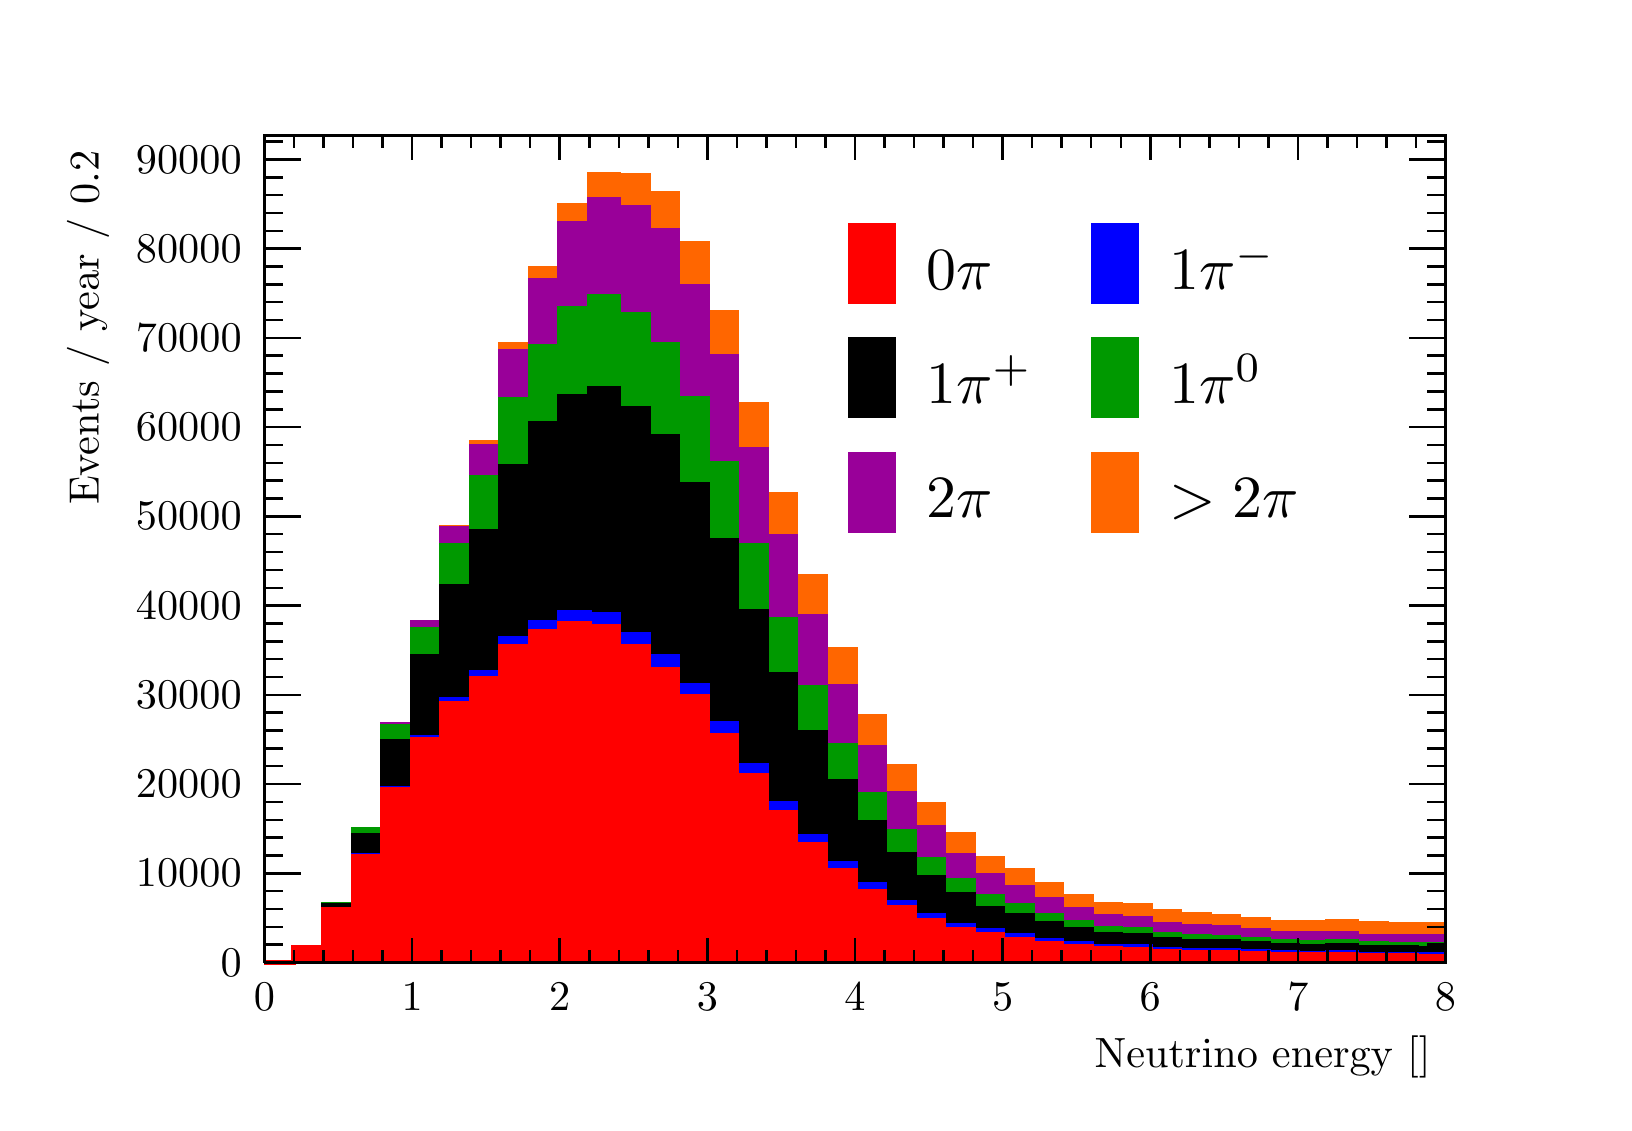
\begin{tikzpicture}
\pgfdeclareplotmark{cross} {
\pgfpathmoveto{\pgfpoint{-0.3\pgfplotmarksize}{\pgfplotmarksize}}
\pgfpathlineto{\pgfpoint{+0.3\pgfplotmarksize}{\pgfplotmarksize}}
\pgfpathlineto{\pgfpoint{+0.3\pgfplotmarksize}{0.3\pgfplotmarksize}}
\pgfpathlineto{\pgfpoint{+1\pgfplotmarksize}{0.3\pgfplotmarksize}}
\pgfpathlineto{\pgfpoint{+1\pgfplotmarksize}{-0.3\pgfplotmarksize}}
\pgfpathlineto{\pgfpoint{+0.3\pgfplotmarksize}{-0.3\pgfplotmarksize}}
\pgfpathlineto{\pgfpoint{+0.3\pgfplotmarksize}{-1.\pgfplotmarksize}}
\pgfpathlineto{\pgfpoint{-0.3\pgfplotmarksize}{-1.\pgfplotmarksize}}
\pgfpathlineto{\pgfpoint{-0.3\pgfplotmarksize}{-0.3\pgfplotmarksize}}
\pgfpathlineto{\pgfpoint{-1.\pgfplotmarksize}{-0.3\pgfplotmarksize}}
\pgfpathlineto{\pgfpoint{-1.\pgfplotmarksize}{0.3\pgfplotmarksize}}
\pgfpathlineto{\pgfpoint{-0.3\pgfplotmarksize}{0.3\pgfplotmarksize}}
\pgfpathclose
\pgfusepathqstroke
}
\pgfdeclareplotmark{cross*} {
\pgfpathmoveto{\pgfpoint{-0.3\pgfplotmarksize}{\pgfplotmarksize}}
\pgfpathlineto{\pgfpoint{+0.3\pgfplotmarksize}{\pgfplotmarksize}}
\pgfpathlineto{\pgfpoint{+0.3\pgfplotmarksize}{0.3\pgfplotmarksize}}
\pgfpathlineto{\pgfpoint{+1\pgfplotmarksize}{0.3\pgfplotmarksize}}
\pgfpathlineto{\pgfpoint{+1\pgfplotmarksize}{-0.3\pgfplotmarksize}}
\pgfpathlineto{\pgfpoint{+0.3\pgfplotmarksize}{-0.3\pgfplotmarksize}}
\pgfpathlineto{\pgfpoint{+0.3\pgfplotmarksize}{-1.\pgfplotmarksize}}
\pgfpathlineto{\pgfpoint{-0.3\pgfplotmarksize}{-1.\pgfplotmarksize}}
\pgfpathlineto{\pgfpoint{-0.3\pgfplotmarksize}{-0.3\pgfplotmarksize}}
\pgfpathlineto{\pgfpoint{-1.\pgfplotmarksize}{-0.3\pgfplotmarksize}}
\pgfpathlineto{\pgfpoint{-1.\pgfplotmarksize}{0.3\pgfplotmarksize}}
\pgfpathlineto{\pgfpoint{-0.3\pgfplotmarksize}{0.3\pgfplotmarksize}}
\pgfpathclose
\pgfusepathqfillstroke
}
\pgfdeclareplotmark{newstar} {
\pgfpathmoveto{\pgfqpoint{0pt}{\pgfplotmarksize}}
\pgfpathlineto{\pgfqpointpolar{44}{0.5\pgfplotmarksize}}
\pgfpathlineto{\pgfqpointpolar{18}{\pgfplotmarksize}}
\pgfpathlineto{\pgfqpointpolar{-20}{0.5\pgfplotmarksize}}
\pgfpathlineto{\pgfqpointpolar{-54}{\pgfplotmarksize}}
\pgfpathlineto{\pgfqpointpolar{-90}{0.5\pgfplotmarksize}}
\pgfpathlineto{\pgfqpointpolar{234}{\pgfplotmarksize}}
\pgfpathlineto{\pgfqpointpolar{198}{0.5\pgfplotmarksize}}
\pgfpathlineto{\pgfqpointpolar{162}{\pgfplotmarksize}}
\pgfpathlineto{\pgfqpointpolar{134}{0.5\pgfplotmarksize}}
\pgfpathclose
\pgfusepathqstroke
}
\pgfdeclareplotmark{newstar*} {
\pgfpathmoveto{\pgfqpoint{0pt}{\pgfplotmarksize}}
\pgfpathlineto{\pgfqpointpolar{44}{0.5\pgfplotmarksize}}
\pgfpathlineto{\pgfqpointpolar{18}{\pgfplotmarksize}}
\pgfpathlineto{\pgfqpointpolar{-20}{0.5\pgfplotmarksize}}
\pgfpathlineto{\pgfqpointpolar{-54}{\pgfplotmarksize}}
\pgfpathlineto{\pgfqpointpolar{-90}{0.5\pgfplotmarksize}}
\pgfpathlineto{\pgfqpointpolar{234}{\pgfplotmarksize}}
\pgfpathlineto{\pgfqpointpolar{198}{0.5\pgfplotmarksize}}
\pgfpathlineto{\pgfqpointpolar{162}{\pgfplotmarksize}}
\pgfpathlineto{\pgfqpointpolar{134}{0.5\pgfplotmarksize}}
\pgfpathclose
\pgfusepathqfillstroke
}
\definecolor{c}{rgb}{1,1,1};
\draw [color=c, fill=c] (0,0) rectangle (20,13.639);
\draw [color=c, fill=c] (3,1.77307) rectangle (18,12.2751);
\definecolor{c}{rgb}{0,0,0};
\draw [c,line width=0.9] (3,1.77307) -- (3,12.2751) -- (18,12.2751) -- (18,1.77307) -- (3,1.77307);
\definecolor{c}{rgb}{1,1,1};
\draw [color=c, fill=c] (3,1.77307) rectangle (18,12.2751);
\definecolor{c}{rgb}{0,0,0};
\draw [c,line width=0.9] (3,1.77307) -- (3,12.2751) -- (18,12.2751) -- (18,1.77307) -- (3,1.77307);
\draw [c,line width=0.9] (3,1.77307) -- (3.375,1.77307) -- (3.375,1.77307) -- (3.75,1.77307) -- (3.75,1.77307) -- (4.125,1.77307) -- (4.125,1.77307) -- (4.5,1.77307) -- (4.5,1.77307) -- (4.875,1.77307) -- (4.875,1.77307) -- (5.25,1.77307) --
 (5.25,1.77307) -- (5.625,1.77307) -- (5.625,1.77307) -- (6,1.77307) -- (6,1.77307) -- (6.375,1.77307) -- (6.375,1.77307) -- (6.75,1.77307) -- (6.75,1.77307) -- (7.125,1.77307) -- (7.125,1.77307) -- (7.5,1.77307) -- (7.5,1.77307) -- (7.875,1.77307)
 -- (7.875,1.77307) -- (8.25,1.77307) -- (8.25,1.77307) -- (8.625,1.77307) -- (8.625,1.77307) -- (9,1.77307) -- (9,1.77307) -- (9.375,1.77307) -- (9.375,1.77307) -- (9.75,1.77307) -- (9.75,1.77307) -- (10.125,1.77307) -- (10.125,1.77307) --
 (10.5,1.77307) -- (10.5,1.77307) -- (10.875,1.77307) -- (10.875,1.77307) -- (11.25,1.77307) -- (11.25,1.77307) -- (11.625,1.77307) -- (11.625,1.77307) -- (12,1.77307) -- (12,1.77307) -- (12.375,1.77307) -- (12.375,1.77307) -- (12.75,1.77307) --
 (12.75,1.77307) -- (13.125,1.77307) -- (13.125,1.77307) -- (13.5,1.77307) -- (13.5,1.77307) -- (13.875,1.77307) -- (13.875,1.77307) -- (14.25,1.77307) -- (14.25,1.77307) -- (14.625,1.77307) -- (14.625,1.77307) -- (15,1.77307) -- (15,1.77307) --
 (15.375,1.77307) -- (15.375,1.77307) -- (15.75,1.77307) -- (15.75,1.77307) -- (16.125,1.77307) -- (16.125,1.77307) -- (16.5,1.77307) -- (16.5,1.77307) -- (16.875,1.77307) -- (16.875,1.77307) -- (17.25,1.77307) -- (17.25,1.77307) -- (17.625,1.77307)
 -- (17.625,1.77307) -- (18,1.77307);
\draw [c,line width=0.9] (3,1.77307) -- (18,1.77307);
\draw [c,line width=0.9] (3,2.07994) -- (3,1.77307);
\draw [c,line width=0.9] (3.375,1.9265) -- (3.375,1.77307);
\draw [c,line width=0.9] (3.75,1.9265) -- (3.75,1.77307);
\draw [c,line width=0.9] (4.125,1.9265) -- (4.125,1.77307);
\draw [c,line width=0.9] (4.5,1.9265) -- (4.5,1.77307);
\draw [c,line width=0.9] (4.875,2.07994) -- (4.875,1.77307);
\draw [c,line width=0.9] (5.25,1.9265) -- (5.25,1.77307);
\draw [c,line width=0.9] (5.625,1.9265) -- (5.625,1.77307);
\draw [c,line width=0.9] (6,1.9265) -- (6,1.77307);
\draw [c,line width=0.9] (6.375,1.9265) -- (6.375,1.77307);
\draw [c,line width=0.9] (6.75,2.07994) -- (6.75,1.77307);
\draw [c,line width=0.9] (7.125,1.9265) -- (7.125,1.77307);
\draw [c,line width=0.9] (7.5,1.9265) -- (7.5,1.77307);
\draw [c,line width=0.9] (7.875,1.9265) -- (7.875,1.77307);
\draw [c,line width=0.9] (8.25,1.9265) -- (8.25,1.77307);
\draw [c,line width=0.9] (8.625,2.07994) -- (8.625,1.77307);
\draw [c,line width=0.9] (9,1.9265) -- (9,1.77307);
\draw [c,line width=0.9] (9.375,1.9265) -- (9.375,1.77307);
\draw [c,line width=0.9] (9.75,1.9265) -- (9.75,1.77307);
\draw [c,line width=0.9] (10.125,1.9265) -- (10.125,1.77307);
\draw [c,line width=0.9] (10.5,2.07994) -- (10.5,1.77307);
\draw [c,line width=0.9] (10.875,1.9265) -- (10.875,1.77307);
\draw [c,line width=0.9] (11.25,1.9265) -- (11.25,1.77307);
\draw [c,line width=0.9] (11.625,1.9265) -- (11.625,1.77307);
\draw [c,line width=0.9] (12,1.9265) -- (12,1.77307);
\draw [c,line width=0.9] (12.375,2.07994) -- (12.375,1.77307);
\draw [c,line width=0.9] (12.75,1.9265) -- (12.75,1.77307);
\draw [c,line width=0.9] (13.125,1.9265) -- (13.125,1.77307);
\draw [c,line width=0.9] (13.5,1.9265) -- (13.5,1.77307);
\draw [c,line width=0.9] (13.875,1.9265) -- (13.875,1.77307);
\draw [c,line width=0.9] (14.25,2.07994) -- (14.25,1.77307);
\draw [c,line width=0.9] (14.625,1.9265) -- (14.625,1.77307);
\draw [c,line width=0.9] (15,1.9265) -- (15,1.77307);
\draw [c,line width=0.9] (15.375,1.9265) -- (15.375,1.77307);
\draw [c,line width=0.9] (15.75,1.9265) -- (15.75,1.77307);
\draw [c,line width=0.9] (16.125,2.07994) -- (16.125,1.77307);
\draw [c,line width=0.9] (16.5,1.9265) -- (16.5,1.77307);
\draw [c,line width=0.9] (16.875,1.9265) -- (16.875,1.77307);
\draw [c,line width=0.9] (17.25,1.9265) -- (17.25,1.77307);
\draw [c,line width=0.9] (17.625,1.9265) -- (17.625,1.77307);
\draw [c,line width=0.9] (18,2.07994) -- (18,1.77307);
\draw [anchor=base] (3,1.15931) node[scale=1.52731, color=c, rotate=0]{0};
\draw [anchor=base] (4.875,1.15931) node[scale=1.52731, color=c, rotate=0]{1};
\draw [anchor=base] (6.75,1.15931) node[scale=1.52731, color=c, rotate=0]{2};
\draw [anchor=base] (8.625,1.15931) node[scale=1.52731, color=c, rotate=0]{3};
\draw [anchor=base] (10.5,1.15931) node[scale=1.52731, color=c, rotate=0]{4};
\draw [anchor=base] (12.375,1.15931) node[scale=1.52731, color=c, rotate=0]{5};
\draw [anchor=base] (14.25,1.15931) node[scale=1.52731, color=c, rotate=0]{6};
\draw [anchor=base] (16.125,1.15931) node[scale=1.52731, color=c, rotate=0]{7};
\draw [anchor=base] (18,1.15931) node[scale=1.52731, color=c, rotate=0]{8};
\draw [anchor= east] (18,0.572837) node[scale=1.52731, color=c, rotate=0]{ Neutrino energy [\si{\giga\electronvolt}]};
\draw [c,line width=0.9] (3,12.2751) -- (18,12.2751);
\draw [c,line width=0.9] (3,11.9682) -- (3,12.2751);
\draw [c,line width=0.9] (3.375,12.1216) -- (3.375,12.2751);
\draw [c,line width=0.9] (3.75,12.1216) -- (3.75,12.2751);
\draw [c,line width=0.9] (4.125,12.1216) -- (4.125,12.2751);
\draw [c,line width=0.9] (4.5,12.1216) -- (4.5,12.2751);
\draw [c,line width=0.9] (4.875,11.9682) -- (4.875,12.2751);
\draw [c,line width=0.9] (5.25,12.1216) -- (5.25,12.2751);
\draw [c,line width=0.9] (5.625,12.1216) -- (5.625,12.2751);
\draw [c,line width=0.9] (6,12.1216) -- (6,12.2751);
\draw [c,line width=0.9] (6.375,12.1216) -- (6.375,12.2751);
\draw [c,line width=0.9] (6.75,11.9682) -- (6.75,12.2751);
\draw [c,line width=0.9] (7.125,12.1216) -- (7.125,12.2751);
\draw [c,line width=0.9] (7.5,12.1216) -- (7.5,12.2751);
\draw [c,line width=0.9] (7.875,12.1216) -- (7.875,12.2751);
\draw [c,line width=0.9] (8.25,12.1216) -- (8.25,12.2751);
\draw [c,line width=0.9] (8.625,11.9682) -- (8.625,12.2751);
\draw [c,line width=0.9] (9,12.1216) -- (9,12.2751);
\draw [c,line width=0.9] (9.375,12.1216) -- (9.375,12.2751);
\draw [c,line width=0.9] (9.75,12.1216) -- (9.75,12.2751);
\draw [c,line width=0.9] (10.125,12.1216) -- (10.125,12.2751);
\draw [c,line width=0.9] (10.5,11.9682) -- (10.5,12.2751);
\draw [c,line width=0.9] (10.875,12.1216) -- (10.875,12.2751);
\draw [c,line width=0.9] (11.25,12.1216) -- (11.25,12.2751);
\draw [c,line width=0.9] (11.625,12.1216) -- (11.625,12.2751);
\draw [c,line width=0.9] (12,12.1216) -- (12,12.2751);
\draw [c,line width=0.9] (12.375,11.9682) -- (12.375,12.2751);
\draw [c,line width=0.9] (12.75,12.1216) -- (12.75,12.2751);
\draw [c,line width=0.9] (13.125,12.1216) -- (13.125,12.2751);
\draw [c,line width=0.9] (13.5,12.1216) -- (13.5,12.2751);
\draw [c,line width=0.9] (13.875,12.1216) -- (13.875,12.2751);
\draw [c,line width=0.9] (14.25,11.9682) -- (14.25,12.2751);
\draw [c,line width=0.9] (14.625,12.1216) -- (14.625,12.2751);
\draw [c,line width=0.9] (15,12.1216) -- (15,12.2751);
\draw [c,line width=0.9] (15.375,12.1216) -- (15.375,12.2751);
\draw [c,line width=0.9] (15.75,12.1216) -- (15.75,12.2751);
\draw [c,line width=0.9] (16.125,11.9682) -- (16.125,12.2751);
\draw [c,line width=0.9] (16.5,12.1216) -- (16.5,12.2751);
\draw [c,line width=0.9] (16.875,12.1216) -- (16.875,12.2751);
\draw [c,line width=0.9] (17.25,12.1216) -- (17.25,12.2751);
\draw [c,line width=0.9] (17.625,12.1216) -- (17.625,12.2751);
\draw [c,line width=0.9] (18,11.9682) -- (18,12.2751);
\draw [c,line width=0.9] (3,1.77307) -- (3,12.2751);
\draw [c,line width=0.9] (3.462,1.77307) -- (3,1.77307);
\draw [c,line width=0.9] (3.231,1.99972) -- (3,1.99972);
\draw [c,line width=0.9] (3.231,2.22638) -- (3,2.22638);
\draw [c,line width=0.9] (3.231,2.45304) -- (3,2.45304);
\draw [c,line width=0.9] (3.231,2.67969) -- (3,2.67969);
\draw [c,line width=0.9] (3.462,2.90635) -- (3,2.90635);
\draw [c,line width=0.9] (3.231,3.13301) -- (3,3.13301);
\draw [c,line width=0.9] (3.231,3.35967) -- (3,3.35967);
\draw [c,line width=0.9] (3.231,3.58632) -- (3,3.58632);
\draw [c,line width=0.9] (3.231,3.81298) -- (3,3.81298);
\draw [c,line width=0.9] (3.462,4.03964) -- (3,4.03964);
\draw [c,line width=0.9] (3.231,4.26629) -- (3,4.26629);
\draw [c,line width=0.9] (3.231,4.49295) -- (3,4.49295);
\draw [c,line width=0.9] (3.231,4.71961) -- (3,4.71961);
\draw [c,line width=0.9] (3.231,4.94626) -- (3,4.94626);
\draw [c,line width=0.9] (3.462,5.17292) -- (3,5.17292);
\draw [c,line width=0.9] (3.231,5.39958) -- (3,5.39958);
\draw [c,line width=0.9] (3.231,5.62624) -- (3,5.62624);
\draw [c,line width=0.9] (3.231,5.85289) -- (3,5.85289);
\draw [c,line width=0.9] (3.231,6.07955) -- (3,6.07955);
\draw [c,line width=0.9] (3.462,6.30621) -- (3,6.30621);
\draw [c,line width=0.9] (3.231,6.53286) -- (3,6.53286);
\draw [c,line width=0.9] (3.231,6.75952) -- (3,6.75952);
\draw [c,line width=0.9] (3.231,6.98618) -- (3,6.98618);
\draw [c,line width=0.9] (3.231,7.21283) -- (3,7.21283);
\draw [c,line width=0.9] (3.462,7.43949) -- (3,7.43949);
\draw [c,line width=0.9] (3.231,7.66615) -- (3,7.66615);
\draw [c,line width=0.9] (3.231,7.89281) -- (3,7.89281);
\draw [c,line width=0.9] (3.231,8.11946) -- (3,8.11946);
\draw [c,line width=0.9] (3.231,8.34612) -- (3,8.34612);
\draw [c,line width=0.9] (3.462,8.57278) -- (3,8.57278);
\draw [c,line width=0.9] (3.231,8.79943) -- (3,8.79943);
\draw [c,line width=0.9] (3.231,9.02609) -- (3,9.02609);
\draw [c,line width=0.9] (3.231,9.25275) -- (3,9.25275);
\draw [c,line width=0.9] (3.231,9.4794) -- (3,9.4794);
\draw [c,line width=0.9] (3.462,9.70606) -- (3,9.70606);
\draw [c,line width=0.9] (3.231,9.93272) -- (3,9.93272);
\draw [c,line width=0.9] (3.231,10.1594) -- (3,10.1594);
\draw [c,line width=0.9] (3.231,10.386) -- (3,10.386);
\draw [c,line width=0.9] (3.231,10.6127) -- (3,10.6127);
\draw [c,line width=0.9] (3.462,10.8393) -- (3,10.8393);
\draw [c,line width=0.9] (3.231,11.066) -- (3,11.066);
\draw [c,line width=0.9] (3.231,11.2927) -- (3,11.2927);
\draw [c,line width=0.9] (3.231,11.5193) -- (3,11.5193);
\draw [c,line width=0.9] (3.231,11.746) -- (3,11.746);
\draw [c,line width=0.9] (3.462,11.9726) -- (3,11.9726);
\draw [c,line width=0.9] (3.462,11.9726) -- (3,11.9726);
\draw [c,line width=0.9] (3.231,12.1993) -- (3,12.1993);
\draw [anchor= east] (2.9,1.77307) node[scale=1.52731, color=c, rotate=0]{0};
\draw [anchor= east] (2.9,2.90635) node[scale=1.52731, color=c, rotate=0]{10000};
\draw [anchor= east] (2.9,4.03964) node[scale=1.52731, color=c, rotate=0]{20000};
\draw [anchor= east] (2.9,5.17292) node[scale=1.52731, color=c, rotate=0]{30000};
\draw [anchor= east] (2.9,6.30621) node[scale=1.52731, color=c, rotate=0]{40000};
\draw [anchor= east] (2.9,7.43949) node[scale=1.52731, color=c, rotate=0]{50000};
\draw [anchor= east] (2.9,8.57278) node[scale=1.52731, color=c, rotate=0]{60000};
\draw [anchor= east] (2.9,9.70606) node[scale=1.52731, color=c, rotate=0]{70000};
\draw [anchor= east] (2.9,10.8393) node[scale=1.52731, color=c, rotate=0]{80000};
\draw [anchor= east] (2.9,11.9726) node[scale=1.52731, color=c, rotate=0]{90000};
\draw [anchor= east] (0.76,12.2751) node[scale=1.52731, color=c, rotate=90]{ Events / year / \SI{0.2}{\giga\electronvolt} };
\draw [c,line width=0.9] (18,1.77307) -- (18,12.2751);
\draw [c,line width=0.9] (17.538,1.77307) -- (18,1.77307);
\draw [c,line width=0.9] (17.769,1.99972) -- (18,1.99972);
\draw [c,line width=0.9] (17.769,2.22638) -- (18,2.22638);
\draw [c,line width=0.9] (17.769,2.45304) -- (18,2.45304);
\draw [c,line width=0.9] (17.769,2.67969) -- (18,2.67969);
\draw [c,line width=0.9] (17.538,2.90635) -- (18,2.90635);
\draw [c,line width=0.9] (17.769,3.13301) -- (18,3.13301);
\draw [c,line width=0.9] (17.769,3.35967) -- (18,3.35967);
\draw [c,line width=0.9] (17.769,3.58632) -- (18,3.58632);
\draw [c,line width=0.9] (17.769,3.81298) -- (18,3.81298);
\draw [c,line width=0.9] (17.538,4.03964) -- (18,4.03964);
\draw [c,line width=0.9] (17.769,4.26629) -- (18,4.26629);
\draw [c,line width=0.9] (17.769,4.49295) -- (18,4.49295);
\draw [c,line width=0.9] (17.769,4.71961) -- (18,4.71961);
\draw [c,line width=0.9] (17.769,4.94626) -- (18,4.94626);
\draw [c,line width=0.9] (17.538,5.17292) -- (18,5.17292);
\draw [c,line width=0.9] (17.769,5.39958) -- (18,5.39958);
\draw [c,line width=0.9] (17.769,5.62624) -- (18,5.62624);
\draw [c,line width=0.9] (17.769,5.85289) -- (18,5.85289);
\draw [c,line width=0.9] (17.769,6.07955) -- (18,6.07955);
\draw [c,line width=0.9] (17.538,6.30621) -- (18,6.30621);
\draw [c,line width=0.9] (17.769,6.53286) -- (18,6.53286);
\draw [c,line width=0.9] (17.769,6.75952) -- (18,6.75952);
\draw [c,line width=0.9] (17.769,6.98618) -- (18,6.98618);
\draw [c,line width=0.9] (17.769,7.21283) -- (18,7.21283);
\draw [c,line width=0.9] (17.538,7.43949) -- (18,7.43949);
\draw [c,line width=0.9] (17.769,7.66615) -- (18,7.66615);
\draw [c,line width=0.9] (17.769,7.89281) -- (18,7.89281);
\draw [c,line width=0.9] (17.769,8.11946) -- (18,8.11946);
\draw [c,line width=0.9] (17.769,8.34612) -- (18,8.34612);
\draw [c,line width=0.9] (17.538,8.57278) -- (18,8.57278);
\draw [c,line width=0.9] (17.769,8.79943) -- (18,8.79943);
\draw [c,line width=0.9] (17.769,9.02609) -- (18,9.02609);
\draw [c,line width=0.9] (17.769,9.25275) -- (18,9.25275);
\draw [c,line width=0.9] (17.769,9.4794) -- (18,9.4794);
\draw [c,line width=0.9] (17.538,9.70606) -- (18,9.70606);
\draw [c,line width=0.9] (17.769,9.93272) -- (18,9.93272);
\draw [c,line width=0.9] (17.769,10.1594) -- (18,10.1594);
\draw [c,line width=0.9] (17.769,10.386) -- (18,10.386);
\draw [c,line width=0.9] (17.769,10.6127) -- (18,10.6127);
\draw [c,line width=0.9] (17.538,10.8393) -- (18,10.8393);
\draw [c,line width=0.9] (17.769,11.066) -- (18,11.066);
\draw [c,line width=0.9] (17.769,11.2927) -- (18,11.2927);
\draw [c,line width=0.9] (17.769,11.5193) -- (18,11.5193);
\draw [c,line width=0.9] (17.769,11.746) -- (18,11.746);
\draw [c,line width=0.9] (17.538,11.9726) -- (18,11.9726);
\draw [c,line width=0.9] (17.538,11.9726) -- (18,11.9726);
\draw [c,line width=0.9] (17.769,12.1993) -- (18,12.1993);
\definecolor{c}{rgb}{1,0.4,0};
\draw [c, fill=c] (3,1.77307) -- (3,1.779) -- (3.375,1.779) -- (3.375,1.95842) -- (3.75,1.95842) -- (3.75,2.50479) -- (4.125,2.50479) -- (4.125,3.46262) -- (4.5,3.46262) -- (4.5,4.79128) -- (4.875,4.79128) -- (4.875,6.09505) -- (5.25,6.09505) --
 (5.25,7.29305) -- (5.625,7.29305) -- (5.625,8.37548) -- (6,8.37548) -- (6,9.61824) -- (6.375,9.61824) -- (6.375,10.5866) -- (6.75,10.5866) -- (6.75,11.3838) -- (7.125,11.3838) -- (7.125,11.775) -- (7.5,11.775) -- (7.5,11.7652) -- (7.875,11.7652) --
 (7.875,11.5346) -- (8.25,11.5346) -- (8.25,10.8989) -- (8.625,10.8989) -- (8.625,10.0316) -- (9,10.0316) -- (9,8.85685) -- (9.375,8.85685) -- (9.375,7.71973) -- (9.75,7.71973) -- (9.75,6.67058) -- (10.125,6.67058) -- (10.125,5.74628) --
 (10.5,5.74628) -- (10.5,4.90157) -- (10.875,4.90157) -- (10.875,4.25819) -- (11.25,4.25819) -- (11.25,3.77863) -- (11.625,3.77863) -- (11.625,3.39323) -- (12,3.39323) -- (12,3.10044) -- (12.375,3.10044) -- (12.375,2.94088) -- (12.75,2.94088) --
 (12.75,2.76379) -- (13.125,2.76379) -- (13.125,2.61198) -- (13.5,2.61198) -- (13.5,2.51279) -- (13.875,2.51279) -- (13.875,2.49138) -- (14.25,2.49138) -- (14.25,2.41618) -- (14.625,2.41618) -- (14.625,2.38277) -- (15,2.38277) -- (15,2.35543) --
 (15.375,2.35543) -- (15.375,2.32473) -- (15.75,2.32473) -- (15.75,2.27584) -- (16.125,2.27584) -- (16.125,2.28255) -- (16.5,2.28255) -- (16.5,2.29042) -- (16.875,2.29042) -- (16.875,2.2654) -- (17.25,2.2654) -- (17.25,2.25147) -- (17.625,2.25147) --
 (17.625,2.25959) -- (18,2.25959) -- (18,1.77307);
\draw [c,line width=1.8] (3,1.779) -- (3.375,1.779) -- (3.375,1.95842) -- (3.75,1.95842) -- (3.75,2.50479) -- (4.125,2.50479) -- (4.125,3.46262) -- (4.5,3.46262) -- (4.5,4.79128) -- (4.875,4.79128) -- (4.875,6.09505) -- (5.25,6.09505) --
 (5.25,7.29305) -- (5.625,7.29305) -- (5.625,8.37548) -- (6,8.37548) -- (6,9.61824) -- (6.375,9.61824) -- (6.375,10.5866) -- (6.75,10.5866) -- (6.75,11.3838) -- (7.125,11.3838) -- (7.125,11.775) -- (7.5,11.775) -- (7.5,11.7652) -- (7.875,11.7652) --
 (7.875,11.5346) -- (8.25,11.5346) -- (8.25,10.8989) -- (8.625,10.8989) -- (8.625,10.0316) -- (9,10.0316) -- (9,8.85685) -- (9.375,8.85685) -- (9.375,7.71973) -- (9.75,7.71973) -- (9.75,6.67058) -- (10.125,6.67058) -- (10.125,5.74628) --
 (10.5,5.74628) -- (10.5,4.90157) -- (10.875,4.90157) -- (10.875,4.25819) -- (11.25,4.25819) -- (11.25,3.77863) -- (11.625,3.77863) -- (11.625,3.39323) -- (12,3.39323) -- (12,3.10044) -- (12.375,3.10044) -- (12.375,2.94088) -- (12.75,2.94088) --
 (12.75,2.76379) -- (13.125,2.76379) -- (13.125,2.61198) -- (13.5,2.61198) -- (13.5,2.51279) -- (13.875,2.51279) -- (13.875,2.49138) -- (14.25,2.49138) -- (14.25,2.41618) -- (14.625,2.41618) -- (14.625,2.38277) -- (15,2.38277) -- (15,2.35543) --
 (15.375,2.35543) -- (15.375,2.32473) -- (15.75,2.32473) -- (15.75,2.27584) -- (16.125,2.27584) -- (16.125,2.28255) -- (16.5,2.28255) -- (16.5,2.29042) -- (16.875,2.29042) -- (16.875,2.2654) -- (17.25,2.2654) -- (17.25,2.25147) -- (17.625,2.25147) --
 (17.625,2.25959) -- (18,2.25959);
\definecolor{c}{rgb}{0.999,0.999,0.999};
\draw [c, fill=c] (3,1.77307) -- (3,1.779) -- (3.375,1.779) -- (3.375,1.95842) -- (3.75,1.95842) -- (3.75,2.50479) -- (4.125,2.50479) -- (4.125,3.46262) -- (4.5,3.46262) -- (4.5,4.79038) -- (4.875,4.79038) -- (4.875,6.09054) -- (5.25,6.09054) --
 (5.25,7.27977) -- (5.625,7.27977) -- (5.625,8.33189) -- (6,8.33189) -- (6,9.53569) -- (6.375,9.53569) -- (6.375,10.4404) -- (6.75,10.4404) -- (6.75,11.16) -- (7.125,11.16) -- (7.125,11.4684) -- (7.5,11.4684) -- (7.5,11.3638) -- (7.875,11.3638) --
 (7.875,11.0662) -- (8.25,11.0662) -- (8.25,10.3595) -- (8.625,10.3595) -- (8.625,9.46784) -- (9,9.46784) -- (9,8.28687) -- (9.375,8.28687) -- (9.375,7.18148) -- (9.75,7.18148) -- (9.75,6.17193) -- (10.125,6.17193) -- (10.125,5.28207) --
 (10.5,5.28207) -- (10.5,4.51023) -- (10.875,4.51023) -- (10.875,3.92632) -- (11.25,3.92632) -- (11.25,3.48997) -- (11.625,3.48997) -- (11.625,3.13707) -- (12,3.13707) -- (12,2.87768) -- (12.375,2.87768) -- (12.375,2.7318) -- (12.75,2.7318) --
 (12.75,2.56993) -- (13.125,2.56993) -- (13.125,2.44688) -- (13.5,2.44688) -- (13.5,2.35517) -- (13.875,2.35517) -- (13.875,2.3384) -- (14.25,2.3384) -- (14.25,2.26191) -- (14.625,2.26191) -- (14.625,2.23199) -- (15,2.23199) -- (15,2.21393) --
 (15.375,2.21393) -- (15.375,2.17911) -- (15.75,2.17911) -- (15.75,2.14144) -- (16.125,2.14144) -- (16.125,2.13835) -- (16.5,2.13835) -- (16.5,2.1448) -- (16.875,2.1448) -- (16.875,2.10804) -- (17.25,2.10804) -- (17.25,2.10417) -- (17.625,2.10417) --
 (17.625,2.10726) -- (18,2.10726) -- (18,1.77307);
\definecolor{c}{rgb}{0.6,0,0.6};
\draw [c,line width=1.8] (3,1.779) -- (3.375,1.779) -- (3.375,1.95842) -- (3.75,1.95842) -- (3.75,2.50479) -- (4.125,2.50479) -- (4.125,3.46262) -- (4.5,3.46262) -- (4.5,4.79038) -- (4.875,4.79038) -- (4.875,6.09054) -- (5.25,6.09054) --
 (5.25,7.27977) -- (5.625,7.27977) -- (5.625,8.33189) -- (6,8.33189) -- (6,9.53569) -- (6.375,9.53569) -- (6.375,10.4404) -- (6.75,10.4404) -- (6.75,11.16) -- (7.125,11.16) -- (7.125,11.4684) -- (7.5,11.4684) -- (7.5,11.3638) -- (7.875,11.3638) --
 (7.875,11.0662) -- (8.25,11.0662) -- (8.25,10.3595) -- (8.625,10.3595) -- (8.625,9.46784) -- (9,9.46784) -- (9,8.28687) -- (9.375,8.28687) -- (9.375,7.18148) -- (9.75,7.18148) -- (9.75,6.17193) -- (10.125,6.17193) -- (10.125,5.28207) --
 (10.5,5.28207) -- (10.5,4.51023) -- (10.875,4.51023) -- (10.875,3.92632) -- (11.25,3.92632) -- (11.25,3.48997) -- (11.625,3.48997) -- (11.625,3.13707) -- (12,3.13707) -- (12,2.87768) -- (12.375,2.87768) -- (12.375,2.7318) -- (12.75,2.7318) --
 (12.75,2.56993) -- (13.125,2.56993) -- (13.125,2.44688) -- (13.5,2.44688) -- (13.5,2.35517) -- (13.875,2.35517) -- (13.875,2.3384) -- (14.25,2.3384) -- (14.25,2.26191) -- (14.625,2.26191) -- (14.625,2.23199) -- (15,2.23199) -- (15,2.21393) --
 (15.375,2.21393) -- (15.375,2.17911) -- (15.75,2.17911) -- (15.75,2.14144) -- (16.125,2.14144) -- (16.125,2.13835) -- (16.5,2.13835) -- (16.5,2.1448) -- (16.875,2.1448) -- (16.875,2.10804) -- (17.25,2.10804) -- (17.25,2.10417) -- (17.625,2.10417) --
 (17.625,2.10726) -- (18,2.10726);
\draw [c,line width=1.8] (3,1.779) -- (3.375,1.779) -- (3.375,1.95842) -- (3.75,1.95842) -- (3.75,2.50479) -- (4.125,2.50479) -- (4.125,3.46262) -- (4.5,3.46262) -- (4.5,4.79038) -- (4.875,4.79038) -- (4.875,6.09054) -- (5.25,6.09054) --
 (5.25,7.27977) -- (5.625,7.27977) -- (5.625,8.33189) -- (6,8.33189) -- (6,9.53569) -- (6.375,9.53569) -- (6.375,10.4404) -- (6.75,10.4404) -- (6.75,11.16) -- (7.125,11.16) -- (7.125,11.4684) -- (7.5,11.4684) -- (7.5,11.3638) -- (7.875,11.3638) --
 (7.875,11.0662) -- (8.25,11.0662) -- (8.25,10.3595) -- (8.625,10.3595) -- (8.625,9.46784) -- (9,9.46784) -- (9,8.28687) -- (9.375,8.28687) -- (9.375,7.18148) -- (9.75,7.18148) -- (9.75,6.17193) -- (10.125,6.17193) -- (10.125,5.28207) --
 (10.5,5.28207) -- (10.5,4.51023) -- (10.875,4.51023) -- (10.875,3.92632) -- (11.25,3.92632) -- (11.25,3.48997) -- (11.625,3.48997) -- (11.625,3.13707) -- (12,3.13707) -- (12,2.87768) -- (12.375,2.87768) -- (12.375,2.7318) -- (12.75,2.7318) --
 (12.75,2.56993) -- (13.125,2.56993) -- (13.125,2.44688) -- (13.5,2.44688) -- (13.5,2.35517) -- (13.875,2.35517) -- (13.875,2.3384) -- (14.25,2.3384) -- (14.25,2.26191) -- (14.625,2.26191) -- (14.625,2.23199) -- (15,2.23199) -- (15,2.21393) --
 (15.375,2.21393) -- (15.375,2.17911) -- (15.75,2.17911) -- (15.75,2.14144) -- (16.125,2.14144) -- (16.125,2.13835) -- (16.5,2.13835) -- (16.5,2.1448) -- (16.875,2.1448) -- (16.875,2.10804) -- (17.25,2.10804) -- (17.25,2.10417) -- (17.625,2.10417) --
 (17.625,2.10726) -- (18,2.10726);
\draw [c, fill=c] (3,1.77307) -- (3,1.779) -- (3.375,1.779) -- (3.375,1.95842) -- (3.75,1.95842) -- (3.75,2.50479) -- (4.125,2.50479) -- (4.125,3.46262) -- (4.5,3.46262) -- (4.5,4.79038) -- (4.875,4.79038) -- (4.875,6.09054) -- (5.25,6.09054) --
 (5.25,7.27977) -- (5.625,7.27977) -- (5.625,8.33189) -- (6,8.33189) -- (6,9.53569) -- (6.375,9.53569) -- (6.375,10.4404) -- (6.75,10.4404) -- (6.75,11.16) -- (7.125,11.16) -- (7.125,11.4684) -- (7.5,11.4684) -- (7.5,11.3638) -- (7.875,11.3638) --
 (7.875,11.0662) -- (8.25,11.0662) -- (8.25,10.3595) -- (8.625,10.3595) -- (8.625,9.46784) -- (9,9.46784) -- (9,8.28687) -- (9.375,8.28687) -- (9.375,7.18148) -- (9.75,7.18148) -- (9.75,6.17193) -- (10.125,6.17193) -- (10.125,5.28207) --
 (10.5,5.28207) -- (10.5,4.51023) -- (10.875,4.51023) -- (10.875,3.92632) -- (11.25,3.92632) -- (11.25,3.48997) -- (11.625,3.48997) -- (11.625,3.13707) -- (12,3.13707) -- (12,2.87768) -- (12.375,2.87768) -- (12.375,2.7318) -- (12.75,2.7318) --
 (12.75,2.56993) -- (13.125,2.56993) -- (13.125,2.44688) -- (13.5,2.44688) -- (13.5,2.35517) -- (13.875,2.35517) -- (13.875,2.3384) -- (14.25,2.3384) -- (14.25,2.26191) -- (14.625,2.26191) -- (14.625,2.23199) -- (15,2.23199) -- (15,2.21393) --
 (15.375,2.21393) -- (15.375,2.17911) -- (15.75,2.17911) -- (15.75,2.14144) -- (16.125,2.14144) -- (16.125,2.13835) -- (16.5,2.13835) -- (16.5,2.1448) -- (16.875,2.1448) -- (16.875,2.10804) -- (17.25,2.10804) -- (17.25,2.10417) -- (17.625,2.10417) --
 (17.625,2.10726) -- (18,2.10726) -- (18,1.77307);
\draw [c,line width=1.8] (3,1.779) -- (3.375,1.779) -- (3.375,1.95842) -- (3.75,1.95842) -- (3.75,2.50479) -- (4.125,2.50479) -- (4.125,3.46262) -- (4.5,3.46262) -- (4.5,4.79038) -- (4.875,4.79038) -- (4.875,6.09054) -- (5.25,6.09054) --
 (5.25,7.27977) -- (5.625,7.27977) -- (5.625,8.33189) -- (6,8.33189) -- (6,9.53569) -- (6.375,9.53569) -- (6.375,10.4404) -- (6.75,10.4404) -- (6.75,11.16) -- (7.125,11.16) -- (7.125,11.4684) -- (7.5,11.4684) -- (7.5,11.3638) -- (7.875,11.3638) --
 (7.875,11.0662) -- (8.25,11.0662) -- (8.25,10.3595) -- (8.625,10.3595) -- (8.625,9.46784) -- (9,9.46784) -- (9,8.28687) -- (9.375,8.28687) -- (9.375,7.18148) -- (9.75,7.18148) -- (9.75,6.17193) -- (10.125,6.17193) -- (10.125,5.28207) --
 (10.5,5.28207) -- (10.5,4.51023) -- (10.875,4.51023) -- (10.875,3.92632) -- (11.25,3.92632) -- (11.25,3.48997) -- (11.625,3.48997) -- (11.625,3.13707) -- (12,3.13707) -- (12,2.87768) -- (12.375,2.87768) -- (12.375,2.7318) -- (12.75,2.7318) --
 (12.75,2.56993) -- (13.125,2.56993) -- (13.125,2.44688) -- (13.5,2.44688) -- (13.5,2.35517) -- (13.875,2.35517) -- (13.875,2.3384) -- (14.25,2.3384) -- (14.25,2.26191) -- (14.625,2.26191) -- (14.625,2.23199) -- (15,2.23199) -- (15,2.21393) --
 (15.375,2.21393) -- (15.375,2.17911) -- (15.75,2.17911) -- (15.75,2.14144) -- (16.125,2.14144) -- (16.125,2.13835) -- (16.5,2.13835) -- (16.5,2.1448) -- (16.875,2.1448) -- (16.875,2.10804) -- (17.25,2.10804) -- (17.25,2.10417) -- (17.625,2.10417) --
 (17.625,2.10726) -- (18,2.10726);
\definecolor{c}{rgb}{0.999,0.999,0.999};
\draw [c, fill=c] (3,1.77307) -- (3,1.779) -- (3.375,1.779) -- (3.375,1.95842) -- (3.75,1.95842) -- (3.75,2.50479) -- (4.125,2.50479) -- (4.125,3.46133) -- (4.5,3.46133) -- (4.5,4.77581) -- (4.875,4.77581) -- (4.875,6.00812) -- (5.25,6.00812) --
 (5.25,7.06501) -- (5.625,7.06501) -- (5.625,7.93603) -- (6,7.93603) -- (6,8.91954) -- (6.375,8.91954) -- (6.375,9.59373) -- (6.75,9.59373) -- (6.75,10.0792) -- (7.125,10.0792) -- (7.125,10.2305) -- (7.5,10.2305) -- (7.5,10.0021) -- (7.875,10.0021)
 -- (7.875,9.61682) -- (8.25,9.61682) -- (8.25,8.93114) -- (8.625,8.93114) -- (8.625,8.11119) -- (9,8.11119) -- (9,7.07004) -- (9.375,7.07004) -- (9.375,6.12975) -- (9.75,6.12975) -- (9.75,5.26478) -- (10.125,5.26478) -- (10.125,4.53035) --
 (10.5,4.53035) -- (10.5,3.90401) -- (10.875,3.90401) -- (10.875,3.43579) -- (11.25,3.43579) -- (11.25,3.07774) -- (11.625,3.07774) -- (11.625,2.80984) -- (12,2.80984) -- (12,2.60759) -- (12.375,2.60759) -- (12.375,2.49654) -- (12.75,2.49654) --
 (12.75,2.37078) -- (13.125,2.37078) -- (13.125,2.27559) -- (13.5,2.27559) -- (13.5,2.20658) -- (13.875,2.20658) -- (13.875,2.18878) -- (14.25,2.18878) -- (14.25,2.1279) -- (14.625,2.1279) -- (14.625,2.09862) -- (15,2.09862) -- (15,2.09037) --
 (15.375,2.09037) -- (15.375,2.06779) -- (15.75,2.06779) -- (15.75,2.04019) -- (16.125,2.04019) -- (16.125,2.03078) -- (16.5,2.03078) -- (16.5,2.04122) -- (16.875,2.04122) -- (16.875,2.01143) -- (17.25,2.01143) -- (17.25,2.00343) -- (17.625,2.00343)
 -- (17.625,2.00008) -- (18,2.00008) -- (18,1.77307);
\definecolor{c}{rgb}{0,0.6,0};
\draw [c,line width=1.8] (3,1.779) -- (3.375,1.779) -- (3.375,1.95842) -- (3.75,1.95842) -- (3.75,2.50479) -- (4.125,2.50479) -- (4.125,3.46133) -- (4.5,3.46133) -- (4.5,4.77581) -- (4.875,4.77581) -- (4.875,6.00812) -- (5.25,6.00812) --
 (5.25,7.06501) -- (5.625,7.06501) -- (5.625,7.93603) -- (6,7.93603) -- (6,8.91954) -- (6.375,8.91954) -- (6.375,9.59373) -- (6.75,9.59373) -- (6.75,10.0792) -- (7.125,10.0792) -- (7.125,10.2305) -- (7.5,10.2305) -- (7.5,10.0021) -- (7.875,10.0021)
 -- (7.875,9.61682) -- (8.25,9.61682) -- (8.25,8.93114) -- (8.625,8.93114) -- (8.625,8.11119) -- (9,8.11119) -- (9,7.07004) -- (9.375,7.07004) -- (9.375,6.12975) -- (9.75,6.12975) -- (9.75,5.26478) -- (10.125,5.26478) -- (10.125,4.53035) --
 (10.5,4.53035) -- (10.5,3.90401) -- (10.875,3.90401) -- (10.875,3.43579) -- (11.25,3.43579) -- (11.25,3.07774) -- (11.625,3.07774) -- (11.625,2.80984) -- (12,2.80984) -- (12,2.60759) -- (12.375,2.60759) -- (12.375,2.49654) -- (12.75,2.49654) --
 (12.75,2.37078) -- (13.125,2.37078) -- (13.125,2.27559) -- (13.5,2.27559) -- (13.5,2.20658) -- (13.875,2.20658) -- (13.875,2.18878) -- (14.25,2.18878) -- (14.25,2.1279) -- (14.625,2.1279) -- (14.625,2.09862) -- (15,2.09862) -- (15,2.09037) --
 (15.375,2.09037) -- (15.375,2.06779) -- (15.75,2.06779) -- (15.75,2.04019) -- (16.125,2.04019) -- (16.125,2.03078) -- (16.5,2.03078) -- (16.5,2.04122) -- (16.875,2.04122) -- (16.875,2.01143) -- (17.25,2.01143) -- (17.25,2.00343) -- (17.625,2.00343)
 -- (17.625,2.00008) -- (18,2.00008);
\draw [c,line width=1.8] (3,1.779) -- (3.375,1.779) -- (3.375,1.95842) -- (3.75,1.95842) -- (3.75,2.50479) -- (4.125,2.50479) -- (4.125,3.46133) -- (4.5,3.46133) -- (4.5,4.77581) -- (4.875,4.77581) -- (4.875,6.00812) -- (5.25,6.00812) --
 (5.25,7.06501) -- (5.625,7.06501) -- (5.625,7.93603) -- (6,7.93603) -- (6,8.91954) -- (6.375,8.91954) -- (6.375,9.59373) -- (6.75,9.59373) -- (6.75,10.0792) -- (7.125,10.0792) -- (7.125,10.2305) -- (7.5,10.2305) -- (7.5,10.0021) -- (7.875,10.0021)
 -- (7.875,9.61682) -- (8.25,9.61682) -- (8.25,8.93114) -- (8.625,8.93114) -- (8.625,8.11119) -- (9,8.11119) -- (9,7.07004) -- (9.375,7.07004) -- (9.375,6.12975) -- (9.75,6.12975) -- (9.75,5.26478) -- (10.125,5.26478) -- (10.125,4.53035) --
 (10.5,4.53035) -- (10.5,3.90401) -- (10.875,3.90401) -- (10.875,3.43579) -- (11.25,3.43579) -- (11.25,3.07774) -- (11.625,3.07774) -- (11.625,2.80984) -- (12,2.80984) -- (12,2.60759) -- (12.375,2.60759) -- (12.375,2.49654) -- (12.75,2.49654) --
 (12.75,2.37078) -- (13.125,2.37078) -- (13.125,2.27559) -- (13.5,2.27559) -- (13.5,2.20658) -- (13.875,2.20658) -- (13.875,2.18878) -- (14.25,2.18878) -- (14.25,2.1279) -- (14.625,2.1279) -- (14.625,2.09862) -- (15,2.09862) -- (15,2.09037) --
 (15.375,2.09037) -- (15.375,2.06779) -- (15.75,2.06779) -- (15.75,2.04019) -- (16.125,2.04019) -- (16.125,2.03078) -- (16.5,2.03078) -- (16.5,2.04122) -- (16.875,2.04122) -- (16.875,2.01143) -- (17.25,2.01143) -- (17.25,2.00343) -- (17.625,2.00343)
 -- (17.625,2.00008) -- (18,2.00008);
\draw [c, fill=c] (3,1.77307) -- (3,1.779) -- (3.375,1.779) -- (3.375,1.95842) -- (3.75,1.95842) -- (3.75,2.50479) -- (4.125,2.50479) -- (4.125,3.46133) -- (4.5,3.46133) -- (4.5,4.77581) -- (4.875,4.77581) -- (4.875,6.00812) -- (5.25,6.00812) --
 (5.25,7.06501) -- (5.625,7.06501) -- (5.625,7.93603) -- (6,7.93603) -- (6,8.91954) -- (6.375,8.91954) -- (6.375,9.59373) -- (6.75,9.59373) -- (6.75,10.0792) -- (7.125,10.0792) -- (7.125,10.2305) -- (7.5,10.2305) -- (7.5,10.0021) -- (7.875,10.0021)
 -- (7.875,9.61682) -- (8.25,9.61682) -- (8.25,8.93114) -- (8.625,8.93114) -- (8.625,8.11119) -- (9,8.11119) -- (9,7.07004) -- (9.375,7.07004) -- (9.375,6.12975) -- (9.75,6.12975) -- (9.75,5.26478) -- (10.125,5.26478) -- (10.125,4.53035) --
 (10.5,4.53035) -- (10.5,3.90401) -- (10.875,3.90401) -- (10.875,3.43579) -- (11.25,3.43579) -- (11.25,3.07774) -- (11.625,3.07774) -- (11.625,2.80984) -- (12,2.80984) -- (12,2.60759) -- (12.375,2.60759) -- (12.375,2.49654) -- (12.75,2.49654) --
 (12.75,2.37078) -- (13.125,2.37078) -- (13.125,2.27559) -- (13.5,2.27559) -- (13.5,2.20658) -- (13.875,2.20658) -- (13.875,2.18878) -- (14.25,2.18878) -- (14.25,2.1279) -- (14.625,2.1279) -- (14.625,2.09862) -- (15,2.09862) -- (15,2.09037) --
 (15.375,2.09037) -- (15.375,2.06779) -- (15.75,2.06779) -- (15.75,2.04019) -- (16.125,2.04019) -- (16.125,2.03078) -- (16.5,2.03078) -- (16.5,2.04122) -- (16.875,2.04122) -- (16.875,2.01143) -- (17.25,2.01143) -- (17.25,2.00343) -- (17.625,2.00343)
 -- (17.625,2.00008) -- (18,2.00008) -- (18,1.77307);
\draw [c,line width=1.8] (3,1.779) -- (3.375,1.779) -- (3.375,1.95842) -- (3.75,1.95842) -- (3.75,2.50479) -- (4.125,2.50479) -- (4.125,3.46133) -- (4.5,3.46133) -- (4.5,4.77581) -- (4.875,4.77581) -- (4.875,6.00812) -- (5.25,6.00812) --
 (5.25,7.06501) -- (5.625,7.06501) -- (5.625,7.93603) -- (6,7.93603) -- (6,8.91954) -- (6.375,8.91954) -- (6.375,9.59373) -- (6.75,9.59373) -- (6.75,10.0792) -- (7.125,10.0792) -- (7.125,10.2305) -- (7.5,10.2305) -- (7.5,10.0021) -- (7.875,10.0021)
 -- (7.875,9.61682) -- (8.25,9.61682) -- (8.25,8.93114) -- (8.625,8.93114) -- (8.625,8.11119) -- (9,8.11119) -- (9,7.07004) -- (9.375,7.07004) -- (9.375,6.12975) -- (9.75,6.12975) -- (9.75,5.26478) -- (10.125,5.26478) -- (10.125,4.53035) --
 (10.5,4.53035) -- (10.5,3.90401) -- (10.875,3.90401) -- (10.875,3.43579) -- (11.25,3.43579) -- (11.25,3.07774) -- (11.625,3.07774) -- (11.625,2.80984) -- (12,2.80984) -- (12,2.60759) -- (12.375,2.60759) -- (12.375,2.49654) -- (12.75,2.49654) --
 (12.75,2.37078) -- (13.125,2.37078) -- (13.125,2.27559) -- (13.5,2.27559) -- (13.5,2.20658) -- (13.875,2.20658) -- (13.875,2.18878) -- (14.25,2.18878) -- (14.25,2.1279) -- (14.625,2.1279) -- (14.625,2.09862) -- (15,2.09862) -- (15,2.09037) --
 (15.375,2.09037) -- (15.375,2.06779) -- (15.75,2.06779) -- (15.75,2.04019) -- (16.125,2.04019) -- (16.125,2.03078) -- (16.5,2.03078) -- (16.5,2.04122) -- (16.875,2.04122) -- (16.875,2.01143) -- (17.25,2.01143) -- (17.25,2.00343) -- (17.625,2.00343)
 -- (17.625,2.00008) -- (18,2.00008);
\definecolor{c}{rgb}{0.999,0.999,0.999};
\draw [c, fill=c] (3,1.77307) -- (3,1.779) -- (3.375,1.779) -- (3.375,1.95842) -- (3.75,1.95842) -- (3.75,2.49215) -- (4.125,2.49215) -- (4.125,3.38381) -- (4.5,3.38381) -- (4.5,4.5764) -- (4.875,4.5764) -- (4.875,5.65844) -- (5.25,5.65844) --
 (5.25,6.54546) -- (5.625,6.54546) -- (5.625,7.24623) -- (6,7.24623) -- (6,8.07495) -- (6.375,8.07495) -- (6.375,8.6181) -- (6.75,8.6181) -- (6.75,8.9612) -- (7.125,8.9612) -- (7.125,9.06438) -- (7.5,9.06438) -- (7.5,8.81532) -- (7.875,8.81532) --
 (7.875,8.45029) -- (8.25,8.45029) -- (8.25,7.83814) -- (8.625,7.83814) -- (8.625,7.13002) -- (9,7.13002) -- (9,6.22687) -- (9.375,6.22687) -- (9.375,5.42859) -- (9.75,5.42859) -- (9.75,4.70074) -- (10.125,4.70074) -- (10.125,4.06781) --
 (10.5,4.06781) -- (10.5,3.54917) -- (10.875,3.54917) -- (10.875,3.14519) -- (11.25,3.14519) -- (11.25,2.84918) -- (11.625,2.84918) -- (11.625,2.63661) -- (12,2.63661) -- (12,2.46377) -- (12.375,2.46377) -- (12.375,2.3722) -- (12.75,2.3722) --
 (12.75,2.26359) -- (13.125,2.26359) -- (13.125,2.18749) -- (13.5,2.18749) -- (13.5,2.13216) -- (13.875,2.13216) -- (13.875,2.11307) -- (14.25,2.11307) -- (14.25,2.06483) -- (14.625,2.06483) -- (14.625,2.04251) -- (15,2.04251) -- (15,2.03581) --
 (15.375,2.03581) -- (15.375,2.01181) -- (15.75,2.01181) -- (15.75,1.99518) -- (16.125,1.99518) -- (16.125,1.97957) -- (16.5,1.97957) -- (16.5,1.99376) -- (16.875,1.99376) -- (16.875,1.9619) -- (17.25,1.9619) -- (17.25,1.9637) -- (17.625,1.9637) --
 (17.625,1.95351) -- (18,1.95351) -- (18,1.77307);
\definecolor{c}{rgb}{0,0,0};
\draw [c,line width=1.8] (3,1.779) -- (3.375,1.779) -- (3.375,1.95842) -- (3.75,1.95842) -- (3.75,2.49215) -- (4.125,2.49215) -- (4.125,3.38381) -- (4.5,3.38381) -- (4.5,4.5764) -- (4.875,4.5764) -- (4.875,5.65844) -- (5.25,5.65844) -- (5.25,6.54546)
 -- (5.625,6.54546) -- (5.625,7.24623) -- (6,7.24623) -- (6,8.07495) -- (6.375,8.07495) -- (6.375,8.6181) -- (6.75,8.6181) -- (6.75,8.9612) -- (7.125,8.9612) -- (7.125,9.06438) -- (7.5,9.06438) -- (7.5,8.81532) -- (7.875,8.81532) -- (7.875,8.45029)
 -- (8.25,8.45029) -- (8.25,7.83814) -- (8.625,7.83814) -- (8.625,7.13002) -- (9,7.13002) -- (9,6.22687) -- (9.375,6.22687) -- (9.375,5.42859) -- (9.75,5.42859) -- (9.75,4.70074) -- (10.125,4.70074) -- (10.125,4.06781) -- (10.5,4.06781) --
 (10.5,3.54917) -- (10.875,3.54917) -- (10.875,3.14519) -- (11.25,3.14519) -- (11.25,2.84918) -- (11.625,2.84918) -- (11.625,2.63661) -- (12,2.63661) -- (12,2.46377) -- (12.375,2.46377) -- (12.375,2.3722) -- (12.75,2.3722) -- (12.75,2.26359) --
 (13.125,2.26359) -- (13.125,2.18749) -- (13.5,2.18749) -- (13.5,2.13216) -- (13.875,2.13216) -- (13.875,2.11307) -- (14.25,2.11307) -- (14.25,2.06483) -- (14.625,2.06483) -- (14.625,2.04251) -- (15,2.04251) -- (15,2.03581) -- (15.375,2.03581) --
 (15.375,2.01181) -- (15.75,2.01181) -- (15.75,1.99518) -- (16.125,1.99518) -- (16.125,1.97957) -- (16.5,1.97957) -- (16.5,1.99376) -- (16.875,1.99376) -- (16.875,1.9619) -- (17.25,1.9619) -- (17.25,1.9637) -- (17.625,1.9637) -- (17.625,1.95351) --
 (18,1.95351);
\draw [c,line width=1.8] (3,1.779) -- (3.375,1.779) -- (3.375,1.95842) -- (3.75,1.95842) -- (3.75,2.49215) -- (4.125,2.49215) -- (4.125,3.38381) -- (4.5,3.38381) -- (4.5,4.5764) -- (4.875,4.5764) -- (4.875,5.65844) -- (5.25,5.65844) -- (5.25,6.54546)
 -- (5.625,6.54546) -- (5.625,7.24623) -- (6,7.24623) -- (6,8.07495) -- (6.375,8.07495) -- (6.375,8.6181) -- (6.75,8.6181) -- (6.75,8.9612) -- (7.125,8.9612) -- (7.125,9.06438) -- (7.5,9.06438) -- (7.5,8.81532) -- (7.875,8.81532) -- (7.875,8.45029)
 -- (8.25,8.45029) -- (8.25,7.83814) -- (8.625,7.83814) -- (8.625,7.13002) -- (9,7.13002) -- (9,6.22687) -- (9.375,6.22687) -- (9.375,5.42859) -- (9.75,5.42859) -- (9.75,4.70074) -- (10.125,4.70074) -- (10.125,4.06781) -- (10.5,4.06781) --
 (10.5,3.54917) -- (10.875,3.54917) -- (10.875,3.14519) -- (11.25,3.14519) -- (11.25,2.84918) -- (11.625,2.84918) -- (11.625,2.63661) -- (12,2.63661) -- (12,2.46377) -- (12.375,2.46377) -- (12.375,2.3722) -- (12.75,2.3722) -- (12.75,2.26359) --
 (13.125,2.26359) -- (13.125,2.18749) -- (13.5,2.18749) -- (13.5,2.13216) -- (13.875,2.13216) -- (13.875,2.11307) -- (14.25,2.11307) -- (14.25,2.06483) -- (14.625,2.06483) -- (14.625,2.04251) -- (15,2.04251) -- (15,2.03581) -- (15.375,2.03581) --
 (15.375,2.01181) -- (15.75,2.01181) -- (15.75,1.99518) -- (16.125,1.99518) -- (16.125,1.97957) -- (16.5,1.97957) -- (16.5,1.99376) -- (16.875,1.99376) -- (16.875,1.9619) -- (17.25,1.9619) -- (17.25,1.9637) -- (17.625,1.9637) -- (17.625,1.95351) --
 (18,1.95351);
\draw [c, fill=c] (3,1.77307) -- (3,1.779) -- (3.375,1.779) -- (3.375,1.95842) -- (3.75,1.95842) -- (3.75,2.49215) -- (4.125,2.49215) -- (4.125,3.38381) -- (4.5,3.38381) -- (4.5,4.5764) -- (4.875,4.5764) -- (4.875,5.65844) -- (5.25,5.65844) --
 (5.25,6.54546) -- (5.625,6.54546) -- (5.625,7.24623) -- (6,7.24623) -- (6,8.07495) -- (6.375,8.07495) -- (6.375,8.6181) -- (6.75,8.6181) -- (6.75,8.9612) -- (7.125,8.9612) -- (7.125,9.06438) -- (7.5,9.06438) -- (7.5,8.81532) -- (7.875,8.81532) --
 (7.875,8.45029) -- (8.25,8.45029) -- (8.25,7.83814) -- (8.625,7.83814) -- (8.625,7.13002) -- (9,7.13002) -- (9,6.22687) -- (9.375,6.22687) -- (9.375,5.42859) -- (9.75,5.42859) -- (9.75,4.70074) -- (10.125,4.70074) -- (10.125,4.06781) --
 (10.5,4.06781) -- (10.5,3.54917) -- (10.875,3.54917) -- (10.875,3.14519) -- (11.25,3.14519) -- (11.25,2.84918) -- (11.625,2.84918) -- (11.625,2.63661) -- (12,2.63661) -- (12,2.46377) -- (12.375,2.46377) -- (12.375,2.3722) -- (12.75,2.3722) --
 (12.75,2.26359) -- (13.125,2.26359) -- (13.125,2.18749) -- (13.5,2.18749) -- (13.5,2.13216) -- (13.875,2.13216) -- (13.875,2.11307) -- (14.25,2.11307) -- (14.25,2.06483) -- (14.625,2.06483) -- (14.625,2.04251) -- (15,2.04251) -- (15,2.03581) --
 (15.375,2.03581) -- (15.375,2.01181) -- (15.75,2.01181) -- (15.75,1.99518) -- (16.125,1.99518) -- (16.125,1.97957) -- (16.5,1.97957) -- (16.5,1.99376) -- (16.875,1.99376) -- (16.875,1.9619) -- (17.25,1.9619) -- (17.25,1.9637) -- (17.625,1.9637) --
 (17.625,1.95351) -- (18,1.95351) -- (18,1.77307);
\draw [c,line width=1.8] (3,1.779) -- (3.375,1.779) -- (3.375,1.95842) -- (3.75,1.95842) -- (3.75,2.49215) -- (4.125,2.49215) -- (4.125,3.38381) -- (4.5,3.38381) -- (4.5,4.5764) -- (4.875,4.5764) -- (4.875,5.65844) -- (5.25,5.65844) -- (5.25,6.54546)
 -- (5.625,6.54546) -- (5.625,7.24623) -- (6,7.24623) -- (6,8.07495) -- (6.375,8.07495) -- (6.375,8.6181) -- (6.75,8.6181) -- (6.75,8.9612) -- (7.125,8.9612) -- (7.125,9.06438) -- (7.5,9.06438) -- (7.5,8.81532) -- (7.875,8.81532) -- (7.875,8.45029)
 -- (8.25,8.45029) -- (8.25,7.83814) -- (8.625,7.83814) -- (8.625,7.13002) -- (9,7.13002) -- (9,6.22687) -- (9.375,6.22687) -- (9.375,5.42859) -- (9.75,5.42859) -- (9.75,4.70074) -- (10.125,4.70074) -- (10.125,4.06781) -- (10.5,4.06781) --
 (10.5,3.54917) -- (10.875,3.54917) -- (10.875,3.14519) -- (11.25,3.14519) -- (11.25,2.84918) -- (11.625,2.84918) -- (11.625,2.63661) -- (12,2.63661) -- (12,2.46377) -- (12.375,2.46377) -- (12.375,2.3722) -- (12.75,2.3722) -- (12.75,2.26359) --
 (13.125,2.26359) -- (13.125,2.18749) -- (13.5,2.18749) -- (13.5,2.13216) -- (13.875,2.13216) -- (13.875,2.11307) -- (14.25,2.11307) -- (14.25,2.06483) -- (14.625,2.06483) -- (14.625,2.04251) -- (15,2.04251) -- (15,2.03581) -- (15.375,2.03581) --
 (15.375,2.01181) -- (15.75,2.01181) -- (15.75,1.99518) -- (16.125,1.99518) -- (16.125,1.97957) -- (16.5,1.97957) -- (16.5,1.99376) -- (16.875,1.99376) -- (16.875,1.9619) -- (17.25,1.9619) -- (17.25,1.9637) -- (17.625,1.9637) -- (17.625,1.95351) --
 (18,1.95351);
\definecolor{c}{rgb}{0.999,0.999,0.999};
\draw [c, fill=c] (3,1.77307) -- (3,1.779) -- (3.375,1.779) -- (3.375,1.95829) -- (3.75,1.95829) -- (3.75,2.4483) -- (4.125,2.4483) -- (4.125,3.13242) -- (4.5,3.13242) -- (4.5,3.98604) -- (4.875,3.98604) -- (4.875,4.63663) -- (5.25,4.63663) --
 (5.25,5.11529) -- (5.625,5.11529) -- (5.625,5.45491) -- (6,5.45491) -- (6,5.88648) -- (6.375,5.88648) -- (6.375,6.09441) -- (6.75,6.09441) -- (6.75,6.2221) -- (7.125,6.2221) -- (7.125,6.18947) -- (7.5,6.18947) -- (7.5,5.94001) -- (7.875,5.94001) --
 (7.875,5.66437) -- (8.25,5.66437) -- (8.25,5.29393) -- (8.625,5.29393) -- (8.625,4.80586) -- (9,4.80586) -- (9,4.27432) -- (9.375,4.27432) -- (9.375,3.79398) -- (9.75,3.79398) -- (9.75,3.37698) -- (10.125,3.37698) -- (10.125,3.02717) --
 (10.5,3.02717) -- (10.5,2.76302) -- (10.875,2.76302) -- (10.875,2.53729) -- (11.25,2.53729) -- (11.25,2.36626) -- (11.625,2.36626) -- (11.625,2.25005) -- (12,2.25005) -- (12,2.17678) -- (12.375,2.17678) -- (12.375,2.11075) -- (12.75,2.11075) --
 (12.75,2.05528) -- (13.125,2.05528) -- (13.125,2.01452) -- (13.5,2.01452) -- (13.5,1.98266) -- (13.875,1.98266) -- (13.875,1.97144) -- (14.25,1.97144) -- (14.25,1.94294) -- (14.625,1.94294) -- (14.625,1.92681) -- (15,1.92681) -- (15,1.92707) --
 (15.375,1.92707) -- (15.375,1.91301) -- (15.75,1.91301) -- (15.75,1.90373) -- (16.125,1.90373) -- (16.125,1.89186) -- (16.5,1.89186) -- (16.5,1.89702) -- (16.875,1.89702) -- (16.875,1.87677) -- (17.25,1.87677) -- (17.25,1.88141) -- (17.625,1.88141)
 -- (17.625,1.8747) -- (18,1.8747) -- (18,1.77307);
\definecolor{c}{rgb}{0,0,1};
\draw [c,line width=1.8] (3,1.779) -- (3.375,1.779) -- (3.375,1.95829) -- (3.75,1.95829) -- (3.75,2.4483) -- (4.125,2.4483) -- (4.125,3.13242) -- (4.5,3.13242) -- (4.5,3.98604) -- (4.875,3.98604) -- (4.875,4.63663) -- (5.25,4.63663) -- (5.25,5.11529)
 -- (5.625,5.11529) -- (5.625,5.45491) -- (6,5.45491) -- (6,5.88648) -- (6.375,5.88648) -- (6.375,6.09441) -- (6.75,6.09441) -- (6.75,6.2221) -- (7.125,6.2221) -- (7.125,6.18947) -- (7.5,6.18947) -- (7.5,5.94001) -- (7.875,5.94001) -- (7.875,5.66437)
 -- (8.25,5.66437) -- (8.25,5.29393) -- (8.625,5.29393) -- (8.625,4.80586) -- (9,4.80586) -- (9,4.27432) -- (9.375,4.27432) -- (9.375,3.79398) -- (9.75,3.79398) -- (9.75,3.37698) -- (10.125,3.37698) -- (10.125,3.02717) -- (10.5,3.02717) --
 (10.5,2.76302) -- (10.875,2.76302) -- (10.875,2.53729) -- (11.25,2.53729) -- (11.25,2.36626) -- (11.625,2.36626) -- (11.625,2.25005) -- (12,2.25005) -- (12,2.17678) -- (12.375,2.17678) -- (12.375,2.11075) -- (12.75,2.11075) -- (12.75,2.05528) --
 (13.125,2.05528) -- (13.125,2.01452) -- (13.5,2.01452) -- (13.5,1.98266) -- (13.875,1.98266) -- (13.875,1.97144) -- (14.25,1.97144) -- (14.25,1.94294) -- (14.625,1.94294) -- (14.625,1.92681) -- (15,1.92681) -- (15,1.92707) -- (15.375,1.92707) --
 (15.375,1.91301) -- (15.75,1.91301) -- (15.75,1.90373) -- (16.125,1.90373) -- (16.125,1.89186) -- (16.5,1.89186) -- (16.5,1.89702) -- (16.875,1.89702) -- (16.875,1.87677) -- (17.25,1.87677) -- (17.25,1.88141) -- (17.625,1.88141) -- (17.625,1.8747)
 -- (18,1.8747);
\draw [c,line width=1.8] (3,1.779) -- (3.375,1.779) -- (3.375,1.95829) -- (3.75,1.95829) -- (3.75,2.4483) -- (4.125,2.4483) -- (4.125,3.13242) -- (4.5,3.13242) -- (4.5,3.98604) -- (4.875,3.98604) -- (4.875,4.63663) -- (5.25,4.63663) -- (5.25,5.11529)
 -- (5.625,5.11529) -- (5.625,5.45491) -- (6,5.45491) -- (6,5.88648) -- (6.375,5.88648) -- (6.375,6.09441) -- (6.75,6.09441) -- (6.75,6.2221) -- (7.125,6.2221) -- (7.125,6.18947) -- (7.5,6.18947) -- (7.5,5.94001) -- (7.875,5.94001) -- (7.875,5.66437)
 -- (8.25,5.66437) -- (8.25,5.29393) -- (8.625,5.29393) -- (8.625,4.80586) -- (9,4.80586) -- (9,4.27432) -- (9.375,4.27432) -- (9.375,3.79398) -- (9.75,3.79398) -- (9.75,3.37698) -- (10.125,3.37698) -- (10.125,3.02717) -- (10.5,3.02717) --
 (10.5,2.76302) -- (10.875,2.76302) -- (10.875,2.53729) -- (11.25,2.53729) -- (11.25,2.36626) -- (11.625,2.36626) -- (11.625,2.25005) -- (12,2.25005) -- (12,2.17678) -- (12.375,2.17678) -- (12.375,2.11075) -- (12.75,2.11075) -- (12.75,2.05528) --
 (13.125,2.05528) -- (13.125,2.01452) -- (13.5,2.01452) -- (13.5,1.98266) -- (13.875,1.98266) -- (13.875,1.97144) -- (14.25,1.97144) -- (14.25,1.94294) -- (14.625,1.94294) -- (14.625,1.92681) -- (15,1.92681) -- (15,1.92707) -- (15.375,1.92707) --
 (15.375,1.91301) -- (15.75,1.91301) -- (15.75,1.90373) -- (16.125,1.90373) -- (16.125,1.89186) -- (16.5,1.89186) -- (16.5,1.89702) -- (16.875,1.89702) -- (16.875,1.87677) -- (17.25,1.87677) -- (17.25,1.88141) -- (17.625,1.88141) -- (17.625,1.8747)
 -- (18,1.8747);
\draw [c, fill=c] (3,1.77307) -- (3,1.779) -- (3.375,1.779) -- (3.375,1.95829) -- (3.75,1.95829) -- (3.75,2.4483) -- (4.125,2.4483) -- (4.125,3.13242) -- (4.5,3.13242) -- (4.5,3.98604) -- (4.875,3.98604) -- (4.875,4.63663) -- (5.25,4.63663) --
 (5.25,5.11529) -- (5.625,5.11529) -- (5.625,5.45491) -- (6,5.45491) -- (6,5.88648) -- (6.375,5.88648) -- (6.375,6.09441) -- (6.75,6.09441) -- (6.75,6.2221) -- (7.125,6.2221) -- (7.125,6.18947) -- (7.5,6.18947) -- (7.5,5.94001) -- (7.875,5.94001) --
 (7.875,5.66437) -- (8.25,5.66437) -- (8.25,5.29393) -- (8.625,5.29393) -- (8.625,4.80586) -- (9,4.80586) -- (9,4.27432) -- (9.375,4.27432) -- (9.375,3.79398) -- (9.75,3.79398) -- (9.75,3.37698) -- (10.125,3.37698) -- (10.125,3.02717) --
 (10.5,3.02717) -- (10.5,2.76302) -- (10.875,2.76302) -- (10.875,2.53729) -- (11.25,2.53729) -- (11.25,2.36626) -- (11.625,2.36626) -- (11.625,2.25005) -- (12,2.25005) -- (12,2.17678) -- (12.375,2.17678) -- (12.375,2.11075) -- (12.75,2.11075) --
 (12.75,2.05528) -- (13.125,2.05528) -- (13.125,2.01452) -- (13.5,2.01452) -- (13.5,1.98266) -- (13.875,1.98266) -- (13.875,1.97144) -- (14.25,1.97144) -- (14.25,1.94294) -- (14.625,1.94294) -- (14.625,1.92681) -- (15,1.92681) -- (15,1.92707) --
 (15.375,1.92707) -- (15.375,1.91301) -- (15.75,1.91301) -- (15.75,1.90373) -- (16.125,1.90373) -- (16.125,1.89186) -- (16.5,1.89186) -- (16.5,1.89702) -- (16.875,1.89702) -- (16.875,1.87677) -- (17.25,1.87677) -- (17.25,1.88141) -- (17.625,1.88141)
 -- (17.625,1.8747) -- (18,1.8747) -- (18,1.77307);
\draw [c,line width=1.8] (3,1.779) -- (3.375,1.779) -- (3.375,1.95829) -- (3.75,1.95829) -- (3.75,2.4483) -- (4.125,2.4483) -- (4.125,3.13242) -- (4.5,3.13242) -- (4.5,3.98604) -- (4.875,3.98604) -- (4.875,4.63663) -- (5.25,4.63663) -- (5.25,5.11529)
 -- (5.625,5.11529) -- (5.625,5.45491) -- (6,5.45491) -- (6,5.88648) -- (6.375,5.88648) -- (6.375,6.09441) -- (6.75,6.09441) -- (6.75,6.2221) -- (7.125,6.2221) -- (7.125,6.18947) -- (7.5,6.18947) -- (7.5,5.94001) -- (7.875,5.94001) -- (7.875,5.66437)
 -- (8.25,5.66437) -- (8.25,5.29393) -- (8.625,5.29393) -- (8.625,4.80586) -- (9,4.80586) -- (9,4.27432) -- (9.375,4.27432) -- (9.375,3.79398) -- (9.75,3.79398) -- (9.75,3.37698) -- (10.125,3.37698) -- (10.125,3.02717) -- (10.5,3.02717) --
 (10.5,2.76302) -- (10.875,2.76302) -- (10.875,2.53729) -- (11.25,2.53729) -- (11.25,2.36626) -- (11.625,2.36626) -- (11.625,2.25005) -- (12,2.25005) -- (12,2.17678) -- (12.375,2.17678) -- (12.375,2.11075) -- (12.75,2.11075) -- (12.75,2.05528) --
 (13.125,2.05528) -- (13.125,2.01452) -- (13.5,2.01452) -- (13.5,1.98266) -- (13.875,1.98266) -- (13.875,1.97144) -- (14.25,1.97144) -- (14.25,1.94294) -- (14.625,1.94294) -- (14.625,1.92681) -- (15,1.92681) -- (15,1.92707) -- (15.375,1.92707) --
 (15.375,1.91301) -- (15.75,1.91301) -- (15.75,1.90373) -- (16.125,1.90373) -- (16.125,1.89186) -- (16.5,1.89186) -- (16.5,1.89702) -- (16.875,1.89702) -- (16.875,1.87677) -- (17.25,1.87677) -- (17.25,1.88141) -- (17.625,1.88141) -- (17.625,1.8747)
 -- (18,1.8747);
\definecolor{c}{rgb}{0.999,0.999,0.999};
\draw [c, fill=c] (3,1.77307) -- (3,1.779) -- (3.375,1.779) -- (3.375,1.95829) -- (3.75,1.95829) -- (3.75,2.44662) -- (4.125,2.44662) -- (4.125,3.12443) -- (4.5,3.12443) -- (4.5,3.96953) -- (4.875,3.96953) -- (4.875,4.60245) -- (5.25,4.60245) --
 (5.25,5.05918) -- (5.625,5.05918) -- (5.625,5.37571) -- (6,5.37571) -- (6,5.78485) -- (6.375,5.78485) -- (6.375,5.97806) -- (6.75,5.97806) -- (6.75,6.08435) -- (7.125,6.08435) -- (7.125,6.04075) -- (7.5,6.04075) -- (7.5,5.78291) -- (7.875,5.78291)
 -- (7.875,5.49966) -- (8.25,5.49966) -- (8.25,5.14857) -- (8.625,5.14857) -- (8.625,4.66127) -- (9,4.66127) -- (9,4.14701) -- (9.375,4.14701) -- (9.375,3.6748) -- (9.75,3.6748) -- (9.75,3.27534) -- (10.125,3.27534) -- (10.125,2.93753) --
 (10.5,2.93753) -- (10.5,2.68072) -- (10.875,2.68072) -- (10.875,2.46726) -- (11.25,2.46726) -- (11.25,2.30383) -- (11.625,2.30383) -- (11.625,2.19665) -- (12,2.19665) -- (12,2.13009) -- (12.375,2.13009) -- (12.375,2.06405) -- (12.75,2.06405) --
 (12.75,2.01749) -- (13.125,2.01749) -- (13.125,1.97505) -- (13.5,1.97505) -- (13.5,1.94719) -- (13.875,1.94719) -- (13.875,1.94139) -- (14.25,1.94139) -- (14.25,1.91082) -- (14.625,1.91082) -- (14.625,1.9005) -- (15,1.9005) -- (15,1.89715) --
 (15.375,1.89715) -- (15.375,1.88722) -- (15.75,1.88722) -- (15.75,1.87806) -- (16.125,1.87806) -- (16.125,1.87096) -- (16.5,1.87096) -- (16.5,1.87225) -- (16.875,1.87225) -- (16.875,1.85691) -- (17.25,1.85691) -- (17.25,1.86013) -- (17.625,1.86013)
 -- (17.625,1.85381) -- (18,1.85381) -- (18,1.77307);
\definecolor{c}{rgb}{1,0,0};
\draw [c,line width=1.8] (3,1.779) -- (3.375,1.779) -- (3.375,1.95829) -- (3.75,1.95829) -- (3.75,2.44662) -- (4.125,2.44662) -- (4.125,3.12443) -- (4.5,3.12443) -- (4.5,3.96953) -- (4.875,3.96953) -- (4.875,4.60245) -- (5.25,4.60245) --
 (5.25,5.05918) -- (5.625,5.05918) -- (5.625,5.37571) -- (6,5.37571) -- (6,5.78485) -- (6.375,5.78485) -- (6.375,5.97806) -- (6.75,5.97806) -- (6.75,6.08435) -- (7.125,6.08435) -- (7.125,6.04075) -- (7.5,6.04075) -- (7.5,5.78291) -- (7.875,5.78291)
 -- (7.875,5.49966) -- (8.25,5.49966) -- (8.25,5.14857) -- (8.625,5.14857) -- (8.625,4.66127) -- (9,4.66127) -- (9,4.14701) -- (9.375,4.14701) -- (9.375,3.6748) -- (9.75,3.6748) -- (9.75,3.27534) -- (10.125,3.27534) -- (10.125,2.93753) --
 (10.5,2.93753) -- (10.5,2.68072) -- (10.875,2.68072) -- (10.875,2.46726) -- (11.25,2.46726) -- (11.25,2.30383) -- (11.625,2.30383) -- (11.625,2.19665) -- (12,2.19665) -- (12,2.13009) -- (12.375,2.13009) -- (12.375,2.06405) -- (12.75,2.06405) --
 (12.75,2.01749) -- (13.125,2.01749) -- (13.125,1.97505) -- (13.5,1.97505) -- (13.5,1.94719) -- (13.875,1.94719) -- (13.875,1.94139) -- (14.25,1.94139) -- (14.25,1.91082) -- (14.625,1.91082) -- (14.625,1.9005) -- (15,1.9005) -- (15,1.89715) --
 (15.375,1.89715) -- (15.375,1.88722) -- (15.75,1.88722) -- (15.75,1.87806) -- (16.125,1.87806) -- (16.125,1.87096) -- (16.5,1.87096) -- (16.5,1.87225) -- (16.875,1.87225) -- (16.875,1.85691) -- (17.25,1.85691) -- (17.25,1.86013) -- (17.625,1.86013)
 -- (17.625,1.85381) -- (18,1.85381);
\draw [c,line width=1.8] (3,1.779) -- (3.375,1.779) -- (3.375,1.95829) -- (3.75,1.95829) -- (3.75,2.44662) -- (4.125,2.44662) -- (4.125,3.12443) -- (4.5,3.12443) -- (4.5,3.96953) -- (4.875,3.96953) -- (4.875,4.60245) -- (5.25,4.60245) --
 (5.25,5.05918) -- (5.625,5.05918) -- (5.625,5.37571) -- (6,5.37571) -- (6,5.78485) -- (6.375,5.78485) -- (6.375,5.97806) -- (6.75,5.97806) -- (6.75,6.08435) -- (7.125,6.08435) -- (7.125,6.04075) -- (7.5,6.04075) -- (7.5,5.78291) -- (7.875,5.78291)
 -- (7.875,5.49966) -- (8.25,5.49966) -- (8.25,5.14857) -- (8.625,5.14857) -- (8.625,4.66127) -- (9,4.66127) -- (9,4.14701) -- (9.375,4.14701) -- (9.375,3.6748) -- (9.75,3.6748) -- (9.75,3.27534) -- (10.125,3.27534) -- (10.125,2.93753) --
 (10.5,2.93753) -- (10.5,2.68072) -- (10.875,2.68072) -- (10.875,2.46726) -- (11.25,2.46726) -- (11.25,2.30383) -- (11.625,2.30383) -- (11.625,2.19665) -- (12,2.19665) -- (12,2.13009) -- (12.375,2.13009) -- (12.375,2.06405) -- (12.75,2.06405) --
 (12.75,2.01749) -- (13.125,2.01749) -- (13.125,1.97505) -- (13.5,1.97505) -- (13.5,1.94719) -- (13.875,1.94719) -- (13.875,1.94139) -- (14.25,1.94139) -- (14.25,1.91082) -- (14.625,1.91082) -- (14.625,1.9005) -- (15,1.9005) -- (15,1.89715) --
 (15.375,1.89715) -- (15.375,1.88722) -- (15.75,1.88722) -- (15.75,1.87806) -- (16.125,1.87806) -- (16.125,1.87096) -- (16.5,1.87096) -- (16.5,1.87225) -- (16.875,1.87225) -- (16.875,1.85691) -- (17.25,1.85691) -- (17.25,1.86013) -- (17.625,1.86013)
 -- (17.625,1.85381) -- (18,1.85381);
\draw [c, fill=c] (3,1.77307) -- (3,1.779) -- (3.375,1.779) -- (3.375,1.95829) -- (3.75,1.95829) -- (3.75,2.44662) -- (4.125,2.44662) -- (4.125,3.12443) -- (4.5,3.12443) -- (4.5,3.96953) -- (4.875,3.96953) -- (4.875,4.60245) -- (5.25,4.60245) --
 (5.25,5.05918) -- (5.625,5.05918) -- (5.625,5.37571) -- (6,5.37571) -- (6,5.78485) -- (6.375,5.78485) -- (6.375,5.97806) -- (6.75,5.97806) -- (6.75,6.08435) -- (7.125,6.08435) -- (7.125,6.04075) -- (7.5,6.04075) -- (7.5,5.78291) -- (7.875,5.78291)
 -- (7.875,5.49966) -- (8.25,5.49966) -- (8.25,5.14857) -- (8.625,5.14857) -- (8.625,4.66127) -- (9,4.66127) -- (9,4.14701) -- (9.375,4.14701) -- (9.375,3.6748) -- (9.75,3.6748) -- (9.75,3.27534) -- (10.125,3.27534) -- (10.125,2.93753) --
 (10.5,2.93753) -- (10.5,2.68072) -- (10.875,2.68072) -- (10.875,2.46726) -- (11.25,2.46726) -- (11.25,2.30383) -- (11.625,2.30383) -- (11.625,2.19665) -- (12,2.19665) -- (12,2.13009) -- (12.375,2.13009) -- (12.375,2.06405) -- (12.75,2.06405) --
 (12.75,2.01749) -- (13.125,2.01749) -- (13.125,1.97505) -- (13.5,1.97505) -- (13.5,1.94719) -- (13.875,1.94719) -- (13.875,1.94139) -- (14.25,1.94139) -- (14.25,1.91082) -- (14.625,1.91082) -- (14.625,1.9005) -- (15,1.9005) -- (15,1.89715) --
 (15.375,1.89715) -- (15.375,1.88722) -- (15.75,1.88722) -- (15.75,1.87806) -- (16.125,1.87806) -- (16.125,1.87096) -- (16.5,1.87096) -- (16.5,1.87225) -- (16.875,1.87225) -- (16.875,1.85691) -- (17.25,1.85691) -- (17.25,1.86013) -- (17.625,1.86013)
 -- (17.625,1.85381) -- (18,1.85381) -- (18,1.77307);
\draw [c,line width=1.8] (3,1.779) -- (3.375,1.779) -- (3.375,1.95829) -- (3.75,1.95829) -- (3.75,2.44662) -- (4.125,2.44662) -- (4.125,3.12443) -- (4.5,3.12443) -- (4.5,3.96953) -- (4.875,3.96953) -- (4.875,4.60245) -- (5.25,4.60245) --
 (5.25,5.05918) -- (5.625,5.05918) -- (5.625,5.37571) -- (6,5.37571) -- (6,5.78485) -- (6.375,5.78485) -- (6.375,5.97806) -- (6.75,5.97806) -- (6.75,6.08435) -- (7.125,6.08435) -- (7.125,6.04075) -- (7.5,6.04075) -- (7.5,5.78291) -- (7.875,5.78291)
 -- (7.875,5.49966) -- (8.25,5.49966) -- (8.25,5.14857) -- (8.625,5.14857) -- (8.625,4.66127) -- (9,4.66127) -- (9,4.14701) -- (9.375,4.14701) -- (9.375,3.6748) -- (9.75,3.6748) -- (9.75,3.27534) -- (10.125,3.27534) -- (10.125,2.93753) --
 (10.5,2.93753) -- (10.5,2.68072) -- (10.875,2.68072) -- (10.875,2.46726) -- (11.25,2.46726) -- (11.25,2.30383) -- (11.625,2.30383) -- (11.625,2.19665) -- (12,2.19665) -- (12,2.13009) -- (12.375,2.13009) -- (12.375,2.06405) -- (12.75,2.06405) --
 (12.75,2.01749) -- (13.125,2.01749) -- (13.125,1.97505) -- (13.5,1.97505) -- (13.5,1.94719) -- (13.875,1.94719) -- (13.875,1.94139) -- (14.25,1.94139) -- (14.25,1.91082) -- (14.625,1.91082) -- (14.625,1.9005) -- (15,1.9005) -- (15,1.89715) --
 (15.375,1.89715) -- (15.375,1.88722) -- (15.75,1.88722) -- (15.75,1.87806) -- (16.125,1.87806) -- (16.125,1.87096) -- (16.5,1.87096) -- (16.5,1.87225) -- (16.875,1.87225) -- (16.875,1.85691) -- (17.25,1.85691) -- (17.25,1.86013) -- (17.625,1.86013)
 -- (17.625,1.85381) -- (18,1.85381);
\definecolor{c}{rgb}{0,0,0};
\draw [c,line width=0.9] (3,1.77307) -- (18,1.77307);
\draw [c,line width=0.9] (3,2.07994) -- (3,1.77307);
\draw [c,line width=0.9] (3.375,1.9265) -- (3.375,1.77307);
\draw [c,line width=0.9] (3.75,1.9265) -- (3.75,1.77307);
\draw [c,line width=0.9] (4.125,1.9265) -- (4.125,1.77307);
\draw [c,line width=0.9] (4.5,1.9265) -- (4.5,1.77307);
\draw [c,line width=0.9] (4.875,2.07994) -- (4.875,1.77307);
\draw [c,line width=0.9] (5.25,1.9265) -- (5.25,1.77307);
\draw [c,line width=0.9] (5.625,1.9265) -- (5.625,1.77307);
\draw [c,line width=0.9] (6,1.9265) -- (6,1.77307);
\draw [c,line width=0.9] (6.375,1.9265) -- (6.375,1.77307);
\draw [c,line width=0.9] (6.75,2.07994) -- (6.75,1.77307);
\draw [c,line width=0.9] (7.125,1.9265) -- (7.125,1.77307);
\draw [c,line width=0.9] (7.5,1.9265) -- (7.5,1.77307);
\draw [c,line width=0.9] (7.875,1.9265) -- (7.875,1.77307);
\draw [c,line width=0.9] (8.25,1.9265) -- (8.25,1.77307);
\draw [c,line width=0.9] (8.625,2.07994) -- (8.625,1.77307);
\draw [c,line width=0.9] (9,1.9265) -- (9,1.77307);
\draw [c,line width=0.9] (9.375,1.9265) -- (9.375,1.77307);
\draw [c,line width=0.9] (9.75,1.9265) -- (9.75,1.77307);
\draw [c,line width=0.9] (10.125,1.9265) -- (10.125,1.77307);
\draw [c,line width=0.9] (10.5,2.07994) -- (10.5,1.77307);
\draw [c,line width=0.9] (10.875,1.9265) -- (10.875,1.77307);
\draw [c,line width=0.9] (11.25,1.9265) -- (11.25,1.77307);
\draw [c,line width=0.9] (11.625,1.9265) -- (11.625,1.77307);
\draw [c,line width=0.9] (12,1.9265) -- (12,1.77307);
\draw [c,line width=0.9] (12.375,2.07994) -- (12.375,1.77307);
\draw [c,line width=0.9] (12.75,1.9265) -- (12.75,1.77307);
\draw [c,line width=0.9] (13.125,1.9265) -- (13.125,1.77307);
\draw [c,line width=0.9] (13.5,1.9265) -- (13.5,1.77307);
\draw [c,line width=0.9] (13.875,1.9265) -- (13.875,1.77307);
\draw [c,line width=0.9] (14.25,2.07994) -- (14.25,1.77307);
\draw [c,line width=0.9] (14.625,1.9265) -- (14.625,1.77307);
\draw [c,line width=0.9] (15,1.9265) -- (15,1.77307);
\draw [c,line width=0.9] (15.375,1.9265) -- (15.375,1.77307);
\draw [c,line width=0.9] (15.75,1.9265) -- (15.75,1.77307);
\draw [c,line width=0.9] (16.125,2.07994) -- (16.125,1.77307);
\draw [c,line width=0.9] (16.5,1.9265) -- (16.5,1.77307);
\draw [c,line width=0.9] (16.875,1.9265) -- (16.875,1.77307);
\draw [c,line width=0.9] (17.25,1.9265) -- (17.25,1.77307);
\draw [c,line width=0.9] (17.625,1.9265) -- (17.625,1.77307);
\draw [c,line width=0.9] (18,2.07994) -- (18,1.77307);
\draw [c,line width=0.9] (3,12.2751) -- (18,12.2751);
\draw [c,line width=0.9] (3,11.9682) -- (3,12.2751);
\draw [c,line width=0.9] (3.375,12.1216) -- (3.375,12.2751);
\draw [c,line width=0.9] (3.75,12.1216) -- (3.75,12.2751);
\draw [c,line width=0.9] (4.125,12.1216) -- (4.125,12.2751);
\draw [c,line width=0.9] (4.5,12.1216) -- (4.5,12.2751);
\draw [c,line width=0.9] (4.875,11.9682) -- (4.875,12.2751);
\draw [c,line width=0.9] (5.25,12.1216) -- (5.25,12.2751);
\draw [c,line width=0.9] (5.625,12.1216) -- (5.625,12.2751);
\draw [c,line width=0.9] (6,12.1216) -- (6,12.2751);
\draw [c,line width=0.9] (6.375,12.1216) -- (6.375,12.2751);
\draw [c,line width=0.9] (6.75,11.9682) -- (6.75,12.2751);
\draw [c,line width=0.9] (7.125,12.1216) -- (7.125,12.2751);
\draw [c,line width=0.9] (7.5,12.1216) -- (7.5,12.2751);
\draw [c,line width=0.9] (7.875,12.1216) -- (7.875,12.2751);
\draw [c,line width=0.9] (8.25,12.1216) -- (8.25,12.2751);
\draw [c,line width=0.9] (8.625,11.9682) -- (8.625,12.2751);
\draw [c,line width=0.9] (9,12.1216) -- (9,12.2751);
\draw [c,line width=0.9] (9.375,12.1216) -- (9.375,12.2751);
\draw [c,line width=0.9] (9.75,12.1216) -- (9.75,12.2751);
\draw [c,line width=0.9] (10.125,12.1216) -- (10.125,12.2751);
\draw [c,line width=0.9] (10.5,11.9682) -- (10.5,12.2751);
\draw [c,line width=0.9] (10.875,12.1216) -- (10.875,12.2751);
\draw [c,line width=0.9] (11.25,12.1216) -- (11.25,12.2751);
\draw [c,line width=0.9] (11.625,12.1216) -- (11.625,12.2751);
\draw [c,line width=0.9] (12,12.1216) -- (12,12.2751);
\draw [c,line width=0.9] (12.375,11.9682) -- (12.375,12.2751);
\draw [c,line width=0.9] (12.75,12.1216) -- (12.75,12.2751);
\draw [c,line width=0.9] (13.125,12.1216) -- (13.125,12.2751);
\draw [c,line width=0.9] (13.5,12.1216) -- (13.5,12.2751);
\draw [c,line width=0.9] (13.875,12.1216) -- (13.875,12.2751);
\draw [c,line width=0.9] (14.25,11.9682) -- (14.25,12.2751);
\draw [c,line width=0.9] (14.625,12.1216) -- (14.625,12.2751);
\draw [c,line width=0.9] (15,12.1216) -- (15,12.2751);
\draw [c,line width=0.9] (15.375,12.1216) -- (15.375,12.2751);
\draw [c,line width=0.9] (15.75,12.1216) -- (15.75,12.2751);
\draw [c,line width=0.9] (16.125,11.9682) -- (16.125,12.2751);
\draw [c,line width=0.9] (16.5,12.1216) -- (16.5,12.2751);
\draw [c,line width=0.9] (16.875,12.1216) -- (16.875,12.2751);
\draw [c,line width=0.9] (17.25,12.1216) -- (17.25,12.2751);
\draw [c,line width=0.9] (17.625,12.1216) -- (17.625,12.2751);
\draw [c,line width=0.9] (18,11.9682) -- (18,12.2751);
\draw [c,line width=0.9] (3,1.77307) -- (3,12.2751);
\draw [c,line width=0.9] (3.462,1.77307) -- (3,1.77307);
\draw [c,line width=0.9] (3.231,1.99972) -- (3,1.99972);
\draw [c,line width=0.9] (3.231,2.22638) -- (3,2.22638);
\draw [c,line width=0.9] (3.231,2.45304) -- (3,2.45304);
\draw [c,line width=0.9] (3.231,2.67969) -- (3,2.67969);
\draw [c,line width=0.9] (3.462,2.90635) -- (3,2.90635);
\draw [c,line width=0.9] (3.231,3.13301) -- (3,3.13301);
\draw [c,line width=0.9] (3.231,3.35967) -- (3,3.35967);
\draw [c,line width=0.9] (3.231,3.58632) -- (3,3.58632);
\draw [c,line width=0.9] (3.231,3.81298) -- (3,3.81298);
\draw [c,line width=0.9] (3.462,4.03964) -- (3,4.03964);
\draw [c,line width=0.9] (3.231,4.26629) -- (3,4.26629);
\draw [c,line width=0.9] (3.231,4.49295) -- (3,4.49295);
\draw [c,line width=0.9] (3.231,4.71961) -- (3,4.71961);
\draw [c,line width=0.9] (3.231,4.94626) -- (3,4.94626);
\draw [c,line width=0.9] (3.462,5.17292) -- (3,5.17292);
\draw [c,line width=0.9] (3.231,5.39958) -- (3,5.39958);
\draw [c,line width=0.9] (3.231,5.62624) -- (3,5.62624);
\draw [c,line width=0.9] (3.231,5.85289) -- (3,5.85289);
\draw [c,line width=0.9] (3.231,6.07955) -- (3,6.07955);
\draw [c,line width=0.9] (3.462,6.30621) -- (3,6.30621);
\draw [c,line width=0.9] (3.231,6.53286) -- (3,6.53286);
\draw [c,line width=0.9] (3.231,6.75952) -- (3,6.75952);
\draw [c,line width=0.9] (3.231,6.98618) -- (3,6.98618);
\draw [c,line width=0.9] (3.231,7.21283) -- (3,7.21283);
\draw [c,line width=0.9] (3.462,7.43949) -- (3,7.43949);
\draw [c,line width=0.9] (3.231,7.66615) -- (3,7.66615);
\draw [c,line width=0.9] (3.231,7.89281) -- (3,7.89281);
\draw [c,line width=0.9] (3.231,8.11946) -- (3,8.11946);
\draw [c,line width=0.9] (3.231,8.34612) -- (3,8.34612);
\draw [c,line width=0.9] (3.462,8.57278) -- (3,8.57278);
\draw [c,line width=0.9] (3.231,8.79943) -- (3,8.79943);
\draw [c,line width=0.9] (3.231,9.02609) -- (3,9.02609);
\draw [c,line width=0.9] (3.231,9.25275) -- (3,9.25275);
\draw [c,line width=0.9] (3.231,9.4794) -- (3,9.4794);
\draw [c,line width=0.9] (3.462,9.70606) -- (3,9.70606);
\draw [c,line width=0.9] (3.231,9.93272) -- (3,9.93272);
\draw [c,line width=0.9] (3.231,10.1594) -- (3,10.1594);
\draw [c,line width=0.9] (3.231,10.386) -- (3,10.386);
\draw [c,line width=0.9] (3.231,10.6127) -- (3,10.6127);
\draw [c,line width=0.9] (3.462,10.8393) -- (3,10.8393);
\draw [c,line width=0.9] (3.231,11.066) -- (3,11.066);
\draw [c,line width=0.9] (3.231,11.2927) -- (3,11.2927);
\draw [c,line width=0.9] (3.231,11.5193) -- (3,11.5193);
\draw [c,line width=0.9] (3.231,11.746) -- (3,11.746);
\draw [c,line width=0.9] (3.462,11.9726) -- (3,11.9726);
\draw [c,line width=0.9] (3.462,11.9726) -- (3,11.9726);
\draw [c,line width=0.9] (3.231,12.1993) -- (3,12.1993);
\draw [c,line width=0.9] (18,1.77307) -- (18,12.2751);
\draw [c,line width=0.9] (17.538,1.77307) -- (18,1.77307);
\draw [c,line width=0.9] (17.769,1.99972) -- (18,1.99972);
\draw [c,line width=0.9] (17.769,2.22638) -- (18,2.22638);
\draw [c,line width=0.9] (17.769,2.45304) -- (18,2.45304);
\draw [c,line width=0.9] (17.769,2.67969) -- (18,2.67969);
\draw [c,line width=0.9] (17.538,2.90635) -- (18,2.90635);
\draw [c,line width=0.9] (17.769,3.13301) -- (18,3.13301);
\draw [c,line width=0.9] (17.769,3.35967) -- (18,3.35967);
\draw [c,line width=0.9] (17.769,3.58632) -- (18,3.58632);
\draw [c,line width=0.9] (17.769,3.81298) -- (18,3.81298);
\draw [c,line width=0.9] (17.538,4.03964) -- (18,4.03964);
\draw [c,line width=0.9] (17.769,4.26629) -- (18,4.26629);
\draw [c,line width=0.9] (17.769,4.49295) -- (18,4.49295);
\draw [c,line width=0.9] (17.769,4.71961) -- (18,4.71961);
\draw [c,line width=0.9] (17.769,4.94626) -- (18,4.94626);
\draw [c,line width=0.9] (17.538,5.17292) -- (18,5.17292);
\draw [c,line width=0.9] (17.769,5.39958) -- (18,5.39958);
\draw [c,line width=0.9] (17.769,5.62624) -- (18,5.62624);
\draw [c,line width=0.9] (17.769,5.85289) -- (18,5.85289);
\draw [c,line width=0.9] (17.769,6.07955) -- (18,6.07955);
\draw [c,line width=0.9] (17.538,6.30621) -- (18,6.30621);
\draw [c,line width=0.9] (17.769,6.53286) -- (18,6.53286);
\draw [c,line width=0.9] (17.769,6.75952) -- (18,6.75952);
\draw [c,line width=0.9] (17.769,6.98618) -- (18,6.98618);
\draw [c,line width=0.9] (17.769,7.21283) -- (18,7.21283);
\draw [c,line width=0.9] (17.538,7.43949) -- (18,7.43949);
\draw [c,line width=0.9] (17.769,7.66615) -- (18,7.66615);
\draw [c,line width=0.9] (17.769,7.89281) -- (18,7.89281);
\draw [c,line width=0.9] (17.769,8.11946) -- (18,8.11946);
\draw [c,line width=0.9] (17.769,8.34612) -- (18,8.34612);
\draw [c,line width=0.9] (17.538,8.57278) -- (18,8.57278);
\draw [c,line width=0.9] (17.769,8.79943) -- (18,8.79943);
\draw [c,line width=0.9] (17.769,9.02609) -- (18,9.02609);
\draw [c,line width=0.9] (17.769,9.25275) -- (18,9.25275);
\draw [c,line width=0.9] (17.769,9.4794) -- (18,9.4794);
\draw [c,line width=0.9] (17.538,9.70606) -- (18,9.70606);
\draw [c,line width=0.9] (17.769,9.93272) -- (18,9.93272);
\draw [c,line width=0.9] (17.769,10.1594) -- (18,10.1594);
\draw [c,line width=0.9] (17.769,10.386) -- (18,10.386);
\draw [c,line width=0.9] (17.769,10.6127) -- (18,10.6127);
\draw [c,line width=0.9] (17.538,10.8393) -- (18,10.8393);
\draw [c,line width=0.9] (17.769,11.066) -- (18,11.066);
\draw [c,line width=0.9] (17.769,11.2927) -- (18,11.2927);
\draw [c,line width=0.9] (17.769,11.5193) -- (18,11.5193);
\draw [c,line width=0.9] (17.769,11.746) -- (18,11.746);
\draw [c,line width=0.9] (17.538,11.9726) -- (18,11.9726);
\draw [c,line width=0.9] (17.538,11.9726) -- (18,11.9726);
\draw [c,line width=0.9] (17.769,12.1993) -- (18,12.1993);
\definecolor{c}{rgb}{1,1,1};
\draw [color=c, fill=c] (2,12.8206) rectangle (18,13.5708);
\definecolor{c}{rgb}{0,0,0};
%\draw (10,13.1957) node[scale=1.40004, color=c, rotate=0]{FHC};
\definecolor{c}{rgb}{1,1,1};
\draw [color=c, fill=c] (10.2865,7.02006) rectangle (17.106,11.3754);
\definecolor{c}{rgb}{0,0,0};
\draw [anchor=base west] (11.139,10.3228) node[scale=2.1637, color=c, rotate=0]{$0\pi$};
\definecolor{c}{rgb}{1,0,0};
\draw [c, fill=c] (10.4144,10.1414) -- (11.0111,10.1414) -- (11.0111,11.1576) -- (10.4144,11.1576);
\draw [c,line width=1.8] (10.4144,10.6495) -- (11.0111,10.6495);
\foreach \P in {(10.7128,10.6495)}{\draw[mark options={color=c,fill=c},mark size=2.402402pt, line width=0.000000pt, mark=*] plot coordinates {\P};}
\definecolor{c}{rgb}{0,0,0};
\draw [anchor=base west] (14.2222,10.3228) node[scale=2.1637, color=c, rotate=0]{$1\pi^{-}$};
\definecolor{c}{rgb}{0,0,1};
\draw [c, fill=c] (13.4977,10.1414) -- (14.0944,10.1414) -- (14.0944,11.1576) -- (13.4977,11.1576);
\draw [c,line width=1.8] (13.4977,10.6495) -- (14.0944,10.6495);
\foreach \P in {(13.796,10.6495)}{\draw[mark options={color=c,fill=c},mark size=2.402402pt, line width=0.000000pt, mark=*] plot coordinates {\P};}
\definecolor{c}{rgb}{0,0,0};
\draw [anchor=base west] (11.139,8.87106) node[scale=2.1637, color=c, rotate=0]{$1\pi^{+}$};
\draw [c, fill=c] (10.4144,8.68959) -- (11.0111,8.68959) -- (11.0111,9.70583) -- (10.4144,9.70583);
\draw [c,line width=1.8] (10.4144,9.19771) -- (11.0111,9.19771);
\foreach \P in {(10.7128,9.19771)}{\draw[mark options={color=c,fill=c},mark size=2.402402pt, line width=0.000000pt, mark=*] plot coordinates {\P};}
\draw [anchor=base west] (14.2222,8.87106) node[scale=2.1637, color=c, rotate=0]{$1\pi^{0}$};
\definecolor{c}{rgb}{0,0.6,0};
\draw [c, fill=c] (13.4977,8.68959) -- (14.0944,8.68959) -- (14.0944,9.70583) -- (13.4977,9.70583);
\draw [c,line width=1.8] (13.4977,9.19771) -- (14.0944,9.19771);
\foreach \P in {(13.796,9.19771)}{\draw[mark options={color=c,fill=c},mark size=2.402402pt, line width=0.000000pt, mark=*] plot coordinates {\P};}
\definecolor{c}{rgb}{0,0,0};
\draw [anchor=base west] (11.139,7.41929) node[scale=2.1637, color=c, rotate=0]{$2\pi$};
\definecolor{c}{rgb}{0.6,0,0.6};
\draw [c, fill=c] (10.4144,7.23782) -- (11.0111,7.23782) -- (11.0111,8.25406) -- (10.4144,8.25406);
\draw [c,line width=1.8] (10.4144,7.74594) -- (11.0111,7.74594);
\foreach \P in {(10.7128,7.74594)}{\draw[mark options={color=c,fill=c},mark size=2.402402pt, line width=0.000000pt, mark=*] plot coordinates {\P};}
\definecolor{c}{rgb}{0,0,0};
\draw [anchor=base west] (14.2222,7.41929) node[scale=2.1637, color=c, rotate=0]{$>2\pi$};
\definecolor{c}{rgb}{1,0.4,0};
\draw [c, fill=c] (13.4977,7.23782) -- (14.0944,7.23782) -- (14.0944,8.25406) -- (13.4977,8.25406);
\draw [c,line width=1.8] (13.4977,7.74594) -- (14.0944,7.74594);
\foreach \P in {(13.796,7.74594)}{\draw[mark options={color=c,fill=c},mark size=2.402402pt, line width=0.000000pt, mark=*] plot coordinates {\P};}
\end{tikzpicture}
	
		\end{adjustbox}
	\end{minipage}
	\hfill
	\begin{minipage}[t]{.5\linewidth}
		\begin{adjustbox}{max totalsize=\linewidth, center}
			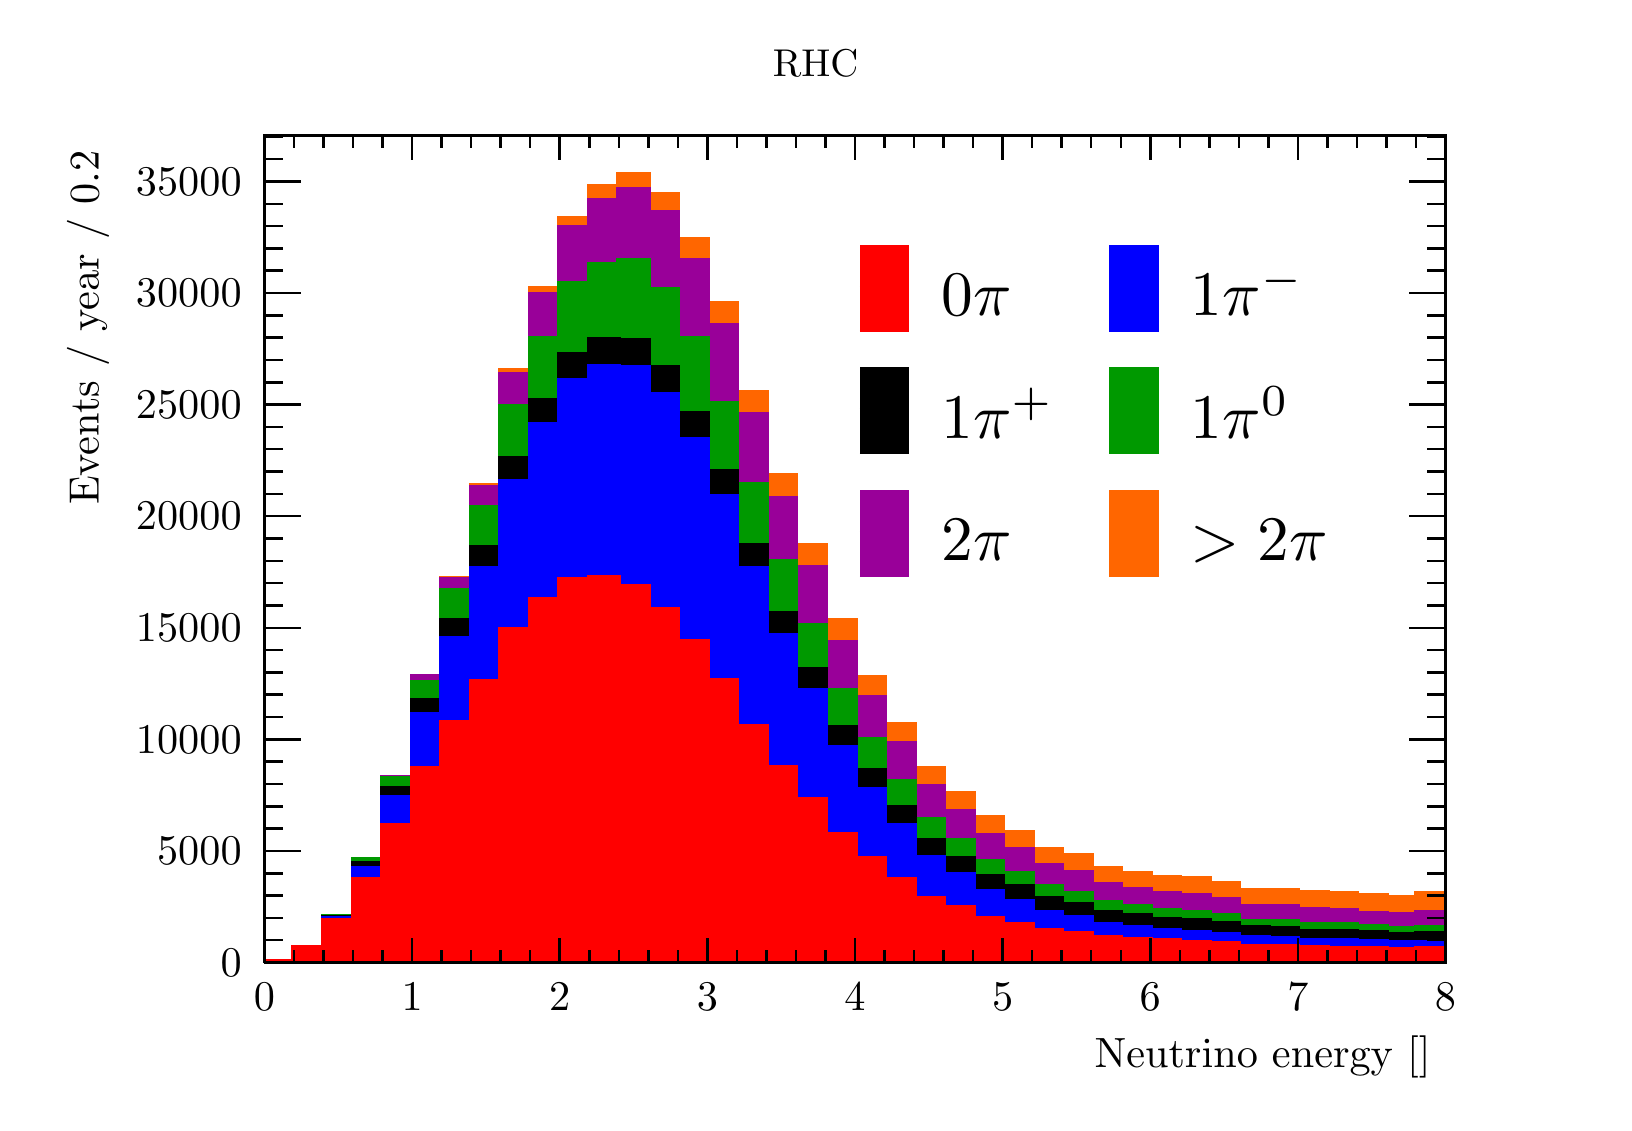
\begin{tikzpicture}
\pgfdeclareplotmark{cross} {
\pgfpathmoveto{\pgfpoint{-0.3\pgfplotmarksize}{\pgfplotmarksize}}
\pgfpathlineto{\pgfpoint{+0.3\pgfplotmarksize}{\pgfplotmarksize}}
\pgfpathlineto{\pgfpoint{+0.3\pgfplotmarksize}{0.3\pgfplotmarksize}}
\pgfpathlineto{\pgfpoint{+1\pgfplotmarksize}{0.3\pgfplotmarksize}}
\pgfpathlineto{\pgfpoint{+1\pgfplotmarksize}{-0.3\pgfplotmarksize}}
\pgfpathlineto{\pgfpoint{+0.3\pgfplotmarksize}{-0.3\pgfplotmarksize}}
\pgfpathlineto{\pgfpoint{+0.3\pgfplotmarksize}{-1.\pgfplotmarksize}}
\pgfpathlineto{\pgfpoint{-0.3\pgfplotmarksize}{-1.\pgfplotmarksize}}
\pgfpathlineto{\pgfpoint{-0.3\pgfplotmarksize}{-0.3\pgfplotmarksize}}
\pgfpathlineto{\pgfpoint{-1.\pgfplotmarksize}{-0.3\pgfplotmarksize}}
\pgfpathlineto{\pgfpoint{-1.\pgfplotmarksize}{0.3\pgfplotmarksize}}
\pgfpathlineto{\pgfpoint{-0.3\pgfplotmarksize}{0.3\pgfplotmarksize}}
\pgfpathclose
\pgfusepathqstroke
}
\pgfdeclareplotmark{cross*} {
\pgfpathmoveto{\pgfpoint{-0.3\pgfplotmarksize}{\pgfplotmarksize}}
\pgfpathlineto{\pgfpoint{+0.3\pgfplotmarksize}{\pgfplotmarksize}}
\pgfpathlineto{\pgfpoint{+0.3\pgfplotmarksize}{0.3\pgfplotmarksize}}
\pgfpathlineto{\pgfpoint{+1\pgfplotmarksize}{0.3\pgfplotmarksize}}
\pgfpathlineto{\pgfpoint{+1\pgfplotmarksize}{-0.3\pgfplotmarksize}}
\pgfpathlineto{\pgfpoint{+0.3\pgfplotmarksize}{-0.3\pgfplotmarksize}}
\pgfpathlineto{\pgfpoint{+0.3\pgfplotmarksize}{-1.\pgfplotmarksize}}
\pgfpathlineto{\pgfpoint{-0.3\pgfplotmarksize}{-1.\pgfplotmarksize}}
\pgfpathlineto{\pgfpoint{-0.3\pgfplotmarksize}{-0.3\pgfplotmarksize}}
\pgfpathlineto{\pgfpoint{-1.\pgfplotmarksize}{-0.3\pgfplotmarksize}}
\pgfpathlineto{\pgfpoint{-1.\pgfplotmarksize}{0.3\pgfplotmarksize}}
\pgfpathlineto{\pgfpoint{-0.3\pgfplotmarksize}{0.3\pgfplotmarksize}}
\pgfpathclose
\pgfusepathqfillstroke
}
\pgfdeclareplotmark{newstar} {
\pgfpathmoveto{\pgfqpoint{0pt}{\pgfplotmarksize}}
\pgfpathlineto{\pgfqpointpolar{44}{0.5\pgfplotmarksize}}
\pgfpathlineto{\pgfqpointpolar{18}{\pgfplotmarksize}}
\pgfpathlineto{\pgfqpointpolar{-20}{0.5\pgfplotmarksize}}
\pgfpathlineto{\pgfqpointpolar{-54}{\pgfplotmarksize}}
\pgfpathlineto{\pgfqpointpolar{-90}{0.5\pgfplotmarksize}}
\pgfpathlineto{\pgfqpointpolar{234}{\pgfplotmarksize}}
\pgfpathlineto{\pgfqpointpolar{198}{0.5\pgfplotmarksize}}
\pgfpathlineto{\pgfqpointpolar{162}{\pgfplotmarksize}}
\pgfpathlineto{\pgfqpointpolar{134}{0.5\pgfplotmarksize}}
\pgfpathclose
\pgfusepathqstroke
}
\pgfdeclareplotmark{newstar*} {
\pgfpathmoveto{\pgfqpoint{0pt}{\pgfplotmarksize}}
\pgfpathlineto{\pgfqpointpolar{44}{0.5\pgfplotmarksize}}
\pgfpathlineto{\pgfqpointpolar{18}{\pgfplotmarksize}}
\pgfpathlineto{\pgfqpointpolar{-20}{0.5\pgfplotmarksize}}
\pgfpathlineto{\pgfqpointpolar{-54}{\pgfplotmarksize}}
\pgfpathlineto{\pgfqpointpolar{-90}{0.5\pgfplotmarksize}}
\pgfpathlineto{\pgfqpointpolar{234}{\pgfplotmarksize}}
\pgfpathlineto{\pgfqpointpolar{198}{0.5\pgfplotmarksize}}
\pgfpathlineto{\pgfqpointpolar{162}{\pgfplotmarksize}}
\pgfpathlineto{\pgfqpointpolar{134}{0.5\pgfplotmarksize}}
\pgfpathclose
\pgfusepathqfillstroke
}
\definecolor{c}{rgb}{1,1,1};
\draw [color=c, fill=c] (0,0) rectangle (20,13.639);
\draw [color=c, fill=c] (3,1.77307) rectangle (18,12.2751);
\definecolor{c}{rgb}{0,0,0};
\draw [c,line width=0.9] (3,1.77307) -- (3,12.2751) -- (18,12.2751) -- (18,1.77307) -- (3,1.77307);
\definecolor{c}{rgb}{1,1,1};
\draw [color=c, fill=c] (3,1.77307) rectangle (18,12.2751);
\definecolor{c}{rgb}{0,0,0};
\draw [c,line width=0.9] (3,1.77307) -- (3,12.2751) -- (18,12.2751) -- (18,1.77307) -- (3,1.77307);
\draw [c,line width=0.9] (3,1.77307) -- (3.375,1.77307) -- (3.375,1.77307) -- (3.75,1.77307) -- (3.75,1.77307) -- (4.125,1.77307) -- (4.125,1.77307) -- (4.5,1.77307) -- (4.5,1.77307) -- (4.875,1.77307) -- (4.875,1.77307) -- (5.25,1.77307) --
 (5.25,1.77307) -- (5.625,1.77307) -- (5.625,1.77307) -- (6,1.77307) -- (6,1.77307) -- (6.375,1.77307) -- (6.375,1.77307) -- (6.75,1.77307) -- (6.75,1.77307) -- (7.125,1.77307) -- (7.125,1.77307) -- (7.5,1.77307) -- (7.5,1.77307) -- (7.875,1.77307)
 -- (7.875,1.77307) -- (8.25,1.77307) -- (8.25,1.77307) -- (8.625,1.77307) -- (8.625,1.77307) -- (9,1.77307) -- (9,1.77307) -- (9.375,1.77307) -- (9.375,1.77307) -- (9.75,1.77307) -- (9.75,1.77307) -- (10.125,1.77307) -- (10.125,1.77307) --
 (10.5,1.77307) -- (10.5,1.77307) -- (10.875,1.77307) -- (10.875,1.77307) -- (11.25,1.77307) -- (11.25,1.77307) -- (11.625,1.77307) -- (11.625,1.77307) -- (12,1.77307) -- (12,1.77307) -- (12.375,1.77307) -- (12.375,1.77307) -- (12.75,1.77307) --
 (12.75,1.77307) -- (13.125,1.77307) -- (13.125,1.77307) -- (13.5,1.77307) -- (13.5,1.77307) -- (13.875,1.77307) -- (13.875,1.77307) -- (14.25,1.77307) -- (14.25,1.77307) -- (14.625,1.77307) -- (14.625,1.77307) -- (15,1.77307) -- (15,1.77307) --
 (15.375,1.77307) -- (15.375,1.77307) -- (15.75,1.77307) -- (15.75,1.77307) -- (16.125,1.77307) -- (16.125,1.77307) -- (16.5,1.77307) -- (16.5,1.77307) -- (16.875,1.77307) -- (16.875,1.77307) -- (17.25,1.77307) -- (17.25,1.77307) -- (17.625,1.77307)
 -- (17.625,1.77307) -- (18,1.77307);
\draw [c,line width=0.9] (3,1.77307) -- (18,1.77307);
\draw [c,line width=0.9] (3,2.07994) -- (3,1.77307);
\draw [c,line width=0.9] (3.375,1.9265) -- (3.375,1.77307);
\draw [c,line width=0.9] (3.75,1.9265) -- (3.75,1.77307);
\draw [c,line width=0.9] (4.125,1.9265) -- (4.125,1.77307);
\draw [c,line width=0.9] (4.5,1.9265) -- (4.5,1.77307);
\draw [c,line width=0.9] (4.875,2.07994) -- (4.875,1.77307);
\draw [c,line width=0.9] (5.25,1.9265) -- (5.25,1.77307);
\draw [c,line width=0.9] (5.625,1.9265) -- (5.625,1.77307);
\draw [c,line width=0.9] (6,1.9265) -- (6,1.77307);
\draw [c,line width=0.9] (6.375,1.9265) -- (6.375,1.77307);
\draw [c,line width=0.9] (6.75,2.07994) -- (6.75,1.77307);
\draw [c,line width=0.9] (7.125,1.9265) -- (7.125,1.77307);
\draw [c,line width=0.9] (7.5,1.9265) -- (7.5,1.77307);
\draw [c,line width=0.9] (7.875,1.9265) -- (7.875,1.77307);
\draw [c,line width=0.9] (8.25,1.9265) -- (8.25,1.77307);
\draw [c,line width=0.9] (8.625,2.07994) -- (8.625,1.77307);
\draw [c,line width=0.9] (9,1.9265) -- (9,1.77307);
\draw [c,line width=0.9] (9.375,1.9265) -- (9.375,1.77307);
\draw [c,line width=0.9] (9.75,1.9265) -- (9.75,1.77307);
\draw [c,line width=0.9] (10.125,1.9265) -- (10.125,1.77307);
\draw [c,line width=0.9] (10.5,2.07994) -- (10.5,1.77307);
\draw [c,line width=0.9] (10.875,1.9265) -- (10.875,1.77307);
\draw [c,line width=0.9] (11.25,1.9265) -- (11.25,1.77307);
\draw [c,line width=0.9] (11.625,1.9265) -- (11.625,1.77307);
\draw [c,line width=0.9] (12,1.9265) -- (12,1.77307);
\draw [c,line width=0.9] (12.375,2.07994) -- (12.375,1.77307);
\draw [c,line width=0.9] (12.75,1.9265) -- (12.75,1.77307);
\draw [c,line width=0.9] (13.125,1.9265) -- (13.125,1.77307);
\draw [c,line width=0.9] (13.5,1.9265) -- (13.5,1.77307);
\draw [c,line width=0.9] (13.875,1.9265) -- (13.875,1.77307);
\draw [c,line width=0.9] (14.25,2.07994) -- (14.25,1.77307);
\draw [c,line width=0.9] (14.625,1.9265) -- (14.625,1.77307);
\draw [c,line width=0.9] (15,1.9265) -- (15,1.77307);
\draw [c,line width=0.9] (15.375,1.9265) -- (15.375,1.77307);
\draw [c,line width=0.9] (15.75,1.9265) -- (15.75,1.77307);
\draw [c,line width=0.9] (16.125,2.07994) -- (16.125,1.77307);
\draw [c,line width=0.9] (16.5,1.9265) -- (16.5,1.77307);
\draw [c,line width=0.9] (16.875,1.9265) -- (16.875,1.77307);
\draw [c,line width=0.9] (17.25,1.9265) -- (17.25,1.77307);
\draw [c,line width=0.9] (17.625,1.9265) -- (17.625,1.77307);
\draw [c,line width=0.9] (18,2.07994) -- (18,1.77307);
\draw [anchor=base] (3,1.15931) node[scale=1.52731, color=c, rotate=0]{0};
\draw [anchor=base] (4.875,1.15931) node[scale=1.52731, color=c, rotate=0]{1};
\draw [anchor=base] (6.75,1.15931) node[scale=1.52731, color=c, rotate=0]{2};
\draw [anchor=base] (8.625,1.15931) node[scale=1.52731, color=c, rotate=0]{3};
\draw [anchor=base] (10.5,1.15931) node[scale=1.52731, color=c, rotate=0]{4};
\draw [anchor=base] (12.375,1.15931) node[scale=1.52731, color=c, rotate=0]{5};
\draw [anchor=base] (14.25,1.15931) node[scale=1.52731, color=c, rotate=0]{6};
\draw [anchor=base] (16.125,1.15931) node[scale=1.52731, color=c, rotate=0]{7};
\draw [anchor=base] (18,1.15931) node[scale=1.52731, color=c, rotate=0]{8};
\draw [anchor= east] (18,0.572837) node[scale=1.52731, color=c, rotate=0]{ Neutrino energy [\si{\giga\electronvolt}] };
\draw [c,line width=0.9] (3,12.2751) -- (18,12.2751);
\draw [c,line width=0.9] (3,11.9682) -- (3,12.2751);
\draw [c,line width=0.9] (3.375,12.1216) -- (3.375,12.2751);
\draw [c,line width=0.9] (3.75,12.1216) -- (3.75,12.2751);
\draw [c,line width=0.9] (4.125,12.1216) -- (4.125,12.2751);
\draw [c,line width=0.9] (4.5,12.1216) -- (4.5,12.2751);
\draw [c,line width=0.9] (4.875,11.9682) -- (4.875,12.2751);
\draw [c,line width=0.9] (5.25,12.1216) -- (5.25,12.2751);
\draw [c,line width=0.9] (5.625,12.1216) -- (5.625,12.2751);
\draw [c,line width=0.9] (6,12.1216) -- (6,12.2751);
\draw [c,line width=0.9] (6.375,12.1216) -- (6.375,12.2751);
\draw [c,line width=0.9] (6.75,11.9682) -- (6.75,12.2751);
\draw [c,line width=0.9] (7.125,12.1216) -- (7.125,12.2751);
\draw [c,line width=0.9] (7.5,12.1216) -- (7.5,12.2751);
\draw [c,line width=0.9] (7.875,12.1216) -- (7.875,12.2751);
\draw [c,line width=0.9] (8.25,12.1216) -- (8.25,12.2751);
\draw [c,line width=0.9] (8.625,11.9682) -- (8.625,12.2751);
\draw [c,line width=0.9] (9,12.1216) -- (9,12.2751);
\draw [c,line width=0.9] (9.375,12.1216) -- (9.375,12.2751);
\draw [c,line width=0.9] (9.75,12.1216) -- (9.75,12.2751);
\draw [c,line width=0.9] (10.125,12.1216) -- (10.125,12.2751);
\draw [c,line width=0.9] (10.5,11.9682) -- (10.5,12.2751);
\draw [c,line width=0.9] (10.875,12.1216) -- (10.875,12.2751);
\draw [c,line width=0.9] (11.25,12.1216) -- (11.25,12.2751);
\draw [c,line width=0.9] (11.625,12.1216) -- (11.625,12.2751);
\draw [c,line width=0.9] (12,12.1216) -- (12,12.2751);
\draw [c,line width=0.9] (12.375,11.9682) -- (12.375,12.2751);
\draw [c,line width=0.9] (12.75,12.1216) -- (12.75,12.2751);
\draw [c,line width=0.9] (13.125,12.1216) -- (13.125,12.2751);
\draw [c,line width=0.9] (13.5,12.1216) -- (13.5,12.2751);
\draw [c,line width=0.9] (13.875,12.1216) -- (13.875,12.2751);
\draw [c,line width=0.9] (14.25,11.9682) -- (14.25,12.2751);
\draw [c,line width=0.9] (14.625,12.1216) -- (14.625,12.2751);
\draw [c,line width=0.9] (15,12.1216) -- (15,12.2751);
\draw [c,line width=0.9] (15.375,12.1216) -- (15.375,12.2751);
\draw [c,line width=0.9] (15.75,12.1216) -- (15.75,12.2751);
\draw [c,line width=0.9] (16.125,11.9682) -- (16.125,12.2751);
\draw [c,line width=0.9] (16.5,12.1216) -- (16.5,12.2751);
\draw [c,line width=0.9] (16.875,12.1216) -- (16.875,12.2751);
\draw [c,line width=0.9] (17.25,12.1216) -- (17.25,12.2751);
\draw [c,line width=0.9] (17.625,12.1216) -- (17.625,12.2751);
\draw [c,line width=0.9] (18,11.9682) -- (18,12.2751);
\draw [c,line width=0.9] (3,1.77307) -- (3,12.2751);
\draw [c,line width=0.9] (3.462,1.77307) -- (3,1.77307);
\draw [c,line width=0.9] (3.231,2.05649) -- (3,2.05649);
\draw [c,line width=0.9] (3.231,2.33992) -- (3,2.33992);
\draw [c,line width=0.9] (3.231,2.62335) -- (3,2.62335);
\draw [c,line width=0.9] (3.231,2.90677) -- (3,2.90677);
\draw [c,line width=0.9] (3.462,3.1902) -- (3,3.1902);
\draw [c,line width=0.9] (3.231,3.47362) -- (3,3.47362);
\draw [c,line width=0.9] (3.231,3.75705) -- (3,3.75705);
\draw [c,line width=0.9] (3.231,4.04048) -- (3,4.04048);
\draw [c,line width=0.9] (3.231,4.3239) -- (3,4.3239);
\draw [c,line width=0.9] (3.462,4.60733) -- (3,4.60733);
\draw [c,line width=0.9] (3.231,4.89076) -- (3,4.89076);
\draw [c,line width=0.9] (3.231,5.17418) -- (3,5.17418);
\draw [c,line width=0.9] (3.231,5.45761) -- (3,5.45761);
\draw [c,line width=0.9] (3.231,5.74104) -- (3,5.74104);
\draw [c,line width=0.9] (3.462,6.02446) -- (3,6.02446);
\draw [c,line width=0.9] (3.231,6.30789) -- (3,6.30789);
\draw [c,line width=0.9] (3.231,6.59131) -- (3,6.59131);
\draw [c,line width=0.9] (3.231,6.87474) -- (3,6.87474);
\draw [c,line width=0.9] (3.231,7.15817) -- (3,7.15817);
\draw [c,line width=0.9] (3.462,7.44159) -- (3,7.44159);
\draw [c,line width=0.9] (3.231,7.72502) -- (3,7.72502);
\draw [c,line width=0.9] (3.231,8.00845) -- (3,8.00845);
\draw [c,line width=0.9] (3.231,8.29187) -- (3,8.29187);
\draw [c,line width=0.9] (3.231,8.5753) -- (3,8.5753);
\draw [c,line width=0.9] (3.462,8.85873) -- (3,8.85873);
\draw [c,line width=0.9] (3.231,9.14215) -- (3,9.14215);
\draw [c,line width=0.9] (3.231,9.42558) -- (3,9.42558);
\draw [c,line width=0.9] (3.231,9.70901) -- (3,9.70901);
\draw [c,line width=0.9] (3.231,9.99243) -- (3,9.99243);
\draw [c,line width=0.9] (3.462,10.2759) -- (3,10.2759);
\draw [c,line width=0.9] (3.231,10.5593) -- (3,10.5593);
\draw [c,line width=0.9] (3.231,10.8427) -- (3,10.8427);
\draw [c,line width=0.9] (3.231,11.1261) -- (3,11.1261);
\draw [c,line width=0.9] (3.231,11.4096) -- (3,11.4096);
\draw [c,line width=0.9] (3.462,11.693) -- (3,11.693);
\draw [c,line width=0.9] (3.462,11.693) -- (3,11.693);
\draw [c,line width=0.9] (3.231,11.9764) -- (3,11.9764);
\draw [c,line width=0.9] (3.231,12.2598) -- (3,12.2598);
\draw [anchor= east] (2.9,1.77307) node[scale=1.52731, color=c, rotate=0]{0};
\draw [anchor= east] (2.9,3.1902) node[scale=1.52731, color=c, rotate=0]{5000};
\draw [anchor= east] (2.9,4.60733) node[scale=1.52731, color=c, rotate=0]{10000};
\draw [anchor= east] (2.9,6.02446) node[scale=1.52731, color=c, rotate=0]{15000};
\draw [anchor= east] (2.9,7.44159) node[scale=1.52731, color=c, rotate=0]{20000};
\draw [anchor= east] (2.9,8.85873) node[scale=1.52731, color=c, rotate=0]{25000};
\draw [anchor= east] (2.9,10.2759) node[scale=1.52731, color=c, rotate=0]{30000};
\draw [anchor= east] (2.9,11.693) node[scale=1.52731, color=c, rotate=0]{35000};
\draw [anchor= east] (0.76,12.2751) node[scale=1.52731, color=c, rotate=90]{ Events / year / \SI{0.2}{\giga\electronvolt} };
\draw [c,line width=0.9] (18,1.77307) -- (18,12.2751);
\draw [c,line width=0.9] (17.538,1.77307) -- (18,1.77307);
\draw [c,line width=0.9] (17.769,2.05649) -- (18,2.05649);
\draw [c,line width=0.9] (17.769,2.33992) -- (18,2.33992);
\draw [c,line width=0.9] (17.769,2.62335) -- (18,2.62335);
\draw [c,line width=0.9] (17.769,2.90677) -- (18,2.90677);
\draw [c,line width=0.9] (17.538,3.1902) -- (18,3.1902);
\draw [c,line width=0.9] (17.769,3.47362) -- (18,3.47362);
\draw [c,line width=0.9] (17.769,3.75705) -- (18,3.75705);
\draw [c,line width=0.9] (17.769,4.04048) -- (18,4.04048);
\draw [c,line width=0.9] (17.769,4.3239) -- (18,4.3239);
\draw [c,line width=0.9] (17.538,4.60733) -- (18,4.60733);
\draw [c,line width=0.9] (17.769,4.89076) -- (18,4.89076);
\draw [c,line width=0.9] (17.769,5.17418) -- (18,5.17418);
\draw [c,line width=0.9] (17.769,5.45761) -- (18,5.45761);
\draw [c,line width=0.9] (17.769,5.74104) -- (18,5.74104);
\draw [c,line width=0.9] (17.538,6.02446) -- (18,6.02446);
\draw [c,line width=0.9] (17.769,6.30789) -- (18,6.30789);
\draw [c,line width=0.9] (17.769,6.59131) -- (18,6.59131);
\draw [c,line width=0.9] (17.769,6.87474) -- (18,6.87474);
\draw [c,line width=0.9] (17.769,7.15817) -- (18,7.15817);
\draw [c,line width=0.9] (17.538,7.44159) -- (18,7.44159);
\draw [c,line width=0.9] (17.769,7.72502) -- (18,7.72502);
\draw [c,line width=0.9] (17.769,8.00845) -- (18,8.00845);
\draw [c,line width=0.9] (17.769,8.29187) -- (18,8.29187);
\draw [c,line width=0.9] (17.769,8.5753) -- (18,8.5753);
\draw [c,line width=0.9] (17.538,8.85873) -- (18,8.85873);
\draw [c,line width=0.9] (17.769,9.14215) -- (18,9.14215);
\draw [c,line width=0.9] (17.769,9.42558) -- (18,9.42558);
\draw [c,line width=0.9] (17.769,9.70901) -- (18,9.70901);
\draw [c,line width=0.9] (17.769,9.99243) -- (18,9.99243);
\draw [c,line width=0.9] (17.538,10.2759) -- (18,10.2759);
\draw [c,line width=0.9] (17.769,10.5593) -- (18,10.5593);
\draw [c,line width=0.9] (17.769,10.8427) -- (18,10.8427);
\draw [c,line width=0.9] (17.769,11.1261) -- (18,11.1261);
\draw [c,line width=0.9] (17.769,11.4096) -- (18,11.4096);
\draw [c,line width=0.9] (17.538,11.693) -- (18,11.693);
\draw [c,line width=0.9] (17.538,11.693) -- (18,11.693);
\draw [c,line width=0.9] (17.769,11.9764) -- (18,11.9764);
\draw [c,line width=0.9] (17.769,12.2598) -- (18,12.2598);
\definecolor{c}{rgb}{1,0.4,0};
\draw [c, fill=c] (3,1.77307) -- (3,1.7815) -- (3.375,1.7815) -- (3.375,1.96202) -- (3.75,1.96202) -- (3.75,2.35282) -- (4.125,2.35282) -- (4.125,3.08114) -- (4.5,3.08114) -- (4.5,4.12375) -- (4.875,4.12375) -- (4.875,5.40336) -- (5.25,5.40336) --
 (5.25,6.64876) -- (5.625,6.64876) -- (5.625,7.8288) -- (6,7.8288) -- (6,9.28607) -- (6.375,9.28607) -- (6.375,10.3376) -- (6.75,10.3376) -- (6.75,11.221) -- (7.125,11.221) -- (7.125,11.624) -- (7.5,11.624) -- (7.5,11.775) -- (7.875,11.775) --
 (7.875,11.5305) -- (8.25,11.5305) -- (8.25,10.9544) -- (8.625,10.9544) -- (8.625,10.138) -- (9,10.138) -- (9,9.01345) -- (9.375,9.01345) -- (9.375,7.95684) -- (9.75,7.95684) -- (9.75,7.06708) -- (10.125,7.06708) -- (10.125,6.11084) -- (10.5,6.11084)
 -- (10.5,5.39843) -- (10.875,5.39843) -- (10.875,4.79926) -- (11.25,4.79926) -- (11.25,4.23827) -- (11.625,4.23827) -- (11.625,3.92255) -- (12,3.92255) -- (12,3.60921) -- (12.375,3.60921) -- (12.375,3.42486) -- (12.75,3.42486) -- (12.75,3.21332) --
 (13.125,3.21332) -- (13.125,3.13697) -- (13.5,3.13697) -- (13.5,2.9636) -- (13.875,2.9636) -- (13.875,2.90061) -- (14.25,2.90061) -- (14.25,2.85655) -- (14.625,2.85655) -- (14.625,2.83572) -- (15,2.83572) -- (15,2.78053) -- (15.375,2.78053) --
 (15.375,2.69352) -- (15.75,2.69352) -- (15.75,2.6905) -- (16.125,2.6905) -- (16.125,2.65885) -- (16.5,2.65885) -- (16.5,2.64612) -- (16.875,2.64612) -- (16.875,2.62799) -- (17.25,2.62799) -- (17.25,2.59379) -- (17.625,2.59379) -- (17.625,2.65169) --
 (18,2.65169) -- (18,1.77307);
\draw [c,line width=1.8] (3,1.7815) -- (3.375,1.7815) -- (3.375,1.96202) -- (3.75,1.96202) -- (3.75,2.35282) -- (4.125,2.35282) -- (4.125,3.08114) -- (4.5,3.08114) -- (4.5,4.12375) -- (4.875,4.12375) -- (4.875,5.40336) -- (5.25,5.40336) --
 (5.25,6.64876) -- (5.625,6.64876) -- (5.625,7.8288) -- (6,7.8288) -- (6,9.28607) -- (6.375,9.28607) -- (6.375,10.3376) -- (6.75,10.3376) -- (6.75,11.221) -- (7.125,11.221) -- (7.125,11.624) -- (7.5,11.624) -- (7.5,11.775) -- (7.875,11.775) --
 (7.875,11.5305) -- (8.25,11.5305) -- (8.25,10.9544) -- (8.625,10.9544) -- (8.625,10.138) -- (9,10.138) -- (9,9.01345) -- (9.375,9.01345) -- (9.375,7.95684) -- (9.75,7.95684) -- (9.75,7.06708) -- (10.125,7.06708) -- (10.125,6.11084) -- (10.5,6.11084)
 -- (10.5,5.39843) -- (10.875,5.39843) -- (10.875,4.79926) -- (11.25,4.79926) -- (11.25,4.23827) -- (11.625,4.23827) -- (11.625,3.92255) -- (12,3.92255) -- (12,3.60921) -- (12.375,3.60921) -- (12.375,3.42486) -- (12.75,3.42486) -- (12.75,3.21332) --
 (13.125,3.21332) -- (13.125,3.13697) -- (13.5,3.13697) -- (13.5,2.9636) -- (13.875,2.9636) -- (13.875,2.90061) -- (14.25,2.90061) -- (14.25,2.85655) -- (14.625,2.85655) -- (14.625,2.83572) -- (15,2.83572) -- (15,2.78053) -- (15.375,2.78053) --
 (15.375,2.69352) -- (15.75,2.69352) -- (15.75,2.6905) -- (16.125,2.6905) -- (16.125,2.65885) -- (16.5,2.65885) -- (16.5,2.64612) -- (16.875,2.64612) -- (16.875,2.62799) -- (17.25,2.62799) -- (17.25,2.59379) -- (17.625,2.59379) -- (17.625,2.65169) --
 (18,2.65169);
\definecolor{c}{rgb}{0.999,0.999,0.999};
\draw [c, fill=c] (3,1.77307) -- (3,1.7815) -- (3.375,1.7815) -- (3.375,1.96202) -- (3.75,1.96202) -- (3.75,2.35282) -- (4.125,2.35282) -- (4.125,3.08114) -- (4.5,3.08114) -- (4.5,4.12328) -- (4.875,4.12328) -- (4.875,5.40049) -- (5.25,5.40049) --
 (5.25,6.64002) -- (5.625,6.64002) -- (5.625,7.80478) -- (6,7.80478) -- (6,9.23851) -- (6.375,9.23851) -- (6.375,10.2601) -- (6.75,10.2601) -- (6.75,11.1093) -- (7.125,11.1093) -- (7.125,11.4558) -- (7.5,11.4558) -- (7.5,11.5846) -- (7.875,11.5846)
 -- (7.875,11.2953) -- (8.25,11.2953) -- (8.25,10.6901) -- (8.625,10.6901) -- (8.625,9.85899) -- (9,9.85899) -- (9,8.72858) -- (9.375,8.72858) -- (9.375,7.66768) -- (9.75,7.66768) -- (9.75,6.78873) -- (10.125,6.78873) -- (10.125,5.83965) --
 (10.5,5.83965) -- (10.5,5.14298) -- (10.875,5.14298) -- (10.875,4.55511) -- (11.25,4.55511) -- (11.25,4.00764) -- (11.625,4.00764) -- (11.625,3.69223) -- (12,3.69223) -- (12,3.39305) -- (12.375,3.39305) -- (12.375,3.20918) -- (12.75,3.20918) --
 (12.75,3.01036) -- (13.125,3.01036) -- (13.125,2.91525) -- (13.5,2.91525) -- (13.5,2.7608) -- (13.875,2.7608) -- (13.875,2.7045) -- (14.25,2.7045) -- (14.25,2.64501) -- (14.625,2.64501) -- (14.625,2.61924) -- (15,2.61924) -- (15,2.56819) --
 (15.375,2.56819) -- (15.375,2.48611) -- (15.75,2.48611) -- (15.75,2.4823) -- (16.125,2.4823) -- (16.125,2.44317) -- (16.5,2.44317) -- (16.5,2.43426) -- (16.875,2.43426) -- (16.875,2.39863) -- (17.25,2.39863) -- (17.25,2.37907) -- (17.625,2.37907) --
 (17.625,2.40929) -- (18,2.40929) -- (18,1.77307);
\definecolor{c}{rgb}{0.6,0,0.6};
\draw [c,line width=1.8] (3,1.7815) -- (3.375,1.7815) -- (3.375,1.96202) -- (3.75,1.96202) -- (3.75,2.35282) -- (4.125,2.35282) -- (4.125,3.08114) -- (4.5,3.08114) -- (4.5,4.12328) -- (4.875,4.12328) -- (4.875,5.40049) -- (5.25,5.40049) --
 (5.25,6.64002) -- (5.625,6.64002) -- (5.625,7.80478) -- (6,7.80478) -- (6,9.23851) -- (6.375,9.23851) -- (6.375,10.2601) -- (6.75,10.2601) -- (6.75,11.1093) -- (7.125,11.1093) -- (7.125,11.4558) -- (7.5,11.4558) -- (7.5,11.5846) -- (7.875,11.5846)
 -- (7.875,11.2953) -- (8.25,11.2953) -- (8.25,10.6901) -- (8.625,10.6901) -- (8.625,9.85899) -- (9,9.85899) -- (9,8.72858) -- (9.375,8.72858) -- (9.375,7.66768) -- (9.75,7.66768) -- (9.75,6.78873) -- (10.125,6.78873) -- (10.125,5.83965) --
 (10.5,5.83965) -- (10.5,5.14298) -- (10.875,5.14298) -- (10.875,4.55511) -- (11.25,4.55511) -- (11.25,4.00764) -- (11.625,4.00764) -- (11.625,3.69223) -- (12,3.69223) -- (12,3.39305) -- (12.375,3.39305) -- (12.375,3.20918) -- (12.75,3.20918) --
 (12.75,3.01036) -- (13.125,3.01036) -- (13.125,2.91525) -- (13.5,2.91525) -- (13.5,2.7608) -- (13.875,2.7608) -- (13.875,2.7045) -- (14.25,2.7045) -- (14.25,2.64501) -- (14.625,2.64501) -- (14.625,2.61924) -- (15,2.61924) -- (15,2.56819) --
 (15.375,2.56819) -- (15.375,2.48611) -- (15.75,2.48611) -- (15.75,2.4823) -- (16.125,2.4823) -- (16.125,2.44317) -- (16.5,2.44317) -- (16.5,2.43426) -- (16.875,2.43426) -- (16.875,2.39863) -- (17.25,2.39863) -- (17.25,2.37907) -- (17.625,2.37907) --
 (17.625,2.40929) -- (18,2.40929);
\draw [c,line width=1.8] (3,1.7815) -- (3.375,1.7815) -- (3.375,1.96202) -- (3.75,1.96202) -- (3.75,2.35282) -- (4.125,2.35282) -- (4.125,3.08114) -- (4.5,3.08114) -- (4.5,4.12328) -- (4.875,4.12328) -- (4.875,5.40049) -- (5.25,5.40049) --
 (5.25,6.64002) -- (5.625,6.64002) -- (5.625,7.80478) -- (6,7.80478) -- (6,9.23851) -- (6.375,9.23851) -- (6.375,10.2601) -- (6.75,10.2601) -- (6.75,11.1093) -- (7.125,11.1093) -- (7.125,11.4558) -- (7.5,11.4558) -- (7.5,11.5846) -- (7.875,11.5846)
 -- (7.875,11.2953) -- (8.25,11.2953) -- (8.25,10.6901) -- (8.625,10.6901) -- (8.625,9.85899) -- (9,9.85899) -- (9,8.72858) -- (9.375,8.72858) -- (9.375,7.66768) -- (9.75,7.66768) -- (9.75,6.78873) -- (10.125,6.78873) -- (10.125,5.83965) --
 (10.5,5.83965) -- (10.5,5.14298) -- (10.875,5.14298) -- (10.875,4.55511) -- (11.25,4.55511) -- (11.25,4.00764) -- (11.625,4.00764) -- (11.625,3.69223) -- (12,3.69223) -- (12,3.39305) -- (12.375,3.39305) -- (12.375,3.20918) -- (12.75,3.20918) --
 (12.75,3.01036) -- (13.125,3.01036) -- (13.125,2.91525) -- (13.5,2.91525) -- (13.5,2.7608) -- (13.875,2.7608) -- (13.875,2.7045) -- (14.25,2.7045) -- (14.25,2.64501) -- (14.625,2.64501) -- (14.625,2.61924) -- (15,2.61924) -- (15,2.56819) --
 (15.375,2.56819) -- (15.375,2.48611) -- (15.75,2.48611) -- (15.75,2.4823) -- (16.125,2.4823) -- (16.125,2.44317) -- (16.5,2.44317) -- (16.5,2.43426) -- (16.875,2.43426) -- (16.875,2.39863) -- (17.25,2.39863) -- (17.25,2.37907) -- (17.625,2.37907) --
 (17.625,2.40929) -- (18,2.40929);
\draw [c, fill=c] (3,1.77307) -- (3,1.7815) -- (3.375,1.7815) -- (3.375,1.96202) -- (3.75,1.96202) -- (3.75,2.35282) -- (4.125,2.35282) -- (4.125,3.08114) -- (4.5,3.08114) -- (4.5,4.12328) -- (4.875,4.12328) -- (4.875,5.40049) -- (5.25,5.40049) --
 (5.25,6.64002) -- (5.625,6.64002) -- (5.625,7.80478) -- (6,7.80478) -- (6,9.23851) -- (6.375,9.23851) -- (6.375,10.2601) -- (6.75,10.2601) -- (6.75,11.1093) -- (7.125,11.1093) -- (7.125,11.4558) -- (7.5,11.4558) -- (7.5,11.5846) -- (7.875,11.5846)
 -- (7.875,11.2953) -- (8.25,11.2953) -- (8.25,10.6901) -- (8.625,10.6901) -- (8.625,9.85899) -- (9,9.85899) -- (9,8.72858) -- (9.375,8.72858) -- (9.375,7.66768) -- (9.75,7.66768) -- (9.75,6.78873) -- (10.125,6.78873) -- (10.125,5.83965) --
 (10.5,5.83965) -- (10.5,5.14298) -- (10.875,5.14298) -- (10.875,4.55511) -- (11.25,4.55511) -- (11.25,4.00764) -- (11.625,4.00764) -- (11.625,3.69223) -- (12,3.69223) -- (12,3.39305) -- (12.375,3.39305) -- (12.375,3.20918) -- (12.75,3.20918) --
 (12.75,3.01036) -- (13.125,3.01036) -- (13.125,2.91525) -- (13.5,2.91525) -- (13.5,2.7608) -- (13.875,2.7608) -- (13.875,2.7045) -- (14.25,2.7045) -- (14.25,2.64501) -- (14.625,2.64501) -- (14.625,2.61924) -- (15,2.61924) -- (15,2.56819) --
 (15.375,2.56819) -- (15.375,2.48611) -- (15.75,2.48611) -- (15.75,2.4823) -- (16.125,2.4823) -- (16.125,2.44317) -- (16.5,2.44317) -- (16.5,2.43426) -- (16.875,2.43426) -- (16.875,2.39863) -- (17.25,2.39863) -- (17.25,2.37907) -- (17.625,2.37907) --
 (17.625,2.40929) -- (18,2.40929) -- (18,1.77307);
\draw [c,line width=1.8] (3,1.7815) -- (3.375,1.7815) -- (3.375,1.96202) -- (3.75,1.96202) -- (3.75,2.35282) -- (4.125,2.35282) -- (4.125,3.08114) -- (4.5,3.08114) -- (4.5,4.12328) -- (4.875,4.12328) -- (4.875,5.40049) -- (5.25,5.40049) --
 (5.25,6.64002) -- (5.625,6.64002) -- (5.625,7.80478) -- (6,7.80478) -- (6,9.23851) -- (6.375,9.23851) -- (6.375,10.2601) -- (6.75,10.2601) -- (6.75,11.1093) -- (7.125,11.1093) -- (7.125,11.4558) -- (7.5,11.4558) -- (7.5,11.5846) -- (7.875,11.5846)
 -- (7.875,11.2953) -- (8.25,11.2953) -- (8.25,10.6901) -- (8.625,10.6901) -- (8.625,9.85899) -- (9,9.85899) -- (9,8.72858) -- (9.375,8.72858) -- (9.375,7.66768) -- (9.75,7.66768) -- (9.75,6.78873) -- (10.125,6.78873) -- (10.125,5.83965) --
 (10.5,5.83965) -- (10.5,5.14298) -- (10.875,5.14298) -- (10.875,4.55511) -- (11.25,4.55511) -- (11.25,4.00764) -- (11.625,4.00764) -- (11.625,3.69223) -- (12,3.69223) -- (12,3.39305) -- (12.375,3.39305) -- (12.375,3.20918) -- (12.75,3.20918) --
 (12.75,3.01036) -- (13.125,3.01036) -- (13.125,2.91525) -- (13.5,2.91525) -- (13.5,2.7608) -- (13.875,2.7608) -- (13.875,2.7045) -- (14.25,2.7045) -- (14.25,2.64501) -- (14.625,2.64501) -- (14.625,2.61924) -- (15,2.61924) -- (15,2.56819) --
 (15.375,2.56819) -- (15.375,2.48611) -- (15.75,2.48611) -- (15.75,2.4823) -- (16.125,2.4823) -- (16.125,2.44317) -- (16.5,2.44317) -- (16.5,2.43426) -- (16.875,2.43426) -- (16.875,2.39863) -- (17.25,2.39863) -- (17.25,2.37907) -- (17.625,2.37907) --
 (17.625,2.40929) -- (18,2.40929);
\definecolor{c}{rgb}{0.999,0.999,0.999};
\draw [c, fill=c] (3,1.77307) -- (3,1.7815) -- (3.375,1.7815) -- (3.375,1.96202) -- (3.75,1.96202) -- (3.75,2.35267) -- (4.125,2.35267) -- (4.125,3.07923) -- (4.5,3.07923) -- (4.5,4.10848) -- (4.875,4.10848) -- (4.875,5.33592) -- (5.25,5.33592) --
 (5.25,6.49559) -- (5.625,6.49559) -- (5.625,7.54934) -- (6,7.54934) -- (6,8.83308) -- (6.375,8.83308) -- (6.375,9.70025) -- (6.75,9.70025) -- (6.75,10.4023) -- (7.125,10.4023) -- (7.125,10.6382) -- (7.5,10.6382) -- (7.5,10.6848) -- (7.875,10.6848)
 -- (7.875,10.3242) -- (8.25,10.3242) -- (8.25,9.7028) -- (8.625,9.7028) -- (8.625,8.86696) -- (9,8.86696) -- (9,7.84646) -- (9.375,7.84646) -- (9.375,6.86413) -- (9.75,6.86413) -- (9.75,6.05215) -- (10.125,6.05215) -- (10.125,5.22919) --
 (10.5,5.22919) -- (10.5,4.60235) -- (10.875,4.60235) -- (10.875,4.07333) -- (11.25,4.07333) -- (11.25,3.59266) -- (11.625,3.59266) -- (11.625,3.3202) -- (12,3.3202) -- (12,3.05299) -- (12.375,3.05299) -- (12.375,2.90014) -- (12.75,2.90014) --
 (12.75,2.74315) -- (13.125,2.74315) -- (13.125,2.65551) -- (13.5,2.65551) -- (13.5,2.53097) -- (13.875,2.53097) -- (13.875,2.4823) -- (14.25,2.4823) -- (14.25,2.42997) -- (14.625,2.42997) -- (14.625,2.41024) -- (15,2.41024) -- (15,2.36491) --
 (15.375,2.36491) -- (15.375,2.29652) -- (15.75,2.29652) -- (15.75,2.29143) -- (16.125,2.29143) -- (16.125,2.26184) -- (16.5,2.26184) -- (16.5,2.25564) -- (16.875,2.25564) -- (16.875,2.22526) -- (17.25,2.22526) -- (17.25,2.21015) -- (17.625,2.21015)
 -- (17.625,2.22113) -- (18,2.22113) -- (18,1.77307);
\definecolor{c}{rgb}{0,0.6,0};
\draw [c,line width=1.8] (3,1.7815) -- (3.375,1.7815) -- (3.375,1.96202) -- (3.75,1.96202) -- (3.75,2.35267) -- (4.125,2.35267) -- (4.125,3.07923) -- (4.5,3.07923) -- (4.5,4.10848) -- (4.875,4.10848) -- (4.875,5.33592) -- (5.25,5.33592) --
 (5.25,6.49559) -- (5.625,6.49559) -- (5.625,7.54934) -- (6,7.54934) -- (6,8.83308) -- (6.375,8.83308) -- (6.375,9.70025) -- (6.75,9.70025) -- (6.75,10.4023) -- (7.125,10.4023) -- (7.125,10.6382) -- (7.5,10.6382) -- (7.5,10.6848) -- (7.875,10.6848)
 -- (7.875,10.3242) -- (8.25,10.3242) -- (8.25,9.7028) -- (8.625,9.7028) -- (8.625,8.86696) -- (9,8.86696) -- (9,7.84646) -- (9.375,7.84646) -- (9.375,6.86413) -- (9.75,6.86413) -- (9.75,6.05215) -- (10.125,6.05215) -- (10.125,5.22919) --
 (10.5,5.22919) -- (10.5,4.60235) -- (10.875,4.60235) -- (10.875,4.07333) -- (11.25,4.07333) -- (11.25,3.59266) -- (11.625,3.59266) -- (11.625,3.3202) -- (12,3.3202) -- (12,3.05299) -- (12.375,3.05299) -- (12.375,2.90014) -- (12.75,2.90014) --
 (12.75,2.74315) -- (13.125,2.74315) -- (13.125,2.65551) -- (13.5,2.65551) -- (13.5,2.53097) -- (13.875,2.53097) -- (13.875,2.4823) -- (14.25,2.4823) -- (14.25,2.42997) -- (14.625,2.42997) -- (14.625,2.41024) -- (15,2.41024) -- (15,2.36491) --
 (15.375,2.36491) -- (15.375,2.29652) -- (15.75,2.29652) -- (15.75,2.29143) -- (16.125,2.29143) -- (16.125,2.26184) -- (16.5,2.26184) -- (16.5,2.25564) -- (16.875,2.25564) -- (16.875,2.22526) -- (17.25,2.22526) -- (17.25,2.21015) -- (17.625,2.21015)
 -- (17.625,2.22113) -- (18,2.22113);
\draw [c,line width=1.8] (3,1.7815) -- (3.375,1.7815) -- (3.375,1.96202) -- (3.75,1.96202) -- (3.75,2.35267) -- (4.125,2.35267) -- (4.125,3.07923) -- (4.5,3.07923) -- (4.5,4.10848) -- (4.875,4.10848) -- (4.875,5.33592) -- (5.25,5.33592) --
 (5.25,6.49559) -- (5.625,6.49559) -- (5.625,7.54934) -- (6,7.54934) -- (6,8.83308) -- (6.375,8.83308) -- (6.375,9.70025) -- (6.75,9.70025) -- (6.75,10.4023) -- (7.125,10.4023) -- (7.125,10.6382) -- (7.5,10.6382) -- (7.5,10.6848) -- (7.875,10.6848)
 -- (7.875,10.3242) -- (8.25,10.3242) -- (8.25,9.7028) -- (8.625,9.7028) -- (8.625,8.86696) -- (9,8.86696) -- (9,7.84646) -- (9.375,7.84646) -- (9.375,6.86413) -- (9.75,6.86413) -- (9.75,6.05215) -- (10.125,6.05215) -- (10.125,5.22919) --
 (10.5,5.22919) -- (10.5,4.60235) -- (10.875,4.60235) -- (10.875,4.07333) -- (11.25,4.07333) -- (11.25,3.59266) -- (11.625,3.59266) -- (11.625,3.3202) -- (12,3.3202) -- (12,3.05299) -- (12.375,3.05299) -- (12.375,2.90014) -- (12.75,2.90014) --
 (12.75,2.74315) -- (13.125,2.74315) -- (13.125,2.65551) -- (13.5,2.65551) -- (13.5,2.53097) -- (13.875,2.53097) -- (13.875,2.4823) -- (14.25,2.4823) -- (14.25,2.42997) -- (14.625,2.42997) -- (14.625,2.41024) -- (15,2.41024) -- (15,2.36491) --
 (15.375,2.36491) -- (15.375,2.29652) -- (15.75,2.29652) -- (15.75,2.29143) -- (16.125,2.29143) -- (16.125,2.26184) -- (16.5,2.26184) -- (16.5,2.25564) -- (16.875,2.25564) -- (16.875,2.22526) -- (17.25,2.22526) -- (17.25,2.21015) -- (17.625,2.21015)
 -- (17.625,2.22113) -- (18,2.22113);
\draw [c, fill=c] (3,1.77307) -- (3,1.7815) -- (3.375,1.7815) -- (3.375,1.96202) -- (3.75,1.96202) -- (3.75,2.35267) -- (4.125,2.35267) -- (4.125,3.07923) -- (4.5,3.07923) -- (4.5,4.10848) -- (4.875,4.10848) -- (4.875,5.33592) -- (5.25,5.33592) --
 (5.25,6.49559) -- (5.625,6.49559) -- (5.625,7.54934) -- (6,7.54934) -- (6,8.83308) -- (6.375,8.83308) -- (6.375,9.70025) -- (6.75,9.70025) -- (6.75,10.4023) -- (7.125,10.4023) -- (7.125,10.6382) -- (7.5,10.6382) -- (7.5,10.6848) -- (7.875,10.6848)
 -- (7.875,10.3242) -- (8.25,10.3242) -- (8.25,9.7028) -- (8.625,9.7028) -- (8.625,8.86696) -- (9,8.86696) -- (9,7.84646) -- (9.375,7.84646) -- (9.375,6.86413) -- (9.75,6.86413) -- (9.75,6.05215) -- (10.125,6.05215) -- (10.125,5.22919) --
 (10.5,5.22919) -- (10.5,4.60235) -- (10.875,4.60235) -- (10.875,4.07333) -- (11.25,4.07333) -- (11.25,3.59266) -- (11.625,3.59266) -- (11.625,3.3202) -- (12,3.3202) -- (12,3.05299) -- (12.375,3.05299) -- (12.375,2.90014) -- (12.75,2.90014) --
 (12.75,2.74315) -- (13.125,2.74315) -- (13.125,2.65551) -- (13.5,2.65551) -- (13.5,2.53097) -- (13.875,2.53097) -- (13.875,2.4823) -- (14.25,2.4823) -- (14.25,2.42997) -- (14.625,2.42997) -- (14.625,2.41024) -- (15,2.41024) -- (15,2.36491) --
 (15.375,2.36491) -- (15.375,2.29652) -- (15.75,2.29652) -- (15.75,2.29143) -- (16.125,2.29143) -- (16.125,2.26184) -- (16.5,2.26184) -- (16.5,2.25564) -- (16.875,2.25564) -- (16.875,2.22526) -- (17.25,2.22526) -- (17.25,2.21015) -- (17.625,2.21015)
 -- (17.625,2.22113) -- (18,2.22113) -- (18,1.77307);
\draw [c,line width=1.8] (3,1.7815) -- (3.375,1.7815) -- (3.375,1.96202) -- (3.75,1.96202) -- (3.75,2.35267) -- (4.125,2.35267) -- (4.125,3.07923) -- (4.5,3.07923) -- (4.5,4.10848) -- (4.875,4.10848) -- (4.875,5.33592) -- (5.25,5.33592) --
 (5.25,6.49559) -- (5.625,6.49559) -- (5.625,7.54934) -- (6,7.54934) -- (6,8.83308) -- (6.375,8.83308) -- (6.375,9.70025) -- (6.75,9.70025) -- (6.75,10.4023) -- (7.125,10.4023) -- (7.125,10.6382) -- (7.5,10.6382) -- (7.5,10.6848) -- (7.875,10.6848)
 -- (7.875,10.3242) -- (8.25,10.3242) -- (8.25,9.7028) -- (8.625,9.7028) -- (8.625,8.86696) -- (9,8.86696) -- (9,7.84646) -- (9.375,7.84646) -- (9.375,6.86413) -- (9.75,6.86413) -- (9.75,6.05215) -- (10.125,6.05215) -- (10.125,5.22919) --
 (10.5,5.22919) -- (10.5,4.60235) -- (10.875,4.60235) -- (10.875,4.07333) -- (11.25,4.07333) -- (11.25,3.59266) -- (11.625,3.59266) -- (11.625,3.3202) -- (12,3.3202) -- (12,3.05299) -- (12.375,3.05299) -- (12.375,2.90014) -- (12.75,2.90014) --
 (12.75,2.74315) -- (13.125,2.74315) -- (13.125,2.65551) -- (13.5,2.65551) -- (13.5,2.53097) -- (13.875,2.53097) -- (13.875,2.4823) -- (14.25,2.4823) -- (14.25,2.42997) -- (14.625,2.42997) -- (14.625,2.41024) -- (15,2.41024) -- (15,2.36491) --
 (15.375,2.36491) -- (15.375,2.29652) -- (15.75,2.29652) -- (15.75,2.29143) -- (16.125,2.29143) -- (16.125,2.26184) -- (16.5,2.26184) -- (16.5,2.25564) -- (16.875,2.25564) -- (16.875,2.22526) -- (17.25,2.22526) -- (17.25,2.21015) -- (17.625,2.21015)
 -- (17.625,2.22113) -- (18,2.22113);
\definecolor{c}{rgb}{0.999,0.999,0.999};
\draw [c, fill=c] (3,1.77307) -- (3,1.7815) -- (3.375,1.7815) -- (3.375,1.96202) -- (3.75,1.96202) -- (3.75,2.34487) -- (4.125,2.34487) -- (4.125,3.03231) -- (4.5,3.03231) -- (4.5,3.98521) -- (4.875,3.98521) -- (4.875,5.10036) -- (5.25,5.10036) --
 (5.25,6.12102) -- (5.625,6.12102) -- (5.625,7.03829) -- (6,7.03829) -- (6,8.18031) -- (6.375,8.18031) -- (6.375,8.90768) -- (6.75,8.90768) -- (6.75,9.49475) -- (7.125,9.49475) -- (7.125,9.68355) -- (7.5,9.68355) -- (7.5,9.67592) -- (7.875,9.67592)
 -- (7.875,9.32424) -- (8.25,9.32424) -- (8.25,8.74162) -- (8.625,8.74162) -- (8.625,8.00313) -- (9,8.00313) -- (9,7.07233) -- (9.375,7.07233) -- (9.375,6.20134) -- (9.75,6.20134) -- (9.75,5.49306) -- (10.125,5.49306) -- (10.125,4.75918) --
 (10.5,4.75918) -- (10.5,4.21107) -- (10.875,4.21107) -- (10.875,3.74584) -- (11.25,3.74584) -- (11.25,3.32338) -- (11.625,3.32338) -- (11.625,3.09116) -- (12,3.09116) -- (12,2.86355) -- (12.375,2.86355) -- (12.375,2.73456) -- (12.75,2.73456) --
 (12.75,2.58234) -- (13.125,2.58234) -- (13.125,2.51506) -- (13.5,2.51506) -- (13.5,2.40913) -- (13.875,2.40913) -- (13.875,2.36714) -- (14.25,2.36714) -- (14.25,2.32419) -- (14.625,2.32419) -- (14.625,2.30161) -- (15,2.30161) -- (15,2.27139) --
 (15.375,2.27139) -- (15.375,2.21286) -- (15.75,2.21286) -- (15.75,2.20633) -- (16.125,2.20633) -- (16.125,2.17055) -- (16.5,2.17055) -- (16.5,2.17341) -- (16.875,2.17341) -- (16.875,2.1513) -- (17.25,2.1513) -- (17.25,2.13333) -- (17.625,2.13333) --
 (17.625,2.14239) -- (18,2.14239) -- (18,1.77307);
\definecolor{c}{rgb}{0,0,0};
\draw [c,line width=1.8] (3,1.7815) -- (3.375,1.7815) -- (3.375,1.96202) -- (3.75,1.96202) -- (3.75,2.34487) -- (4.125,2.34487) -- (4.125,3.03231) -- (4.5,3.03231) -- (4.5,3.98521) -- (4.875,3.98521) -- (4.875,5.10036) -- (5.25,5.10036) --
 (5.25,6.12102) -- (5.625,6.12102) -- (5.625,7.03829) -- (6,7.03829) -- (6,8.18031) -- (6.375,8.18031) -- (6.375,8.90768) -- (6.75,8.90768) -- (6.75,9.49475) -- (7.125,9.49475) -- (7.125,9.68355) -- (7.5,9.68355) -- (7.5,9.67592) -- (7.875,9.67592)
 -- (7.875,9.32424) -- (8.25,9.32424) -- (8.25,8.74162) -- (8.625,8.74162) -- (8.625,8.00313) -- (9,8.00313) -- (9,7.07233) -- (9.375,7.07233) -- (9.375,6.20134) -- (9.75,6.20134) -- (9.75,5.49306) -- (10.125,5.49306) -- (10.125,4.75918) --
 (10.5,4.75918) -- (10.5,4.21107) -- (10.875,4.21107) -- (10.875,3.74584) -- (11.25,3.74584) -- (11.25,3.32338) -- (11.625,3.32338) -- (11.625,3.09116) -- (12,3.09116) -- (12,2.86355) -- (12.375,2.86355) -- (12.375,2.73456) -- (12.75,2.73456) --
 (12.75,2.58234) -- (13.125,2.58234) -- (13.125,2.51506) -- (13.5,2.51506) -- (13.5,2.40913) -- (13.875,2.40913) -- (13.875,2.36714) -- (14.25,2.36714) -- (14.25,2.32419) -- (14.625,2.32419) -- (14.625,2.30161) -- (15,2.30161) -- (15,2.27139) --
 (15.375,2.27139) -- (15.375,2.21286) -- (15.75,2.21286) -- (15.75,2.20633) -- (16.125,2.20633) -- (16.125,2.17055) -- (16.5,2.17055) -- (16.5,2.17341) -- (16.875,2.17341) -- (16.875,2.1513) -- (17.25,2.1513) -- (17.25,2.13333) -- (17.625,2.13333) --
 (17.625,2.14239) -- (18,2.14239);
\draw [c,line width=1.8] (3,1.7815) -- (3.375,1.7815) -- (3.375,1.96202) -- (3.75,1.96202) -- (3.75,2.34487) -- (4.125,2.34487) -- (4.125,3.03231) -- (4.5,3.03231) -- (4.5,3.98521) -- (4.875,3.98521) -- (4.875,5.10036) -- (5.25,5.10036) --
 (5.25,6.12102) -- (5.625,6.12102) -- (5.625,7.03829) -- (6,7.03829) -- (6,8.18031) -- (6.375,8.18031) -- (6.375,8.90768) -- (6.75,8.90768) -- (6.75,9.49475) -- (7.125,9.49475) -- (7.125,9.68355) -- (7.5,9.68355) -- (7.5,9.67592) -- (7.875,9.67592)
 -- (7.875,9.32424) -- (8.25,9.32424) -- (8.25,8.74162) -- (8.625,8.74162) -- (8.625,8.00313) -- (9,8.00313) -- (9,7.07233) -- (9.375,7.07233) -- (9.375,6.20134) -- (9.75,6.20134) -- (9.75,5.49306) -- (10.125,5.49306) -- (10.125,4.75918) --
 (10.5,4.75918) -- (10.5,4.21107) -- (10.875,4.21107) -- (10.875,3.74584) -- (11.25,3.74584) -- (11.25,3.32338) -- (11.625,3.32338) -- (11.625,3.09116) -- (12,3.09116) -- (12,2.86355) -- (12.375,2.86355) -- (12.375,2.73456) -- (12.75,2.73456) --
 (12.75,2.58234) -- (13.125,2.58234) -- (13.125,2.51506) -- (13.5,2.51506) -- (13.5,2.40913) -- (13.875,2.40913) -- (13.875,2.36714) -- (14.25,2.36714) -- (14.25,2.32419) -- (14.625,2.32419) -- (14.625,2.30161) -- (15,2.30161) -- (15,2.27139) --
 (15.375,2.27139) -- (15.375,2.21286) -- (15.75,2.21286) -- (15.75,2.20633) -- (16.125,2.20633) -- (16.125,2.17055) -- (16.5,2.17055) -- (16.5,2.17341) -- (16.875,2.17341) -- (16.875,2.1513) -- (17.25,2.1513) -- (17.25,2.13333) -- (17.625,2.13333) --
 (17.625,2.14239) -- (18,2.14239);
\draw [c, fill=c] (3,1.77307) -- (3,1.7815) -- (3.375,1.7815) -- (3.375,1.96202) -- (3.75,1.96202) -- (3.75,2.34487) -- (4.125,2.34487) -- (4.125,3.03231) -- (4.5,3.03231) -- (4.5,3.98521) -- (4.875,3.98521) -- (4.875,5.10036) -- (5.25,5.10036) --
 (5.25,6.12102) -- (5.625,6.12102) -- (5.625,7.03829) -- (6,7.03829) -- (6,8.18031) -- (6.375,8.18031) -- (6.375,8.90768) -- (6.75,8.90768) -- (6.75,9.49475) -- (7.125,9.49475) -- (7.125,9.68355) -- (7.5,9.68355) -- (7.5,9.67592) -- (7.875,9.67592)
 -- (7.875,9.32424) -- (8.25,9.32424) -- (8.25,8.74162) -- (8.625,8.74162) -- (8.625,8.00313) -- (9,8.00313) -- (9,7.07233) -- (9.375,7.07233) -- (9.375,6.20134) -- (9.75,6.20134) -- (9.75,5.49306) -- (10.125,5.49306) -- (10.125,4.75918) --
 (10.5,4.75918) -- (10.5,4.21107) -- (10.875,4.21107) -- (10.875,3.74584) -- (11.25,3.74584) -- (11.25,3.32338) -- (11.625,3.32338) -- (11.625,3.09116) -- (12,3.09116) -- (12,2.86355) -- (12.375,2.86355) -- (12.375,2.73456) -- (12.75,2.73456) --
 (12.75,2.58234) -- (13.125,2.58234) -- (13.125,2.51506) -- (13.5,2.51506) -- (13.5,2.40913) -- (13.875,2.40913) -- (13.875,2.36714) -- (14.25,2.36714) -- (14.25,2.32419) -- (14.625,2.32419) -- (14.625,2.30161) -- (15,2.30161) -- (15,2.27139) --
 (15.375,2.27139) -- (15.375,2.21286) -- (15.75,2.21286) -- (15.75,2.20633) -- (16.125,2.20633) -- (16.125,2.17055) -- (16.5,2.17055) -- (16.5,2.17341) -- (16.875,2.17341) -- (16.875,2.1513) -- (17.25,2.1513) -- (17.25,2.13333) -- (17.625,2.13333) --
 (17.625,2.14239) -- (18,2.14239) -- (18,1.77307);
\draw [c,line width=1.8] (3,1.7815) -- (3.375,1.7815) -- (3.375,1.96202) -- (3.75,1.96202) -- (3.75,2.34487) -- (4.125,2.34487) -- (4.125,3.03231) -- (4.5,3.03231) -- (4.5,3.98521) -- (4.875,3.98521) -- (4.875,5.10036) -- (5.25,5.10036) --
 (5.25,6.12102) -- (5.625,6.12102) -- (5.625,7.03829) -- (6,7.03829) -- (6,8.18031) -- (6.375,8.18031) -- (6.375,8.90768) -- (6.75,8.90768) -- (6.75,9.49475) -- (7.125,9.49475) -- (7.125,9.68355) -- (7.5,9.68355) -- (7.5,9.67592) -- (7.875,9.67592)
 -- (7.875,9.32424) -- (8.25,9.32424) -- (8.25,8.74162) -- (8.625,8.74162) -- (8.625,8.00313) -- (9,8.00313) -- (9,7.07233) -- (9.375,7.07233) -- (9.375,6.20134) -- (9.75,6.20134) -- (9.75,5.49306) -- (10.125,5.49306) -- (10.125,4.75918) --
 (10.5,4.75918) -- (10.5,4.21107) -- (10.875,4.21107) -- (10.875,3.74584) -- (11.25,3.74584) -- (11.25,3.32338) -- (11.625,3.32338) -- (11.625,3.09116) -- (12,3.09116) -- (12,2.86355) -- (12.375,2.86355) -- (12.375,2.73456) -- (12.75,2.73456) --
 (12.75,2.58234) -- (13.125,2.58234) -- (13.125,2.51506) -- (13.5,2.51506) -- (13.5,2.40913) -- (13.875,2.40913) -- (13.875,2.36714) -- (14.25,2.36714) -- (14.25,2.32419) -- (14.625,2.32419) -- (14.625,2.30161) -- (15,2.30161) -- (15,2.27139) --
 (15.375,2.27139) -- (15.375,2.21286) -- (15.75,2.21286) -- (15.75,2.20633) -- (16.125,2.20633) -- (16.125,2.17055) -- (16.5,2.17055) -- (16.5,2.17341) -- (16.875,2.17341) -- (16.875,2.1513) -- (17.25,2.1513) -- (17.25,2.13333) -- (17.625,2.13333) --
 (17.625,2.14239) -- (18,2.14239);
\definecolor{c}{rgb}{0.999,0.999,0.999};
\draw [c, fill=c] (3,1.77307) -- (3,1.7815) -- (3.375,1.7815) -- (3.375,1.96202) -- (3.75,1.96202) -- (3.75,2.33231) -- (4.125,2.33231) -- (4.125,2.97314) -- (4.5,2.97314) -- (4.5,3.87022) -- (4.875,3.87022) -- (4.875,4.92078) -- (5.25,4.92078) --
 (5.25,5.89198) -- (5.625,5.89198) -- (5.625,6.77585) -- (6,6.77585) -- (6,7.88288) -- (6.375,7.88288) -- (6.375,8.60165) -- (6.75,8.60165) -- (6.75,9.1698) -- (7.125,9.1698) -- (7.125,9.33999) -- (7.5,9.33999) -- (7.5,9.32806) -- (7.875,9.32806) --
 (7.875,8.98418) -- (8.25,8.98418) -- (8.25,8.41683) -- (8.625,8.41683) -- (8.625,7.6909) -- (9,7.6909) -- (9,6.78046) -- (9.375,6.78046) -- (9.375,5.92649) -- (9.75,5.92649) -- (9.75,5.22299) -- (10.125,5.22299) -- (10.125,4.49976) -- (10.5,4.49976)
 -- (10.5,3.96565) -- (10.875,3.96565) -- (10.875,3.51568) -- (11.25,3.51568) -- (11.25,3.10898) -- (11.625,3.10898) -- (11.625,2.89282) -- (12,2.89282) -- (12,2.67364) -- (12.375,2.67364) -- (12.375,2.54671) -- (12.75,2.54671) -- (12.75,2.40309) --
 (13.125,2.40309) -- (13.125,2.33994) -- (13.5,2.33994) -- (13.5,2.2523) -- (13.875,2.2523) -- (13.875,2.21476) -- (14.25,2.21476) -- (14.25,2.18104) -- (14.625,2.18104) -- (14.625,2.1521) -- (15,2.1521) -- (15,2.13094) -- (15.375,2.13094) --
 (15.375,2.08577) -- (15.75,2.08577) -- (15.75,2.08179) -- (16.125,2.08179) -- (16.125,2.05698) -- (16.5,2.05698) -- (16.5,2.05714) -- (16.875,2.05714) -- (16.875,2.04267) -- (17.25,2.04267) -- (17.25,2.02533) -- (17.625,2.02533) -- (17.625,2.03344)
 -- (18,2.03344) -- (18,1.77307);
\definecolor{c}{rgb}{0,0,1};
\draw [c,line width=1.8] (3,1.7815) -- (3.375,1.7815) -- (3.375,1.96202) -- (3.75,1.96202) -- (3.75,2.33231) -- (4.125,2.33231) -- (4.125,2.97314) -- (4.5,2.97314) -- (4.5,3.87022) -- (4.875,3.87022) -- (4.875,4.92078) -- (5.25,4.92078) --
 (5.25,5.89198) -- (5.625,5.89198) -- (5.625,6.77585) -- (6,6.77585) -- (6,7.88288) -- (6.375,7.88288) -- (6.375,8.60165) -- (6.75,8.60165) -- (6.75,9.1698) -- (7.125,9.1698) -- (7.125,9.33999) -- (7.5,9.33999) -- (7.5,9.32806) -- (7.875,9.32806) --
 (7.875,8.98418) -- (8.25,8.98418) -- (8.25,8.41683) -- (8.625,8.41683) -- (8.625,7.6909) -- (9,7.6909) -- (9,6.78046) -- (9.375,6.78046) -- (9.375,5.92649) -- (9.75,5.92649) -- (9.75,5.22299) -- (10.125,5.22299) -- (10.125,4.49976) -- (10.5,4.49976)
 -- (10.5,3.96565) -- (10.875,3.96565) -- (10.875,3.51568) -- (11.25,3.51568) -- (11.25,3.10898) -- (11.625,3.10898) -- (11.625,2.89282) -- (12,2.89282) -- (12,2.67364) -- (12.375,2.67364) -- (12.375,2.54671) -- (12.75,2.54671) -- (12.75,2.40309) --
 (13.125,2.40309) -- (13.125,2.33994) -- (13.5,2.33994) -- (13.5,2.2523) -- (13.875,2.2523) -- (13.875,2.21476) -- (14.25,2.21476) -- (14.25,2.18104) -- (14.625,2.18104) -- (14.625,2.1521) -- (15,2.1521) -- (15,2.13094) -- (15.375,2.13094) --
 (15.375,2.08577) -- (15.75,2.08577) -- (15.75,2.08179) -- (16.125,2.08179) -- (16.125,2.05698) -- (16.5,2.05698) -- (16.5,2.05714) -- (16.875,2.05714) -- (16.875,2.04267) -- (17.25,2.04267) -- (17.25,2.02533) -- (17.625,2.02533) -- (17.625,2.03344)
 -- (18,2.03344);
\draw [c,line width=1.8] (3,1.7815) -- (3.375,1.7815) -- (3.375,1.96202) -- (3.75,1.96202) -- (3.75,2.33231) -- (4.125,2.33231) -- (4.125,2.97314) -- (4.5,2.97314) -- (4.5,3.87022) -- (4.875,3.87022) -- (4.875,4.92078) -- (5.25,4.92078) --
 (5.25,5.89198) -- (5.625,5.89198) -- (5.625,6.77585) -- (6,6.77585) -- (6,7.88288) -- (6.375,7.88288) -- (6.375,8.60165) -- (6.75,8.60165) -- (6.75,9.1698) -- (7.125,9.1698) -- (7.125,9.33999) -- (7.5,9.33999) -- (7.5,9.32806) -- (7.875,9.32806) --
 (7.875,8.98418) -- (8.25,8.98418) -- (8.25,8.41683) -- (8.625,8.41683) -- (8.625,7.6909) -- (9,7.6909) -- (9,6.78046) -- (9.375,6.78046) -- (9.375,5.92649) -- (9.75,5.92649) -- (9.75,5.22299) -- (10.125,5.22299) -- (10.125,4.49976) -- (10.5,4.49976)
 -- (10.5,3.96565) -- (10.875,3.96565) -- (10.875,3.51568) -- (11.25,3.51568) -- (11.25,3.10898) -- (11.625,3.10898) -- (11.625,2.89282) -- (12,2.89282) -- (12,2.67364) -- (12.375,2.67364) -- (12.375,2.54671) -- (12.75,2.54671) -- (12.75,2.40309) --
 (13.125,2.40309) -- (13.125,2.33994) -- (13.5,2.33994) -- (13.5,2.2523) -- (13.875,2.2523) -- (13.875,2.21476) -- (14.25,2.21476) -- (14.25,2.18104) -- (14.625,2.18104) -- (14.625,2.1521) -- (15,2.1521) -- (15,2.13094) -- (15.375,2.13094) --
 (15.375,2.08577) -- (15.75,2.08577) -- (15.75,2.08179) -- (16.125,2.08179) -- (16.125,2.05698) -- (16.5,2.05698) -- (16.5,2.05714) -- (16.875,2.05714) -- (16.875,2.04267) -- (17.25,2.04267) -- (17.25,2.02533) -- (17.625,2.02533) -- (17.625,2.03344)
 -- (18,2.03344);
\draw [c, fill=c] (3,1.77307) -- (3,1.7815) -- (3.375,1.7815) -- (3.375,1.96202) -- (3.75,1.96202) -- (3.75,2.33231) -- (4.125,2.33231) -- (4.125,2.97314) -- (4.5,2.97314) -- (4.5,3.87022) -- (4.875,3.87022) -- (4.875,4.92078) -- (5.25,4.92078) --
 (5.25,5.89198) -- (5.625,5.89198) -- (5.625,6.77585) -- (6,6.77585) -- (6,7.88288) -- (6.375,7.88288) -- (6.375,8.60165) -- (6.75,8.60165) -- (6.75,9.1698) -- (7.125,9.1698) -- (7.125,9.33999) -- (7.5,9.33999) -- (7.5,9.32806) -- (7.875,9.32806) --
 (7.875,8.98418) -- (8.25,8.98418) -- (8.25,8.41683) -- (8.625,8.41683) -- (8.625,7.6909) -- (9,7.6909) -- (9,6.78046) -- (9.375,6.78046) -- (9.375,5.92649) -- (9.75,5.92649) -- (9.75,5.22299) -- (10.125,5.22299) -- (10.125,4.49976) -- (10.5,4.49976)
 -- (10.5,3.96565) -- (10.875,3.96565) -- (10.875,3.51568) -- (11.25,3.51568) -- (11.25,3.10898) -- (11.625,3.10898) -- (11.625,2.89282) -- (12,2.89282) -- (12,2.67364) -- (12.375,2.67364) -- (12.375,2.54671) -- (12.75,2.54671) -- (12.75,2.40309) --
 (13.125,2.40309) -- (13.125,2.33994) -- (13.5,2.33994) -- (13.5,2.2523) -- (13.875,2.2523) -- (13.875,2.21476) -- (14.25,2.21476) -- (14.25,2.18104) -- (14.625,2.18104) -- (14.625,2.1521) -- (15,2.1521) -- (15,2.13094) -- (15.375,2.13094) --
 (15.375,2.08577) -- (15.75,2.08577) -- (15.75,2.08179) -- (16.125,2.08179) -- (16.125,2.05698) -- (16.5,2.05698) -- (16.5,2.05714) -- (16.875,2.05714) -- (16.875,2.04267) -- (17.25,2.04267) -- (17.25,2.02533) -- (17.625,2.02533) -- (17.625,2.03344)
 -- (18,2.03344) -- (18,1.77307);
\draw [c,line width=1.8] (3,1.7815) -- (3.375,1.7815) -- (3.375,1.96202) -- (3.75,1.96202) -- (3.75,2.33231) -- (4.125,2.33231) -- (4.125,2.97314) -- (4.5,2.97314) -- (4.5,3.87022) -- (4.875,3.87022) -- (4.875,4.92078) -- (5.25,4.92078) --
 (5.25,5.89198) -- (5.625,5.89198) -- (5.625,6.77585) -- (6,6.77585) -- (6,7.88288) -- (6.375,7.88288) -- (6.375,8.60165) -- (6.75,8.60165) -- (6.75,9.1698) -- (7.125,9.1698) -- (7.125,9.33999) -- (7.5,9.33999) -- (7.5,9.32806) -- (7.875,9.32806) --
 (7.875,8.98418) -- (8.25,8.98418) -- (8.25,8.41683) -- (8.625,8.41683) -- (8.625,7.6909) -- (9,7.6909) -- (9,6.78046) -- (9.375,6.78046) -- (9.375,5.92649) -- (9.75,5.92649) -- (9.75,5.22299) -- (10.125,5.22299) -- (10.125,4.49976) -- (10.5,4.49976)
 -- (10.5,3.96565) -- (10.875,3.96565) -- (10.875,3.51568) -- (11.25,3.51568) -- (11.25,3.10898) -- (11.625,3.10898) -- (11.625,2.89282) -- (12,2.89282) -- (12,2.67364) -- (12.375,2.67364) -- (12.375,2.54671) -- (12.75,2.54671) -- (12.75,2.40309) --
 (13.125,2.40309) -- (13.125,2.33994) -- (13.5,2.33994) -- (13.5,2.2523) -- (13.875,2.2523) -- (13.875,2.21476) -- (14.25,2.21476) -- (14.25,2.18104) -- (14.625,2.18104) -- (14.625,2.1521) -- (15,2.1521) -- (15,2.13094) -- (15.375,2.13094) --
 (15.375,2.08577) -- (15.75,2.08577) -- (15.75,2.08179) -- (16.125,2.08179) -- (16.125,2.05698) -- (16.5,2.05698) -- (16.5,2.05714) -- (16.875,2.05714) -- (16.875,2.04267) -- (17.25,2.04267) -- (17.25,2.02533) -- (17.625,2.02533) -- (17.625,2.03344)
 -- (18,2.03344);
\definecolor{c}{rgb}{0.999,0.999,0.999};
\draw [c, fill=c] (3,1.77307) -- (3,1.7815) -- (3.375,1.7815) -- (3.375,1.96171) -- (3.75,1.96171) -- (3.75,2.3102) -- (4.125,2.3102) -- (4.125,2.82363) -- (4.5,2.82363) -- (4.5,3.51473) -- (4.875,3.51473) -- (4.875,4.2432) -- (5.25,4.2432) --
 (5.25,4.82471) -- (5.625,4.82471) -- (5.625,5.34212) -- (6,5.34212) -- (6,5.99759) -- (6.375,5.99759) -- (6.375,6.3868) -- (6.75,6.3868) -- (6.75,6.63445) -- (7.125,6.63445) -- (7.125,6.65894) -- (7.5,6.65894) -- (7.5,6.54935) -- (7.875,6.54935) --
 (7.875,6.26178) -- (8.25,6.26178) -- (8.25,5.85221) -- (8.625,5.85221) -- (8.625,5.35516) -- (9,5.35516) -- (9,4.77493) -- (9.375,4.77493) -- (9.375,4.24448) -- (9.75,4.24448) -- (9.75,3.83777) -- (10.125,3.83777) -- (10.125,3.39671) --
 (10.5,3.39671) -- (10.5,3.09259) -- (10.875,3.09259) -- (10.875,2.83349) -- (11.25,2.83349) -- (11.25,2.59284) -- (11.625,2.59284) -- (11.625,2.471) -- (12,2.471) -- (12,2.3339) -- (12.375,2.3339) -- (12.375,2.26009) -- (12.75,2.26009) --
 (12.75,2.17914) -- (13.125,2.17914) -- (13.125,2.14351) -- (13.5,2.14351) -- (13.5,2.08879) -- (13.875,2.08879) -- (13.875,2.0713) -- (14.25,2.0713) -- (14.25,2.05412) -- (14.625,2.05412) -- (14.625,2.02708) -- (15,2.02708) -- (15,2.01213) --
 (15.375,2.01213) -- (15.375,1.98111) -- (15.75,1.98111) -- (15.75,1.97682) -- (16.125,1.97682) -- (16.125,1.96409) -- (16.5,1.96409) -- (16.5,1.95725) -- (16.875,1.95725) -- (16.875,1.95264) -- (17.25,1.95264) -- (17.25,1.93498) -- (17.625,1.93498)
 -- (17.625,1.95089) -- (18,1.95089) -- (18,1.77307);
\definecolor{c}{rgb}{1,0,0};
\draw [c,line width=1.8] (3,1.7815) -- (3.375,1.7815) -- (3.375,1.96171) -- (3.75,1.96171) -- (3.75,2.3102) -- (4.125,2.3102) -- (4.125,2.82363) -- (4.5,2.82363) -- (4.5,3.51473) -- (4.875,3.51473) -- (4.875,4.2432) -- (5.25,4.2432) -- (5.25,4.82471)
 -- (5.625,4.82471) -- (5.625,5.34212) -- (6,5.34212) -- (6,5.99759) -- (6.375,5.99759) -- (6.375,6.3868) -- (6.75,6.3868) -- (6.75,6.63445) -- (7.125,6.63445) -- (7.125,6.65894) -- (7.5,6.65894) -- (7.5,6.54935) -- (7.875,6.54935) -- (7.875,6.26178)
 -- (8.25,6.26178) -- (8.25,5.85221) -- (8.625,5.85221) -- (8.625,5.35516) -- (9,5.35516) -- (9,4.77493) -- (9.375,4.77493) -- (9.375,4.24448) -- (9.75,4.24448) -- (9.75,3.83777) -- (10.125,3.83777) -- (10.125,3.39671) -- (10.5,3.39671) --
 (10.5,3.09259) -- (10.875,3.09259) -- (10.875,2.83349) -- (11.25,2.83349) -- (11.25,2.59284) -- (11.625,2.59284) -- (11.625,2.471) -- (12,2.471) -- (12,2.3339) -- (12.375,2.3339) -- (12.375,2.26009) -- (12.75,2.26009) -- (12.75,2.17914) --
 (13.125,2.17914) -- (13.125,2.14351) -- (13.5,2.14351) -- (13.5,2.08879) -- (13.875,2.08879) -- (13.875,2.0713) -- (14.25,2.0713) -- (14.25,2.05412) -- (14.625,2.05412) -- (14.625,2.02708) -- (15,2.02708) -- (15,2.01213) -- (15.375,2.01213) --
 (15.375,1.98111) -- (15.75,1.98111) -- (15.75,1.97682) -- (16.125,1.97682) -- (16.125,1.96409) -- (16.5,1.96409) -- (16.5,1.95725) -- (16.875,1.95725) -- (16.875,1.95264) -- (17.25,1.95264) -- (17.25,1.93498) -- (17.625,1.93498) -- (17.625,1.95089)
 -- (18,1.95089);
\draw [c,line width=1.8] (3,1.7815) -- (3.375,1.7815) -- (3.375,1.96171) -- (3.75,1.96171) -- (3.75,2.3102) -- (4.125,2.3102) -- (4.125,2.82363) -- (4.5,2.82363) -- (4.5,3.51473) -- (4.875,3.51473) -- (4.875,4.2432) -- (5.25,4.2432) -- (5.25,4.82471)
 -- (5.625,4.82471) -- (5.625,5.34212) -- (6,5.34212) -- (6,5.99759) -- (6.375,5.99759) -- (6.375,6.3868) -- (6.75,6.3868) -- (6.75,6.63445) -- (7.125,6.63445) -- (7.125,6.65894) -- (7.5,6.65894) -- (7.5,6.54935) -- (7.875,6.54935) -- (7.875,6.26178)
 -- (8.25,6.26178) -- (8.25,5.85221) -- (8.625,5.85221) -- (8.625,5.35516) -- (9,5.35516) -- (9,4.77493) -- (9.375,4.77493) -- (9.375,4.24448) -- (9.75,4.24448) -- (9.75,3.83777) -- (10.125,3.83777) -- (10.125,3.39671) -- (10.5,3.39671) --
 (10.5,3.09259) -- (10.875,3.09259) -- (10.875,2.83349) -- (11.25,2.83349) -- (11.25,2.59284) -- (11.625,2.59284) -- (11.625,2.471) -- (12,2.471) -- (12,2.3339) -- (12.375,2.3339) -- (12.375,2.26009) -- (12.75,2.26009) -- (12.75,2.17914) --
 (13.125,2.17914) -- (13.125,2.14351) -- (13.5,2.14351) -- (13.5,2.08879) -- (13.875,2.08879) -- (13.875,2.0713) -- (14.25,2.0713) -- (14.25,2.05412) -- (14.625,2.05412) -- (14.625,2.02708) -- (15,2.02708) -- (15,2.01213) -- (15.375,2.01213) --
 (15.375,1.98111) -- (15.75,1.98111) -- (15.75,1.97682) -- (16.125,1.97682) -- (16.125,1.96409) -- (16.5,1.96409) -- (16.5,1.95725) -- (16.875,1.95725) -- (16.875,1.95264) -- (17.25,1.95264) -- (17.25,1.93498) -- (17.625,1.93498) -- (17.625,1.95089)
 -- (18,1.95089);
\draw [c, fill=c] (3,1.77307) -- (3,1.7815) -- (3.375,1.7815) -- (3.375,1.96171) -- (3.75,1.96171) -- (3.75,2.3102) -- (4.125,2.3102) -- (4.125,2.82363) -- (4.5,2.82363) -- (4.5,3.51473) -- (4.875,3.51473) -- (4.875,4.2432) -- (5.25,4.2432) --
 (5.25,4.82471) -- (5.625,4.82471) -- (5.625,5.34212) -- (6,5.34212) -- (6,5.99759) -- (6.375,5.99759) -- (6.375,6.3868) -- (6.75,6.3868) -- (6.75,6.63445) -- (7.125,6.63445) -- (7.125,6.65894) -- (7.5,6.65894) -- (7.5,6.54935) -- (7.875,6.54935) --
 (7.875,6.26178) -- (8.25,6.26178) -- (8.25,5.85221) -- (8.625,5.85221) -- (8.625,5.35516) -- (9,5.35516) -- (9,4.77493) -- (9.375,4.77493) -- (9.375,4.24448) -- (9.75,4.24448) -- (9.75,3.83777) -- (10.125,3.83777) -- (10.125,3.39671) --
 (10.5,3.39671) -- (10.5,3.09259) -- (10.875,3.09259) -- (10.875,2.83349) -- (11.25,2.83349) -- (11.25,2.59284) -- (11.625,2.59284) -- (11.625,2.471) -- (12,2.471) -- (12,2.3339) -- (12.375,2.3339) -- (12.375,2.26009) -- (12.75,2.26009) --
 (12.75,2.17914) -- (13.125,2.17914) -- (13.125,2.14351) -- (13.5,2.14351) -- (13.5,2.08879) -- (13.875,2.08879) -- (13.875,2.0713) -- (14.25,2.0713) -- (14.25,2.05412) -- (14.625,2.05412) -- (14.625,2.02708) -- (15,2.02708) -- (15,2.01213) --
 (15.375,2.01213) -- (15.375,1.98111) -- (15.75,1.98111) -- (15.75,1.97682) -- (16.125,1.97682) -- (16.125,1.96409) -- (16.5,1.96409) -- (16.5,1.95725) -- (16.875,1.95725) -- (16.875,1.95264) -- (17.25,1.95264) -- (17.25,1.93498) -- (17.625,1.93498)
 -- (17.625,1.95089) -- (18,1.95089) -- (18,1.77307);
\draw [c,line width=1.8] (3,1.7815) -- (3.375,1.7815) -- (3.375,1.96171) -- (3.75,1.96171) -- (3.75,2.3102) -- (4.125,2.3102) -- (4.125,2.82363) -- (4.5,2.82363) -- (4.5,3.51473) -- (4.875,3.51473) -- (4.875,4.2432) -- (5.25,4.2432) -- (5.25,4.82471)
 -- (5.625,4.82471) -- (5.625,5.34212) -- (6,5.34212) -- (6,5.99759) -- (6.375,5.99759) -- (6.375,6.3868) -- (6.75,6.3868) -- (6.75,6.63445) -- (7.125,6.63445) -- (7.125,6.65894) -- (7.5,6.65894) -- (7.5,6.54935) -- (7.875,6.54935) -- (7.875,6.26178)
 -- (8.25,6.26178) -- (8.25,5.85221) -- (8.625,5.85221) -- (8.625,5.35516) -- (9,5.35516) -- (9,4.77493) -- (9.375,4.77493) -- (9.375,4.24448) -- (9.75,4.24448) -- (9.75,3.83777) -- (10.125,3.83777) -- (10.125,3.39671) -- (10.5,3.39671) --
 (10.5,3.09259) -- (10.875,3.09259) -- (10.875,2.83349) -- (11.25,2.83349) -- (11.25,2.59284) -- (11.625,2.59284) -- (11.625,2.471) -- (12,2.471) -- (12,2.3339) -- (12.375,2.3339) -- (12.375,2.26009) -- (12.75,2.26009) -- (12.75,2.17914) --
 (13.125,2.17914) -- (13.125,2.14351) -- (13.5,2.14351) -- (13.5,2.08879) -- (13.875,2.08879) -- (13.875,2.0713) -- (14.25,2.0713) -- (14.25,2.05412) -- (14.625,2.05412) -- (14.625,2.02708) -- (15,2.02708) -- (15,2.01213) -- (15.375,2.01213) --
 (15.375,1.98111) -- (15.75,1.98111) -- (15.75,1.97682) -- (16.125,1.97682) -- (16.125,1.96409) -- (16.5,1.96409) -- (16.5,1.95725) -- (16.875,1.95725) -- (16.875,1.95264) -- (17.25,1.95264) -- (17.25,1.93498) -- (17.625,1.93498) -- (17.625,1.95089)
 -- (18,1.95089);
\definecolor{c}{rgb}{0,0,0};
\draw [c,line width=0.9] (3,1.77307) -- (18,1.77307);
\draw [c,line width=0.9] (3,2.07994) -- (3,1.77307);
\draw [c,line width=0.9] (3.375,1.9265) -- (3.375,1.77307);
\draw [c,line width=0.9] (3.75,1.9265) -- (3.75,1.77307);
\draw [c,line width=0.9] (4.125,1.9265) -- (4.125,1.77307);
\draw [c,line width=0.9] (4.5,1.9265) -- (4.5,1.77307);
\draw [c,line width=0.9] (4.875,2.07994) -- (4.875,1.77307);
\draw [c,line width=0.9] (5.25,1.9265) -- (5.25,1.77307);
\draw [c,line width=0.9] (5.625,1.9265) -- (5.625,1.77307);
\draw [c,line width=0.9] (6,1.9265) -- (6,1.77307);
\draw [c,line width=0.9] (6.375,1.9265) -- (6.375,1.77307);
\draw [c,line width=0.9] (6.75,2.07994) -- (6.75,1.77307);
\draw [c,line width=0.9] (7.125,1.9265) -- (7.125,1.77307);
\draw [c,line width=0.9] (7.5,1.9265) -- (7.5,1.77307);
\draw [c,line width=0.9] (7.875,1.9265) -- (7.875,1.77307);
\draw [c,line width=0.9] (8.25,1.9265) -- (8.25,1.77307);
\draw [c,line width=0.9] (8.625,2.07994) -- (8.625,1.77307);
\draw [c,line width=0.9] (9,1.9265) -- (9,1.77307);
\draw [c,line width=0.9] (9.375,1.9265) -- (9.375,1.77307);
\draw [c,line width=0.9] (9.75,1.9265) -- (9.75,1.77307);
\draw [c,line width=0.9] (10.125,1.9265) -- (10.125,1.77307);
\draw [c,line width=0.9] (10.5,2.07994) -- (10.5,1.77307);
\draw [c,line width=0.9] (10.875,1.9265) -- (10.875,1.77307);
\draw [c,line width=0.9] (11.25,1.9265) -- (11.25,1.77307);
\draw [c,line width=0.9] (11.625,1.9265) -- (11.625,1.77307);
\draw [c,line width=0.9] (12,1.9265) -- (12,1.77307);
\draw [c,line width=0.9] (12.375,2.07994) -- (12.375,1.77307);
\draw [c,line width=0.9] (12.75,1.9265) -- (12.75,1.77307);
\draw [c,line width=0.9] (13.125,1.9265) -- (13.125,1.77307);
\draw [c,line width=0.9] (13.5,1.9265) -- (13.5,1.77307);
\draw [c,line width=0.9] (13.875,1.9265) -- (13.875,1.77307);
\draw [c,line width=0.9] (14.25,2.07994) -- (14.25,1.77307);
\draw [c,line width=0.9] (14.625,1.9265) -- (14.625,1.77307);
\draw [c,line width=0.9] (15,1.9265) -- (15,1.77307);
\draw [c,line width=0.9] (15.375,1.9265) -- (15.375,1.77307);
\draw [c,line width=0.9] (15.75,1.9265) -- (15.75,1.77307);
\draw [c,line width=0.9] (16.125,2.07994) -- (16.125,1.77307);
\draw [c,line width=0.9] (16.5,1.9265) -- (16.5,1.77307);
\draw [c,line width=0.9] (16.875,1.9265) -- (16.875,1.77307);
\draw [c,line width=0.9] (17.25,1.9265) -- (17.25,1.77307);
\draw [c,line width=0.9] (17.625,1.9265) -- (17.625,1.77307);
\draw [c,line width=0.9] (18,2.07994) -- (18,1.77307);
\draw [c,line width=0.9] (3,12.2751) -- (18,12.2751);
\draw [c,line width=0.9] (3,11.9682) -- (3,12.2751);
\draw [c,line width=0.9] (3.375,12.1216) -- (3.375,12.2751);
\draw [c,line width=0.9] (3.75,12.1216) -- (3.75,12.2751);
\draw [c,line width=0.9] (4.125,12.1216) -- (4.125,12.2751);
\draw [c,line width=0.9] (4.5,12.1216) -- (4.5,12.2751);
\draw [c,line width=0.9] (4.875,11.9682) -- (4.875,12.2751);
\draw [c,line width=0.9] (5.25,12.1216) -- (5.25,12.2751);
\draw [c,line width=0.9] (5.625,12.1216) -- (5.625,12.2751);
\draw [c,line width=0.9] (6,12.1216) -- (6,12.2751);
\draw [c,line width=0.9] (6.375,12.1216) -- (6.375,12.2751);
\draw [c,line width=0.9] (6.75,11.9682) -- (6.75,12.2751);
\draw [c,line width=0.9] (7.125,12.1216) -- (7.125,12.2751);
\draw [c,line width=0.9] (7.5,12.1216) -- (7.5,12.2751);
\draw [c,line width=0.9] (7.875,12.1216) -- (7.875,12.2751);
\draw [c,line width=0.9] (8.25,12.1216) -- (8.25,12.2751);
\draw [c,line width=0.9] (8.625,11.9682) -- (8.625,12.2751);
\draw [c,line width=0.9] (9,12.1216) -- (9,12.2751);
\draw [c,line width=0.9] (9.375,12.1216) -- (9.375,12.2751);
\draw [c,line width=0.9] (9.75,12.1216) -- (9.75,12.2751);
\draw [c,line width=0.9] (10.125,12.1216) -- (10.125,12.2751);
\draw [c,line width=0.9] (10.5,11.9682) -- (10.5,12.2751);
\draw [c,line width=0.9] (10.875,12.1216) -- (10.875,12.2751);
\draw [c,line width=0.9] (11.25,12.1216) -- (11.25,12.2751);
\draw [c,line width=0.9] (11.625,12.1216) -- (11.625,12.2751);
\draw [c,line width=0.9] (12,12.1216) -- (12,12.2751);
\draw [c,line width=0.9] (12.375,11.9682) -- (12.375,12.2751);
\draw [c,line width=0.9] (12.75,12.1216) -- (12.75,12.2751);
\draw [c,line width=0.9] (13.125,12.1216) -- (13.125,12.2751);
\draw [c,line width=0.9] (13.5,12.1216) -- (13.5,12.2751);
\draw [c,line width=0.9] (13.875,12.1216) -- (13.875,12.2751);
\draw [c,line width=0.9] (14.25,11.9682) -- (14.25,12.2751);
\draw [c,line width=0.9] (14.625,12.1216) -- (14.625,12.2751);
\draw [c,line width=0.9] (15,12.1216) -- (15,12.2751);
\draw [c,line width=0.9] (15.375,12.1216) -- (15.375,12.2751);
\draw [c,line width=0.9] (15.75,12.1216) -- (15.75,12.2751);
\draw [c,line width=0.9] (16.125,11.9682) -- (16.125,12.2751);
\draw [c,line width=0.9] (16.5,12.1216) -- (16.5,12.2751);
\draw [c,line width=0.9] (16.875,12.1216) -- (16.875,12.2751);
\draw [c,line width=0.9] (17.25,12.1216) -- (17.25,12.2751);
\draw [c,line width=0.9] (17.625,12.1216) -- (17.625,12.2751);
\draw [c,line width=0.9] (18,11.9682) -- (18,12.2751);
\draw [c,line width=0.9] (3,1.77307) -- (3,12.2751);
\draw [c,line width=0.9] (3.462,1.77307) -- (3,1.77307);
\draw [c,line width=0.9] (3.231,2.05649) -- (3,2.05649);
\draw [c,line width=0.9] (3.231,2.33992) -- (3,2.33992);
\draw [c,line width=0.9] (3.231,2.62335) -- (3,2.62335);
\draw [c,line width=0.9] (3.231,2.90677) -- (3,2.90677);
\draw [c,line width=0.9] (3.462,3.1902) -- (3,3.1902);
\draw [c,line width=0.9] (3.231,3.47362) -- (3,3.47362);
\draw [c,line width=0.9] (3.231,3.75705) -- (3,3.75705);
\draw [c,line width=0.9] (3.231,4.04048) -- (3,4.04048);
\draw [c,line width=0.9] (3.231,4.3239) -- (3,4.3239);
\draw [c,line width=0.9] (3.462,4.60733) -- (3,4.60733);
\draw [c,line width=0.9] (3.231,4.89076) -- (3,4.89076);
\draw [c,line width=0.9] (3.231,5.17418) -- (3,5.17418);
\draw [c,line width=0.9] (3.231,5.45761) -- (3,5.45761);
\draw [c,line width=0.9] (3.231,5.74104) -- (3,5.74104);
\draw [c,line width=0.9] (3.462,6.02446) -- (3,6.02446);
\draw [c,line width=0.9] (3.231,6.30789) -- (3,6.30789);
\draw [c,line width=0.9] (3.231,6.59131) -- (3,6.59131);
\draw [c,line width=0.9] (3.231,6.87474) -- (3,6.87474);
\draw [c,line width=0.9] (3.231,7.15817) -- (3,7.15817);
\draw [c,line width=0.9] (3.462,7.44159) -- (3,7.44159);
\draw [c,line width=0.9] (3.231,7.72502) -- (3,7.72502);
\draw [c,line width=0.9] (3.231,8.00845) -- (3,8.00845);
\draw [c,line width=0.9] (3.231,8.29187) -- (3,8.29187);
\draw [c,line width=0.9] (3.231,8.5753) -- (3,8.5753);
\draw [c,line width=0.9] (3.462,8.85873) -- (3,8.85873);
\draw [c,line width=0.9] (3.231,9.14215) -- (3,9.14215);
\draw [c,line width=0.9] (3.231,9.42558) -- (3,9.42558);
\draw [c,line width=0.9] (3.231,9.70901) -- (3,9.70901);
\draw [c,line width=0.9] (3.231,9.99243) -- (3,9.99243);
\draw [c,line width=0.9] (3.462,10.2759) -- (3,10.2759);
\draw [c,line width=0.9] (3.231,10.5593) -- (3,10.5593);
\draw [c,line width=0.9] (3.231,10.8427) -- (3,10.8427);
\draw [c,line width=0.9] (3.231,11.1261) -- (3,11.1261);
\draw [c,line width=0.9] (3.231,11.4096) -- (3,11.4096);
\draw [c,line width=0.9] (3.462,11.693) -- (3,11.693);
\draw [c,line width=0.9] (3.462,11.693) -- (3,11.693);
\draw [c,line width=0.9] (3.231,11.9764) -- (3,11.9764);
\draw [c,line width=0.9] (3.231,12.2598) -- (3,12.2598);
\draw [c,line width=0.9] (18,1.77307) -- (18,12.2751);
\draw [c,line width=0.9] (17.538,1.77307) -- (18,1.77307);
\draw [c,line width=0.9] (17.769,2.05649) -- (18,2.05649);
\draw [c,line width=0.9] (17.769,2.33992) -- (18,2.33992);
\draw [c,line width=0.9] (17.769,2.62335) -- (18,2.62335);
\draw [c,line width=0.9] (17.769,2.90677) -- (18,2.90677);
\draw [c,line width=0.9] (17.538,3.1902) -- (18,3.1902);
\draw [c,line width=0.9] (17.769,3.47362) -- (18,3.47362);
\draw [c,line width=0.9] (17.769,3.75705) -- (18,3.75705);
\draw [c,line width=0.9] (17.769,4.04048) -- (18,4.04048);
\draw [c,line width=0.9] (17.769,4.3239) -- (18,4.3239);
\draw [c,line width=0.9] (17.538,4.60733) -- (18,4.60733);
\draw [c,line width=0.9] (17.769,4.89076) -- (18,4.89076);
\draw [c,line width=0.9] (17.769,5.17418) -- (18,5.17418);
\draw [c,line width=0.9] (17.769,5.45761) -- (18,5.45761);
\draw [c,line width=0.9] (17.769,5.74104) -- (18,5.74104);
\draw [c,line width=0.9] (17.538,6.02446) -- (18,6.02446);
\draw [c,line width=0.9] (17.769,6.30789) -- (18,6.30789);
\draw [c,line width=0.9] (17.769,6.59131) -- (18,6.59131);
\draw [c,line width=0.9] (17.769,6.87474) -- (18,6.87474);
\draw [c,line width=0.9] (17.769,7.15817) -- (18,7.15817);
\draw [c,line width=0.9] (17.538,7.44159) -- (18,7.44159);
\draw [c,line width=0.9] (17.769,7.72502) -- (18,7.72502);
\draw [c,line width=0.9] (17.769,8.00845) -- (18,8.00845);
\draw [c,line width=0.9] (17.769,8.29187) -- (18,8.29187);
\draw [c,line width=0.9] (17.769,8.5753) -- (18,8.5753);
\draw [c,line width=0.9] (17.538,8.85873) -- (18,8.85873);
\draw [c,line width=0.9] (17.769,9.14215) -- (18,9.14215);
\draw [c,line width=0.9] (17.769,9.42558) -- (18,9.42558);
\draw [c,line width=0.9] (17.769,9.70901) -- (18,9.70901);
\draw [c,line width=0.9] (17.769,9.99243) -- (18,9.99243);
\draw [c,line width=0.9] (17.538,10.2759) -- (18,10.2759);
\draw [c,line width=0.9] (17.769,10.5593) -- (18,10.5593);
\draw [c,line width=0.9] (17.769,10.8427) -- (18,10.8427);
\draw [c,line width=0.9] (17.769,11.1261) -- (18,11.1261);
\draw [c,line width=0.9] (17.769,11.4096) -- (18,11.4096);
\draw [c,line width=0.9] (17.538,11.693) -- (18,11.693);
\draw [c,line width=0.9] (17.538,11.693) -- (18,11.693);
\draw [c,line width=0.9] (17.769,11.9764) -- (18,11.9764);
\draw [c,line width=0.9] (17.769,12.2598) -- (18,12.2598);
\definecolor{c}{rgb}{1,1,1};
\draw [color=c, fill=c] (2,12.8206) rectangle (18,13.5708);
\definecolor{c}{rgb}{0,0,0};
\draw (10,13.1957) node[scale=1.40004, color=c, rotate=0]{RHC};
\definecolor{c}{rgb}{1,1,1};
\draw [color=c, fill=c] (10.4298,6.44699) rectangle (17.5072,11.1175);
\definecolor{c}{rgb}{0,0,0};
\draw [anchor=base west] (11.3145,9.98878) node[scale=2.29097, color=c, rotate=0]{$0\pi$};
\definecolor{c}{rgb}{1,0,0};
\draw [c, fill=c] (10.5625,9.79417) -- (11.1818,9.79417) -- (11.1818,10.884) -- (10.5625,10.884);
\draw [c,line width=1.8] (10.5625,10.3391) -- (11.1818,10.3391);
\foreach \P in {(10.8721,10.3391)}{\draw[mark options={color=c,fill=c},mark size=2.402402pt, line width=0.000000pt, mark=*] plot coordinates {\P};}
\definecolor{c}{rgb}{0,0,0};
\draw [anchor=base west] (14.4816,9.98878) node[scale=2.29097, color=c, rotate=0]{$1\pi^{-}$};
\definecolor{c}{rgb}{0,0,1};
\draw [c, fill=c] (13.7296,9.79417) -- (14.3489,9.79417) -- (14.3489,10.884) -- (13.7296,10.884);
\draw [c,line width=1.8] (13.7296,10.3391) -- (14.3489,10.3391);
\foreach \P in {(14.0393,10.3391)}{\draw[mark options={color=c,fill=c},mark size=2.402402pt, line width=0.000000pt, mark=*] plot coordinates {\P};}
\definecolor{c}{rgb}{0,0,0};
\draw [anchor=base west] (11.3145,8.43195) node[scale=2.29097, color=c, rotate=0]{$1\pi^{+}$};
\draw [c, fill=c] (10.5625,8.23734) -- (11.1818,8.23734) -- (11.1818,9.32713) -- (10.5625,9.32713);
\draw [c,line width=1.8] (10.5625,8.78224) -- (11.1818,8.78224);
\foreach \P in {(10.8721,8.78224)}{\draw[mark options={color=c,fill=c},mark size=2.402402pt, line width=0.000000pt, mark=*] plot coordinates {\P};}
\draw [anchor=base west] (14.4816,8.43195) node[scale=2.29097, color=c, rotate=0]{$1\pi^{0}$};
\definecolor{c}{rgb}{0,0.6,0};
\draw [c, fill=c] (13.7296,8.23734) -- (14.3489,8.23734) -- (14.3489,9.32713) -- (13.7296,9.32713);
\draw [c,line width=1.8] (13.7296,8.78224) -- (14.3489,8.78224);
\foreach \P in {(14.0393,8.78224)}{\draw[mark options={color=c,fill=c},mark size=2.402402pt, line width=0.000000pt, mark=*] plot coordinates {\P};}
\definecolor{c}{rgb}{0,0,0};
\draw [anchor=base west] (11.3145,6.87512) node[scale=2.29097, color=c, rotate=0]{$2\pi$};
\definecolor{c}{rgb}{0.6,0,0.6};
\draw [c, fill=c] (10.5625,6.68052) -- (11.1818,6.68052) -- (11.1818,7.7703) -- (10.5625,7.7703);
\draw [c,line width=1.8] (10.5625,7.22541) -- (11.1818,7.22541);
\foreach \P in {(10.8721,7.22541)}{\draw[mark options={color=c,fill=c},mark size=2.402402pt, line width=0.000000pt, mark=*] plot coordinates {\P};}
\definecolor{c}{rgb}{0,0,0};
\draw [anchor=base west] (14.4816,6.87512) node[scale=2.29097, color=c, rotate=0]{$>2\pi$};
\definecolor{c}{rgb}{1,0.4,0};
\draw [c, fill=c] (13.7296,6.68052) -- (14.3489,6.68052) -- (14.3489,7.7703) -- (13.7296,7.7703);
\draw [c,line width=1.8] (13.7296,7.22541) -- (14.3489,7.22541);
\foreach \P in {(14.0393,7.22541)}{\draw[mark options={color=c,fill=c},mark size=2.402402pt, line width=0.000000pt, mark=*] plot coordinates {\P};}
\end{tikzpicture}
	
		\end{adjustbox}
	\end{minipage}
	\caption[Neutrino energy spectrum in ND-GAr divided by pion multiplicity]{Neutrino energy spectra in ND-GAr for charged current \numu and \anumu events with the beam in FHC mode (left) and RHC mode (right). Events are divided by true final state pion multiplicity with the histograms stacked.}
	\label{fig:energyByMode}
\end{figure}

%% Details on GENIE->NuWro BDT
\section{NuWro reweighting Boosted Decision Tree}
\label{sec:dune_ndrwt:bdt}

Generating fully reconstructed Monte Carlo samples with alternative neutrino interaction generators is a process that consumes many CPU hours as well as requiring significant human effort to undertake.
Therefore, an alternative method is devised whereby existing samples can be reweighted on an event-by-event basis such that the true kinematic distributions of the reweighted sample can come to resemble those produced by an alternative neutrino interaction generator.

This reweighting is performed by a boosted decision tree (BDT).
This BDT is trained on two samples, termed the `nominal' and `mock'.
In this particular case, the `nominal' sample is GENIE, while the `mock' sample is NuWro.
This does require an additional sample to be generated but does not require the full simulation and reconstruction chain.

For each of the samples, 18 true variables describing the neutrino interaction are used as the inputs to the BDT.
These 18 variables broadly fall into two categories, those concerning the kinematics of the interaction and those concerning final state particles. Those in the former category are the neutrino energy, the outgoing lepton energy, the angle between the outgoing lepton and the neutrino, the squared four momentum transfer ($Q^{2}$), the hadronic invariant mass ($W$), Bj\"orken $x$ and the inelasticity of the collision ($y$).
In the latter category the variables are the number and total energy of final state protons, neutrons, \piplus, \piminus and \pizero. 
Finally, the number of electromagnetic objects in the final state is also used.
The BDT is then trained to classify interactions as either the `nominal' or `mock' based upon these variables.
The output of the BDT is then used to weight `nominal' events~\cite{vilelaBDT}.


\section{Measurements of pion multiplicity}

\subsection{Gaseous argon}

\begin{figure}[h]
	\begin{minipage}[t]{.5\linewidth}
		\begin{adjustbox}{max totalsize=\linewidth, center}
			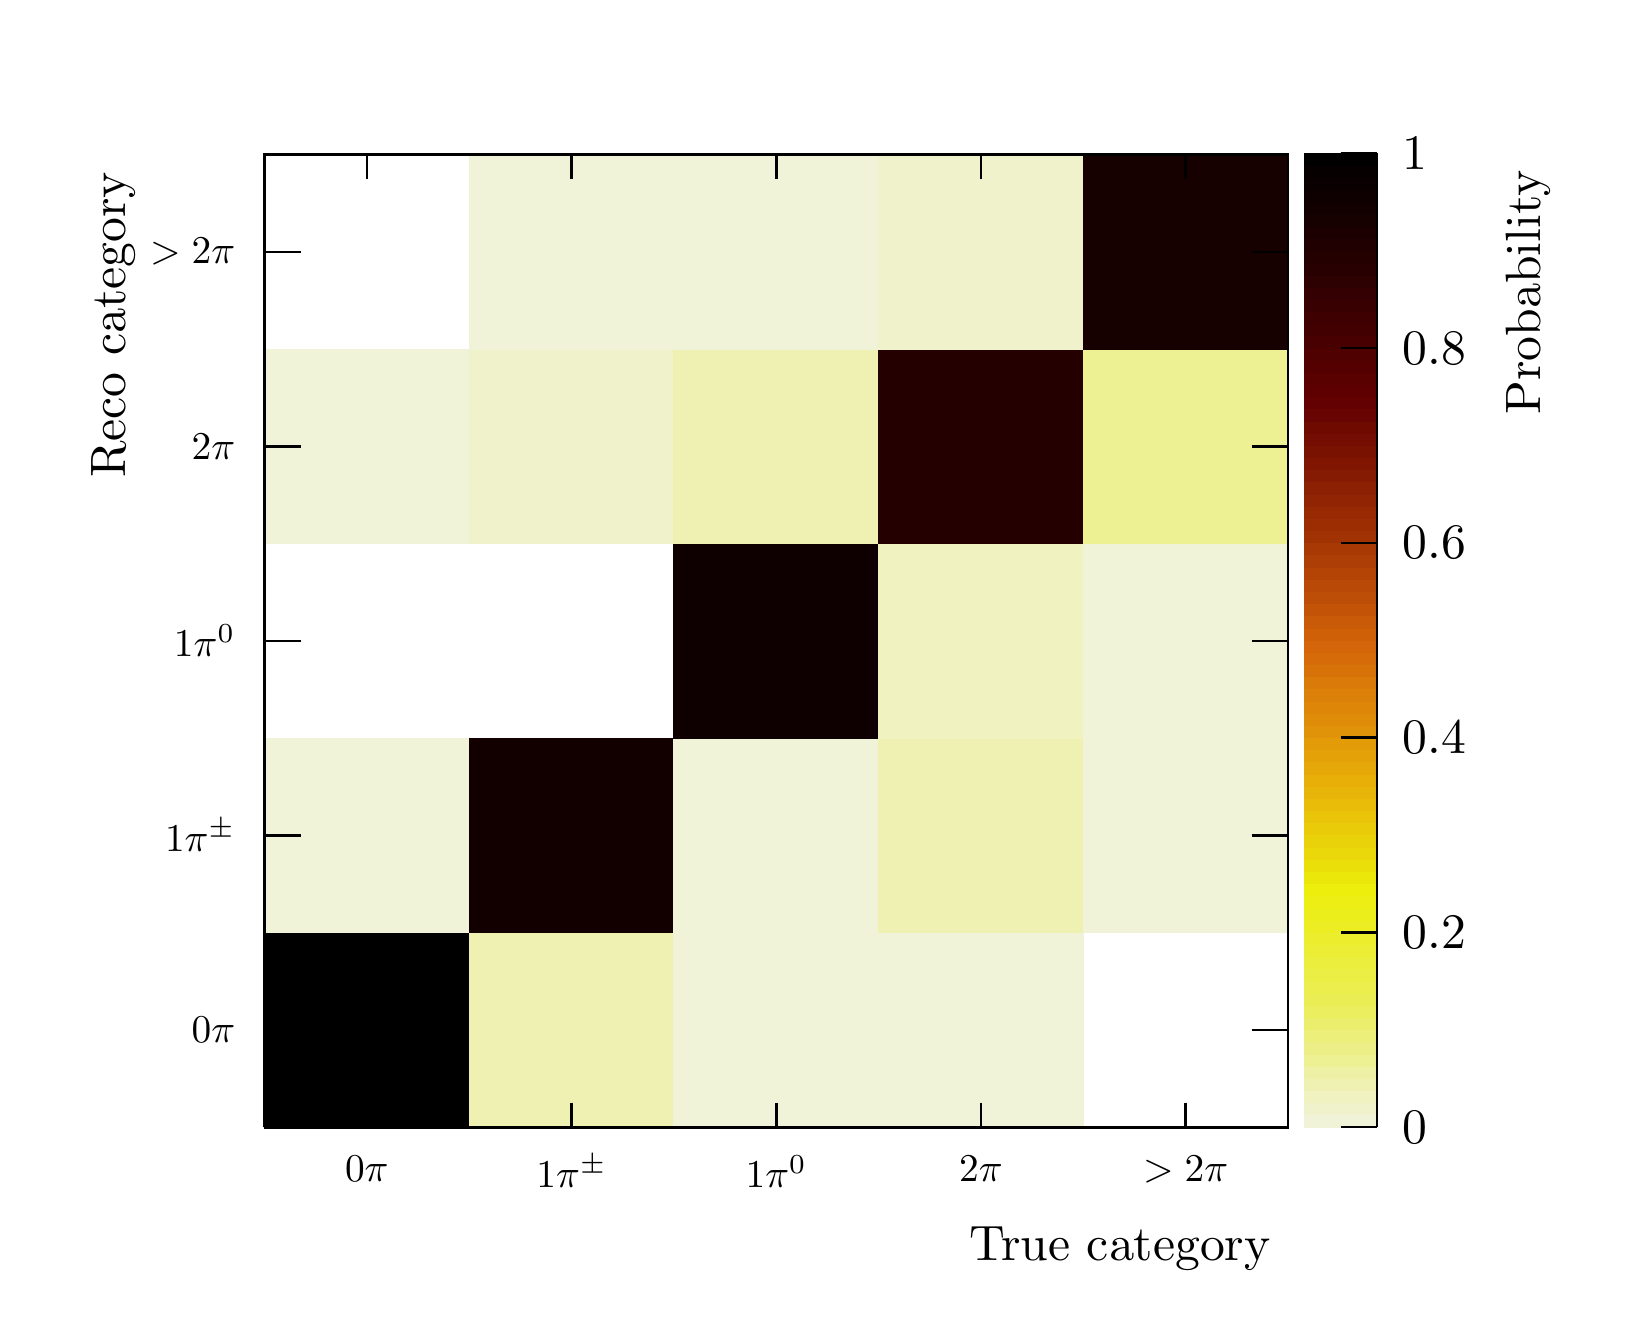
\begin{tikzpicture}
\pgfdeclareplotmark{cross} {
\pgfpathmoveto{\pgfpoint{-0.3\pgfplotmarksize}{\pgfplotmarksize}}
\pgfpathlineto{\pgfpoint{+0.3\pgfplotmarksize}{\pgfplotmarksize}}
\pgfpathlineto{\pgfpoint{+0.3\pgfplotmarksize}{0.3\pgfplotmarksize}}
\pgfpathlineto{\pgfpoint{+1\pgfplotmarksize}{0.3\pgfplotmarksize}}
\pgfpathlineto{\pgfpoint{+1\pgfplotmarksize}{-0.3\pgfplotmarksize}}
\pgfpathlineto{\pgfpoint{+0.3\pgfplotmarksize}{-0.3\pgfplotmarksize}}
\pgfpathlineto{\pgfpoint{+0.3\pgfplotmarksize}{-1.\pgfplotmarksize}}
\pgfpathlineto{\pgfpoint{-0.3\pgfplotmarksize}{-1.\pgfplotmarksize}}
\pgfpathlineto{\pgfpoint{-0.3\pgfplotmarksize}{-0.3\pgfplotmarksize}}
\pgfpathlineto{\pgfpoint{-1.\pgfplotmarksize}{-0.3\pgfplotmarksize}}
\pgfpathlineto{\pgfpoint{-1.\pgfplotmarksize}{0.3\pgfplotmarksize}}
\pgfpathlineto{\pgfpoint{-0.3\pgfplotmarksize}{0.3\pgfplotmarksize}}
\pgfpathclose
\pgfusepathqstroke
}
\pgfdeclareplotmark{cross*} {
\pgfpathmoveto{\pgfpoint{-0.3\pgfplotmarksize}{\pgfplotmarksize}}
\pgfpathlineto{\pgfpoint{+0.3\pgfplotmarksize}{\pgfplotmarksize}}
\pgfpathlineto{\pgfpoint{+0.3\pgfplotmarksize}{0.3\pgfplotmarksize}}
\pgfpathlineto{\pgfpoint{+1\pgfplotmarksize}{0.3\pgfplotmarksize}}
\pgfpathlineto{\pgfpoint{+1\pgfplotmarksize}{-0.3\pgfplotmarksize}}
\pgfpathlineto{\pgfpoint{+0.3\pgfplotmarksize}{-0.3\pgfplotmarksize}}
\pgfpathlineto{\pgfpoint{+0.3\pgfplotmarksize}{-1.\pgfplotmarksize}}
\pgfpathlineto{\pgfpoint{-0.3\pgfplotmarksize}{-1.\pgfplotmarksize}}
\pgfpathlineto{\pgfpoint{-0.3\pgfplotmarksize}{-0.3\pgfplotmarksize}}
\pgfpathlineto{\pgfpoint{-1.\pgfplotmarksize}{-0.3\pgfplotmarksize}}
\pgfpathlineto{\pgfpoint{-1.\pgfplotmarksize}{0.3\pgfplotmarksize}}
\pgfpathlineto{\pgfpoint{-0.3\pgfplotmarksize}{0.3\pgfplotmarksize}}
\pgfpathclose
\pgfusepathqfillstroke
}
\pgfdeclareplotmark{newstar} {
\pgfpathmoveto{\pgfqpoint{0pt}{\pgfplotmarksize}}
\pgfpathlineto{\pgfqpointpolar{44}{0.5\pgfplotmarksize}}
\pgfpathlineto{\pgfqpointpolar{18}{\pgfplotmarksize}}
\pgfpathlineto{\pgfqpointpolar{-20}{0.5\pgfplotmarksize}}
\pgfpathlineto{\pgfqpointpolar{-54}{\pgfplotmarksize}}
\pgfpathlineto{\pgfqpointpolar{-90}{0.5\pgfplotmarksize}}
\pgfpathlineto{\pgfqpointpolar{234}{\pgfplotmarksize}}
\pgfpathlineto{\pgfqpointpolar{198}{0.5\pgfplotmarksize}}
\pgfpathlineto{\pgfqpointpolar{162}{\pgfplotmarksize}}
\pgfpathlineto{\pgfqpointpolar{134}{0.5\pgfplotmarksize}}
\pgfpathclose
\pgfusepathqstroke
}
\pgfdeclareplotmark{newstar*} {
\pgfpathmoveto{\pgfqpoint{0pt}{\pgfplotmarksize}}
\pgfpathlineto{\pgfqpointpolar{44}{0.5\pgfplotmarksize}}
\pgfpathlineto{\pgfqpointpolar{18}{\pgfplotmarksize}}
\pgfpathlineto{\pgfqpointpolar{-20}{0.5\pgfplotmarksize}}
\pgfpathlineto{\pgfqpointpolar{-54}{\pgfplotmarksize}}
\pgfpathlineto{\pgfqpointpolar{-90}{0.5\pgfplotmarksize}}
\pgfpathlineto{\pgfqpointpolar{234}{\pgfplotmarksize}}
\pgfpathlineto{\pgfqpointpolar{198}{0.5\pgfplotmarksize}}
\pgfpathlineto{\pgfqpointpolar{162}{\pgfplotmarksize}}
\pgfpathlineto{\pgfqpointpolar{134}{0.5\pgfplotmarksize}}
\pgfpathclose
\pgfusepathqfillstroke
}
\definecolor{c}{rgb}{1,1,1};
\draw [color=c, fill=c] (0,0) rectangle (20,16.0446);
\draw [color=c, fill=c] (3,2.08579) rectangle (16,14.4401);
\definecolor{c}{rgb}{0,0,0};
\draw [c,line width=0.9] (3,2.08579) -- (3,14.4401) -- (16,14.4401) -- (16,2.08579) -- (3,2.08579);
\definecolor{c}{rgb}{1,1,1};
\draw [color=c, fill=c] (3,2.08579) rectangle (16,14.4401);
\definecolor{c}{rgb}{0,0,0};
\draw [c,line width=0.9] (3,2.08579) -- (3,14.4401) -- (16,14.4401) -- (16,2.08579) -- (3,2.08579);
\definecolor{c}{rgb}{0.00551471,0,0.000122549};
\draw [color=c, fill=c] (3,2.08579) rectangle (5.6,4.55666);
\definecolor{c}{rgb}{0.936875,0.945351,0.697027};
\draw [color=c, fill=c] (5.6,2.08579) rectangle (8.2,4.55666);
\definecolor{c}{rgb}{0.945984,0.951044,0.850727};
\draw [color=c, fill=c] (8.2,2.08579) rectangle (10.8,4.55666);
\draw [color=c, fill=c] (10.8,2.08579) rectangle (13.4,4.55666);
\draw [color=c, fill=c] (3,4.55666) rectangle (5.6,7.02752);
\definecolor{c}{rgb}{0.0716912,0,0.00159314};
\draw [color=c, fill=c] (5.6,4.55666) rectangle (8.2,7.02752);
\definecolor{c}{rgb}{0.945984,0.951044,0.850727};
\draw [color=c, fill=c] (8.2,4.55666) rectangle (10.8,7.02752);
\definecolor{c}{rgb}{0.936875,0.945351,0.697027};
\draw [color=c, fill=c] (10.8,4.55666) rectangle (13.4,7.02752);
\definecolor{c}{rgb}{0.945984,0.951044,0.850727};
\draw [color=c, fill=c] (13.4,4.55666) rectangle (16,7.02752);
\definecolor{c}{rgb}{0.0551471,0,0.00122549};
\draw [color=c, fill=c] (8.2,7.02752) rectangle (10.8,9.49838);
\definecolor{c}{rgb}{0.939911,0.947249,0.748261};
\draw [color=c, fill=c] (10.8,7.02752) rectangle (13.4,9.49838);
\definecolor{c}{rgb}{0.945984,0.951044,0.850727};
\draw [color=c, fill=c] (13.4,7.02752) rectangle (16,9.49838);
\draw [color=c, fill=c] (3,9.49838) rectangle (5.6,11.9692);
\definecolor{c}{rgb}{0.942948,0.949146,0.799494};
\draw [color=c, fill=c] (5.6,9.49838) rectangle (8.2,11.9692);
\definecolor{c}{rgb}{0.936875,0.945351,0.697027};
\draw [color=c, fill=c] (8.2,9.49838) rectangle (10.8,11.9692);
\definecolor{c}{rgb}{0.143382,0,0.00318627};
\draw [color=c, fill=c] (10.8,9.49838) rectangle (13.4,11.9692);
\definecolor{c}{rgb}{0.929791,0.940923,0.577483};
\draw [color=c, fill=c] (13.4,9.49838) rectangle (16,11.9692);
\definecolor{c}{rgb}{0.945984,0.951044,0.850727};
\draw [color=c, fill=c] (5.6,11.9692) rectangle (8.2,14.4401);
\draw [color=c, fill=c] (8.2,11.9692) rectangle (10.8,14.4401);
\definecolor{c}{rgb}{0.942948,0.949146,0.799494};
\draw [color=c, fill=c] (10.8,11.9692) rectangle (13.4,14.4401);
\definecolor{c}{rgb}{0.0882353,0,0.00196078};
\draw [color=c, fill=c] (13.4,11.9692) rectangle (16,14.4401);
\definecolor{c}{rgb}{0,0,0};
\draw [c,line width=0.9] (3,2.08579) -- (16,2.08579);
\draw [anchor=north] (4.3,1.90048) node[scale=1.42291, color=c, rotate=0]{$0\pi$};
\draw [anchor=north] (6.9,1.90048) node[scale=1.42291, color=c, rotate=0]{$1\pi^{\pm}$};
\draw [anchor=north] (9.5,1.90048) node[scale=1.42291, color=c, rotate=0]{$1\pi^{0}$};
\draw [anchor=north] (12.1,1.90048) node[scale=1.42291, color=c, rotate=0]{$2\pi$};
\draw [anchor=north] (14.7,1.90048) node[scale=1.42291, color=c, rotate=0]{$>2\pi$};
\draw [c,line width=0.9] (4.3,2.39866) -- (4.3,2.08579);
\draw [c,line width=0.9] (6.9,2.39866) -- (6.9,2.08579);
\draw [c,line width=0.9] (9.5,2.39866) -- (9.5,2.08579);
\draw [c,line width=0.9] (12.1,2.39866) -- (12.1,2.08579);
\draw [c,line width=0.9] (14.7,2.39866) -- (14.7,2.08579);
\draw [c,line width=0.9] (4.3,2.39866) -- (4.3,2.08579);
\draw [c,line width=0.9] (14.7,2.39866) -- (14.7,2.08579);
\draw [anchor= east] (16,0.545515) node[scale=1.7941, color=c, rotate=0]{ True category};
\draw [c,line width=0.9] (3,14.4401) -- (16,14.4401);
\draw [c,line width=0.9] (4.3,14.1272) -- (4.3,14.4401);
\draw [c,line width=0.9] (6.9,14.1272) -- (6.9,14.4401);
\draw [c,line width=0.9] (9.5,14.1272) -- (9.5,14.4401);
\draw [c,line width=0.9] (12.1,14.1272) -- (12.1,14.4401);
\draw [c,line width=0.9] (14.7,14.1272) -- (14.7,14.4401);
\draw [c,line width=0.9] (4.3,14.1272) -- (4.3,14.4401);
\draw [c,line width=0.9] (14.7,14.1272) -- (14.7,14.4401);
\draw [c,line width=0.9] (3,2.08579) -- (3,14.4401);
\draw [anchor= east] (2.805,3.32123) node[scale=1.42291, color=c, rotate=0]{$0\pi$};
\draw [anchor= east] (2.805,5.79209) node[scale=1.42291, color=c, rotate=0]{$1\pi^{\pm}$};
\draw [anchor= east] (2.805,8.26295) node[scale=1.42291, color=c, rotate=0]{$1\pi^{0}$};
\draw [anchor= east] (2.805,10.7338) node[scale=1.42291, color=c, rotate=0]{$2\pi$};
\draw [anchor= east] (2.805,13.2047) node[scale=1.42291, color=c, rotate=0]{$>2\pi$};
\draw [c,line width=0.9] (3.462,3.32123) -- (3,3.32123);
\draw [c,line width=0.9] (3.462,5.79209) -- (3,5.79209);
\draw [c,line width=0.9] (3.462,8.26295) -- (3,8.26295);
\draw [c,line width=0.9] (3.462,10.7338) -- (3,10.7338);
\draw [c,line width=0.9] (3.462,13.2047) -- (3,13.2047);
\draw [c,line width=0.9] (3.462,3.32123) -- (3,3.32123);
\draw [c,line width=0.9] (3.462,13.2047) -- (3,13.2047);
\draw [anchor= east] (1.08,14.4401) node[scale=1.7941, color=c, rotate=90]{ Reco category};
\draw [c,line width=0.9] (16,2.08579) -- (16,14.4401);
\draw [c,line width=0.9] (15.538,3.32123) -- (16,3.32123);
\draw [c,line width=0.9] (15.538,5.79209) -- (16,5.79209);
\draw [c,line width=0.9] (15.538,8.26295) -- (16,8.26295);
\draw [c,line width=0.9] (15.538,10.7338) -- (16,10.7338);
\draw [c,line width=0.9] (15.538,13.2047) -- (16,13.2047);
\draw [c,line width=0.9] (15.538,3.32123) -- (16,3.32123);
\draw [c,line width=0.9] (15.538,13.2047) -- (16,13.2047);
\definecolor{c}{rgb}{0.945984,0.951044,0.850727};
\draw [color=c, fill=c] (16.2117,2.08914) rectangle (17.1309,2.24373);
\definecolor{c}{rgb}{0.942948,0.949146,0.799494};
\draw [color=c, fill=c] (16.2117,2.24373) rectangle (17.1309,2.39833);
\definecolor{c}{rgb}{0.939911,0.947249,0.748261};
\draw [color=c, fill=c] (16.2117,2.39833) rectangle (17.1309,2.55292);
\definecolor{c}{rgb}{0.936875,0.945351,0.697027};
\draw [color=c, fill=c] (16.2117,2.55292) rectangle (17.1309,2.70752);
\definecolor{c}{rgb}{0.933839,0.943453,0.645794};
\draw [color=c, fill=c] (16.2117,2.70752) rectangle (17.1309,2.86212);
\definecolor{c}{rgb}{0.929791,0.940923,0.577483};
\draw [color=c, fill=c] (16.2117,2.86212) rectangle (17.1309,3.01671);
\definecolor{c}{rgb}{0.926755,0.939026,0.526249};
\draw [color=c, fill=c] (16.2117,3.01671) rectangle (17.1309,3.17131);
\definecolor{c}{rgb}{0.923719,0.937128,0.475016};
\draw [color=c, fill=c] (16.2117,3.17131) rectangle (17.1309,3.32591);
\definecolor{c}{rgb}{0.920683,0.935231,0.423782};
\draw [color=c, fill=c] (16.2117,3.32591) rectangle (17.1309,3.4805);
\definecolor{c}{rgb}{0.917647,0.933333,0.372549};
\draw [color=c, fill=c] (16.2117,3.4805) rectangle (17.1309,3.6351);
\definecolor{c}{rgb}{0.919118,0.933333,0.331373};
\draw [color=c, fill=c] (16.2117,3.6351) rectangle (17.1309,3.78969);
\definecolor{c}{rgb}{0.920221,0.933333,0.30049};
\draw [color=c, fill=c] (16.2117,3.78969) rectangle (17.1309,3.94429);
\definecolor{c}{rgb}{0.921324,0.933333,0.269608};
\draw [color=c, fill=c] (16.2117,3.94429) rectangle (17.1309,4.09889);
\definecolor{c}{rgb}{0.922426,0.933333,0.238725};
\draw [color=c, fill=c] (16.2117,4.09889) rectangle (17.1309,4.25348);
\definecolor{c}{rgb}{0.923529,0.933333,0.207843};
\draw [color=c, fill=c] (16.2117,4.25348) rectangle (17.1309,4.40808);
\definecolor{c}{rgb}{0.924632,0.933333,0.176961};
\draw [color=c, fill=c] (16.2117,4.40808) rectangle (17.1309,4.56267);
\definecolor{c}{rgb}{0.926103,0.933333,0.135784};
\draw [color=c, fill=c] (16.2117,4.56267) rectangle (17.1309,4.71727);
\definecolor{c}{rgb}{0.927206,0.933333,0.104902};
\draw [color=c, fill=c] (16.2117,4.71727) rectangle (17.1309,4.87187);
\definecolor{c}{rgb}{0.928309,0.933333,0.0740196};
\draw [color=c, fill=c] (16.2117,4.87187) rectangle (17.1309,5.02646);
\definecolor{c}{rgb}{0.929412,0.933333,0.0431373};
\draw [color=c, fill=c] (16.2117,5.02646) rectangle (17.1309,5.18106);
\definecolor{c}{rgb}{0.926838,0.907598,0.0420343};
\draw [color=c, fill=c] (16.2117,5.18106) rectangle (17.1309,5.33565);
\definecolor{c}{rgb}{0.923407,0.873284,0.0405637};
\draw [color=c, fill=c] (16.2117,5.33565) rectangle (17.1309,5.49025);
\definecolor{c}{rgb}{0.920833,0.847549,0.0394608};
\draw [color=c, fill=c] (16.2117,5.49025) rectangle (17.1309,5.64485);
\definecolor{c}{rgb}{0.91826,0.821814,0.0383578};
\draw [color=c, fill=c] (16.2117,5.64485) rectangle (17.1309,5.79944);
\definecolor{c}{rgb}{0.915686,0.796078,0.0372549};
\draw [color=c, fill=c] (16.2117,5.79944) rectangle (17.1309,5.95404);
\definecolor{c}{rgb}{0.913113,0.770343,0.036152};
\draw [color=c, fill=c] (16.2117,5.95404) rectangle (17.1309,6.10864);
\definecolor{c}{rgb}{0.909681,0.736029,0.0346814};
\draw [color=c, fill=c] (16.2117,6.10864) rectangle (17.1309,6.26323);
\definecolor{c}{rgb}{0.907108,0.710294,0.0335784};
\draw [color=c, fill=c] (16.2117,6.26323) rectangle (17.1309,6.41783);
\definecolor{c}{rgb}{0.904534,0.684559,0.0324755};
\draw [color=c, fill=c] (16.2117,6.41783) rectangle (17.1309,6.57242);
\definecolor{c}{rgb}{0.901961,0.658824,0.0313726};
\draw [color=c, fill=c] (16.2117,6.57242) rectangle (17.1309,6.72702);
\definecolor{c}{rgb}{0.895343,0.634191,0.0317402};
\draw [color=c, fill=c] (16.2117,6.72702) rectangle (17.1309,6.88162);
\definecolor{c}{rgb}{0.888726,0.609559,0.0321078};
\draw [color=c, fill=c] (16.2117,6.88162) rectangle (17.1309,7.03621);
\definecolor{c}{rgb}{0.879902,0.576716,0.032598};
\draw [color=c, fill=c] (16.2117,7.03621) rectangle (17.1309,7.19081);
\definecolor{c}{rgb}{0.873284,0.552083,0.0329657};
\draw [color=c, fill=c] (16.2117,7.19081) rectangle (17.1309,7.3454);
\definecolor{c}{rgb}{0.866667,0.527451,0.0333333};
\draw [color=c, fill=c] (16.2117,7.3454) rectangle (17.1309,7.5);
\definecolor{c}{rgb}{0.860049,0.502819,0.033701};
\draw [color=c, fill=c] (16.2117,7.5) rectangle (17.1309,7.6546);
\definecolor{c}{rgb}{0.853431,0.478186,0.0340686};
\draw [color=c, fill=c] (16.2117,7.6546) rectangle (17.1309,7.80919);
\definecolor{c}{rgb}{0.844608,0.445343,0.0345588};
\draw [color=c, fill=c] (16.2117,7.80919) rectangle (17.1309,7.96379);
\definecolor{c}{rgb}{0.83799,0.420711,0.0349265};
\draw [color=c, fill=c] (16.2117,7.96379) rectangle (17.1309,8.11838);
\definecolor{c}{rgb}{0.831373,0.396078,0.0352941};
\draw [color=c, fill=c] (16.2117,8.11838) rectangle (17.1309,8.27298);
\definecolor{c}{rgb}{0.810784,0.37549,0.0330882};
\draw [color=c, fill=c] (16.2117,8.27298) rectangle (17.1309,8.42758);
\definecolor{c}{rgb}{0.790196,0.354902,0.0308824};
\draw [color=c, fill=c] (16.2117,8.42758) rectangle (17.1309,8.58217);
\definecolor{c}{rgb}{0.762745,0.327451,0.0279412};
\draw [color=c, fill=c] (16.2117,8.58217) rectangle (17.1309,8.73677);
\definecolor{c}{rgb}{0.742157,0.306863,0.0257353};
\draw [color=c, fill=c] (16.2117,8.73677) rectangle (17.1309,8.89137);
\definecolor{c}{rgb}{0.721569,0.286275,0.0235294};
\draw [color=c, fill=c] (16.2117,8.89137) rectangle (17.1309,9.04596);
\definecolor{c}{rgb}{0.70098,0.265686,0.0213235};
\draw [color=c, fill=c] (16.2117,9.04596) rectangle (17.1309,9.20056);
\definecolor{c}{rgb}{0.680392,0.245098,0.0191176};
\draw [color=c, fill=c] (16.2117,9.20056) rectangle (17.1309,9.35515);
\definecolor{c}{rgb}{0.659804,0.22451,0.0169118};
\draw [color=c, fill=c] (16.2117,9.35515) rectangle (17.1309,9.50975);
\definecolor{c}{rgb}{0.632353,0.197059,0.0139706};
\draw [color=c, fill=c] (16.2117,9.50975) rectangle (17.1309,9.66435);
\definecolor{c}{rgb}{0.611765,0.176471,0.0117647};
\draw [color=c, fill=c] (16.2117,9.66435) rectangle (17.1309,9.81894);
\definecolor{c}{rgb}{0.590809,0.159926,0.0110294};
\draw [color=c, fill=c] (16.2117,9.81894) rectangle (17.1309,9.97354);
\definecolor{c}{rgb}{0.569853,0.143382,0.0102941};
\draw [color=c, fill=c] (16.2117,9.97354) rectangle (17.1309,10.1281);
\definecolor{c}{rgb}{0.548897,0.126838,0.00955882};
\draw [color=c, fill=c] (16.2117,10.1281) rectangle (17.1309,10.2827);
\definecolor{c}{rgb}{0.520956,0.104779,0.00857843};
\draw [color=c, fill=c] (16.2117,10.2827) rectangle (17.1309,10.4373);
\definecolor{c}{rgb}{0.5,0.0882353,0.00784314};
\draw [color=c, fill=c] (16.2117,10.4373) rectangle (17.1309,10.5919);
\definecolor{c}{rgb}{0.479044,0.0716912,0.00710784};
\draw [color=c, fill=c] (16.2117,10.5919) rectangle (17.1309,10.7465);
\definecolor{c}{rgb}{0.458088,0.0551471,0.00637255};
\draw [color=c, fill=c] (16.2117,10.7465) rectangle (17.1309,10.9011);
\definecolor{c}{rgb}{0.437132,0.0386029,0.00563726};
\draw [color=c, fill=c] (16.2117,10.9011) rectangle (17.1309,11.0557);
\definecolor{c}{rgb}{0.409191,0.0165441,0.00465686};
\draw [color=c, fill=c] (16.2117,11.0557) rectangle (17.1309,11.2103);
\definecolor{c}{rgb}{0.388235,0,0.00392157};
\draw [color=c, fill=c] (16.2117,11.2103) rectangle (17.1309,11.3649);
\definecolor{c}{rgb}{0.368382,0,0.00392157};
\draw [color=c, fill=c] (16.2117,11.3649) rectangle (17.1309,11.5195);
\definecolor{c}{rgb}{0.348529,0,0.00392157};
\draw [color=c, fill=c] (16.2117,11.5195) rectangle (17.1309,11.6741);
\definecolor{c}{rgb}{0.328676,0,0.00392157};
\draw [color=c, fill=c] (16.2117,11.6741) rectangle (17.1309,11.8287);
\definecolor{c}{rgb}{0.308824,0,0.00392157};
\draw [color=c, fill=c] (16.2117,11.8287) rectangle (17.1309,11.9833);
\definecolor{c}{rgb}{0.282353,0,0.00392157};
\draw [color=c, fill=c] (16.2117,11.9833) rectangle (17.1309,12.1379);
\definecolor{c}{rgb}{0.2625,0,0.00392157};
\draw [color=c, fill=c] (16.2117,12.1379) rectangle (17.1309,12.2925);
\definecolor{c}{rgb}{0.242647,0,0.00392157};
\draw [color=c, fill=c] (16.2117,12.2925) rectangle (17.1309,12.4471);
\definecolor{c}{rgb}{0.222794,0,0.00392157};
\draw [color=c, fill=c] (16.2117,12.4471) rectangle (17.1309,12.6017);
\definecolor{c}{rgb}{0.202941,0,0.00392157};
\draw [color=c, fill=c] (16.2117,12.6017) rectangle (17.1309,12.7563);
\definecolor{c}{rgb}{0.176471,0,0.00392157};
\draw [color=c, fill=c] (16.2117,12.7563) rectangle (17.1309,12.9109);
\definecolor{c}{rgb}{0.159926,0,0.00355392};
\draw [color=c, fill=c] (16.2117,12.9109) rectangle (17.1309,13.0655);
\definecolor{c}{rgb}{0.143382,0,0.00318627};
\draw [color=c, fill=c] (16.2117,13.0655) rectangle (17.1309,13.2201);
\definecolor{c}{rgb}{0.126838,0,0.00281863};
\draw [color=c, fill=c] (16.2117,13.2201) rectangle (17.1309,13.3747);
\definecolor{c}{rgb}{0.110294,0,0.00245098};
\draw [color=c, fill=c] (16.2117,13.3747) rectangle (17.1309,13.5292);
\definecolor{c}{rgb}{0.0882353,0,0.00196078};
\draw [color=c, fill=c] (16.2117,13.5292) rectangle (17.1309,13.6838);
\definecolor{c}{rgb}{0.0716912,0,0.00159314};
\draw [color=c, fill=c] (16.2117,13.6838) rectangle (17.1309,13.8384);
\definecolor{c}{rgb}{0.0551471,0,0.00122549};
\draw [color=c, fill=c] (16.2117,13.8384) rectangle (17.1309,13.993);
\definecolor{c}{rgb}{0.0386029,0,0.000857843};
\draw [color=c, fill=c] (16.2117,13.993) rectangle (17.1309,14.1476);
\definecolor{c}{rgb}{0.0220588,0,0.000490196};
\draw [color=c, fill=c] (16.2117,14.1476) rectangle (17.1309,14.3022);
\definecolor{c}{rgb}{0.00551471,0,0.000122549};
\draw [color=c, fill=c] (16.2117,14.3022) rectangle (17.1309,14.4568);
\definecolor{c}{rgb}{0,0,0};
\draw [c,line width=0.9] (17.1309,2.08914) -- (17.1309,14.4568);
\draw [c,line width=0.9] (16.6684,2.08914) -- (17.1309,2.08914);
\draw [c,line width=0.9] (16.6684,4.56267) -- (17.1309,4.56267);
\draw [c,line width=0.9] (16.6684,7.03621) -- (17.1309,7.03621);
\draw [c,line width=0.9] (16.6684,9.50975) -- (17.1309,9.50975);
\draw [c,line width=0.9] (16.6684,11.9833) -- (17.1309,11.9833);
\draw [c,line width=0.9] (16.6684,14.4568) -- (17.1309,14.4568);
\draw [c,line width=0.9] (16.6684,14.4568) -- (17.1309,14.4568);
\draw [anchor= west] (17.2309,2.08914) node[scale=1.7941, color=c, rotate=0]{0};
\draw [anchor= west] (17.2309,4.56267) node[scale=1.7941, color=c, rotate=0]{0.2};
\draw [anchor= west] (17.2309,7.03621) node[scale=1.7941, color=c, rotate=0]{0.4};
\draw [anchor= west] (17.2309,9.50975) node[scale=1.7941, color=c, rotate=0]{0.6};
\draw [anchor= west] (17.2309,11.9833) node[scale=1.7941, color=c, rotate=0]{0.8};
\draw [anchor= west] (17.2309,14.4568) node[scale=1.7941, color=c, rotate=0]{1};
\draw [anchor= east] (19.0509,14.4568) node[scale=1.7941, color=c, rotate=90]{ Probability};
\definecolor{c}{rgb}{1,1,1};
\draw [color=c, fill=c] (2,15.0819) rectangle (18,15.9643);
\definecolor{c}{rgb}{0,0,0};
%\draw (10,15.5231) node[scale=1.67037, color=c, rotate=0]{Final state confusion matrix in HPgTPC};
\end{tikzpicture}

		\end{adjustbox}
	\end{minipage}
	\hfill
	\begin{minipage}[t]{.5\linewidth}
		\begin{adjustbox}{max totalsize=\linewidth, center}
			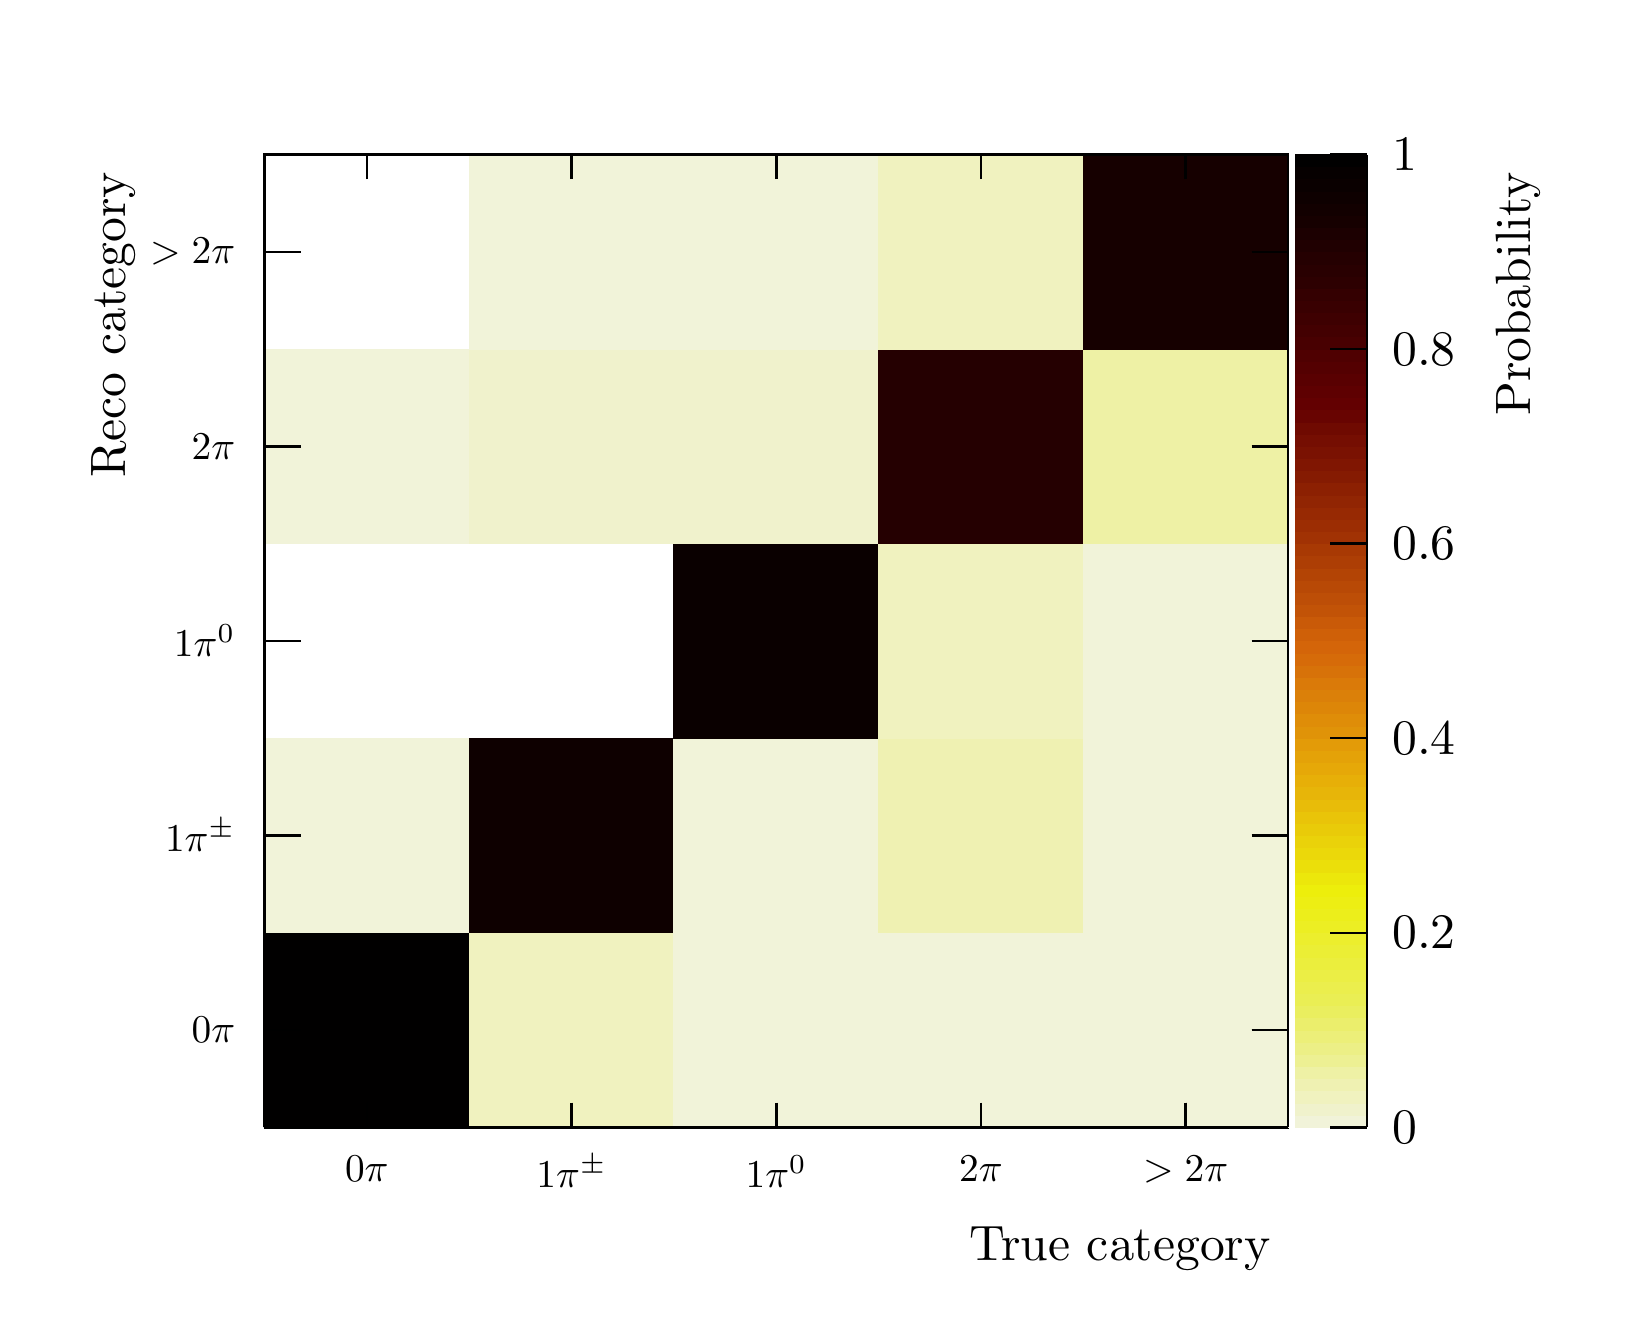
\begin{tikzpicture}
\pgfdeclareplotmark{cross} {
\pgfpathmoveto{\pgfpoint{-0.3\pgfplotmarksize}{\pgfplotmarksize}}
\pgfpathlineto{\pgfpoint{+0.3\pgfplotmarksize}{\pgfplotmarksize}}
\pgfpathlineto{\pgfpoint{+0.3\pgfplotmarksize}{0.3\pgfplotmarksize}}
\pgfpathlineto{\pgfpoint{+1\pgfplotmarksize}{0.3\pgfplotmarksize}}
\pgfpathlineto{\pgfpoint{+1\pgfplotmarksize}{-0.3\pgfplotmarksize}}
\pgfpathlineto{\pgfpoint{+0.3\pgfplotmarksize}{-0.3\pgfplotmarksize}}
\pgfpathlineto{\pgfpoint{+0.3\pgfplotmarksize}{-1.\pgfplotmarksize}}
\pgfpathlineto{\pgfpoint{-0.3\pgfplotmarksize}{-1.\pgfplotmarksize}}
\pgfpathlineto{\pgfpoint{-0.3\pgfplotmarksize}{-0.3\pgfplotmarksize}}
\pgfpathlineto{\pgfpoint{-1.\pgfplotmarksize}{-0.3\pgfplotmarksize}}
\pgfpathlineto{\pgfpoint{-1.\pgfplotmarksize}{0.3\pgfplotmarksize}}
\pgfpathlineto{\pgfpoint{-0.3\pgfplotmarksize}{0.3\pgfplotmarksize}}
\pgfpathclose
\pgfusepathqstroke
}
\pgfdeclareplotmark{cross*} {
\pgfpathmoveto{\pgfpoint{-0.3\pgfplotmarksize}{\pgfplotmarksize}}
\pgfpathlineto{\pgfpoint{+0.3\pgfplotmarksize}{\pgfplotmarksize}}
\pgfpathlineto{\pgfpoint{+0.3\pgfplotmarksize}{0.3\pgfplotmarksize}}
\pgfpathlineto{\pgfpoint{+1\pgfplotmarksize}{0.3\pgfplotmarksize}}
\pgfpathlineto{\pgfpoint{+1\pgfplotmarksize}{-0.3\pgfplotmarksize}}
\pgfpathlineto{\pgfpoint{+0.3\pgfplotmarksize}{-0.3\pgfplotmarksize}}
\pgfpathlineto{\pgfpoint{+0.3\pgfplotmarksize}{-1.\pgfplotmarksize}}
\pgfpathlineto{\pgfpoint{-0.3\pgfplotmarksize}{-1.\pgfplotmarksize}}
\pgfpathlineto{\pgfpoint{-0.3\pgfplotmarksize}{-0.3\pgfplotmarksize}}
\pgfpathlineto{\pgfpoint{-1.\pgfplotmarksize}{-0.3\pgfplotmarksize}}
\pgfpathlineto{\pgfpoint{-1.\pgfplotmarksize}{0.3\pgfplotmarksize}}
\pgfpathlineto{\pgfpoint{-0.3\pgfplotmarksize}{0.3\pgfplotmarksize}}
\pgfpathclose
\pgfusepathqfillstroke
}
\pgfdeclareplotmark{newstar} {
\pgfpathmoveto{\pgfqpoint{0pt}{\pgfplotmarksize}}
\pgfpathlineto{\pgfqpointpolar{44}{0.5\pgfplotmarksize}}
\pgfpathlineto{\pgfqpointpolar{18}{\pgfplotmarksize}}
\pgfpathlineto{\pgfqpointpolar{-20}{0.5\pgfplotmarksize}}
\pgfpathlineto{\pgfqpointpolar{-54}{\pgfplotmarksize}}
\pgfpathlineto{\pgfqpointpolar{-90}{0.5\pgfplotmarksize}}
\pgfpathlineto{\pgfqpointpolar{234}{\pgfplotmarksize}}
\pgfpathlineto{\pgfqpointpolar{198}{0.5\pgfplotmarksize}}
\pgfpathlineto{\pgfqpointpolar{162}{\pgfplotmarksize}}
\pgfpathlineto{\pgfqpointpolar{134}{0.5\pgfplotmarksize}}
\pgfpathclose
\pgfusepathqstroke
}
\pgfdeclareplotmark{newstar*} {
\pgfpathmoveto{\pgfqpoint{0pt}{\pgfplotmarksize}}
\pgfpathlineto{\pgfqpointpolar{44}{0.5\pgfplotmarksize}}
\pgfpathlineto{\pgfqpointpolar{18}{\pgfplotmarksize}}
\pgfpathlineto{\pgfqpointpolar{-20}{0.5\pgfplotmarksize}}
\pgfpathlineto{\pgfqpointpolar{-54}{\pgfplotmarksize}}
\pgfpathlineto{\pgfqpointpolar{-90}{0.5\pgfplotmarksize}}
\pgfpathlineto{\pgfqpointpolar{234}{\pgfplotmarksize}}
\pgfpathlineto{\pgfqpointpolar{198}{0.5\pgfplotmarksize}}
\pgfpathlineto{\pgfqpointpolar{162}{\pgfplotmarksize}}
\pgfpathlineto{\pgfqpointpolar{134}{0.5\pgfplotmarksize}}
\pgfpathclose
\pgfusepathqfillstroke
}
\definecolor{c}{rgb}{1,1,1};
\draw [color=c, fill=c] (0,0) rectangle (20,16.0446);
\draw [color=c, fill=c] (3,2.08579) rectangle (16,14.4401);
\definecolor{c}{rgb}{0,0,0};
\draw [c,line width=0.9] (3,2.08579) -- (3,14.4401) -- (16,14.4401) -- (16,2.08579) -- (3,2.08579);
\definecolor{c}{rgb}{1,1,1};
\draw [color=c, fill=c] (3,2.08579) rectangle (16,14.4401);
\definecolor{c}{rgb}{0,0,0};
\draw [c,line width=0.9] (3,2.08579) -- (3,14.4401) -- (16,14.4401) -- (16,2.08579) -- (3,2.08579);
\definecolor{c}{rgb}{0.00551471,0,0.000122549};
\draw [color=c, fill=c] (3,2.08579) rectangle (5.6,4.55666);
\definecolor{c}{rgb}{0.939911,0.947249,0.748261};
\draw [color=c, fill=c] (5.6,2.08579) rectangle (8.2,4.55666);
\definecolor{c}{rgb}{0.945984,0.951044,0.850727};
\draw [color=c, fill=c] (8.2,2.08579) rectangle (10.8,4.55666);
\draw [color=c, fill=c] (10.8,2.08579) rectangle (13.4,4.55666);
\draw [color=c, fill=c] (13.4,2.08579) rectangle (16,4.55666);
\draw [color=c, fill=c] (3,4.55666) rectangle (5.6,7.02752);
\definecolor{c}{rgb}{0.0551471,0,0.00122549};
\draw [color=c, fill=c] (5.6,4.55666) rectangle (8.2,7.02752);
\definecolor{c}{rgb}{0.945984,0.951044,0.850727};
\draw [color=c, fill=c] (8.2,4.55666) rectangle (10.8,7.02752);
\definecolor{c}{rgb}{0.936875,0.945351,0.697027};
\draw [color=c, fill=c] (10.8,4.55666) rectangle (13.4,7.02752);
\definecolor{c}{rgb}{0.945984,0.951044,0.850727};
\draw [color=c, fill=c] (13.4,4.55666) rectangle (16,7.02752);
\definecolor{c}{rgb}{0.0386029,0,0.000857843};
\draw [color=c, fill=c] (8.2,7.02752) rectangle (10.8,9.49838);
\definecolor{c}{rgb}{0.939911,0.947249,0.748261};
\draw [color=c, fill=c] (10.8,7.02752) rectangle (13.4,9.49838);
\definecolor{c}{rgb}{0.945984,0.951044,0.850727};
\draw [color=c, fill=c] (13.4,7.02752) rectangle (16,9.49838);
\draw [color=c, fill=c] (3,9.49838) rectangle (5.6,11.9692);
\definecolor{c}{rgb}{0.942948,0.949146,0.799494};
\draw [color=c, fill=c] (5.6,9.49838) rectangle (8.2,11.9692);
\draw [color=c, fill=c] (8.2,9.49838) rectangle (10.8,11.9692);
\definecolor{c}{rgb}{0.143382,0,0.00318627};
\draw [color=c, fill=c] (10.8,9.49838) rectangle (13.4,11.9692);
\definecolor{c}{rgb}{0.933839,0.943453,0.645794};
\draw [color=c, fill=c] (13.4,9.49838) rectangle (16,11.9692);
\definecolor{c}{rgb}{0.945984,0.951044,0.850727};
\draw [color=c, fill=c] (5.6,11.9692) rectangle (8.2,14.4401);
\draw [color=c, fill=c] (8.2,11.9692) rectangle (10.8,14.4401);
\definecolor{c}{rgb}{0.939911,0.947249,0.748261};
\draw [color=c, fill=c] (10.8,11.9692) rectangle (13.4,14.4401);
\definecolor{c}{rgb}{0.0882353,0,0.00196078};
\draw [color=c, fill=c] (13.4,11.9692) rectangle (16,14.4401);
\definecolor{c}{rgb}{0,0,0};
\draw [c,line width=0.9] (3,2.08579) -- (16,2.08579);
\draw [anchor=north] (4.3,1.90048) node[scale=1.42291, color=c, rotate=0]{$0\pi$};
\draw [anchor=north] (6.9,1.90048) node[scale=1.42291, color=c, rotate=0]{$1\pi^{\pm}$};
\draw [anchor=north] (9.5,1.90048) node[scale=1.42291, color=c, rotate=0]{$1\pi^{0}$};
\draw [anchor=north] (12.1,1.90048) node[scale=1.42291, color=c, rotate=0]{$2\pi$};
\draw [anchor=north] (14.7,1.90048) node[scale=1.42291, color=c, rotate=0]{$>2\pi$};
\draw [c,line width=0.9] (4.3,2.39866) -- (4.3,2.08579);
\draw [c,line width=0.9] (6.9,2.39866) -- (6.9,2.08579);
\draw [c,line width=0.9] (9.5,2.39866) -- (9.5,2.08579);
\draw [c,line width=0.9] (12.1,2.39866) -- (12.1,2.08579);
\draw [c,line width=0.9] (14.7,2.39866) -- (14.7,2.08579);
\draw [c,line width=0.9] (4.3,2.39866) -- (4.3,2.08579);
\draw [c,line width=0.9] (14.7,2.39866) -- (14.7,2.08579);
\draw [anchor= east] (16,0.545515) node[scale=1.7941, color=c, rotate=0]{ True category};
\draw [c,line width=0.9] (3,14.4401) -- (16,14.4401);
\draw [c,line width=0.9] (4.3,14.1272) -- (4.3,14.4401);
\draw [c,line width=0.9] (6.9,14.1272) -- (6.9,14.4401);
\draw [c,line width=0.9] (9.5,14.1272) -- (9.5,14.4401);
\draw [c,line width=0.9] (12.1,14.1272) -- (12.1,14.4401);
\draw [c,line width=0.9] (14.7,14.1272) -- (14.7,14.4401);
\draw [c,line width=0.9] (4.3,14.1272) -- (4.3,14.4401);
\draw [c,line width=0.9] (14.7,14.1272) -- (14.7,14.4401);
\draw [c,line width=0.9] (3,2.08579) -- (3,14.4401);
\draw [anchor= east] (2.805,3.32123) node[scale=1.42291, color=c, rotate=0]{$0\pi$};
\draw [anchor= east] (2.805,5.79209) node[scale=1.42291, color=c, rotate=0]{$1\pi^{\pm}$};
\draw [anchor= east] (2.805,8.26295) node[scale=1.42291, color=c, rotate=0]{$1\pi^{0}$};
\draw [anchor= east] (2.805,10.7338) node[scale=1.42291, color=c, rotate=0]{$2\pi$};
\draw [anchor= east] (2.805,13.2047) node[scale=1.42291, color=c, rotate=0]{$>2\pi$};
\draw [c,line width=0.9] (3.462,3.32123) -- (3,3.32123);
\draw [c,line width=0.9] (3.462,5.79209) -- (3,5.79209);
\draw [c,line width=0.9] (3.462,8.26295) -- (3,8.26295);
\draw [c,line width=0.9] (3.462,10.7338) -- (3,10.7338);
\draw [c,line width=0.9] (3.462,13.2047) -- (3,13.2047);
\draw [c,line width=0.9] (3.462,3.32123) -- (3,3.32123);
\draw [c,line width=0.9] (3.462,13.2047) -- (3,13.2047);
\draw [anchor= east] (1.08,14.4401) node[scale=1.7941, color=c, rotate=90]{ Reco category};
\draw [c,line width=0.9] (16,2.08579) -- (16,14.4401);
\draw [c,line width=0.9] (15.538,3.32123) -- (16,3.32123);
\draw [c,line width=0.9] (15.538,5.79209) -- (16,5.79209);
\draw [c,line width=0.9] (15.538,8.26295) -- (16,8.26295);
\draw [c,line width=0.9] (15.538,10.7338) -- (16,10.7338);
\draw [c,line width=0.9] (15.538,13.2047) -- (16,13.2047);
\draw [c,line width=0.9] (15.538,3.32123) -- (16,3.32123);
\draw [c,line width=0.9] (15.538,13.2047) -- (16,13.2047);
\definecolor{c}{rgb}{0.945984,0.951044,0.850727};
\draw [color=c, fill=c] (16.1,2.08579) rectangle (17,2.24022);
\definecolor{c}{rgb}{0.942948,0.949146,0.799494};
\draw [color=c, fill=c] (16.1,2.24022) rectangle (17,2.39465);
\definecolor{c}{rgb}{0.939911,0.947249,0.748261};
\draw [color=c, fill=c] (16.1,2.39465) rectangle (17,2.54908);
\definecolor{c}{rgb}{0.936875,0.945351,0.697027};
\draw [color=c, fill=c] (16.1,2.54908) rectangle (17,2.70351);
\definecolor{c}{rgb}{0.933839,0.943453,0.645794};
\draw [color=c, fill=c] (16.1,2.70351) rectangle (17,2.85794);
\definecolor{c}{rgb}{0.929791,0.940923,0.577483};
\draw [color=c, fill=c] (16.1,2.85794) rectangle (17,3.01237);
\definecolor{c}{rgb}{0.926755,0.939026,0.526249};
\draw [color=c, fill=c] (16.1,3.01237) rectangle (17,3.1668);
\definecolor{c}{rgb}{0.923719,0.937128,0.475016};
\draw [color=c, fill=c] (16.1,3.1668) rectangle (17,3.32123);
\definecolor{c}{rgb}{0.920683,0.935231,0.423782};
\draw [color=c, fill=c] (16.1,3.32123) rectangle (17,3.47565);
\definecolor{c}{rgb}{0.917647,0.933333,0.372549};
\draw [color=c, fill=c] (16.1,3.47565) rectangle (17,3.63008);
\definecolor{c}{rgb}{0.919118,0.933333,0.331373};
\draw [color=c, fill=c] (16.1,3.63008) rectangle (17,3.78451);
\definecolor{c}{rgb}{0.920221,0.933333,0.30049};
\draw [color=c, fill=c] (16.1,3.78451) rectangle (17,3.93894);
\definecolor{c}{rgb}{0.921324,0.933333,0.269608};
\draw [color=c, fill=c] (16.1,3.93894) rectangle (17,4.09337);
\definecolor{c}{rgb}{0.922426,0.933333,0.238725};
\draw [color=c, fill=c] (16.1,4.09337) rectangle (17,4.2478);
\definecolor{c}{rgb}{0.923529,0.933333,0.207843};
\draw [color=c, fill=c] (16.1,4.2478) rectangle (17,4.40223);
\definecolor{c}{rgb}{0.924632,0.933333,0.176961};
\draw [color=c, fill=c] (16.1,4.40223) rectangle (17,4.55666);
\definecolor{c}{rgb}{0.926103,0.933333,0.135784};
\draw [color=c, fill=c] (16.1,4.55666) rectangle (17,4.71109);
\definecolor{c}{rgb}{0.927206,0.933333,0.104902};
\draw [color=c, fill=c] (16.1,4.71109) rectangle (17,4.86552);
\definecolor{c}{rgb}{0.928309,0.933333,0.0740196};
\draw [color=c, fill=c] (16.1,4.86552) rectangle (17,5.01994);
\definecolor{c}{rgb}{0.929412,0.933333,0.0431373};
\draw [color=c, fill=c] (16.1,5.01994) rectangle (17,5.17437);
\definecolor{c}{rgb}{0.926838,0.907598,0.0420343};
\draw [color=c, fill=c] (16.1,5.17437) rectangle (17,5.3288);
\definecolor{c}{rgb}{0.923407,0.873284,0.0405637};
\draw [color=c, fill=c] (16.1,5.3288) rectangle (17,5.48323);
\definecolor{c}{rgb}{0.920833,0.847549,0.0394608};
\draw [color=c, fill=c] (16.1,5.48323) rectangle (17,5.63766);
\definecolor{c}{rgb}{0.91826,0.821814,0.0383578};
\draw [color=c, fill=c] (16.1,5.63766) rectangle (17,5.79209);
\definecolor{c}{rgb}{0.915686,0.796078,0.0372549};
\draw [color=c, fill=c] (16.1,5.79209) rectangle (17,5.94652);
\definecolor{c}{rgb}{0.913113,0.770343,0.036152};
\draw [color=c, fill=c] (16.1,5.94652) rectangle (17,6.10095);
\definecolor{c}{rgb}{0.909681,0.736029,0.0346814};
\draw [color=c, fill=c] (16.1,6.10095) rectangle (17,6.25538);
\definecolor{c}{rgb}{0.907108,0.710294,0.0335784};
\draw [color=c, fill=c] (16.1,6.25538) rectangle (17,6.40981);
\definecolor{c}{rgb}{0.904534,0.684559,0.0324755};
\draw [color=c, fill=c] (16.1,6.40981) rectangle (17,6.56423);
\definecolor{c}{rgb}{0.901961,0.658824,0.0313726};
\draw [color=c, fill=c] (16.1,6.56423) rectangle (17,6.71866);
\definecolor{c}{rgb}{0.895343,0.634191,0.0317402};
\draw [color=c, fill=c] (16.1,6.71866) rectangle (17,6.87309);
\definecolor{c}{rgb}{0.888726,0.609559,0.0321078};
\draw [color=c, fill=c] (16.1,6.87309) rectangle (17,7.02752);
\definecolor{c}{rgb}{0.879902,0.576716,0.032598};
\draw [color=c, fill=c] (16.1,7.02752) rectangle (17,7.18195);
\definecolor{c}{rgb}{0.873284,0.552083,0.0329657};
\draw [color=c, fill=c] (16.1,7.18195) rectangle (17,7.33638);
\definecolor{c}{rgb}{0.866667,0.527451,0.0333333};
\draw [color=c, fill=c] (16.1,7.33638) rectangle (17,7.49081);
\definecolor{c}{rgb}{0.860049,0.502819,0.033701};
\draw [color=c, fill=c] (16.1,7.49081) rectangle (17,7.64524);
\definecolor{c}{rgb}{0.853431,0.478186,0.0340686};
\draw [color=c, fill=c] (16.1,7.64524) rectangle (17,7.79967);
\definecolor{c}{rgb}{0.844608,0.445343,0.0345588};
\draw [color=c, fill=c] (16.1,7.79967) rectangle (17,7.95409);
\definecolor{c}{rgb}{0.83799,0.420711,0.0349265};
\draw [color=c, fill=c] (16.1,7.95409) rectangle (17,8.10852);
\definecolor{c}{rgb}{0.831373,0.396078,0.0352941};
\draw [color=c, fill=c] (16.1,8.10852) rectangle (17,8.26295);
\definecolor{c}{rgb}{0.810784,0.37549,0.0330882};
\draw [color=c, fill=c] (16.1,8.26295) rectangle (17,8.41738);
\definecolor{c}{rgb}{0.790196,0.354902,0.0308824};
\draw [color=c, fill=c] (16.1,8.41738) rectangle (17,8.57181);
\definecolor{c}{rgb}{0.762745,0.327451,0.0279412};
\draw [color=c, fill=c] (16.1,8.57181) rectangle (17,8.72624);
\definecolor{c}{rgb}{0.742157,0.306863,0.0257353};
\draw [color=c, fill=c] (16.1,8.72624) rectangle (17,8.88067);
\definecolor{c}{rgb}{0.721569,0.286275,0.0235294};
\draw [color=c, fill=c] (16.1,8.88067) rectangle (17,9.0351);
\definecolor{c}{rgb}{0.70098,0.265686,0.0213235};
\draw [color=c, fill=c] (16.1,9.0351) rectangle (17,9.18953);
\definecolor{c}{rgb}{0.680392,0.245098,0.0191176};
\draw [color=c, fill=c] (16.1,9.18953) rectangle (17,9.34396);
\definecolor{c}{rgb}{0.659804,0.22451,0.0169118};
\draw [color=c, fill=c] (16.1,9.34396) rectangle (17,9.49838);
\definecolor{c}{rgb}{0.632353,0.197059,0.0139706};
\draw [color=c, fill=c] (16.1,9.49838) rectangle (17,9.65281);
\definecolor{c}{rgb}{0.611765,0.176471,0.0117647};
\draw [color=c, fill=c] (16.1,9.65281) rectangle (17,9.80724);
\definecolor{c}{rgb}{0.590809,0.159926,0.0110294};
\draw [color=c, fill=c] (16.1,9.80724) rectangle (17,9.96167);
\definecolor{c}{rgb}{0.569853,0.143382,0.0102941};
\draw [color=c, fill=c] (16.1,9.96167) rectangle (17,10.1161);
\definecolor{c}{rgb}{0.548897,0.126838,0.00955882};
\draw [color=c, fill=c] (16.1,10.1161) rectangle (17,10.2705);
\definecolor{c}{rgb}{0.520956,0.104779,0.00857843};
\draw [color=c, fill=c] (16.1,10.2705) rectangle (17,10.425);
\definecolor{c}{rgb}{0.5,0.0882353,0.00784314};
\draw [color=c, fill=c] (16.1,10.425) rectangle (17,10.5794);
\definecolor{c}{rgb}{0.479044,0.0716912,0.00710784};
\draw [color=c, fill=c] (16.1,10.5794) rectangle (17,10.7338);
\definecolor{c}{rgb}{0.458088,0.0551471,0.00637255};
\draw [color=c, fill=c] (16.1,10.7338) rectangle (17,10.8882);
\definecolor{c}{rgb}{0.437132,0.0386029,0.00563726};
\draw [color=c, fill=c] (16.1,10.8882) rectangle (17,11.0427);
\definecolor{c}{rgb}{0.409191,0.0165441,0.00465686};
\draw [color=c, fill=c] (16.1,11.0427) rectangle (17,11.1971);
\definecolor{c}{rgb}{0.388235,0,0.00392157};
\draw [color=c, fill=c] (16.1,11.1971) rectangle (17,11.3515);
\definecolor{c}{rgb}{0.368382,0,0.00392157};
\draw [color=c, fill=c] (16.1,11.3515) rectangle (17,11.506);
\definecolor{c}{rgb}{0.348529,0,0.00392157};
\draw [color=c, fill=c] (16.1,11.506) rectangle (17,11.6604);
\definecolor{c}{rgb}{0.328676,0,0.00392157};
\draw [color=c, fill=c] (16.1,11.6604) rectangle (17,11.8148);
\definecolor{c}{rgb}{0.308824,0,0.00392157};
\draw [color=c, fill=c] (16.1,11.8148) rectangle (17,11.9692);
\definecolor{c}{rgb}{0.282353,0,0.00392157};
\draw [color=c, fill=c] (16.1,11.9692) rectangle (17,12.1237);
\definecolor{c}{rgb}{0.2625,0,0.00392157};
\draw [color=c, fill=c] (16.1,12.1237) rectangle (17,12.2781);
\definecolor{c}{rgb}{0.242647,0,0.00392157};
\draw [color=c, fill=c] (16.1,12.2781) rectangle (17,12.4325);
\definecolor{c}{rgb}{0.222794,0,0.00392157};
\draw [color=c, fill=c] (16.1,12.4325) rectangle (17,12.587);
\definecolor{c}{rgb}{0.202941,0,0.00392157};
\draw [color=c, fill=c] (16.1,12.587) rectangle (17,12.7414);
\definecolor{c}{rgb}{0.176471,0,0.00392157};
\draw [color=c, fill=c] (16.1,12.7414) rectangle (17,12.8958);
\definecolor{c}{rgb}{0.159926,0,0.00355392};
\draw [color=c, fill=c] (16.1,12.8958) rectangle (17,13.0503);
\definecolor{c}{rgb}{0.143382,0,0.00318627};
\draw [color=c, fill=c] (16.1,13.0503) rectangle (17,13.2047);
\definecolor{c}{rgb}{0.126838,0,0.00281863};
\draw [color=c, fill=c] (16.1,13.2047) rectangle (17,13.3591);
\definecolor{c}{rgb}{0.110294,0,0.00245098};
\draw [color=c, fill=c] (16.1,13.3591) rectangle (17,13.5135);
\definecolor{c}{rgb}{0.0882353,0,0.00196078};
\draw [color=c, fill=c] (16.1,13.5135) rectangle (17,13.668);
\definecolor{c}{rgb}{0.0716912,0,0.00159314};
\draw [color=c, fill=c] (16.1,13.668) rectangle (17,13.8224);
\definecolor{c}{rgb}{0.0551471,0,0.00122549};
\draw [color=c, fill=c] (16.1,13.8224) rectangle (17,13.9768);
\definecolor{c}{rgb}{0.0386029,0,0.000857843};
\draw [color=c, fill=c] (16.1,13.9768) rectangle (17,14.1313);
\definecolor{c}{rgb}{0.0220588,0,0.000490196};
\draw [color=c, fill=c] (16.1,14.1313) rectangle (17,14.2857);
\definecolor{c}{rgb}{0.00551471,0,0.000122549};
\draw [color=c, fill=c] (16.1,14.2857) rectangle (17,14.4401);
\definecolor{c}{rgb}{0,0,0};
\draw [c,line width=0.9] (17,2.08579) -- (17,14.4401);
\draw [c,line width=0.9] (16.538,2.08579) -- (17,2.08579);
\draw [c,line width=0.9] (16.538,4.55666) -- (17,4.55666);
\draw [c,line width=0.9] (16.538,7.02752) -- (17,7.02752);
\draw [c,line width=0.9] (16.538,9.49838) -- (17,9.49838);
\draw [c,line width=0.9] (16.538,11.9692) -- (17,11.9692);
\draw [c,line width=0.9] (16.538,14.4401) -- (17,14.4401);
\draw [c,line width=0.9] (16.538,14.4401) -- (17,14.4401);
\draw [anchor= west] (17.1,2.08579) node[scale=1.7941, color=c, rotate=0]{0};
\draw [anchor= west] (17.1,4.55666) node[scale=1.7941, color=c, rotate=0]{0.2};
\draw [anchor= west] (17.1,7.02752) node[scale=1.7941, color=c, rotate=0]{0.4};
\draw [anchor= west] (17.1,9.49838) node[scale=1.7941, color=c, rotate=0]{0.6};
\draw [anchor= west] (17.1,11.9692) node[scale=1.7941, color=c, rotate=0]{0.8};
\draw [anchor= west] (17.1,14.4401) node[scale=1.7941, color=c, rotate=0]{1};
\draw [anchor= east] (18.92,14.4401) node[scale=1.7941, color=c, rotate=90]{ Probability};
\definecolor{c}{rgb}{1,1,1};
\draw [color=c, fill=c] (2,15.0819) rectangle (18,15.9643);
\definecolor{c}{rgb}{0,0,0};
%\draw (10,15.5231) node[scale=1.67037, color=c, rotate=0]{Final state confusion matrix in HPgTPC};
\end{tikzpicture}

		\end{adjustbox}
	\end{minipage}
	\caption[Confusion matrices for pion multiplicities in ND-GAr]{Left: Confusion matrix for pion multiplicities in ND-GAr with the neutrino beam in FHC mode. Right: Confusion matrix for pion multiplicities in ND-GAr with the neutrino beam in RHC mode.}
	\label{fig:confusMatPi}
\end{figure}

\begin{figure}[h]
	\begin{minipage}[t]{.5\linewidth}
		\begin{adjustbox}{max totalsize=\linewidth, center}
			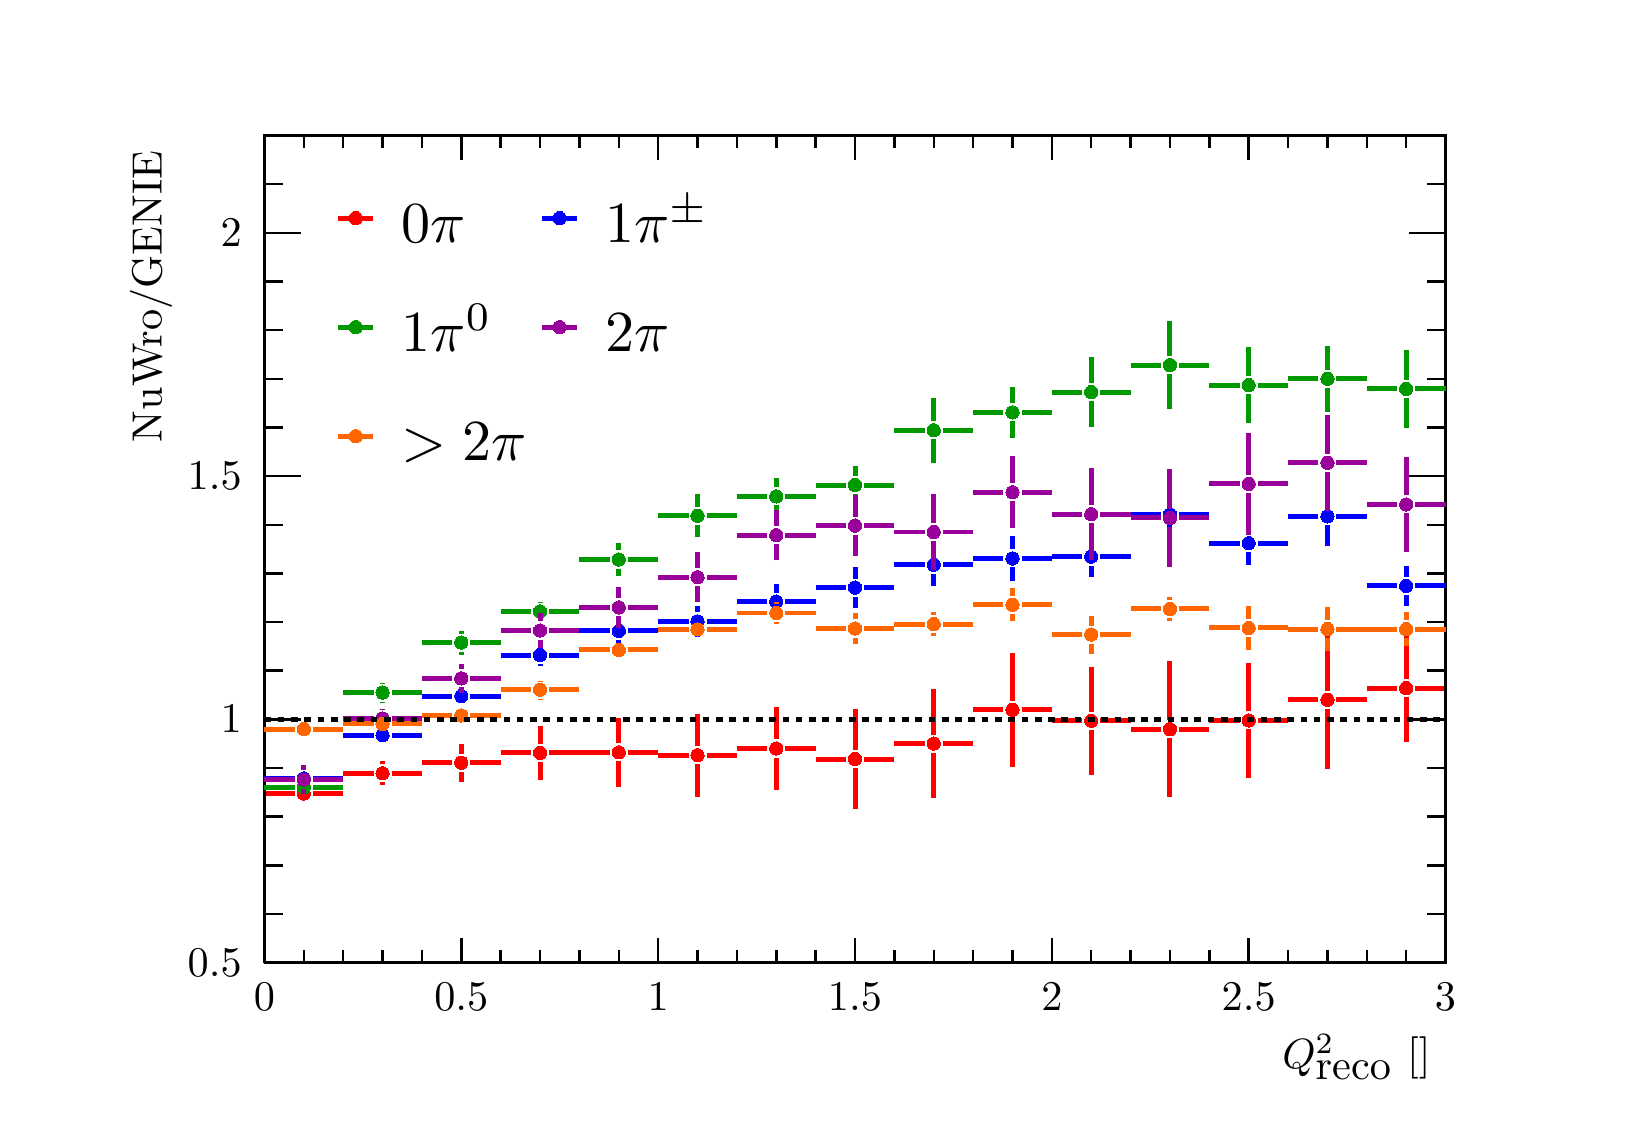
\begin{tikzpicture}
\pgfdeclareplotmark{cross} {
\pgfpathmoveto{\pgfpoint{-0.3\pgfplotmarksize}{\pgfplotmarksize}}
\pgfpathlineto{\pgfpoint{+0.3\pgfplotmarksize}{\pgfplotmarksize}}
\pgfpathlineto{\pgfpoint{+0.3\pgfplotmarksize}{0.3\pgfplotmarksize}}
\pgfpathlineto{\pgfpoint{+1\pgfplotmarksize}{0.3\pgfplotmarksize}}
\pgfpathlineto{\pgfpoint{+1\pgfplotmarksize}{-0.3\pgfplotmarksize}}
\pgfpathlineto{\pgfpoint{+0.3\pgfplotmarksize}{-0.3\pgfplotmarksize}}
\pgfpathlineto{\pgfpoint{+0.3\pgfplotmarksize}{-1.\pgfplotmarksize}}
\pgfpathlineto{\pgfpoint{-0.3\pgfplotmarksize}{-1.\pgfplotmarksize}}
\pgfpathlineto{\pgfpoint{-0.3\pgfplotmarksize}{-0.3\pgfplotmarksize}}
\pgfpathlineto{\pgfpoint{-1.\pgfplotmarksize}{-0.3\pgfplotmarksize}}
\pgfpathlineto{\pgfpoint{-1.\pgfplotmarksize}{0.3\pgfplotmarksize}}
\pgfpathlineto{\pgfpoint{-0.3\pgfplotmarksize}{0.3\pgfplotmarksize}}
\pgfpathclose
\pgfusepathqstroke
}
\pgfdeclareplotmark{cross*} {
\pgfpathmoveto{\pgfpoint{-0.3\pgfplotmarksize}{\pgfplotmarksize}}
\pgfpathlineto{\pgfpoint{+0.3\pgfplotmarksize}{\pgfplotmarksize}}
\pgfpathlineto{\pgfpoint{+0.3\pgfplotmarksize}{0.3\pgfplotmarksize}}
\pgfpathlineto{\pgfpoint{+1\pgfplotmarksize}{0.3\pgfplotmarksize}}
\pgfpathlineto{\pgfpoint{+1\pgfplotmarksize}{-0.3\pgfplotmarksize}}
\pgfpathlineto{\pgfpoint{+0.3\pgfplotmarksize}{-0.3\pgfplotmarksize}}
\pgfpathlineto{\pgfpoint{+0.3\pgfplotmarksize}{-1.\pgfplotmarksize}}
\pgfpathlineto{\pgfpoint{-0.3\pgfplotmarksize}{-1.\pgfplotmarksize}}
\pgfpathlineto{\pgfpoint{-0.3\pgfplotmarksize}{-0.3\pgfplotmarksize}}
\pgfpathlineto{\pgfpoint{-1.\pgfplotmarksize}{-0.3\pgfplotmarksize}}
\pgfpathlineto{\pgfpoint{-1.\pgfplotmarksize}{0.3\pgfplotmarksize}}
\pgfpathlineto{\pgfpoint{-0.3\pgfplotmarksize}{0.3\pgfplotmarksize}}
\pgfpathclose
\pgfusepathqfillstroke
}
\pgfdeclareplotmark{newstar} {
\pgfpathmoveto{\pgfqpoint{0pt}{\pgfplotmarksize}}
\pgfpathlineto{\pgfqpointpolar{44}{0.5\pgfplotmarksize}}
\pgfpathlineto{\pgfqpointpolar{18}{\pgfplotmarksize}}
\pgfpathlineto{\pgfqpointpolar{-20}{0.5\pgfplotmarksize}}
\pgfpathlineto{\pgfqpointpolar{-54}{\pgfplotmarksize}}
\pgfpathlineto{\pgfqpointpolar{-90}{0.5\pgfplotmarksize}}
\pgfpathlineto{\pgfqpointpolar{234}{\pgfplotmarksize}}
\pgfpathlineto{\pgfqpointpolar{198}{0.5\pgfplotmarksize}}
\pgfpathlineto{\pgfqpointpolar{162}{\pgfplotmarksize}}
\pgfpathlineto{\pgfqpointpolar{134}{0.5\pgfplotmarksize}}
\pgfpathclose
\pgfusepathqstroke
}
\pgfdeclareplotmark{newstar*} {
\pgfpathmoveto{\pgfqpoint{0pt}{\pgfplotmarksize}}
\pgfpathlineto{\pgfqpointpolar{44}{0.5\pgfplotmarksize}}
\pgfpathlineto{\pgfqpointpolar{18}{\pgfplotmarksize}}
\pgfpathlineto{\pgfqpointpolar{-20}{0.5\pgfplotmarksize}}
\pgfpathlineto{\pgfqpointpolar{-54}{\pgfplotmarksize}}
\pgfpathlineto{\pgfqpointpolar{-90}{0.5\pgfplotmarksize}}
\pgfpathlineto{\pgfqpointpolar{234}{\pgfplotmarksize}}
\pgfpathlineto{\pgfqpointpolar{198}{0.5\pgfplotmarksize}}
\pgfpathlineto{\pgfqpointpolar{162}{\pgfplotmarksize}}
\pgfpathlineto{\pgfqpointpolar{134}{0.5\pgfplotmarksize}}
\pgfpathclose
\pgfusepathqfillstroke
}
\definecolor{c}{rgb}{1,1,1};
\draw [color=c, fill=c] (0,0) rectangle (20,13.639);
\draw [color=c, fill=c] (3,1.77307) rectangle (18,12.2751);
\definecolor{c}{rgb}{0,0,0};
\draw [c,line width=0.9] (3,1.77307) -- (3,12.2751) -- (18,12.2751) -- (18,1.77307) -- (3,1.77307);
\definecolor{c}{rgb}{1,1,1};
\draw [color=c, fill=c] (3,1.77307) rectangle (18,12.2751);
\definecolor{c}{rgb}{0,0,0};
\draw [c,line width=0.9] (3,1.77307) -- (3,12.2751) -- (18,12.2751) -- (18,1.77307) -- (3,1.77307);
\definecolor{c}{rgb}{1,0,0};
\draw [c,line width=1.8] (3,3.91911) -- (3.38539,3.91911);
\draw [c,line width=1.8] (3.61461,3.91911) -- (4,3.91911);
\foreach \P in {(3.5,3.91911)}{\draw[mark options={color=c,fill=c},mark size=2.402402pt, line width=0.000000pt, mark=*] plot coordinates {\P};}
\draw [c,line width=1.8] (4.5,4.02491) -- (4.5,4.06197);
\draw [c,line width=1.8] (4.5,4.2912) -- (4.5,4.32827);
\draw [c,line width=1.8] (4,4.17659) -- (4.38539,4.17659);
\draw [c,line width=1.8] (4.61461,4.17659) -- (5,4.17659);
\foreach \P in {(4.5,4.17659)}{\draw[mark options={color=c,fill=c},mark size=2.402402pt, line width=0.000000pt, mark=*] plot coordinates {\P};}
\draw [c,line width=1.8] (5.5,4.06967) -- (5.5,4.19653);
\draw [c,line width=1.8] (5.5,4.42576) -- (5.5,4.55262);
\draw [c,line width=1.8] (5,4.31115) -- (5.38539,4.31115);
\draw [c,line width=1.8] (5.61461,4.31115) -- (6,4.31115);
\foreach \P in {(5.5,4.31115)}{\draw[mark options={color=c,fill=c},mark size=2.402402pt, line width=0.000000pt, mark=*] plot coordinates {\P};}
\draw [c,line width=1.8] (6.5,4.09054) -- (6.5,4.32215);
\draw [c,line width=1.8] (6.5,4.55138) -- (6.5,4.78299);
\draw [c,line width=1.8] (6,4.43676) -- (6.38539,4.43676);
\draw [c,line width=1.8] (6.61461,4.43676) -- (7,4.43676);
\foreach \P in {(6.5,4.43676)}{\draw[mark options={color=c,fill=c},mark size=2.402402pt, line width=0.000000pt, mark=*] plot coordinates {\P};}
\draw [c,line width=1.8] (7.5,4.00439) -- (7.5,4.32806);
\draw [c,line width=1.8] (7.5,4.55729) -- (7.5,4.88095);
\draw [c,line width=1.8] (7,4.44267) -- (7.38539,4.44267);
\draw [c,line width=1.8] (7.61461,4.44267) -- (8,4.44267);
\foreach \P in {(7.5,4.44267)}{\draw[mark options={color=c,fill=c},mark size=2.402402pt, line width=0.000000pt, mark=*] plot coordinates {\P};}
\draw [c,line width=1.8] (8.5,3.88168) -- (8.5,4.2921);
\draw [c,line width=1.8] (8.5,4.52133) -- (8.5,4.93175);
\draw [c,line width=1.8] (8,4.40671) -- (8.38539,4.40671);
\draw [c,line width=1.8] (8.61461,4.40671) -- (9,4.40671);
\foreach \P in {(8.5,4.40671)}{\draw[mark options={color=c,fill=c},mark size=2.402402pt, line width=0.000000pt, mark=*] plot coordinates {\P};}
\draw [c,line width=1.8] (9.5,3.95924) -- (9.5,4.37703);
\draw [c,line width=1.8] (9.5,4.60626) -- (9.5,5.02405);
\draw [c,line width=1.8] (9,4.49165) -- (9.38539,4.49165);
\draw [c,line width=1.8] (9.61461,4.49165) -- (10,4.49165);
\foreach \P in {(9.5,4.49165)}{\draw[mark options={color=c,fill=c},mark size=2.402402pt, line width=0.000000pt, mark=*] plot coordinates {\P};}
\draw [c,line width=1.8] (10.5,3.72077) -- (10.5,4.24284);
\draw [c,line width=1.8] (10.5,4.47207) -- (10.5,4.99414);
\draw [c,line width=1.8] (10,4.35746) -- (10.3854,4.35746);
\draw [c,line width=1.8] (10.6146,4.35746) -- (11,4.35746);
\foreach \P in {(10.5,4.35746)}{\draw[mark options={color=c,fill=c},mark size=2.402402pt, line width=0.000000pt, mark=*] plot coordinates {\P};}
\draw [c,line width=1.8] (11.5,3.86667) -- (11.5,4.43937);
\draw [c,line width=1.8] (11.5,4.6686) -- (11.5,5.24131);
\draw [c,line width=1.8] (11,4.55399) -- (11.3854,4.55399);
\draw [c,line width=1.8] (11.6146,4.55399) -- (12,4.55399);
\foreach \P in {(11.5,4.55399)}{\draw[mark options={color=c,fill=c},mark size=2.402402pt, line width=0.000000pt, mark=*] plot coordinates {\P};}
\draw [c,line width=1.8] (12.5,4.26285) -- (12.5,4.86913);
\draw [c,line width=1.8] (12.5,5.09835) -- (12.5,5.70464);
\draw [c,line width=1.8] (12,4.98374) -- (12.3854,4.98374);
\draw [c,line width=1.8] (12.6146,4.98374) -- (13,4.98374);
\foreach \P in {(12.5,4.98374)}{\draw[mark options={color=c,fill=c},mark size=2.402402pt, line width=0.000000pt, mark=*] plot coordinates {\P};}
\draw [c,line width=1.8] (13.5,4.16025) -- (13.5,4.72872);
\draw [c,line width=1.8] (13.5,4.95794) -- (13.5,5.52641);
\draw [c,line width=1.8] (13,4.84333) -- (13.3854,4.84333);
\draw [c,line width=1.8] (13.6146,4.84333) -- (14,4.84333);
\foreach \P in {(13.5,4.84333)}{\draw[mark options={color=c,fill=c},mark size=2.402402pt, line width=0.000000pt, mark=*] plot coordinates {\P};}
\draw [c,line width=1.8] (14.5,3.87445) -- (14.5,4.62216);
\draw [c,line width=1.8] (14.5,4.85139) -- (14.5,5.59911);
\draw [c,line width=1.8] (14,4.73678) -- (14.3854,4.73678);
\draw [c,line width=1.8] (14.6146,4.73678) -- (15,4.73678);
\foreach \P in {(14.5,4.73678)}{\draw[mark options={color=c,fill=c},mark size=2.402402pt, line width=0.000000pt, mark=*] plot coordinates {\P};}
\draw [c,line width=1.8] (15.5,4.12242) -- (15.5,4.73293);
\draw [c,line width=1.8] (15.5,4.96216) -- (15.5,5.57267);
\draw [c,line width=1.8] (15,4.84755) -- (15.3854,4.84755);
\draw [c,line width=1.8] (15.6146,4.84755) -- (16,4.84755);
\foreach \P in {(15.5,4.84755)}{\draw[mark options={color=c,fill=c},mark size=2.402402pt, line width=0.000000pt, mark=*] plot coordinates {\P};}
\draw [c,line width=1.8] (16.5,4.23132) -- (16.5,4.99592);
\draw [c,line width=1.8] (16.5,5.22515) -- (16.5,5.98976);
\draw [c,line width=1.8] (16,5.11054) -- (16.3854,5.11054);
\draw [c,line width=1.8] (16.6146,5.11054) -- (17,5.11054);
\foreach \P in {(16.5,5.11054)}{\draw[mark options={color=c,fill=c},mark size=2.402402pt, line width=0.000000pt, mark=*] plot coordinates {\P};}
\draw [c,line width=1.8] (17.5,4.57864) -- (17.5,5.14441);
\draw [c,line width=1.8] (17.5,5.37364) -- (17.5,5.93942);
\draw [c,line width=1.8] (17,5.25903) -- (17.3854,5.25903);
\draw [c,line width=1.8] (17.6146,5.25903) -- (18,5.25903);
\foreach \P in {(17.5,5.25903)}{\draw[mark options={color=c,fill=c},mark size=2.402402pt, line width=0.000000pt, mark=*] plot coordinates {\P};}
\definecolor{c}{rgb}{0,0,0};
\draw [c,line width=0.9] (3,1.77307) -- (18,1.77307);
\draw [c,line width=0.9] (3,2.07994) -- (3,1.77307);
\draw [c,line width=0.9] (3.5,1.9265) -- (3.5,1.77307);
\draw [c,line width=0.9] (4,1.9265) -- (4,1.77307);
\draw [c,line width=0.9] (4.5,1.9265) -- (4.5,1.77307);
\draw [c,line width=0.9] (5,1.9265) -- (5,1.77307);
\draw [c,line width=0.9] (5.5,2.07994) -- (5.5,1.77307);
\draw [c,line width=0.9] (6,1.9265) -- (6,1.77307);
\draw [c,line width=0.9] (6.5,1.9265) -- (6.5,1.77307);
\draw [c,line width=0.9] (7,1.9265) -- (7,1.77307);
\draw [c,line width=0.9] (7.5,1.9265) -- (7.5,1.77307);
\draw [c,line width=0.9] (8,2.07994) -- (8,1.77307);
\draw [c,line width=0.9] (8.5,1.9265) -- (8.5,1.77307);
\draw [c,line width=0.9] (9,1.9265) -- (9,1.77307);
\draw [c,line width=0.9] (9.5,1.9265) -- (9.5,1.77307);
\draw [c,line width=0.9] (10,1.9265) -- (10,1.77307);
\draw [c,line width=0.9] (10.5,2.07994) -- (10.5,1.77307);
\draw [c,line width=0.9] (11,1.9265) -- (11,1.77307);
\draw [c,line width=0.9] (11.5,1.9265) -- (11.5,1.77307);
\draw [c,line width=0.9] (12,1.9265) -- (12,1.77307);
\draw [c,line width=0.9] (12.5,1.9265) -- (12.5,1.77307);
\draw [c,line width=0.9] (13,2.07994) -- (13,1.77307);
\draw [c,line width=0.9] (13.5,1.9265) -- (13.5,1.77307);
\draw [c,line width=0.9] (14,1.9265) -- (14,1.77307);
\draw [c,line width=0.9] (14.5,1.9265) -- (14.5,1.77307);
\draw [c,line width=0.9] (15,1.9265) -- (15,1.77307);
\draw [c,line width=0.9] (15.5,2.07994) -- (15.5,1.77307);
\draw [c,line width=0.9] (16,1.9265) -- (16,1.77307);
\draw [c,line width=0.9] (16.5,1.9265) -- (16.5,1.77307);
\draw [c,line width=0.9] (17,1.9265) -- (17,1.77307);
\draw [c,line width=0.9] (17.5,1.9265) -- (17.5,1.77307);
\draw [c,line width=0.9] (18,2.07994) -- (18,1.77307);
\draw [c,line width=0.9] (18,2.07994) -- (18,1.77307);
\draw [anchor=base] (3,1.15931) node[scale=1.52731, color=c, rotate=0]{0};
\draw [anchor=base] (5.5,1.15931) node[scale=1.52731, color=c, rotate=0]{0.5};
\draw [anchor=base] (8,1.15931) node[scale=1.52731, color=c, rotate=0]{1};
\draw [anchor=base] (10.5,1.15931) node[scale=1.52731, color=c, rotate=0]{1.5};
\draw [anchor=base] (13,1.15931) node[scale=1.52731, color=c, rotate=0]{2};
\draw [anchor=base] (15.5,1.15931) node[scale=1.52731, color=c, rotate=0]{2.5};
\draw [anchor=base] (18,1.15931) node[scale=1.52731, color=c, rotate=0]{3};
\draw [anchor= east] (18,0.572837) node[scale=1.52731, color=c, rotate=0]{$Q^{2}_{\textrm{reco}}$ [\si{\GeV\squared}] };
\draw [c,line width=0.9] (3,12.2751) -- (18,12.2751);
\draw [c,line width=0.9] (3,11.9682) -- (3,12.2751);
\draw [c,line width=0.9] (3.5,12.1216) -- (3.5,12.2751);
\draw [c,line width=0.9] (4,12.1216) -- (4,12.2751);
\draw [c,line width=0.9] (4.5,12.1216) -- (4.5,12.2751);
\draw [c,line width=0.9] (5,12.1216) -- (5,12.2751);
\draw [c,line width=0.9] (5.5,11.9682) -- (5.5,12.2751);
\draw [c,line width=0.9] (6,12.1216) -- (6,12.2751);
\draw [c,line width=0.9] (6.5,12.1216) -- (6.5,12.2751);
\draw [c,line width=0.9] (7,12.1216) -- (7,12.2751);
\draw [c,line width=0.9] (7.5,12.1216) -- (7.5,12.2751);
\draw [c,line width=0.9] (8,11.9682) -- (8,12.2751);
\draw [c,line width=0.9] (8.5,12.1216) -- (8.5,12.2751);
\draw [c,line width=0.9] (9,12.1216) -- (9,12.2751);
\draw [c,line width=0.9] (9.5,12.1216) -- (9.5,12.2751);
\draw [c,line width=0.9] (10,12.1216) -- (10,12.2751);
\draw [c,line width=0.9] (10.5,11.9682) -- (10.5,12.2751);
\draw [c,line width=0.9] (11,12.1216) -- (11,12.2751);
\draw [c,line width=0.9] (11.5,12.1216) -- (11.5,12.2751);
\draw [c,line width=0.9] (12,12.1216) -- (12,12.2751);
\draw [c,line width=0.9] (12.5,12.1216) -- (12.5,12.2751);
\draw [c,line width=0.9] (13,11.9682) -- (13,12.2751);
\draw [c,line width=0.9] (13.5,12.1216) -- (13.5,12.2751);
\draw [c,line width=0.9] (14,12.1216) -- (14,12.2751);
\draw [c,line width=0.9] (14.5,12.1216) -- (14.5,12.2751);
\draw [c,line width=0.9] (15,12.1216) -- (15,12.2751);
\draw [c,line width=0.9] (15.5,11.9682) -- (15.5,12.2751);
\draw [c,line width=0.9] (16,12.1216) -- (16,12.2751);
\draw [c,line width=0.9] (16.5,12.1216) -- (16.5,12.2751);
\draw [c,line width=0.9] (17,12.1216) -- (17,12.2751);
\draw [c,line width=0.9] (17.5,12.1216) -- (17.5,12.2751);
\draw [c,line width=0.9] (18,11.9682) -- (18,12.2751);
\draw [c,line width=0.9] (18,11.9682) -- (18,12.2751);
\draw [c,line width=0.9] (3,1.77307) -- (3,12.2751);
\draw [c,line width=0.9] (3.462,1.77307) -- (3,1.77307);
\draw [c,line width=0.9] (3.231,2.39083) -- (3,2.39083);
\draw [c,line width=0.9] (3.231,3.0086) -- (3,3.0086);
\draw [c,line width=0.9] (3.231,3.62636) -- (3,3.62636);
\draw [c,line width=0.9] (3.231,4.24413) -- (3,4.24413);
\draw [c,line width=0.9] (3.462,4.86189) -- (3,4.86189);
\draw [c,line width=0.9] (3.231,5.47966) -- (3,5.47966);
\draw [c,line width=0.9] (3.231,6.09742) -- (3,6.09742);
\draw [c,line width=0.9] (3.231,6.71519) -- (3,6.71519);
\draw [c,line width=0.9] (3.231,7.33295) -- (3,7.33295);
\draw [c,line width=0.9] (3.462,7.95072) -- (3,7.95072);
\draw [c,line width=0.9] (3.231,8.56848) -- (3,8.56848);
\draw [c,line width=0.9] (3.231,9.18625) -- (3,9.18625);
\draw [c,line width=0.9] (3.231,9.80401) -- (3,9.80401);
\draw [c,line width=0.9] (3.231,10.4218) -- (3,10.4218);
\draw [c,line width=0.9] (3.462,11.0395) -- (3,11.0395);
\draw [c,line width=0.9] (3.462,11.0395) -- (3,11.0395);
\draw [c,line width=0.9] (3.231,11.6573) -- (3,11.6573);
\draw [c,line width=0.9] (3.231,12.2751) -- (3,12.2751);
\draw [anchor= east] (2.9,1.77307) node[scale=1.52731, color=c, rotate=0]{0.5};
\draw [anchor= east] (2.9,4.86189) node[scale=1.52731, color=c, rotate=0]{1};
\draw [anchor= east] (2.9,7.95072) node[scale=1.52731, color=c, rotate=0]{1.5};
\draw [anchor= east] (2.9,11.0395) node[scale=1.52731, color=c, rotate=0]{2};
\draw [anchor= east] (1.56,12.2751) node[scale=1.52731, color=c, rotate=90]{ NuWro/GENIE};
\draw [c,line width=0.9] (18,1.77307) -- (18,12.2751);
\draw [c,line width=0.9] (17.538,1.77307) -- (18,1.77307);
\draw [c,line width=0.9] (17.769,2.39083) -- (18,2.39083);
\draw [c,line width=0.9] (17.769,3.0086) -- (18,3.0086);
\draw [c,line width=0.9] (17.769,3.62636) -- (18,3.62636);
\draw [c,line width=0.9] (17.769,4.24413) -- (18,4.24413);
\draw [c,line width=0.9] (17.538,4.86189) -- (18,4.86189);
\draw [c,line width=0.9] (17.769,5.47966) -- (18,5.47966);
\draw [c,line width=0.9] (17.769,6.09742) -- (18,6.09742);
\draw [c,line width=0.9] (17.769,6.71519) -- (18,6.71519);
\draw [c,line width=0.9] (17.769,7.33295) -- (18,7.33295);
\draw [c,line width=0.9] (17.538,7.95072) -- (18,7.95072);
\draw [c,line width=0.9] (17.769,8.56848) -- (18,8.56848);
\draw [c,line width=0.9] (17.769,9.18625) -- (18,9.18625);
\draw [c,line width=0.9] (17.769,9.80401) -- (18,9.80401);
\draw [c,line width=0.9] (17.769,10.4218) -- (18,10.4218);
\draw [c,line width=0.9] (17.538,11.0395) -- (18,11.0395);
\draw [c,line width=0.9] (17.538,11.0395) -- (18,11.0395);
\draw [c,line width=0.9] (17.769,11.6573) -- (18,11.6573);
\draw [c,line width=0.9] (17.769,12.2751) -- (18,12.2751);
\definecolor{c}{rgb}{0,0,1};
\draw [c,line width=1.8] (3,4.11165) -- (3.38539,4.11165);
\draw [c,line width=1.8] (3.61461,4.11165) -- (4,4.11165);
\foreach \P in {(3.5,4.11165)}{\draw[mark options={color=c,fill=c},mark size=2.402402pt, line width=0.000000pt, mark=*] plot coordinates {\P};}
\draw [c,line width=1.8] (4,4.66109) -- (4.38539,4.66109);
\draw [c,line width=1.8] (4.61461,4.66109) -- (5,4.66109);
\foreach \P in {(4.5,4.66109)}{\draw[mark options={color=c,fill=c},mark size=2.402402pt, line width=0.000000pt, mark=*] plot coordinates {\P};}
\draw [c,line width=1.8] (5,5.15734) -- (5.38539,5.15734);
\draw [c,line width=1.8] (5.61461,5.15734) -- (6,5.15734);
\foreach \P in {(5.5,5.15734)}{\draw[mark options={color=c,fill=c},mark size=2.402402pt, line width=0.000000pt, mark=*] plot coordinates {\P};}
\draw [c,line width=1.8] (6.5,5.53786) -- (6.5,5.5637);
\draw [c,line width=1.8] (6.5,5.79293) -- (6.5,5.81878);
\draw [c,line width=1.8] (6,5.67832) -- (6.38539,5.67832);
\draw [c,line width=1.8] (6.61461,5.67832) -- (7,5.67832);
\foreach \P in {(6.5,5.67832)}{\draw[mark options={color=c,fill=c},mark size=2.402402pt, line width=0.000000pt, mark=*] plot coordinates {\P};}
\draw [c,line width=1.8] (7.5,5.81405) -- (7.5,5.87022);
\draw [c,line width=1.8] (7.5,6.09945) -- (7.5,6.15562);
\draw [c,line width=1.8] (7,5.98483) -- (7.38539,5.98483);
\draw [c,line width=1.8] (7.61461,5.98483) -- (8,5.98483);
\foreach \P in {(7.5,5.98483)}{\draw[mark options={color=c,fill=c},mark size=2.402402pt, line width=0.000000pt, mark=*] plot coordinates {\P};}
\draw [c,line width=1.8] (8.5,5.90476) -- (8.5,5.99085);
\draw [c,line width=1.8] (8.5,6.22008) -- (8.5,6.30618);
\draw [c,line width=1.8] (8,6.10547) -- (8.38539,6.10547);
\draw [c,line width=1.8] (8.61461,6.10547) -- (9,6.10547);
\foreach \P in {(8.5,6.10547)}{\draw[mark options={color=c,fill=c},mark size=2.402402pt, line width=0.000000pt, mark=*] plot coordinates {\P};}
\draw [c,line width=1.8] (9.5,6.13423) -- (9.5,6.2426);
\draw [c,line width=1.8] (9.5,6.47183) -- (9.5,6.58021);
\draw [c,line width=1.8] (9,6.35722) -- (9.38539,6.35722);
\draw [c,line width=1.8] (9.61461,6.35722) -- (10,6.35722);
\foreach \P in {(9.5,6.35722)}{\draw[mark options={color=c,fill=c},mark size=2.402402pt, line width=0.000000pt, mark=*] plot coordinates {\P};}
\draw [c,line width=1.8] (10.5,6.27812) -- (10.5,6.42058);
\draw [c,line width=1.8] (10.5,6.64981) -- (10.5,6.79227);
\draw [c,line width=1.8] (10,6.53519) -- (10.3854,6.53519);
\draw [c,line width=1.8] (10.6146,6.53519) -- (11,6.53519);
\foreach \P in {(10.5,6.53519)}{\draw[mark options={color=c,fill=c},mark size=2.402402pt, line width=0.000000pt, mark=*] plot coordinates {\P};}
\draw [c,line width=1.8] (11.5,6.55622) -- (11.5,6.71101);
\draw [c,line width=1.8] (11.5,6.94024) -- (11.5,7.09502);
\draw [c,line width=1.8] (11,6.82562) -- (11.3854,6.82562);
\draw [c,line width=1.8] (11.6146,6.82562) -- (12,6.82562);
\foreach \P in {(11.5,6.82562)}{\draw[mark options={color=c,fill=c},mark size=2.402402pt, line width=0.000000pt, mark=*] plot coordinates {\P};}
\draw [c,line width=1.8] (12.5,6.62113) -- (12.5,6.79021);
\draw [c,line width=1.8] (12.5,7.01944) -- (12.5,7.18851);
\draw [c,line width=1.8] (12,6.90482) -- (12.3854,6.90482);
\draw [c,line width=1.8] (12.6146,6.90482) -- (13,6.90482);
\foreach \P in {(12.5,6.90482)}{\draw[mark options={color=c,fill=c},mark size=2.402402pt, line width=0.000000pt, mark=*] plot coordinates {\P};}
\draw [c,line width=1.8] (13.5,6.67157) -- (13.5,6.81355);
\draw [c,line width=1.8] (13.5,7.04278) -- (13.5,7.18476);
\draw [c,line width=1.8] (13,6.92817) -- (13.3854,6.92817);
\draw [c,line width=1.8] (13.6146,6.92817) -- (14,6.92817);
\foreach \P in {(13.5,6.92817)}{\draw[mark options={color=c,fill=c},mark size=2.402402pt, line width=0.000000pt, mark=*] plot coordinates {\P};}
\draw [c,line width=1.8] (14.5,7.0792) -- (14.5,7.34926);
\draw [c,line width=1.8] (14.5,7.57849) -- (14.5,7.84855);
\draw [c,line width=1.8] (14,7.46388) -- (14.3854,7.46388);
\draw [c,line width=1.8] (14.6146,7.46388) -- (15,7.46388);
\foreach \P in {(14.5,7.46388)}{\draw[mark options={color=c,fill=c},mark size=2.402402pt, line width=0.000000pt, mark=*] plot coordinates {\P};}
\draw [c,line width=1.8] (15.5,6.82626) -- (15.5,6.98466);
\draw [c,line width=1.8] (15.5,7.21389) -- (15.5,7.37229);
\draw [c,line width=1.8] (15,7.09927) -- (15.3854,7.09927);
\draw [c,line width=1.8] (15.6146,7.09927) -- (16,7.09927);
\foreach \P in {(15.5,7.09927)}{\draw[mark options={color=c,fill=c},mark size=2.402402pt, line width=0.000000pt, mark=*] plot coordinates {\P};}
\draw [c,line width=1.8] (16.5,7.06422) -- (16.5,7.32444);
\draw [c,line width=1.8] (16.5,7.55366) -- (16.5,7.81388);
\draw [c,line width=1.8] (16,7.43905) -- (16.3854,7.43905);
\draw [c,line width=1.8] (16.6146,7.43905) -- (17,7.43905);
\foreach \P in {(16.5,7.43905)}{\draw[mark options={color=c,fill=c},mark size=2.402402pt, line width=0.000000pt, mark=*] plot coordinates {\P};}
\draw [c,line width=1.8] (17.5,6.30612) -- (17.5,6.44302);
\draw [c,line width=1.8] (17.5,6.67224) -- (17.5,6.80914);
\draw [c,line width=1.8] (17,6.55763) -- (17.3854,6.55763);
\draw [c,line width=1.8] (17.6146,6.55763) -- (18,6.55763);
\foreach \P in {(17.5,6.55763)}{\draw[mark options={color=c,fill=c},mark size=2.402402pt, line width=0.000000pt, mark=*] plot coordinates {\P};}
\definecolor{c}{rgb}{0,0.6,0};
\draw [c,line width=1.8] (3,4.00063) -- (3.38539,4.00063);
\draw [c,line width=1.8] (3.61461,4.00063) -- (4,4.00063);
\foreach \P in {(3.5,4.00063)}{\draw[mark options={color=c,fill=c},mark size=2.402402pt, line width=0.000000pt, mark=*] plot coordinates {\P};}
\draw [c,line width=1.8] (4.5,5.08587) -- (4.5,5.08748);
\draw [c,line width=1.8] (4.5,5.31671) -- (4.5,5.31831);
\draw [c,line width=1.8] (4,5.20209) -- (4.38539,5.20209);
\draw [c,line width=1.8] (4.61461,5.20209) -- (5,5.20209);
\foreach \P in {(4.5,5.20209)}{\draw[mark options={color=c,fill=c},mark size=2.402402pt, line width=0.000000pt, mark=*] plot coordinates {\P};}
\draw [c,line width=1.8] (5.5,5.6837) -- (5.5,5.72221);
\draw [c,line width=1.8] (5.5,5.95144) -- (5.5,5.98995);
\draw [c,line width=1.8] (5,5.83682) -- (5.38539,5.83682);
\draw [c,line width=1.8] (5.61461,5.83682) -- (6,5.83682);
\foreach \P in {(5.5,5.83682)}{\draw[mark options={color=c,fill=c},mark size=2.402402pt, line width=0.000000pt, mark=*] plot coordinates {\P};}
\draw [c,line width=1.8] (6.5,6.11477) -- (6.5,6.11856);
\draw [c,line width=1.8] (6.5,6.34778) -- (6.5,6.35157);
\draw [c,line width=1.8] (6,6.23317) -- (6.38539,6.23317);
\draw [c,line width=1.8] (6.61461,6.23317) -- (7,6.23317);
\foreach \P in {(6.5,6.23317)}{\draw[mark options={color=c,fill=c},mark size=2.402402pt, line width=0.000000pt, mark=*] plot coordinates {\P};}
\draw [c,line width=1.8] (7.5,6.67663) -- (7.5,6.77696);
\draw [c,line width=1.8] (7.5,7.00619) -- (7.5,7.10653);
\draw [c,line width=1.8] (7,6.89158) -- (7.38539,6.89158);
\draw [c,line width=1.8] (7.61461,6.89158) -- (8,6.89158);
\foreach \P in {(7.5,6.89158)}{\draw[mark options={color=c,fill=c},mark size=2.402402pt, line width=0.000000pt, mark=*] plot coordinates {\P};}
\draw [c,line width=1.8] (8.5,7.17253) -- (8.5,7.33205);
\draw [c,line width=1.8] (8.5,7.56127) -- (8.5,7.72078);
\draw [c,line width=1.8] (8,7.44666) -- (8.38539,7.44666);
\draw [c,line width=1.8] (8.61461,7.44666) -- (9,7.44666);
\foreach \P in {(8.5,7.44666)}{\draw[mark options={color=c,fill=c},mark size=2.402402pt, line width=0.000000pt, mark=*] plot coordinates {\P};}
\draw [c,line width=1.8] (9.5,7.46544) -- (9.5,7.57908);
\draw [c,line width=1.8] (9.5,7.8083) -- (9.5,7.92194);
\draw [c,line width=1.8] (9,7.69369) -- (9.38539,7.69369);
\draw [c,line width=1.8] (9.61461,7.69369) -- (10,7.69369);
\foreach \P in {(9.5,7.69369)}{\draw[mark options={color=c,fill=c},mark size=2.402402pt, line width=0.000000pt, mark=*] plot coordinates {\P};}
\draw [c,line width=1.8] (10.5,7.5936) -- (10.5,7.72286);
\draw [c,line width=1.8] (10.5,7.95209) -- (10.5,8.08135);
\draw [c,line width=1.8] (10,7.83748) -- (10.3854,7.83748);
\draw [c,line width=1.8] (10.6146,7.83748) -- (11,7.83748);
\foreach \P in {(10.5,7.83748)}{\draw[mark options={color=c,fill=c},mark size=2.402402pt, line width=0.000000pt, mark=*] plot coordinates {\P};}
\draw [c,line width=1.8] (11.5,8.11736) -- (11.5,8.41826);
\draw [c,line width=1.8] (11.5,8.64749) -- (11.5,8.9484);
\draw [c,line width=1.8] (11,8.53288) -- (11.3854,8.53288);
\draw [c,line width=1.8] (11.6146,8.53288) -- (12,8.53288);
\foreach \P in {(11.5,8.53288)}{\draw[mark options={color=c,fill=c},mark size=2.402402pt, line width=0.000000pt, mark=*] plot coordinates {\P};}
\draw [c,line width=1.8] (12.5,8.43939) -- (12.5,8.64546);
\draw [c,line width=1.8] (12.5,8.87468) -- (12.5,9.08075);
\draw [c,line width=1.8] (12,8.76007) -- (12.3854,8.76007);
\draw [c,line width=1.8] (12.6146,8.76007) -- (13,8.76007);
\foreach \P in {(12.5,8.76007)}{\draw[mark options={color=c,fill=c},mark size=2.402402pt, line width=0.000000pt, mark=*] plot coordinates {\P};}
\draw [c,line width=1.8] (13.5,8.57217) -- (13.5,8.90391);
\draw [c,line width=1.8] (13.5,9.13314) -- (13.5,9.46488);
\draw [c,line width=1.8] (13,9.01853) -- (13.3854,9.01853);
\draw [c,line width=1.8] (13.6146,9.01853) -- (14,9.01853);
\foreach \P in {(13.5,9.01853)}{\draw[mark options={color=c,fill=c},mark size=2.402402pt, line width=0.000000pt, mark=*] plot coordinates {\P};}
\draw [c,line width=1.8] (14.5,8.80553) -- (14.5,9.24543);
\draw [c,line width=1.8] (14.5,9.47466) -- (14.5,9.91457);
\draw [c,line width=1.8] (14,9.36005) -- (14.3854,9.36005);
\draw [c,line width=1.8] (14.6146,9.36005) -- (15,9.36005);
\foreach \P in {(14.5,9.36005)}{\draw[mark options={color=c,fill=c},mark size=2.402402pt, line width=0.000000pt, mark=*] plot coordinates {\P};}
\draw [c,line width=1.8] (15.5,8.62774) -- (15.5,8.99202);
\draw [c,line width=1.8] (15.5,9.22125) -- (15.5,9.58553);
\draw [c,line width=1.8] (15,9.10663) -- (15.3854,9.10663);
\draw [c,line width=1.8] (15.6146,9.10663) -- (16,9.10663);
\foreach \P in {(15.5,9.10663)}{\draw[mark options={color=c,fill=c},mark size=2.402402pt, line width=0.000000pt, mark=*] plot coordinates {\P};}
\draw [c,line width=1.8] (16.5,8.76744) -- (16.5,9.07229);
\draw [c,line width=1.8] (16.5,9.30151) -- (16.5,9.60636);
\draw [c,line width=1.8] (16,9.1869) -- (16.3854,9.1869);
\draw [c,line width=1.8] (16.6146,9.1869) -- (17,9.1869);
\foreach \P in {(16.5,9.1869)}{\draw[mark options={color=c,fill=c},mark size=2.402402pt, line width=0.000000pt, mark=*] plot coordinates {\P};}
\draw [c,line width=1.8] (17.5,8.56739) -- (17.5,8.94352);
\draw [c,line width=1.8] (17.5,9.17275) -- (17.5,9.54888);
\draw [c,line width=1.8] (17,9.05814) -- (17.3854,9.05814);
\draw [c,line width=1.8] (17.6146,9.05814) -- (18,9.05814);
\foreach \P in {(17.5,9.05814)}{\draw[mark options={color=c,fill=c},mark size=2.402402pt, line width=0.000000pt, mark=*] plot coordinates {\P};}
\definecolor{c}{rgb}{0.6,0,0.6};
\draw [c,line width=1.8] (3.5,3.91998) -- (3.5,3.98335);
\draw [c,line width=1.8] (3.5,4.21258) -- (3.5,4.27595);
\draw [c,line width=1.8] (3,4.09797) -- (3.38539,4.09797);
\draw [c,line width=1.8] (3.61461,4.09797) -- (4,4.09797);
\foreach \P in {(3.5,4.09797)}{\draw[mark options={color=c,fill=c},mark size=2.402402pt, line width=0.000000pt, mark=*] plot coordinates {\P};}
\draw [c,line width=1.8] (4.5,4.75095) -- (4.5,4.7568);
\draw [c,line width=1.8] (4.5,4.98603) -- (4.5,4.99189);
\draw [c,line width=1.8] (4,4.87142) -- (4.38539,4.87142);
\draw [c,line width=1.8] (4.61461,4.87142) -- (5,4.87142);
\foreach \P in {(4.5,4.87142)}{\draw[mark options={color=c,fill=c},mark size=2.402402pt, line width=0.000000pt, mark=*] plot coordinates {\P};}
\draw [c,line width=1.8] (5.5,5.20189) -- (5.5,5.26748);
\draw [c,line width=1.8] (5.5,5.4967) -- (5.5,5.56229);
\draw [c,line width=1.8] (5,5.38209) -- (5.38539,5.38209);
\draw [c,line width=1.8] (5.61461,5.38209) -- (6,5.38209);
\foreach \P in {(5.5,5.38209)}{\draw[mark options={color=c,fill=c},mark size=2.402402pt, line width=0.000000pt, mark=*] plot coordinates {\P};}
\draw [c,line width=1.8] (6.5,5.77335) -- (6.5,5.87562);
\draw [c,line width=1.8] (6.5,6.10484) -- (6.5,6.20711);
\draw [c,line width=1.8] (6,5.99023) -- (6.38539,5.99023);
\draw [c,line width=1.8] (6.61461,5.99023) -- (7,5.99023);
\foreach \P in {(6.5,5.99023)}{\draw[mark options={color=c,fill=c},mark size=2.402402pt, line width=0.000000pt, mark=*] plot coordinates {\P};}
\draw [c,line width=1.8] (7.5,6.01918) -- (7.5,6.16879);
\draw [c,line width=1.8] (7.5,6.39802) -- (7.5,6.54763);
\draw [c,line width=1.8] (7,6.28341) -- (7.38539,6.28341);
\draw [c,line width=1.8] (7.61461,6.28341) -- (8,6.28341);
\foreach \P in {(7.5,6.28341)}{\draw[mark options={color=c,fill=c},mark size=2.402402pt, line width=0.000000pt, mark=*] plot coordinates {\P};}
\draw [c,line width=1.8] (8.5,6.35054) -- (8.5,6.55266);
\draw [c,line width=1.8] (8.5,6.78188) -- (8.5,6.98401);
\draw [c,line width=1.8] (8,6.66727) -- (8.38539,6.66727);
\draw [c,line width=1.8] (8.61461,6.66727) -- (9,6.66727);
\foreach \P in {(8.5,6.66727)}{\draw[mark options={color=c,fill=c},mark size=2.402402pt, line width=0.000000pt, mark=*] plot coordinates {\P};}
\draw [c,line width=1.8] (9.5,6.88525) -- (9.5,7.08656);
\draw [c,line width=1.8] (9.5,7.31579) -- (9.5,7.51711);
\draw [c,line width=1.8] (9,7.20118) -- (9.38539,7.20118);
\draw [c,line width=1.8] (9.61461,7.20118) -- (10,7.20118);
\foreach \P in {(9.5,7.20118)}{\draw[mark options={color=c,fill=c},mark size=2.402402pt, line width=0.000000pt, mark=*] plot coordinates {\P};}
\draw [c,line width=1.8] (10.5,6.9329) -- (10.5,7.20765);
\draw [c,line width=1.8] (10.5,7.43687) -- (10.5,7.71162);
\draw [c,line width=1.8] (10,7.32226) -- (10.3854,7.32226);
\draw [c,line width=1.8] (10.6146,7.32226) -- (11,7.32226);
\foreach \P in {(10.5,7.32226)}{\draw[mark options={color=c,fill=c},mark size=2.402402pt, line width=0.000000pt, mark=*] plot coordinates {\P};}
\draw [c,line width=1.8] (11.5,6.75326) -- (11.5,7.12633);
\draw [c,line width=1.8] (11.5,7.35555) -- (11.5,7.72862);
\draw [c,line width=1.8] (11,7.24094) -- (11.3854,7.24094);
\draw [c,line width=1.8] (11.6146,7.24094) -- (12,7.24094);
\foreach \P in {(11.5,7.24094)}{\draw[mark options={color=c,fill=c},mark size=2.402402pt, line width=0.000000pt, mark=*] plot coordinates {\P};}
\draw [c,line width=1.8] (12.5,7.28836) -- (12.5,7.63171);
\draw [c,line width=1.8] (12.5,7.86094) -- (12.5,8.20429);
\draw [c,line width=1.8] (12,7.74633) -- (12.3854,7.74633);
\draw [c,line width=1.8] (12.6146,7.74633) -- (13,7.74633);
\foreach \P in {(12.5,7.74633)}{\draw[mark options={color=c,fill=c},mark size=2.402402pt, line width=0.000000pt, mark=*] plot coordinates {\P};}
\draw [c,line width=1.8] (13.5,6.88059) -- (13.5,7.35249);
\draw [c,line width=1.8] (13.5,7.58172) -- (13.5,8.05362);
\draw [c,line width=1.8] (13,7.4671) -- (13.3854,7.4671);
\draw [c,line width=1.8] (13.6146,7.4671) -- (14,7.4671);
\foreach \P in {(13.5,7.4671)}{\draw[mark options={color=c,fill=c},mark size=2.402402pt, line width=0.000000pt, mark=*] plot coordinates {\P};}
\draw [c,line width=1.8] (14.5,6.80071) -- (14.5,7.30545);
\draw [c,line width=1.8] (14.5,7.53468) -- (14.5,8.03941);
\draw [c,line width=1.8] (14,7.42006) -- (14.3854,7.42006);
\draw [c,line width=1.8] (14.6146,7.42006) -- (15,7.42006);
\foreach \P in {(14.5,7.42006)}{\draw[mark options={color=c,fill=c},mark size=2.402402pt, line width=0.000000pt, mark=*] plot coordinates {\P};}
\draw [c,line width=1.8] (15.5,7.20405) -- (15.5,7.73769);
\draw [c,line width=1.8] (15.5,7.96691) -- (15.5,8.50055);
\draw [c,line width=1.8] (15,7.8523) -- (15.3854,7.8523);
\draw [c,line width=1.8] (15.6146,7.8523) -- (16,7.8523);
\foreach \P in {(15.5,7.8523)}{\draw[mark options={color=c,fill=c},mark size=2.402402pt, line width=0.000000pt, mark=*] plot coordinates {\P};}
\draw [c,line width=1.8] (16.5,7.50909) -- (16.5,8.00597);
\draw [c,line width=1.8] (16.5,8.2352) -- (16.5,8.73207);
\draw [c,line width=1.8] (16,8.12058) -- (16.3854,8.12058);
\draw [c,line width=1.8] (16.6146,8.12058) -- (17,8.12058);
\foreach \P in {(16.5,8.12058)}{\draw[mark options={color=c,fill=c},mark size=2.402402pt, line width=0.000000pt, mark=*] plot coordinates {\P};}
\draw [c,line width=1.8] (17.5,6.9893) -- (17.5,7.4765);
\draw [c,line width=1.8] (17.5,7.70573) -- (17.5,8.19294);
\draw [c,line width=1.8] (17,7.59112) -- (17.3854,7.59112);
\draw [c,line width=1.8] (17.6146,7.59112) -- (18,7.59112);
\foreach \P in {(17.5,7.59112)}{\draw[mark options={color=c,fill=c},mark size=2.402402pt, line width=0.000000pt, mark=*] plot coordinates {\P};}
\definecolor{c}{rgb}{1,0.4,0};
\draw [c,line width=1.8] (3,4.73881) -- (3.38539,4.73881);
\draw [c,line width=1.8] (3.61461,4.73881) -- (4,4.73881);
\foreach \P in {(3.5,4.73881)}{\draw[mark options={color=c,fill=c},mark size=2.402402pt, line width=0.000000pt, mark=*] plot coordinates {\P};}
\draw [c,line width=1.8] (4,4.8038) -- (4.38539,4.8038);
\draw [c,line width=1.8] (4.61461,4.8038) -- (5,4.8038);
\foreach \P in {(4.5,4.8038)}{\draw[mark options={color=c,fill=c},mark size=2.402402pt, line width=0.000000pt, mark=*] plot coordinates {\P};}
\draw [c,line width=1.8] (5,4.9114) -- (5.38539,4.9114);
\draw [c,line width=1.8] (5.61461,4.9114) -- (6,4.9114);
\foreach \P in {(5.5,4.9114)}{\draw[mark options={color=c,fill=c},mark size=2.402402pt, line width=0.000000pt, mark=*] plot coordinates {\P};}
\draw [c,line width=1.8] (6.5,5.12158) -- (6.5,5.12367);
\draw [c,line width=1.8] (6.5,5.35289) -- (6.5,5.35498);
\draw [c,line width=1.8] (6,5.23828) -- (6.38539,5.23828);
\draw [c,line width=1.8] (6.61461,5.23828) -- (7,5.23828);
\foreach \P in {(6.5,5.23828)}{\draw[mark options={color=c,fill=c},mark size=2.402402pt, line width=0.000000pt, mark=*] plot coordinates {\P};}
\draw [c,line width=1.8] (7,5.74258) -- (7.38539,5.74258);
\draw [c,line width=1.8] (7.61461,5.74258) -- (8,5.74258);
\foreach \P in {(7.5,5.74258)}{\draw[mark options={color=c,fill=c},mark size=2.402402pt, line width=0.000000pt, mark=*] plot coordinates {\P};}
\draw [c,line width=1.8] (8,6.00397) -- (8.38539,6.00397);
\draw [c,line width=1.8] (8.61461,6.00397) -- (9,6.00397);
\foreach \P in {(8.5,6.00397)}{\draw[mark options={color=c,fill=c},mark size=2.402402pt, line width=0.000000pt, mark=*] plot coordinates {\P};}
\draw [c,line width=1.8] (9.5,6.07816) -- (9.5,6.09775);
\draw [c,line width=1.8] (9.5,6.32697) -- (9.5,6.34656);
\draw [c,line width=1.8] (9,6.21236) -- (9.38539,6.21236);
\draw [c,line width=1.8] (9.61461,6.21236) -- (10,6.21236);
\foreach \P in {(9.5,6.21236)}{\draw[mark options={color=c,fill=c},mark size=2.402402pt, line width=0.000000pt, mark=*] plot coordinates {\P};}
\draw [c,line width=1.8] (10.5,5.82269) -- (10.5,5.90104);
\draw [c,line width=1.8] (10.5,6.13027) -- (10.5,6.20862);
\draw [c,line width=1.8] (10,6.01565) -- (10.3854,6.01565);
\draw [c,line width=1.8] (10.6146,6.01565) -- (11,6.01565);
\foreach \P in {(10.5,6.01565)}{\draw[mark options={color=c,fill=c},mark size=2.402402pt, line width=0.000000pt, mark=*] plot coordinates {\P};}
\draw [c,line width=1.8] (11.5,5.91545) -- (11.5,5.95709);
\draw [c,line width=1.8] (11.5,6.18632) -- (11.5,6.22796);
\draw [c,line width=1.8] (11,6.0717) -- (11.3854,6.0717);
\draw [c,line width=1.8] (11.6146,6.0717) -- (12,6.0717);
\foreach \P in {(11.5,6.0717)}{\draw[mark options={color=c,fill=c},mark size=2.402402pt, line width=0.000000pt, mark=*] plot coordinates {\P};}
\draw [c,line width=1.8] (12.5,6.10909) -- (12.5,6.20271);
\draw [c,line width=1.8] (12.5,6.43194) -- (12.5,6.52556);
\draw [c,line width=1.8] (12,6.31733) -- (12.3854,6.31733);
\draw [c,line width=1.8] (12.6146,6.31733) -- (13,6.31733);
\foreach \P in {(12.5,6.31733)}{\draw[mark options={color=c,fill=c},mark size=2.402402pt, line width=0.000000pt, mark=*] plot coordinates {\P};}
\draw [c,line width=1.8] (13.5,5.69733) -- (13.5,5.82356);
\draw [c,line width=1.8] (13.5,6.05279) -- (13.5,6.17902);
\draw [c,line width=1.8] (13,5.93818) -- (13.3854,5.93818);
\draw [c,line width=1.8] (13.6146,5.93818) -- (14,5.93818);
\foreach \P in {(13.5,5.93818)}{\draw[mark options={color=c,fill=c},mark size=2.402402pt, line width=0.000000pt, mark=*] plot coordinates {\P};}
\draw [c,line width=1.8] (14.5,6.11288) -- (14.5,6.15002);
\draw [c,line width=1.8] (14.5,6.37925) -- (14.5,6.41639);
\draw [c,line width=1.8] (14,6.26464) -- (14.3854,6.26464);
\draw [c,line width=1.8] (14.6146,6.26464) -- (15,6.26464);
\foreach \P in {(14.5,6.26464)}{\draw[mark options={color=c,fill=c},mark size=2.402402pt, line width=0.000000pt, mark=*] plot coordinates {\P};}
\draw [c,line width=1.8] (15.5,5.74448) -- (15.5,5.90741);
\draw [c,line width=1.8] (15.5,6.13664) -- (15.5,6.29957);
\draw [c,line width=1.8] (15,6.02203) -- (15.3854,6.02203);
\draw [c,line width=1.8] (15.6146,6.02203) -- (16,6.02203);
\foreach \P in {(15.5,6.02203)}{\draw[mark options={color=c,fill=c},mark size=2.402402pt, line width=0.000000pt, mark=*] plot coordinates {\P};}
\draw [c,line width=1.8] (16.5,5.72513) -- (16.5,5.89298);
\draw [c,line width=1.8] (16.5,6.1222) -- (16.5,6.29006);
\draw [c,line width=1.8] (16,6.00759) -- (16.3854,6.00759);
\draw [c,line width=1.8] (16.6146,6.00759) -- (17,6.00759);
\foreach \P in {(16.5,6.00759)}{\draw[mark options={color=c,fill=c},mark size=2.402402pt, line width=0.000000pt, mark=*] plot coordinates {\P};}
\draw [c,line width=1.8] (17.5,5.79002) -- (17.5,5.89324);
\draw [c,line width=1.8] (17.5,6.12247) -- (17.5,6.22568);
\draw [c,line width=1.8] (17,6.00785) -- (17.3854,6.00785);
\draw [c,line width=1.8] (17.6146,6.00785) -- (18,6.00785);
\foreach \P in {(17.5,6.00785)}{\draw[mark options={color=c,fill=c},mark size=2.402402pt, line width=0.000000pt, mark=*] plot coordinates {\P};}
\definecolor{c}{rgb}{0,0,0};
\draw [c,dash pattern=on 2.40pt off 2.40pt ,line width=1.8] (3,4.86189) -- (18,4.86189);
\definecolor{c}{rgb}{1,1,1};
\draw [color=c, fill=c] (2,12.8206) rectangle (18,13.5708);
\definecolor{c}{rgb}{0,0,0};
%\draw (10,13.1957) node[scale=1.40004, color=c, rotate=0]{$0\pi$};
\definecolor{c}{rgb}{1,1,1};
\draw [color=c, fill=c] (3.83954,7.76504) rectangle (8.96848,11.9198);
\definecolor{c}{rgb}{0,0,0};
\draw [anchor=base west] (4.48066,10.9157) node[scale=2.10006, color=c, rotate=0]{$0\pi$};
\definecolor{c}{rgb}{1,1,1};
\draw [c, fill=c] (3.93571,10.7426) -- (4.38449,10.7426) -- (4.38449,11.712) -- (3.93571,11.712);
\definecolor{c}{rgb}{1,0,0};
\draw [c,line width=1.8] (3.93571,11.2273) -- (4.38449,11.2273);
\foreach \P in {(4.1601,11.2273)}{\draw[mark options={color=c,fill=c},mark size=2.402402pt, line width=0.000000pt, mark=*] plot coordinates {\P};}
\definecolor{c}{rgb}{0,0,0};
\draw [anchor=base west] (7.06948,10.9157) node[scale=2.10006, color=c, rotate=0]{$1\pi^{\pm}$};
\definecolor{c}{rgb}{1,1,1};
\draw [c, fill=c] (6.52453,10.7426) -- (6.97331,10.7426) -- (6.97331,11.712) -- (6.52453,11.712);
\definecolor{c}{rgb}{0,0,1};
\draw [c,line width=1.8] (6.52453,11.2273) -- (6.97331,11.2273);
\foreach \P in {(6.74892,11.2273)}{\draw[mark options={color=c,fill=c},mark size=2.402402pt, line width=0.000000pt, mark=*] plot coordinates {\P};}
\definecolor{c}{rgb}{0,0,0};
\draw [anchor=base west] (4.48066,9.5308) node[scale=2.10006, color=c, rotate=0]{$1\pi^{0}$};
\definecolor{c}{rgb}{1,1,1};
\draw [c, fill=c] (3.93571,9.35769) -- (4.38449,9.35769) -- (4.38449,10.3271) -- (3.93571,10.3271);
\definecolor{c}{rgb}{0,0.6,0};
\draw [c,line width=1.8] (3.93571,9.84241) -- (4.38449,9.84241);
\foreach \P in {(4.1601,9.84241)}{\draw[mark options={color=c,fill=c},mark size=2.402402pt, line width=0.000000pt, mark=*] plot coordinates {\P};}
\definecolor{c}{rgb}{0,0,0};
\draw [anchor=base west] (7.06948,9.5308) node[scale=2.10006, color=c, rotate=0]{$2\pi$};
\definecolor{c}{rgb}{1,1,1};
\draw [c, fill=c] (6.52453,9.35769) -- (6.97331,9.35769) -- (6.97331,10.3271) -- (6.52453,10.3271);
\definecolor{c}{rgb}{0.6,0,0.6};
\draw [c,line width=1.8] (6.52453,9.84241) -- (6.97331,9.84241);
\foreach \P in {(6.74892,9.84241)}{\draw[mark options={color=c,fill=c},mark size=2.402402pt, line width=0.000000pt, mark=*] plot coordinates {\P};}
\definecolor{c}{rgb}{0,0,0};
\draw [anchor=base west] (4.48066,8.14589) node[scale=2.10006, color=c, rotate=0]{$>2\pi$};
\definecolor{c}{rgb}{1,1,1};
\draw [c, fill=c] (3.93571,7.97278) -- (4.38449,7.97278) -- (4.38449,8.94222) -- (3.93571,8.94222);
\definecolor{c}{rgb}{1,0.4,0};
\draw [c,line width=1.8] (3.93571,8.4575) -- (4.38449,8.4575);
\foreach \P in {(4.1601,8.4575)}{\draw[mark options={color=c,fill=c},mark size=2.402402pt, line width=0.000000pt, mark=*] plot coordinates {\P};}
\end{tikzpicture}

		\end{adjustbox}
	\end{minipage}
 	\hfill
 	\begin{minipage}[t]{.5\linewidth}
 		\begin{adjustbox}{max totalsize=\linewidth, center}
 			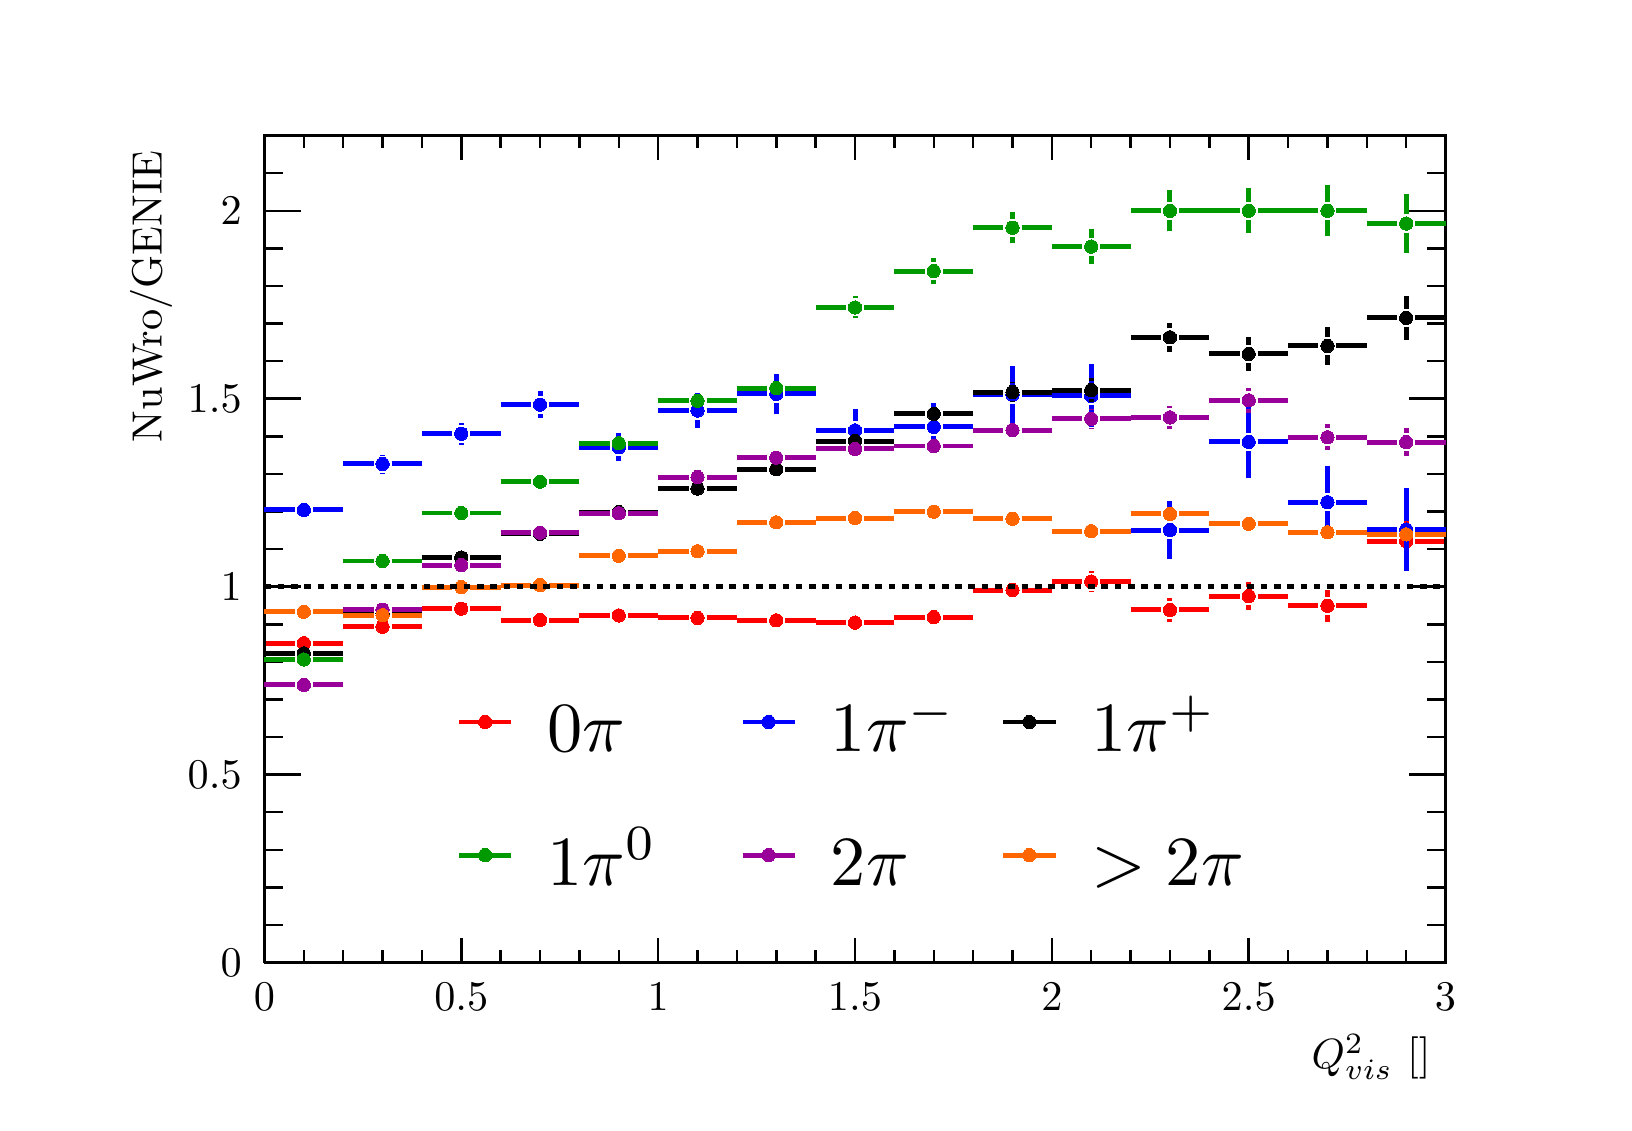
\begin{tikzpicture}
\pgfdeclareplotmark{cross} {
\pgfpathmoveto{\pgfpoint{-0.3\pgfplotmarksize}{\pgfplotmarksize}}
\pgfpathlineto{\pgfpoint{+0.3\pgfplotmarksize}{\pgfplotmarksize}}
\pgfpathlineto{\pgfpoint{+0.3\pgfplotmarksize}{0.3\pgfplotmarksize}}
\pgfpathlineto{\pgfpoint{+1\pgfplotmarksize}{0.3\pgfplotmarksize}}
\pgfpathlineto{\pgfpoint{+1\pgfplotmarksize}{-0.3\pgfplotmarksize}}
\pgfpathlineto{\pgfpoint{+0.3\pgfplotmarksize}{-0.3\pgfplotmarksize}}
\pgfpathlineto{\pgfpoint{+0.3\pgfplotmarksize}{-1.\pgfplotmarksize}}
\pgfpathlineto{\pgfpoint{-0.3\pgfplotmarksize}{-1.\pgfplotmarksize}}
\pgfpathlineto{\pgfpoint{-0.3\pgfplotmarksize}{-0.3\pgfplotmarksize}}
\pgfpathlineto{\pgfpoint{-1.\pgfplotmarksize}{-0.3\pgfplotmarksize}}
\pgfpathlineto{\pgfpoint{-1.\pgfplotmarksize}{0.3\pgfplotmarksize}}
\pgfpathlineto{\pgfpoint{-0.3\pgfplotmarksize}{0.3\pgfplotmarksize}}
\pgfpathclose
\pgfusepathqstroke
}
\pgfdeclareplotmark{cross*} {
\pgfpathmoveto{\pgfpoint{-0.3\pgfplotmarksize}{\pgfplotmarksize}}
\pgfpathlineto{\pgfpoint{+0.3\pgfplotmarksize}{\pgfplotmarksize}}
\pgfpathlineto{\pgfpoint{+0.3\pgfplotmarksize}{0.3\pgfplotmarksize}}
\pgfpathlineto{\pgfpoint{+1\pgfplotmarksize}{0.3\pgfplotmarksize}}
\pgfpathlineto{\pgfpoint{+1\pgfplotmarksize}{-0.3\pgfplotmarksize}}
\pgfpathlineto{\pgfpoint{+0.3\pgfplotmarksize}{-0.3\pgfplotmarksize}}
\pgfpathlineto{\pgfpoint{+0.3\pgfplotmarksize}{-1.\pgfplotmarksize}}
\pgfpathlineto{\pgfpoint{-0.3\pgfplotmarksize}{-1.\pgfplotmarksize}}
\pgfpathlineto{\pgfpoint{-0.3\pgfplotmarksize}{-0.3\pgfplotmarksize}}
\pgfpathlineto{\pgfpoint{-1.\pgfplotmarksize}{-0.3\pgfplotmarksize}}
\pgfpathlineto{\pgfpoint{-1.\pgfplotmarksize}{0.3\pgfplotmarksize}}
\pgfpathlineto{\pgfpoint{-0.3\pgfplotmarksize}{0.3\pgfplotmarksize}}
\pgfpathclose
\pgfusepathqfillstroke
}
\pgfdeclareplotmark{newstar} {
\pgfpathmoveto{\pgfqpoint{0pt}{\pgfplotmarksize}}
\pgfpathlineto{\pgfqpointpolar{44}{0.5\pgfplotmarksize}}
\pgfpathlineto{\pgfqpointpolar{18}{\pgfplotmarksize}}
\pgfpathlineto{\pgfqpointpolar{-20}{0.5\pgfplotmarksize}}
\pgfpathlineto{\pgfqpointpolar{-54}{\pgfplotmarksize}}
\pgfpathlineto{\pgfqpointpolar{-90}{0.5\pgfplotmarksize}}
\pgfpathlineto{\pgfqpointpolar{234}{\pgfplotmarksize}}
\pgfpathlineto{\pgfqpointpolar{198}{0.5\pgfplotmarksize}}
\pgfpathlineto{\pgfqpointpolar{162}{\pgfplotmarksize}}
\pgfpathlineto{\pgfqpointpolar{134}{0.5\pgfplotmarksize}}
\pgfpathclose
\pgfusepathqstroke
}
\pgfdeclareplotmark{newstar*} {
\pgfpathmoveto{\pgfqpoint{0pt}{\pgfplotmarksize}}
\pgfpathlineto{\pgfqpointpolar{44}{0.5\pgfplotmarksize}}
\pgfpathlineto{\pgfqpointpolar{18}{\pgfplotmarksize}}
\pgfpathlineto{\pgfqpointpolar{-20}{0.5\pgfplotmarksize}}
\pgfpathlineto{\pgfqpointpolar{-54}{\pgfplotmarksize}}
\pgfpathlineto{\pgfqpointpolar{-90}{0.5\pgfplotmarksize}}
\pgfpathlineto{\pgfqpointpolar{234}{\pgfplotmarksize}}
\pgfpathlineto{\pgfqpointpolar{198}{0.5\pgfplotmarksize}}
\pgfpathlineto{\pgfqpointpolar{162}{\pgfplotmarksize}}
\pgfpathlineto{\pgfqpointpolar{134}{0.5\pgfplotmarksize}}
\pgfpathclose
\pgfusepathqfillstroke
}
\definecolor{c}{rgb}{1,1,1};
\draw [color=c, fill=c] (0,0) rectangle (20,13.639);
\draw [color=c, fill=c] (3,1.77307) rectangle (18,12.2751);
\definecolor{c}{rgb}{0,0,0};
\draw [c,line width=0.9] (3,1.77307) -- (3,12.2751) -- (18,12.2751) -- (18,1.77307) -- (3,1.77307);
\definecolor{c}{rgb}{1,1,1};
\draw [color=c, fill=c] (3,1.77307) rectangle (18,12.2751);
\definecolor{c}{rgb}{0,0,0};
\draw [c,line width=0.9] (3,1.77307) -- (3,12.2751) -- (18,12.2751) -- (18,1.77307) -- (3,1.77307);
\definecolor{c}{rgb}{1,0,0};
\draw [c,line width=1.8] (3,5.82886) -- (3.38539,5.82886);
\draw [c,line width=1.8] (3.61461,5.82886) -- (4,5.82886);
\foreach \P in {(3.5,5.82886)}{\draw[mark options={color=c,fill=c},mark size=2.402402pt, line width=0.000000pt, mark=*] plot coordinates {\P};}
\draw [c,line width=1.8] (4,6.03849) -- (4.38539,6.03849);
\draw [c,line width=1.8] (4.61461,6.03849) -- (5,6.03849);
\foreach \P in {(4.5,6.03849)}{\draw[mark options={color=c,fill=c},mark size=2.402402pt, line width=0.000000pt, mark=*] plot coordinates {\P};}
\draw [c,line width=1.8] (5,6.26711) -- (5.38539,6.26711);
\draw [c,line width=1.8] (5.61461,6.26711) -- (6,6.26711);
\foreach \P in {(5.5,6.26711)}{\draw[mark options={color=c,fill=c},mark size=2.402402pt, line width=0.000000pt, mark=*] plot coordinates {\P};}
\draw [c,line width=1.8] (6,6.12288) -- (6.38539,6.12288);
\draw [c,line width=1.8] (6.61461,6.12288) -- (7,6.12288);
\foreach \P in {(6.5,6.12288)}{\draw[mark options={color=c,fill=c},mark size=2.402402pt, line width=0.000000pt, mark=*] plot coordinates {\P};}
\draw [c,line width=1.8] (7,6.18166) -- (7.38539,6.18166);
\draw [c,line width=1.8] (7.61461,6.18166) -- (8,6.18166);
\foreach \P in {(7.5,6.18166)}{\draw[mark options={color=c,fill=c},mark size=2.402402pt, line width=0.000000pt, mark=*] plot coordinates {\P};}
\draw [c,line width=1.8] (8,6.14986) -- (8.38539,6.14986);
\draw [c,line width=1.8] (8.61461,6.14986) -- (9,6.14986);
\foreach \P in {(8.5,6.14986)}{\draw[mark options={color=c,fill=c},mark size=2.402402pt, line width=0.000000pt, mark=*] plot coordinates {\P};}
\draw [c,line width=1.8] (9,6.11908) -- (9.38539,6.11908);
\draw [c,line width=1.8] (9.61461,6.11908) -- (10,6.11908);
\foreach \P in {(9.5,6.11908)}{\draw[mark options={color=c,fill=c},mark size=2.402402pt, line width=0.000000pt, mark=*] plot coordinates {\P};}
\draw [c,line width=1.8] (10,6.08987) -- (10.3854,6.08987);
\draw [c,line width=1.8] (10.6146,6.08987) -- (11,6.08987);
\foreach \P in {(10.5,6.08987)}{\draw[mark options={color=c,fill=c},mark size=2.402402pt, line width=0.000000pt, mark=*] plot coordinates {\P};}
\draw [c,line width=1.8] (11,6.16035) -- (11.3854,6.16035);
\draw [c,line width=1.8] (11.6146,6.16035) -- (12,6.16035);
\foreach \P in {(11.5,6.16035)}{\draw[mark options={color=c,fill=c},mark size=2.402402pt, line width=0.000000pt, mark=*] plot coordinates {\P};}
\draw [c,line width=1.8] (12,6.50381) -- (12.3854,6.50381);
\draw [c,line width=1.8] (12.6146,6.50381) -- (13,6.50381);
\foreach \P in {(12.5,6.50381)}{\draw[mark options={color=c,fill=c},mark size=2.402402pt, line width=0.000000pt, mark=*] plot coordinates {\P};}
\draw [c,line width=1.8] (13.5,6.47964) -- (13.5,6.49613);
\draw [c,line width=1.8] (13.5,6.72535) -- (13.5,6.74184);
\draw [c,line width=1.8] (13,6.61074) -- (13.3854,6.61074);
\draw [c,line width=1.8] (13.6146,6.61074) -- (14,6.61074);
\foreach \P in {(13.5,6.61074)}{\draw[mark options={color=c,fill=c},mark size=2.402402pt, line width=0.000000pt, mark=*] plot coordinates {\P};}
\draw [c,line width=1.8] (14.5,6.10391) -- (14.5,6.13613);
\draw [c,line width=1.8] (14.5,6.36536) -- (14.5,6.39759);
\draw [c,line width=1.8] (14,6.25075) -- (14.3854,6.25075);
\draw [c,line width=1.8] (14.6146,6.25075) -- (15,6.25075);
\foreach \P in {(14.5,6.25075)}{\draw[mark options={color=c,fill=c},mark size=2.402402pt, line width=0.000000pt, mark=*] plot coordinates {\P};}
\draw [c,line width=1.8] (15.5,6.25269) -- (15.5,6.31279);
\draw [c,line width=1.8] (15.5,6.54202) -- (15.5,6.60213);
\draw [c,line width=1.8] (15,6.42741) -- (15.3854,6.42741);
\draw [c,line width=1.8] (15.6146,6.42741) -- (16,6.42741);
\foreach \P in {(15.5,6.42741)}{\draw[mark options={color=c,fill=c},mark size=2.402402pt, line width=0.000000pt, mark=*] plot coordinates {\P};}
\draw [c,line width=1.8] (16.5,6.10359) -- (16.5,6.18975);
\draw [c,line width=1.8] (16.5,6.41898) -- (16.5,6.50514);
\draw [c,line width=1.8] (16,6.30436) -- (16.3854,6.30436);
\draw [c,line width=1.8] (16.6146,6.30436) -- (17,6.30436);
\foreach \P in {(16.5,6.30436)}{\draw[mark options={color=c,fill=c},mark size=2.402402pt, line width=0.000000pt, mark=*] plot coordinates {\P};}
\draw [c,line width=1.8] (17.5,6.87193) -- (17.5,7.01171);
\draw [c,line width=1.8] (17.5,7.24094) -- (17.5,7.38072);
\draw [c,line width=1.8] (17,7.12632) -- (17.3854,7.12632);
\draw [c,line width=1.8] (17.6146,7.12632) -- (18,7.12632);
\foreach \P in {(17.5,7.12632)}{\draw[mark options={color=c,fill=c},mark size=2.402402pt, line width=0.000000pt, mark=*] plot coordinates {\P};}
\definecolor{c}{rgb}{0,0,0};
\draw [c,line width=0.9] (3,1.77307) -- (18,1.77307);
\draw [c,line width=0.9] (3,2.07994) -- (3,1.77307);
\draw [c,line width=0.9] (3.5,1.9265) -- (3.5,1.77307);
\draw [c,line width=0.9] (4,1.9265) -- (4,1.77307);
\draw [c,line width=0.9] (4.5,1.9265) -- (4.5,1.77307);
\draw [c,line width=0.9] (5,1.9265) -- (5,1.77307);
\draw [c,line width=0.9] (5.5,2.07994) -- (5.5,1.77307);
\draw [c,line width=0.9] (6,1.9265) -- (6,1.77307);
\draw [c,line width=0.9] (6.5,1.9265) -- (6.5,1.77307);
\draw [c,line width=0.9] (7,1.9265) -- (7,1.77307);
\draw [c,line width=0.9] (7.5,1.9265) -- (7.5,1.77307);
\draw [c,line width=0.9] (8,2.07994) -- (8,1.77307);
\draw [c,line width=0.9] (8.5,1.9265) -- (8.5,1.77307);
\draw [c,line width=0.9] (9,1.9265) -- (9,1.77307);
\draw [c,line width=0.9] (9.5,1.9265) -- (9.5,1.77307);
\draw [c,line width=0.9] (10,1.9265) -- (10,1.77307);
\draw [c,line width=0.9] (10.5,2.07994) -- (10.5,1.77307);
\draw [c,line width=0.9] (11,1.9265) -- (11,1.77307);
\draw [c,line width=0.9] (11.5,1.9265) -- (11.5,1.77307);
\draw [c,line width=0.9] (12,1.9265) -- (12,1.77307);
\draw [c,line width=0.9] (12.5,1.9265) -- (12.5,1.77307);
\draw [c,line width=0.9] (13,2.07994) -- (13,1.77307);
\draw [c,line width=0.9] (13.5,1.9265) -- (13.5,1.77307);
\draw [c,line width=0.9] (14,1.9265) -- (14,1.77307);
\draw [c,line width=0.9] (14.5,1.9265) -- (14.5,1.77307);
\draw [c,line width=0.9] (15,1.9265) -- (15,1.77307);
\draw [c,line width=0.9] (15.5,2.07994) -- (15.5,1.77307);
\draw [c,line width=0.9] (16,1.9265) -- (16,1.77307);
\draw [c,line width=0.9] (16.5,1.9265) -- (16.5,1.77307);
\draw [c,line width=0.9] (17,1.9265) -- (17,1.77307);
\draw [c,line width=0.9] (17.5,1.9265) -- (17.5,1.77307);
\draw [c,line width=0.9] (18,2.07994) -- (18,1.77307);
\draw [c,line width=0.9] (18,2.07994) -- (18,1.77307);
\draw [anchor=base] (3,1.15931) node[scale=1.52731, color=c, rotate=0]{0};
\draw [anchor=base] (5.5,1.15931) node[scale=1.52731, color=c, rotate=0]{0.5};
\draw [anchor=base] (8,1.15931) node[scale=1.52731, color=c, rotate=0]{1};
\draw [anchor=base] (10.5,1.15931) node[scale=1.52731, color=c, rotate=0]{1.5};
\draw [anchor=base] (13,1.15931) node[scale=1.52731, color=c, rotate=0]{2};
\draw [anchor=base] (15.5,1.15931) node[scale=1.52731, color=c, rotate=0]{2.5};
\draw [anchor=base] (18,1.15931) node[scale=1.52731, color=c, rotate=0]{3};
\draw [anchor= east] (18,0.572837) node[scale=1.52731, color=c, rotate=0]{$Q^{2}_{\text{vis}}$ [\si{\giga\electronvolt\squared}] };
\draw [c,line width=0.9] (3,12.2751) -- (18,12.2751);
\draw [c,line width=0.9] (3,11.9682) -- (3,12.2751);
\draw [c,line width=0.9] (3.5,12.1216) -- (3.5,12.2751);
\draw [c,line width=0.9] (4,12.1216) -- (4,12.2751);
\draw [c,line width=0.9] (4.5,12.1216) -- (4.5,12.2751);
\draw [c,line width=0.9] (5,12.1216) -- (5,12.2751);
\draw [c,line width=0.9] (5.5,11.9682) -- (5.5,12.2751);
\draw [c,line width=0.9] (6,12.1216) -- (6,12.2751);
\draw [c,line width=0.9] (6.5,12.1216) -- (6.5,12.2751);
\draw [c,line width=0.9] (7,12.1216) -- (7,12.2751);
\draw [c,line width=0.9] (7.5,12.1216) -- (7.5,12.2751);
\draw [c,line width=0.9] (8,11.9682) -- (8,12.2751);
\draw [c,line width=0.9] (8.5,12.1216) -- (8.5,12.2751);
\draw [c,line width=0.9] (9,12.1216) -- (9,12.2751);
\draw [c,line width=0.9] (9.5,12.1216) -- (9.5,12.2751);
\draw [c,line width=0.9] (10,12.1216) -- (10,12.2751);
\draw [c,line width=0.9] (10.5,11.9682) -- (10.5,12.2751);
\draw [c,line width=0.9] (11,12.1216) -- (11,12.2751);
\draw [c,line width=0.9] (11.5,12.1216) -- (11.5,12.2751);
\draw [c,line width=0.9] (12,12.1216) -- (12,12.2751);
\draw [c,line width=0.9] (12.5,12.1216) -- (12.5,12.2751);
\draw [c,line width=0.9] (13,11.9682) -- (13,12.2751);
\draw [c,line width=0.9] (13.5,12.1216) -- (13.5,12.2751);
\draw [c,line width=0.9] (14,12.1216) -- (14,12.2751);
\draw [c,line width=0.9] (14.5,12.1216) -- (14.5,12.2751);
\draw [c,line width=0.9] (15,12.1216) -- (15,12.2751);
\draw [c,line width=0.9] (15.5,11.9682) -- (15.5,12.2751);
\draw [c,line width=0.9] (16,12.1216) -- (16,12.2751);
\draw [c,line width=0.9] (16.5,12.1216) -- (16.5,12.2751);
\draw [c,line width=0.9] (17,12.1216) -- (17,12.2751);
\draw [c,line width=0.9] (17.5,12.1216) -- (17.5,12.2751);
\draw [c,line width=0.9] (18,11.9682) -- (18,12.2751);
\draw [c,line width=0.9] (18,11.9682) -- (18,12.2751);
\draw [c,line width=0.9] (3,1.77307) -- (3,12.2751);
\draw [c,line width=0.9] (3.462,1.77307) -- (3,1.77307);
\draw [c,line width=0.9] (3.231,2.25043) -- (3,2.25043);
\draw [c,line width=0.9] (3.231,2.72779) -- (3,2.72779);
\draw [c,line width=0.9] (3.231,3.20516) -- (3,3.20516);
\draw [c,line width=0.9] (3.231,3.68252) -- (3,3.68252);
\draw [c,line width=0.9] (3.462,4.15989) -- (3,4.15989);
\draw [c,line width=0.9] (3.231,4.63725) -- (3,4.63725);
\draw [c,line width=0.9] (3.231,5.11461) -- (3,5.11461);
\draw [c,line width=0.9] (3.231,5.59198) -- (3,5.59198);
\draw [c,line width=0.9] (3.231,6.06934) -- (3,6.06934);
\draw [c,line width=0.9] (3.462,6.5467) -- (3,6.5467);
\draw [c,line width=0.9] (3.231,7.02407) -- (3,7.02407);
\draw [c,line width=0.9] (3.231,7.50143) -- (3,7.50143);
\draw [c,line width=0.9] (3.231,7.9788) -- (3,7.9788);
\draw [c,line width=0.9] (3.231,8.45616) -- (3,8.45616);
\draw [c,line width=0.9] (3.462,8.93352) -- (3,8.93352);
\draw [c,line width=0.9] (3.231,9.41089) -- (3,9.41089);
\draw [c,line width=0.9] (3.231,9.88825) -- (3,9.88825);
\draw [c,line width=0.9] (3.231,10.3656) -- (3,10.3656);
\draw [c,line width=0.9] (3.231,10.843) -- (3,10.843);
\draw [c,line width=0.9] (3.462,11.3203) -- (3,11.3203);
\draw [c,line width=0.9] (3.462,11.3203) -- (3,11.3203);
\draw [c,line width=0.9] (3.231,11.7977) -- (3,11.7977);
\draw [c,line width=0.9] (3.231,12.2751) -- (3,12.2751);
\draw [anchor= east] (2.9,1.77307) node[scale=1.52731, color=c, rotate=0]{0};
\draw [anchor= east] (2.9,4.15989) node[scale=1.52731, color=c, rotate=0]{0.5};
\draw [anchor= east] (2.9,6.5467) node[scale=1.52731, color=c, rotate=0]{1};
\draw [anchor= east] (2.9,8.93352) node[scale=1.52731, color=c, rotate=0]{1.5};
\draw [anchor= east] (2.9,11.3203) node[scale=1.52731, color=c, rotate=0]{2};
\draw [anchor= east] (1.56,12.2751) node[scale=1.52731, color=c, rotate=90]{ NuWro/GENIE};
\draw [c,line width=0.9] (18,1.77307) -- (18,12.2751);
\draw [c,line width=0.9] (17.538,1.77307) -- (18,1.77307);
\draw [c,line width=0.9] (17.769,2.25043) -- (18,2.25043);
\draw [c,line width=0.9] (17.769,2.72779) -- (18,2.72779);
\draw [c,line width=0.9] (17.769,3.20516) -- (18,3.20516);
\draw [c,line width=0.9] (17.769,3.68252) -- (18,3.68252);
\draw [c,line width=0.9] (17.538,4.15989) -- (18,4.15989);
\draw [c,line width=0.9] (17.769,4.63725) -- (18,4.63725);
\draw [c,line width=0.9] (17.769,5.11461) -- (18,5.11461);
\draw [c,line width=0.9] (17.769,5.59198) -- (18,5.59198);
\draw [c,line width=0.9] (17.769,6.06934) -- (18,6.06934);
\draw [c,line width=0.9] (17.538,6.5467) -- (18,6.5467);
\draw [c,line width=0.9] (17.769,7.02407) -- (18,7.02407);
\draw [c,line width=0.9] (17.769,7.50143) -- (18,7.50143);
\draw [c,line width=0.9] (17.769,7.9788) -- (18,7.9788);
\draw [c,line width=0.9] (17.769,8.45616) -- (18,8.45616);
\draw [c,line width=0.9] (17.538,8.93352) -- (18,8.93352);
\draw [c,line width=0.9] (17.769,9.41089) -- (18,9.41089);
\draw [c,line width=0.9] (17.769,9.88825) -- (18,9.88825);
\draw [c,line width=0.9] (17.769,10.3656) -- (18,10.3656);
\draw [c,line width=0.9] (17.769,10.843) -- (18,10.843);
\draw [c,line width=0.9] (17.538,11.3203) -- (18,11.3203);
\draw [c,line width=0.9] (17.538,11.3203) -- (18,11.3203);
\draw [c,line width=0.9] (17.769,11.7977) -- (18,11.7977);
\draw [c,line width=0.9] (17.769,12.2751) -- (18,12.2751);
\definecolor{c}{rgb}{0,0,1};
\draw [c,line width=1.8] (3,7.52061) -- (3.38539,7.52061);
\draw [c,line width=1.8] (3.61461,7.52061) -- (4,7.52061);
\foreach \P in {(3.5,7.52061)}{\draw[mark options={color=c,fill=c},mark size=2.402402pt, line width=0.000000pt, mark=*] plot coordinates {\P};}
\draw [c,line width=1.8] (4.5,7.98956) -- (4.5,7.99026);
\draw [c,line width=1.8] (4.5,8.21949) -- (4.5,8.22019);
\draw [c,line width=1.8] (4,8.10488) -- (4.38539,8.10488);
\draw [c,line width=1.8] (4.61461,8.10488) -- (5,8.10488);
\foreach \P in {(4.5,8.10488)}{\draw[mark options={color=c,fill=c},mark size=2.402402pt, line width=0.000000pt, mark=*] plot coordinates {\P};}
\draw [c,line width=1.8] (5.5,8.3504) -- (5.5,8.37484);
\draw [c,line width=1.8] (5.5,8.60406) -- (5.5,8.6285);
\draw [c,line width=1.8] (5,8.48945) -- (5.38539,8.48945);
\draw [c,line width=1.8] (5.61461,8.48945) -- (6,8.48945);
\foreach \P in {(5.5,8.48945)}{\draw[mark options={color=c,fill=c},mark size=2.402402pt, line width=0.000000pt, mark=*] plot coordinates {\P};}
\draw [c,line width=1.8] (6.5,8.68828) -- (6.5,8.74365);
\draw [c,line width=1.8] (6.5,8.97288) -- (6.5,9.02825);
\draw [c,line width=1.8] (6,8.85826) -- (6.38539,8.85826);
\draw [c,line width=1.8] (6.61461,8.85826) -- (7,8.85826);
\foreach \P in {(6.5,8.85826)}{\draw[mark options={color=c,fill=c},mark size=2.402402pt, line width=0.000000pt, mark=*] plot coordinates {\P};}
\draw [c,line width=1.8] (7.5,8.13763) -- (7.5,8.20169);
\draw [c,line width=1.8] (7.5,8.43091) -- (7.5,8.49497);
\draw [c,line width=1.8] (7,8.3163) -- (7.38539,8.3163);
\draw [c,line width=1.8] (7.61461,8.3163) -- (8,8.3163);
\foreach \P in {(7.5,8.3163)}{\draw[mark options={color=c,fill=c},mark size=2.402402pt, line width=0.000000pt, mark=*] plot coordinates {\P};}
\draw [c,line width=1.8] (8.5,8.56533) -- (8.5,8.66955);
\draw [c,line width=1.8] (8.5,8.89877) -- (8.5,9.00299);
\draw [c,line width=1.8] (8,8.78416) -- (8.38539,8.78416);
\draw [c,line width=1.8] (8.61461,8.78416) -- (9,8.78416);
\foreach \P in {(8.5,8.78416)}{\draw[mark options={color=c,fill=c},mark size=2.402402pt, line width=0.000000pt, mark=*] plot coordinates {\P};}
\draw [c,line width=1.8] (9.5,8.74004) -- (9.5,8.87982);
\draw [c,line width=1.8] (9.5,9.10905) -- (9.5,9.24883);
\draw [c,line width=1.8] (9,8.99443) -- (9.38539,8.99443);
\draw [c,line width=1.8] (9.61461,8.99443) -- (10,8.99443);
\foreach \P in {(9.5,8.99443)}{\draw[mark options={color=c,fill=c},mark size=2.402402pt, line width=0.000000pt, mark=*] plot coordinates {\P};}
\draw [c,line width=1.8] (10.5,8.25734) -- (10.5,8.41721);
\draw [c,line width=1.8] (10.5,8.64643) -- (10.5,8.8063);
\draw [c,line width=1.8] (10,8.53182) -- (10.3854,8.53182);
\draw [c,line width=1.8] (10.6146,8.53182) -- (11,8.53182);
\foreach \P in {(10.5,8.53182)}{\draw[mark options={color=c,fill=c},mark size=2.402402pt, line width=0.000000pt, mark=*] plot coordinates {\P};}
\draw [c,line width=1.8] (11.5,8.2699) -- (11.5,8.46171);
\draw [c,line width=1.8] (11.5,8.69094) -- (11.5,8.88275);
\draw [c,line width=1.8] (11,8.57632) -- (11.3854,8.57632);
\draw [c,line width=1.8] (11.6146,8.57632) -- (12,8.57632);
\foreach \P in {(11.5,8.57632)}{\draw[mark options={color=c,fill=c},mark size=2.402402pt, line width=0.000000pt, mark=*] plot coordinates {\P};}
\draw [c,line width=1.8] (12.5,8.61854) -- (12.5,8.87227);
\draw [c,line width=1.8] (12.5,9.1015) -- (12.5,9.35523);
\draw [c,line width=1.8] (12,8.98688) -- (12.3854,8.98688);
\draw [c,line width=1.8] (12.6146,8.98688) -- (13,8.98688);
\foreach \P in {(12.5,8.98688)}{\draw[mark options={color=c,fill=c},mark size=2.402402pt, line width=0.000000pt, mark=*] plot coordinates {\P};}
\draw [c,line width=1.8] (13.5,8.56917) -- (13.5,8.85412);
\draw [c,line width=1.8] (13.5,9.08334) -- (13.5,9.36829);
\draw [c,line width=1.8] (13,8.96873) -- (13.3854,8.96873);
\draw [c,line width=1.8] (13.6146,8.96873) -- (14,8.96873);
\foreach \P in {(13.5,8.96873)}{\draw[mark options={color=c,fill=c},mark size=2.402402pt, line width=0.000000pt, mark=*] plot coordinates {\P};}
\draw [c,line width=1.8] (14.5,6.89727) -- (14.5,7.15055);
\draw [c,line width=1.8] (14.5,7.37978) -- (14.5,7.63306);
\draw [c,line width=1.8] (14,7.26516) -- (14.3854,7.26516);
\draw [c,line width=1.8] (14.6146,7.26516) -- (15,7.26516);
\foreach \P in {(14.5,7.26516)}{\draw[mark options={color=c,fill=c},mark size=2.402402pt, line width=0.000000pt, mark=*] plot coordinates {\P};}
\draw [c,line width=1.8] (15.5,7.92354) -- (15.5,8.27087);
\draw [c,line width=1.8] (15.5,8.5001) -- (15.5,8.84743);
\draw [c,line width=1.8] (15,8.38549) -- (15.3854,8.38549);
\draw [c,line width=1.8] (15.6146,8.38549) -- (16,8.38549);
\foreach \P in {(15.5,8.38549)}{\draw[mark options={color=c,fill=c},mark size=2.402402pt, line width=0.000000pt, mark=*] plot coordinates {\P};}
\draw [c,line width=1.8] (16.5,7.16342) -- (16.5,7.50513);
\draw [c,line width=1.8] (16.5,7.73436) -- (16.5,8.07607);
\draw [c,line width=1.8] (16,7.61974) -- (16.3854,7.61974);
\draw [c,line width=1.8] (16.6146,7.61974) -- (17,7.61974);
\foreach \P in {(16.5,7.61974)}{\draw[mark options={color=c,fill=c},mark size=2.402402pt, line width=0.000000pt, mark=*] plot coordinates {\P};}
\draw [c,line width=1.8] (17.5,6.74312) -- (17.5,7.15648);
\draw [c,line width=1.8] (17.5,7.38571) -- (17.5,7.79908);
\draw [c,line width=1.8] (17,7.2711) -- (17.3854,7.2711);
\draw [c,line width=1.8] (17.6146,7.2711) -- (18,7.2711);
\foreach \P in {(17.5,7.2711)}{\draw[mark options={color=c,fill=c},mark size=2.402402pt, line width=0.000000pt, mark=*] plot coordinates {\P};}
\definecolor{c}{rgb}{0,0,0};
\draw [c,line width=1.8] (3,5.69971) -- (3.38539,5.69971);
\draw [c,line width=1.8] (3.61461,5.69971) -- (4,5.69971);
\foreach \P in {(3.5,5.69971)}{\draw[mark options={color=c,fill=c},mark size=2.402402pt, line width=0.000000pt, mark=*] plot coordinates {\P};}
\draw [c,line width=1.8] (4,6.20869) -- (4.38539,6.20869);
\draw [c,line width=1.8] (4.61461,6.20869) -- (5,6.20869);
\foreach \P in {(4.5,6.20869)}{\draw[mark options={color=c,fill=c},mark size=2.402402pt, line width=0.000000pt, mark=*] plot coordinates {\P};}
\draw [c,line width=1.8] (5,6.91728) -- (5.38539,6.91728);
\draw [c,line width=1.8] (5.61461,6.91728) -- (6,6.91728);
\foreach \P in {(5.5,6.91728)}{\draw[mark options={color=c,fill=c},mark size=2.402402pt, line width=0.000000pt, mark=*] plot coordinates {\P};}
\draw [c,line width=1.8] (6,7.21845) -- (6.38539,7.21845);
\draw [c,line width=1.8] (6.61461,7.21845) -- (7,7.21845);
\foreach \P in {(6.5,7.21845)}{\draw[mark options={color=c,fill=c},mark size=2.402402pt, line width=0.000000pt, mark=*] plot coordinates {\P};}
\draw [c,line width=1.8] (7,7.49374) -- (7.38539,7.49374);
\draw [c,line width=1.8] (7.61461,7.49374) -- (8,7.49374);
\foreach \P in {(7.5,7.49374)}{\draw[mark options={color=c,fill=c},mark size=2.402402pt, line width=0.000000pt, mark=*] plot coordinates {\P};}
\draw [c,line width=1.8] (8,7.79179) -- (8.38539,7.79179);
\draw [c,line width=1.8] (8.61461,7.79179) -- (9,7.79179);
\foreach \P in {(8.5,7.79179)}{\draw[mark options={color=c,fill=c},mark size=2.402402pt, line width=0.000000pt, mark=*] plot coordinates {\P};}
\draw [c,line width=1.8] (9,8.03695) -- (9.38539,8.03695);
\draw [c,line width=1.8] (9.61461,8.03695) -- (10,8.03695);
\foreach \P in {(9.5,8.03695)}{\draw[mark options={color=c,fill=c},mark size=2.402402pt, line width=0.000000pt, mark=*] plot coordinates {\P};}
\draw [c,line width=1.8] (10,8.3953) -- (10.3854,8.3953);
\draw [c,line width=1.8] (10.6146,8.3953) -- (11,8.3953);
\foreach \P in {(10.5,8.3953)}{\draw[mark options={color=c,fill=c},mark size=2.402402pt, line width=0.000000pt, mark=*] plot coordinates {\P};}
\draw [c,line width=1.8] (11,8.74131) -- (11.3854,8.74131);
\draw [c,line width=1.8] (11.6146,8.74131) -- (12,8.74131);
\foreach \P in {(11.5,8.74131)}{\draw[mark options={color=c,fill=c},mark size=2.402402pt, line width=0.000000pt, mark=*] plot coordinates {\P};}
\draw [c,line width=1.8] (12.5,8.88845) -- (12.5,8.90289);
\draw [c,line width=1.8] (12.5,9.13212) -- (12.5,9.14656);
\draw [c,line width=1.8] (12,9.01751) -- (12.3854,9.01751);
\draw [c,line width=1.8] (12.6146,9.01751) -- (13,9.01751);
\foreach \P in {(12.5,9.01751)}{\draw[mark options={color=c,fill=c},mark size=2.402402pt, line width=0.000000pt, mark=*] plot coordinates {\P};}
\draw [c,line width=1.8] (13.5,8.89535) -- (13.5,8.92859);
\draw [c,line width=1.8] (13.5,9.15782) -- (13.5,9.19107);
\draw [c,line width=1.8] (13,9.04321) -- (13.3854,9.04321);
\draw [c,line width=1.8] (13.6146,9.04321) -- (14,9.04321);
\foreach \P in {(13.5,9.04321)}{\draw[mark options={color=c,fill=c},mark size=2.402402pt, line width=0.000000pt, mark=*] plot coordinates {\P};}
\draw [c,line width=1.8] (14.5,9.52667) -- (14.5,9.59931);
\draw [c,line width=1.8] (14.5,9.82853) -- (14.5,9.90117);
\draw [c,line width=1.8] (14,9.71392) -- (14.3854,9.71392);
\draw [c,line width=1.8] (14.6146,9.71392) -- (15,9.71392);
\foreach \P in {(14.5,9.71392)}{\draw[mark options={color=c,fill=c},mark size=2.402402pt, line width=0.000000pt, mark=*] plot coordinates {\P};}
\draw [c,line width=1.8] (15.5,9.29097) -- (15.5,9.38736);
\draw [c,line width=1.8] (15.5,9.61659) -- (15.5,9.71298);
\draw [c,line width=1.8] (15,9.50198) -- (15.3854,9.50198);
\draw [c,line width=1.8] (15.6146,9.50198) -- (16,9.50198);
\foreach \P in {(15.5,9.50198)}{\draw[mark options={color=c,fill=c},mark size=2.402402pt, line width=0.000000pt, mark=*] plot coordinates {\P};}
\draw [c,line width=1.8] (16.5,9.36249) -- (16.5,9.48996);
\draw [c,line width=1.8] (16.5,9.71919) -- (16.5,9.84666);
\draw [c,line width=1.8] (16,9.60458) -- (16.3854,9.60458);
\draw [c,line width=1.8] (16.6146,9.60458) -- (17,9.60458);
\foreach \P in {(16.5,9.60458)}{\draw[mark options={color=c,fill=c},mark size=2.402402pt, line width=0.000000pt, mark=*] plot coordinates {\P};}
\draw [c,line width=1.8] (17.5,9.67941) -- (17.5,9.84565);
\draw [c,line width=1.8] (17.5,10.0749) -- (17.5,10.2411);
\draw [c,line width=1.8] (17,9.96026) -- (17.3854,9.96026);
\draw [c,line width=1.8] (17.6146,9.96026) -- (18,9.96026);
\foreach \P in {(17.5,9.96026)}{\draw[mark options={color=c,fill=c},mark size=2.402402pt, line width=0.000000pt, mark=*] plot coordinates {\P};}
\definecolor{c}{rgb}{0,0.6,0};
\draw [c,line width=1.8] (3,5.62264) -- (3.38539,5.62264);
\draw [c,line width=1.8] (3.61461,5.62264) -- (4,5.62264);
\foreach \P in {(3.5,5.62264)}{\draw[mark options={color=c,fill=c},mark size=2.402402pt, line width=0.000000pt, mark=*] plot coordinates {\P};}
\draw [c,line width=1.8] (4,6.87259) -- (4.38539,6.87259);
\draw [c,line width=1.8] (4.61461,6.87259) -- (5,6.87259);
\foreach \P in {(4.5,6.87259)}{\draw[mark options={color=c,fill=c},mark size=2.402402pt, line width=0.000000pt, mark=*] plot coordinates {\P};}
\draw [c,line width=1.8] (5,7.48218) -- (5.38539,7.48218);
\draw [c,line width=1.8] (5.61461,7.48218) -- (6,7.48218);
\foreach \P in {(5.5,7.48218)}{\draw[mark options={color=c,fill=c},mark size=2.402402pt, line width=0.000000pt, mark=*] plot coordinates {\P};}
\draw [c,line width=1.8] (6,7.87976) -- (6.38539,7.87976);
\draw [c,line width=1.8] (6.61461,7.87976) -- (7,7.87976);
\foreach \P in {(6.5,7.87976)}{\draw[mark options={color=c,fill=c},mark size=2.402402pt, line width=0.000000pt, mark=*] plot coordinates {\P};}
\draw [c,line width=1.8] (7,8.36921) -- (7.38539,8.36921);
\draw [c,line width=1.8] (7.61461,8.36921) -- (8,8.36921);
\foreach \P in {(7.5,8.36921)}{\draw[mark options={color=c,fill=c},mark size=2.402402pt, line width=0.000000pt, mark=*] plot coordinates {\P};}
\draw [c,line width=1.8] (8,8.90687) -- (8.38539,8.90687);
\draw [c,line width=1.8] (8.61461,8.90687) -- (9,8.90687);
\foreach \P in {(8.5,8.90687)}{\draw[mark options={color=c,fill=c},mark size=2.402402pt, line width=0.000000pt, mark=*] plot coordinates {\P};}
\draw [c,line width=1.8] (9,9.06858) -- (9.38539,9.06858);
\draw [c,line width=1.8] (9.61461,9.06858) -- (10,9.06858);
\foreach \P in {(9.5,9.06858)}{\draw[mark options={color=c,fill=c},mark size=2.402402pt, line width=0.000000pt, mark=*] plot coordinates {\P};}
\draw [c,line width=1.8] (10.5,9.95327) -- (10.5,9.97814);
\draw [c,line width=1.8] (10.5,10.2074) -- (10.5,10.2322);
\draw [c,line width=1.8] (10,10.0928) -- (10.3854,10.0928);
\draw [c,line width=1.8] (10.6146,10.0928) -- (11,10.0928);
\foreach \P in {(10.5,10.0928)}{\draw[mark options={color=c,fill=c},mark size=2.402402pt, line width=0.000000pt, mark=*] plot coordinates {\P};}
\draw [c,line width=1.8] (11.5,10.3892) -- (11.5,10.4409);
\draw [c,line width=1.8] (11.5,10.6701) -- (11.5,10.7218);
\draw [c,line width=1.8] (11,10.5555) -- (11.3854,10.5555);
\draw [c,line width=1.8] (11.6146,10.5555) -- (12,10.5555);
\foreach \P in {(11.5,10.5555)}{\draw[mark options={color=c,fill=c},mark size=2.402402pt, line width=0.000000pt, mark=*] plot coordinates {\P};}
\draw [c,line width=1.8] (12.5,10.9078) -- (12.5,10.9911);
\draw [c,line width=1.8] (12.5,11.2203) -- (12.5,11.3035);
\draw [c,line width=1.8] (12,11.1057) -- (12.3854,11.1057);
\draw [c,line width=1.8] (12.6146,11.1057) -- (13,11.1057);
\foreach \P in {(12.5,11.1057)}{\draw[mark options={color=c,fill=c},mark size=2.402402pt, line width=0.000000pt, mark=*] plot coordinates {\P};}
\draw [c,line width=1.8] (13.5,10.6454) -- (13.5,10.7509);
\draw [c,line width=1.8] (13.5,10.9801) -- (13.5,11.0856);
\draw [c,line width=1.8] (13,10.8655) -- (13.3854,10.8655);
\draw [c,line width=1.8] (13.6146,10.8655) -- (14,10.8655);
\foreach \P in {(13.5,10.8655)}{\draw[mark options={color=c,fill=c},mark size=2.402402pt, line width=0.000000pt, mark=*] plot coordinates {\P};}
\draw [c,line width=1.8] (14.5,11.0575) -- (14.5,11.2057);
\draw [c,line width=1.8] (14.5,11.435) -- (14.5,11.5832);
\draw [c,line width=1.8] (14,11.3203) -- (14.3854,11.3203);
\draw [c,line width=1.8] (14.6146,11.3203) -- (15,11.3203);
\foreach \P in {(14.5,11.3203)}{\draw[mark options={color=c,fill=c},mark size=2.402402pt, line width=0.000000pt, mark=*] plot coordinates {\P};}
\draw [c,line width=1.8] (15.5,11.0321) -- (15.5,11.2057);
\draw [c,line width=1.8] (15.5,11.435) -- (15.5,11.6086);
\draw [c,line width=1.8] (15,11.3203) -- (15.3854,11.3203);
\draw [c,line width=1.8] (15.6146,11.3203) -- (16,11.3203);
\foreach \P in {(15.5,11.3203)}{\draw[mark options={color=c,fill=c},mark size=2.402402pt, line width=0.000000pt, mark=*] plot coordinates {\P};}
\draw [c,line width=1.8] (16.5,10.9954) -- (16.5,11.2057);
\draw [c,line width=1.8] (16.5,11.435) -- (16.5,11.6452);
\draw [c,line width=1.8] (16,11.3203) -- (16.3854,11.3203);
\draw [c,line width=1.8] (16.6146,11.3203) -- (17,11.3203);
\foreach \P in {(16.5,11.3203)}{\draw[mark options={color=c,fill=c},mark size=2.402402pt, line width=0.000000pt, mark=*] plot coordinates {\P};}
\draw [c,line width=1.8] (17.5,10.7898) -- (17.5,11.0441);
\draw [c,line width=1.8] (17.5,11.2733) -- (17.5,11.5276);
\draw [c,line width=1.8] (17,11.1587) -- (17.3854,11.1587);
\draw [c,line width=1.8] (17.6146,11.1587) -- (18,11.1587);
\foreach \P in {(17.5,11.1587)}{\draw[mark options={color=c,fill=c},mark size=2.402402pt, line width=0.000000pt, mark=*] plot coordinates {\P};}
\definecolor{c}{rgb}{0.6,0,0.6};
\draw [c,line width=1.8] (3,5.29803) -- (3.38539,5.29803);
\draw [c,line width=1.8] (3.61461,5.29803) -- (4,5.29803);
\foreach \P in {(3.5,5.29803)}{\draw[mark options={color=c,fill=c},mark size=2.402402pt, line width=0.000000pt, mark=*] plot coordinates {\P};}
\draw [c,line width=1.8] (4,6.25471) -- (4.38539,6.25471);
\draw [c,line width=1.8] (4.61461,6.25471) -- (5,6.25471);
\foreach \P in {(4.5,6.25471)}{\draw[mark options={color=c,fill=c},mark size=2.402402pt, line width=0.000000pt, mark=*] plot coordinates {\P};}
\draw [c,line width=1.8] (5,6.82104) -- (5.38539,6.82104);
\draw [c,line width=1.8] (5.61461,6.82104) -- (6,6.82104);
\foreach \P in {(5.5,6.82104)}{\draw[mark options={color=c,fill=c},mark size=2.402402pt, line width=0.000000pt, mark=*] plot coordinates {\P};}
\draw [c,line width=1.8] (6,7.23176) -- (6.38539,7.23176);
\draw [c,line width=1.8] (6.61461,7.23176) -- (7,7.23176);
\foreach \P in {(6.5,7.23176)}{\draw[mark options={color=c,fill=c},mark size=2.402402pt, line width=0.000000pt, mark=*] plot coordinates {\P};}
\draw [c,line width=1.8] (7,7.47949) -- (7.38539,7.47949);
\draw [c,line width=1.8] (7.61461,7.47949) -- (8,7.47949);
\foreach \P in {(7.5,7.47949)}{\draw[mark options={color=c,fill=c},mark size=2.402402pt, line width=0.000000pt, mark=*] plot coordinates {\P};}
\draw [c,line width=1.8] (8,7.93804) -- (8.38539,7.93804);
\draw [c,line width=1.8] (8.61461,7.93804) -- (9,7.93804);
\foreach \P in {(8.5,7.93804)}{\draw[mark options={color=c,fill=c},mark size=2.402402pt, line width=0.000000pt, mark=*] plot coordinates {\P};}
\draw [c,line width=1.8] (9,8.18466) -- (9.38539,8.18466);
\draw [c,line width=1.8] (9.61461,8.18466) -- (10,8.18466);
\foreach \P in {(9.5,8.18466)}{\draw[mark options={color=c,fill=c},mark size=2.402402pt, line width=0.000000pt, mark=*] plot coordinates {\P};}
\draw [c,line width=1.8] (10,8.29552) -- (10.3854,8.29552);
\draw [c,line width=1.8] (10.6146,8.29552) -- (11,8.29552);
\foreach \P in {(10.5,8.29552)}{\draw[mark options={color=c,fill=c},mark size=2.402402pt, line width=0.000000pt, mark=*] plot coordinates {\P};}
\draw [c,line width=1.8] (11,8.33318) -- (11.3854,8.33318);
\draw [c,line width=1.8] (11.6146,8.33318) -- (12,8.33318);
\foreach \P in {(11.5,8.33318)}{\draw[mark options={color=c,fill=c},mark size=2.402402pt, line width=0.000000pt, mark=*] plot coordinates {\P};}
\draw [c,line width=1.8] (12,8.53473) -- (12.3854,8.53473);
\draw [c,line width=1.8] (12.6146,8.53473) -- (13,8.53473);
\foreach \P in {(12.5,8.53473)}{\draw[mark options={color=c,fill=c},mark size=2.402402pt, line width=0.000000pt, mark=*] plot coordinates {\P};}
\draw [c,line width=1.8] (13.5,8.55267) -- (13.5,8.56346);
\draw [c,line width=1.8] (13.5,8.79269) -- (13.5,8.80349);
\draw [c,line width=1.8] (13,8.67808) -- (13.3854,8.67808);
\draw [c,line width=1.8] (13.6146,8.67808) -- (14,8.67808);
\foreach \P in {(13.5,8.67808)}{\draw[mark options={color=c,fill=c},mark size=2.402402pt, line width=0.000000pt, mark=*] plot coordinates {\P};}
\draw [c,line width=1.8] (14.5,8.5553) -- (14.5,8.58192);
\draw [c,line width=1.8] (14.5,8.81115) -- (14.5,8.83777);
\draw [c,line width=1.8] (14,8.69654) -- (14.3854,8.69654);
\draw [c,line width=1.8] (14.6146,8.69654) -- (15,8.69654);
\foreach \P in {(14.5,8.69654)}{\draw[mark options={color=c,fill=c},mark size=2.402402pt, line width=0.000000pt, mark=*] plot coordinates {\P};}
\draw [c,line width=1.8] (15.5,8.75403) -- (15.5,8.79878);
\draw [c,line width=1.8] (15.5,9.02801) -- (15.5,9.07276);
\draw [c,line width=1.8] (15,8.9134) -- (15.3854,8.9134);
\draw [c,line width=1.8] (15.6146,8.9134) -- (16,8.9134);
\foreach \P in {(15.5,8.9134)}{\draw[mark options={color=c,fill=c},mark size=2.402402pt, line width=0.000000pt, mark=*] plot coordinates {\P};}
\draw [c,line width=1.8] (16.5,8.27974) -- (16.5,8.32909);
\draw [c,line width=1.8] (16.5,8.55832) -- (16.5,8.60766);
\draw [c,line width=1.8] (16,8.4437) -- (16.3854,8.4437);
\draw [c,line width=1.8] (16.6146,8.4437) -- (17,8.4437);
\foreach \P in {(16.5,8.4437)}{\draw[mark options={color=c,fill=c},mark size=2.402402pt, line width=0.000000pt, mark=*] plot coordinates {\P};}
\draw [c,line width=1.8] (17.5,8.20299) -- (17.5,8.26778);
\draw [c,line width=1.8] (17.5,8.497) -- (17.5,8.56178);
\draw [c,line width=1.8] (17,8.38239) -- (17.3854,8.38239);
\draw [c,line width=1.8] (17.6146,8.38239) -- (18,8.38239);
\foreach \P in {(17.5,8.38239)}{\draw[mark options={color=c,fill=c},mark size=2.402402pt, line width=0.000000pt, mark=*] plot coordinates {\P};}
\definecolor{c}{rgb}{1,0.4,0};
\draw [c,line width=1.8] (3,6.22772) -- (3.38539,6.22772);
\draw [c,line width=1.8] (3.61461,6.22772) -- (4,6.22772);
\foreach \P in {(3.5,6.22772)}{\draw[mark options={color=c,fill=c},mark size=2.402402pt, line width=0.000000pt, mark=*] plot coordinates {\P};}
\draw [c,line width=1.8] (4,6.1851) -- (4.38539,6.1851);
\draw [c,line width=1.8] (4.61461,6.1851) -- (5,6.1851);
\foreach \P in {(4.5,6.1851)}{\draw[mark options={color=c,fill=c},mark size=2.402402pt, line width=0.000000pt, mark=*] plot coordinates {\P};}
\draw [c,line width=1.8] (5,6.5416) -- (5.38539,6.5416);
\draw [c,line width=1.8] (5.61461,6.5416) -- (6,6.5416);
\foreach \P in {(5.5,6.5416)}{\draw[mark options={color=c,fill=c},mark size=2.402402pt, line width=0.000000pt, mark=*] plot coordinates {\P};}
\draw [c,line width=1.8] (6,6.56632) -- (6.38539,6.56632);
\draw [c,line width=1.8] (6.61461,6.56632) -- (7,6.56632);
\foreach \P in {(6.5,6.56632)}{\draw[mark options={color=c,fill=c},mark size=2.402402pt, line width=0.000000pt, mark=*] plot coordinates {\P};}
\draw [c,line width=1.8] (7,6.93934) -- (7.38539,6.93934);
\draw [c,line width=1.8] (7.61461,6.93934) -- (8,6.93934);
\foreach \P in {(7.5,6.93934)}{\draw[mark options={color=c,fill=c},mark size=2.402402pt, line width=0.000000pt, mark=*] plot coordinates {\P};}
\draw [c,line width=1.8] (8,6.99683) -- (8.38539,6.99683);
\draw [c,line width=1.8] (8.61461,6.99683) -- (9,6.99683);
\foreach \P in {(8.5,6.99683)}{\draw[mark options={color=c,fill=c},mark size=2.402402pt, line width=0.000000pt, mark=*] plot coordinates {\P};}
\draw [c,line width=1.8] (9,7.36404) -- (9.38539,7.36404);
\draw [c,line width=1.8] (9.61461,7.36404) -- (10,7.36404);
\foreach \P in {(9.5,7.36404)}{\draw[mark options={color=c,fill=c},mark size=2.402402pt, line width=0.000000pt, mark=*] plot coordinates {\P};}
\draw [c,line width=1.8] (10,7.41745) -- (10.3854,7.41745);
\draw [c,line width=1.8] (10.6146,7.41745) -- (11,7.41745);
\foreach \P in {(10.5,7.41745)}{\draw[mark options={color=c,fill=c},mark size=2.402402pt, line width=0.000000pt, mark=*] plot coordinates {\P};}
\draw [c,line width=1.8] (11,7.49879) -- (11.3854,7.49879);
\draw [c,line width=1.8] (11.6146,7.49879) -- (12,7.49879);
\foreach \P in {(11.5,7.49879)}{\draw[mark options={color=c,fill=c},mark size=2.402402pt, line width=0.000000pt, mark=*] plot coordinates {\P};}
\draw [c,line width=1.8] (12,7.40886) -- (12.3854,7.40886);
\draw [c,line width=1.8] (12.6146,7.40886) -- (13,7.40886);
\foreach \P in {(12.5,7.40886)}{\draw[mark options={color=c,fill=c},mark size=2.402402pt, line width=0.000000pt, mark=*] plot coordinates {\P};}
\draw [c,line width=1.8] (13,7.25159) -- (13.3854,7.25159);
\draw [c,line width=1.8] (13.6146,7.25159) -- (14,7.25159);
\foreach \P in {(13.5,7.25159)}{\draw[mark options={color=c,fill=c},mark size=2.402402pt, line width=0.000000pt, mark=*] plot coordinates {\P};}
\draw [c,line width=1.8] (14,7.46979) -- (14.3854,7.46979);
\draw [c,line width=1.8] (14.6146,7.46979) -- (15,7.46979);
\foreach \P in {(14.5,7.46979)}{\draw[mark options={color=c,fill=c},mark size=2.402402pt, line width=0.000000pt, mark=*] plot coordinates {\P};}
\draw [c,line width=1.8] (15,7.34605) -- (15.3854,7.34605);
\draw [c,line width=1.8] (15.6146,7.34605) -- (16,7.34605);
\foreach \P in {(15.5,7.34605)}{\draw[mark options={color=c,fill=c},mark size=2.402402pt, line width=0.000000pt, mark=*] plot coordinates {\P};}
\draw [c,line width=1.8] (16,7.23807) -- (16.3854,7.23807);
\draw [c,line width=1.8] (16.6146,7.23807) -- (17,7.23807);
\foreach \P in {(16.5,7.23807)}{\draw[mark options={color=c,fill=c},mark size=2.402402pt, line width=0.000000pt, mark=*] plot coordinates {\P};}
\draw [c,line width=1.8] (17,7.21094) -- (17.3854,7.21094);
\draw [c,line width=1.8] (17.6146,7.21094) -- (18,7.21094);
\foreach \P in {(17.5,7.21094)}{\draw[mark options={color=c,fill=c},mark size=2.402402pt, line width=0.000000pt, mark=*] plot coordinates {\P};}
\definecolor{c}{rgb}{0,0,0};
\draw [c,dash pattern=on 2.40pt off 2.40pt ,line width=1.8] (3,6.5467) -- (18,6.5467);
\definecolor{c}{rgb}{1,1,1};
\draw [color=c, fill=c] (2,12.8206) rectangle (18,13.5708);
\definecolor{c}{rgb}{0,0,0};
%\draw (10,13.1957) node[scale=1.40004, color=c, rotate=0]{$0\pi$};
\definecolor{c}{rgb}{1,1,1};
\draw [color=c, fill=c] (5.32951,2.29226) rectangle (16.7049,5.67335);
\definecolor{c}{rgb}{0,0,0};
\draw [anchor=base west] (6.27746,4.44771) node[scale=2.54552, color=c, rotate=0]{$0\pi$};
\definecolor{c}{rgb}{1,1,1};
\draw [c, fill=c] (5.4717,4.23639) -- (6.13527,4.23639) -- (6.13527,5.41977) -- (5.4717,5.41977);
\definecolor{c}{rgb}{1,0,0};
\draw [c,line width=1.8] (5.4717,4.82808) -- (6.13527,4.82808);
\foreach \P in {(5.80349,4.82808)}{\draw[mark options={color=c,fill=c},mark size=2.402402pt, line width=0.000000pt, mark=*] plot coordinates {\P};}
\definecolor{c}{rgb}{0,0,0};
\draw [anchor=base west] (9.87709,4.44771) node[scale=2.54552, color=c, rotate=0]{$1\pi^{-}$};
\definecolor{c}{rgb}{1,1,1};
\draw [c, fill=c] (9.07134,4.23639) -- (9.7349,4.23639) -- (9.7349,5.41977) -- (9.07134,5.41977);
\definecolor{c}{rgb}{0,0,1};
\draw [c,line width=1.8] (9.07134,4.82808) -- (9.7349,4.82808);
\foreach \P in {(9.40312,4.82808)}{\draw[mark options={color=c,fill=c},mark size=2.402402pt, line width=0.000000pt, mark=*] plot coordinates {\P};}
\definecolor{c}{rgb}{0,0,0};
\draw [anchor=base west] (13.1885,4.44771) node[scale=2.54552, color=c, rotate=0]{$1\pi^{+}$};
\definecolor{c}{rgb}{1,1,1};
\draw [c, fill=c] (12.3827,4.23639) -- (13.0463,4.23639) -- (13.0463,5.41977) -- (12.3827,5.41977);
\definecolor{c}{rgb}{0,0,0};
\draw [c,line width=1.8] (12.3827,4.82808) -- (13.0463,4.82808);
\foreach \P in {(12.7145,4.82808)}{\draw[mark options={color=c,fill=c},mark size=2.402402pt, line width=0.000000pt, mark=*] plot coordinates {\P};}
\draw [anchor=base west] (6.27746,2.75716) node[scale=2.54552, color=c, rotate=0]{$1\pi^{0}$};
\definecolor{c}{rgb}{1,1,1};
\draw [c, fill=c] (5.4717,2.54585) -- (6.13527,2.54585) -- (6.13527,3.72923) -- (5.4717,3.72923);
\definecolor{c}{rgb}{0,0.6,0};
\draw [c,line width=1.8] (5.4717,3.13754) -- (6.13527,3.13754);
\foreach \P in {(5.80349,3.13754)}{\draw[mark options={color=c,fill=c},mark size=2.402402pt, line width=0.000000pt, mark=*] plot coordinates {\P};}
\definecolor{c}{rgb}{0,0,0};
\draw [anchor=base west] (9.87709,2.75716) node[scale=2.54552, color=c, rotate=0]{$2\pi$};
\definecolor{c}{rgb}{1,1,1};
\draw [c, fill=c] (9.07134,2.54585) -- (9.7349,2.54585) -- (9.7349,3.72923) -- (9.07134,3.72923);
\definecolor{c}{rgb}{0.6,0,0.6};
\draw [c,line width=1.8] (9.07134,3.13754) -- (9.7349,3.13754);
\foreach \P in {(9.40312,3.13754)}{\draw[mark options={color=c,fill=c},mark size=2.402402pt, line width=0.000000pt, mark=*] plot coordinates {\P};}
\definecolor{c}{rgb}{0,0,0};
\draw [anchor=base west] (13.1885,2.75716) node[scale=2.54552, color=c, rotate=0]{$>2\pi$};
\definecolor{c}{rgb}{1,1,1};
\draw [c, fill=c] (12.3827,2.54585) -- (13.0463,2.54585) -- (13.0463,3.72923) -- (12.3827,3.72923);
\definecolor{c}{rgb}{1,0.4,0};
\draw [c,line width=1.8] (12.3827,3.13754) -- (13.0463,3.13754);
\foreach \P in {(12.7145,3.13754)}{\draw[mark options={color=c,fill=c},mark size=2.402402pt, line width=0.000000pt, mark=*] plot coordinates {\P};}
\end{tikzpicture}

 		\end{adjustbox}
 	\end{minipage}
 	\caption[Comparison of NuWro and GENIE in $Q^{2}_{\textrm{vis}}$ for FHC]{Ratio of NuWro to GENIE event rates in ND-GAr as a function of $Q^{2}_{\textrm{vis}}$ with the beam in FHC mode. Left: Reconstructed selection. Right: True selection.}
 	\label{fig:Q2CompFhc}
\end{figure}

\begin{figure}[h]
	\begin{minipage}[t]{.5\linewidth}
		\begin{adjustbox}{max totalsize=\linewidth, center}
			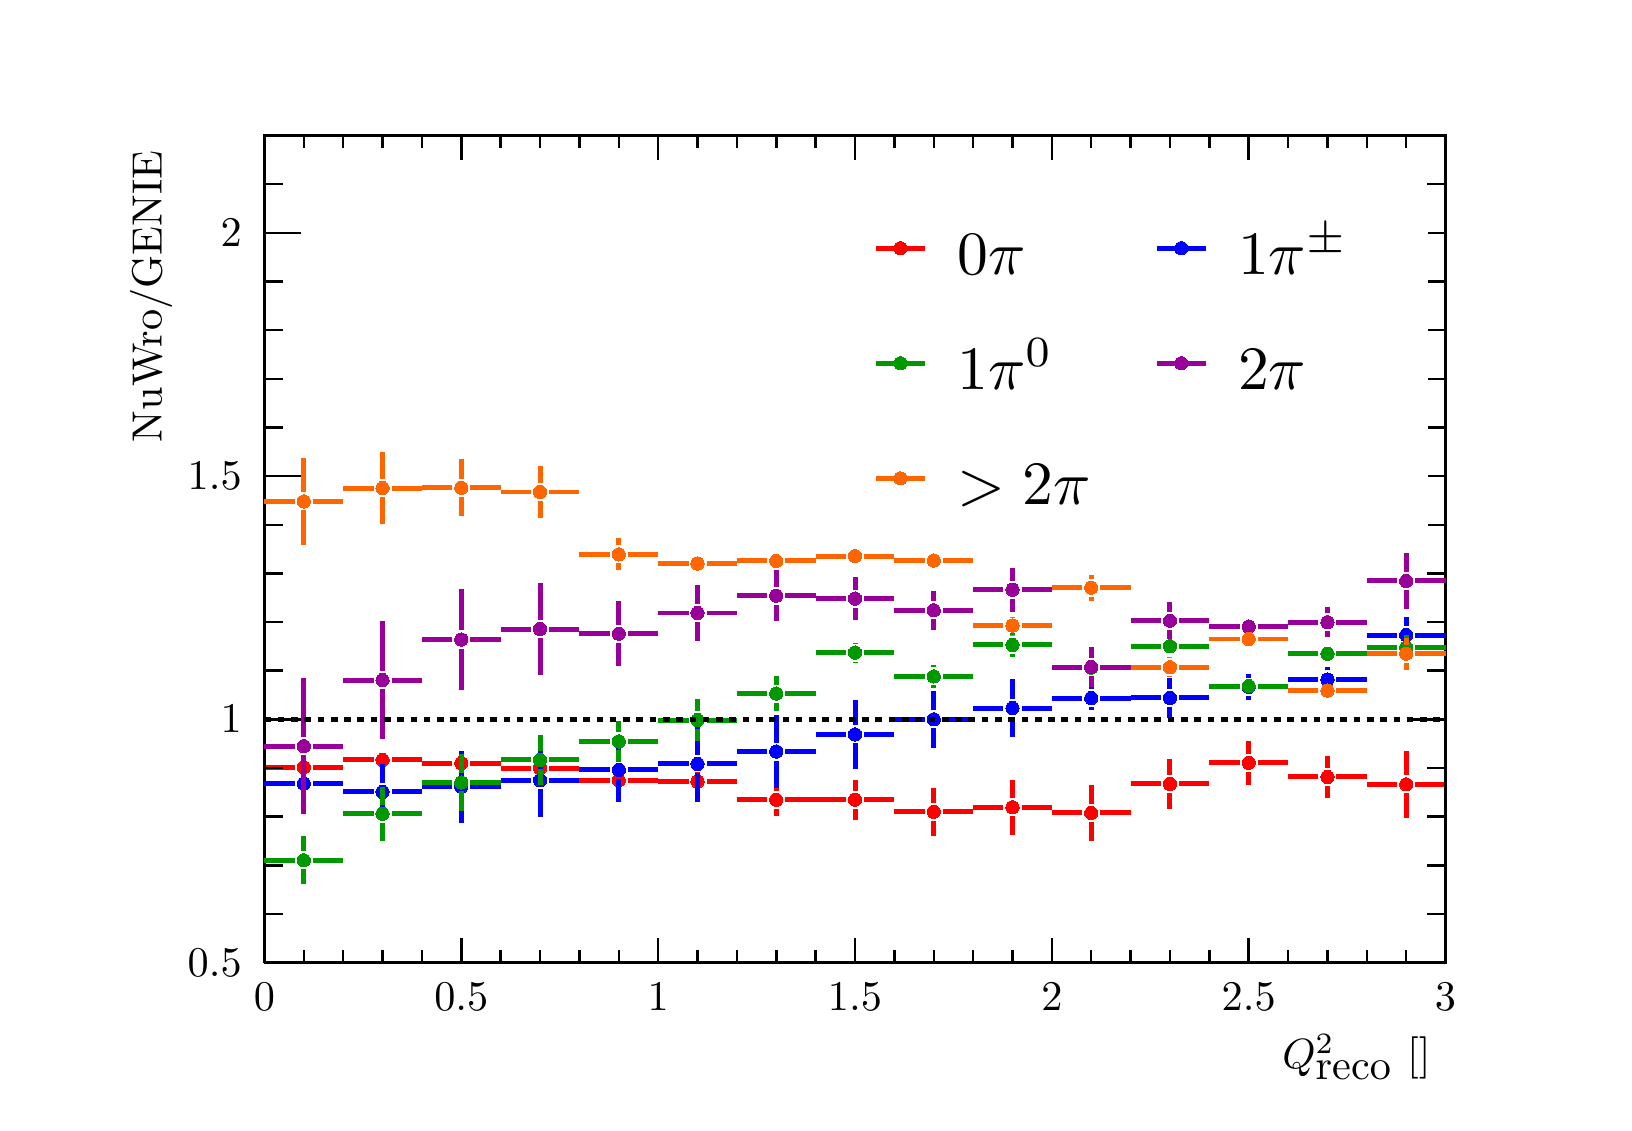
\begin{tikzpicture} 
\pgfdeclareplotmark{cross} {
\pgfpathmoveto{\pgfpoint{-0.3\pgfplotmarksize}{\pgfplotmarksize}}
\pgfpathlineto{\pgfpoint{+0.3\pgfplotmarksize}{\pgfplotmarksize}}
\pgfpathlineto{\pgfpoint{+0.3\pgfplotmarksize}{0.3\pgfplotmarksize}}
\pgfpathlineto{\pgfpoint{+1\pgfplotmarksize}{0.3\pgfplotmarksize}}
\pgfpathlineto{\pgfpoint{+1\pgfplotmarksize}{-0.3\pgfplotmarksize}}
\pgfpathlineto{\pgfpoint{+0.3\pgfplotmarksize}{-0.3\pgfplotmarksize}}
\pgfpathlineto{\pgfpoint{+0.3\pgfplotmarksize}{-1.\pgfplotmarksize}}
\pgfpathlineto{\pgfpoint{-0.3\pgfplotmarksize}{-1.\pgfplotmarksize}}
\pgfpathlineto{\pgfpoint{-0.3\pgfplotmarksize}{-0.3\pgfplotmarksize}}
\pgfpathlineto{\pgfpoint{-1.\pgfplotmarksize}{-0.3\pgfplotmarksize}}
\pgfpathlineto{\pgfpoint{-1.\pgfplotmarksize}{0.3\pgfplotmarksize}}
\pgfpathlineto{\pgfpoint{-0.3\pgfplotmarksize}{0.3\pgfplotmarksize}}
\pgfpathclose
\pgfusepathqstroke
}
\pgfdeclareplotmark{cross*} {
\pgfpathmoveto{\pgfpoint{-0.3\pgfplotmarksize}{\pgfplotmarksize}}
\pgfpathlineto{\pgfpoint{+0.3\pgfplotmarksize}{\pgfplotmarksize}}
\pgfpathlineto{\pgfpoint{+0.3\pgfplotmarksize}{0.3\pgfplotmarksize}}
\pgfpathlineto{\pgfpoint{+1\pgfplotmarksize}{0.3\pgfplotmarksize}}
\pgfpathlineto{\pgfpoint{+1\pgfplotmarksize}{-0.3\pgfplotmarksize}}
\pgfpathlineto{\pgfpoint{+0.3\pgfplotmarksize}{-0.3\pgfplotmarksize}}
\pgfpathlineto{\pgfpoint{+0.3\pgfplotmarksize}{-1.\pgfplotmarksize}}
\pgfpathlineto{\pgfpoint{-0.3\pgfplotmarksize}{-1.\pgfplotmarksize}}
\pgfpathlineto{\pgfpoint{-0.3\pgfplotmarksize}{-0.3\pgfplotmarksize}}
\pgfpathlineto{\pgfpoint{-1.\pgfplotmarksize}{-0.3\pgfplotmarksize}}
\pgfpathlineto{\pgfpoint{-1.\pgfplotmarksize}{0.3\pgfplotmarksize}}
\pgfpathlineto{\pgfpoint{-0.3\pgfplotmarksize}{0.3\pgfplotmarksize}}
\pgfpathclose
\pgfusepathqfillstroke
}
\pgfdeclareplotmark{newstar} {
\pgfpathmoveto{\pgfqpoint{0pt}{\pgfplotmarksize}}
\pgfpathlineto{\pgfqpointpolar{44}{0.5\pgfplotmarksize}}
\pgfpathlineto{\pgfqpointpolar{18}{\pgfplotmarksize}}
\pgfpathlineto{\pgfqpointpolar{-20}{0.5\pgfplotmarksize}}
\pgfpathlineto{\pgfqpointpolar{-54}{\pgfplotmarksize}}
\pgfpathlineto{\pgfqpointpolar{-90}{0.5\pgfplotmarksize}}
\pgfpathlineto{\pgfqpointpolar{234}{\pgfplotmarksize}}
\pgfpathlineto{\pgfqpointpolar{198}{0.5\pgfplotmarksize}}
\pgfpathlineto{\pgfqpointpolar{162}{\pgfplotmarksize}}
\pgfpathlineto{\pgfqpointpolar{134}{0.5\pgfplotmarksize}}
\pgfpathclose
\pgfusepathqstroke
}
\pgfdeclareplotmark{newstar*} {
\pgfpathmoveto{\pgfqpoint{0pt}{\pgfplotmarksize}}
\pgfpathlineto{\pgfqpointpolar{44}{0.5\pgfplotmarksize}}
\pgfpathlineto{\pgfqpointpolar{18}{\pgfplotmarksize}}
\pgfpathlineto{\pgfqpointpolar{-20}{0.5\pgfplotmarksize}}
\pgfpathlineto{\pgfqpointpolar{-54}{\pgfplotmarksize}}
\pgfpathlineto{\pgfqpointpolar{-90}{0.5\pgfplotmarksize}}
\pgfpathlineto{\pgfqpointpolar{234}{\pgfplotmarksize}}
\pgfpathlineto{\pgfqpointpolar{198}{0.5\pgfplotmarksize}}
\pgfpathlineto{\pgfqpointpolar{162}{\pgfplotmarksize}}
\pgfpathlineto{\pgfqpointpolar{134}{0.5\pgfplotmarksize}}
\pgfpathclose
\pgfusepathqfillstroke
}
\definecolor{c}{rgb}{1,1,1};
\draw [color=c, fill=c] (0,0) rectangle (20,13.639);
\draw [color=c, fill=c] (3,1.77307) rectangle (18,12.2751);
\definecolor{c}{rgb}{0,0,0};
\draw [c,line width=0.9] (3,1.77307) -- (3,12.2751) -- (18,12.2751) -- (18,1.77307) -- (3,1.77307);
\definecolor{c}{rgb}{1,1,1};
\draw [color=c, fill=c] (3,1.77307) rectangle (18,12.2751);
\definecolor{c}{rgb}{0,0,0};
\draw [c,line width=0.9] (3,1.77307) -- (3,12.2751) -- (18,12.2751) -- (18,1.77307) -- (3,1.77307);
\definecolor{c}{rgb}{1,0,0};
\draw [c,line width=1.8] (3,4.25421) -- (3.38539,4.25421);
\draw [c,line width=1.8] (3.61461,4.25421) -- (4,4.25421);
\foreach \P in {(3.5,4.25421)}{\draw[mark options={color=c,fill=c},mark size=2.402402pt, line width=0.000000pt, mark=*] plot coordinates {\P};}
\draw [c,line width=1.8] (4,4.34567) -- (4.38539,4.34567);
\draw [c,line width=1.8] (4.61461,4.34567) -- (5,4.34567);
\foreach \P in {(4.5,4.34567)}{\draw[mark options={color=c,fill=c},mark size=2.402402pt, line width=0.000000pt, mark=*] plot coordinates {\P};}
\draw [c,line width=1.8] (5,4.30631) -- (5.38539,4.30631);
\draw [c,line width=1.8] (5.61461,4.30631) -- (6,4.30631);
\foreach \P in {(5.5,4.30631)}{\draw[mark options={color=c,fill=c},mark size=2.402402pt, line width=0.000000pt, mark=*] plot coordinates {\P};}
\draw [c,line width=1.8] (6,4.24171) -- (6.38539,4.24171);
\draw [c,line width=1.8] (6.61461,4.24171) -- (7,4.24171);
\foreach \P in {(6.5,4.24171)}{\draw[mark options={color=c,fill=c},mark size=2.402402pt, line width=0.000000pt, mark=*] plot coordinates {\P};}
\draw [c,line width=1.8] (7,4.08889) -- (7.38539,4.08889);
\draw [c,line width=1.8] (7.61461,4.08889) -- (8,4.08889);
\foreach \P in {(7.5,4.08889)}{\draw[mark options={color=c,fill=c},mark size=2.402402pt, line width=0.000000pt, mark=*] plot coordinates {\P};}
\draw [c,line width=1.8] (8.5,3.95128) -- (8.5,3.95761);
\draw [c,line width=1.8] (8.5,4.18684) -- (8.5,4.19317);
\draw [c,line width=1.8] (8,4.07222) -- (8.38539,4.07222);
\draw [c,line width=1.8] (8.61461,4.07222) -- (9,4.07222);
\foreach \P in {(8.5,4.07222)}{\draw[mark options={color=c,fill=c},mark size=2.402402pt, line width=0.000000pt, mark=*] plot coordinates {\P};}
\draw [c,line width=1.8] (9.5,3.63206) -- (9.5,3.72656);
\draw [c,line width=1.8] (9.5,3.95578) -- (9.5,4.05028);
\draw [c,line width=1.8] (9,3.84117) -- (9.38539,3.84117);
\draw [c,line width=1.8] (9.61461,3.84117) -- (10,3.84117);
\foreach \P in {(9.5,3.84117)}{\draw[mark options={color=c,fill=c},mark size=2.402402pt, line width=0.000000pt, mark=*] plot coordinates {\P};}
\draw [c,line width=1.8] (10.5,3.58793) -- (10.5,3.72697);
\draw [c,line width=1.8] (10.5,3.9562) -- (10.5,4.09523);
\draw [c,line width=1.8] (10,3.84158) -- (10.3854,3.84158);
\draw [c,line width=1.8] (10.6146,3.84158) -- (11,3.84158);
\foreach \P in {(10.5,3.84158)}{\draw[mark options={color=c,fill=c},mark size=2.402402pt, line width=0.000000pt, mark=*] plot coordinates {\P};}
\draw [c,line width=1.8] (11.5,3.38105) -- (11.5,3.57398);
\draw [c,line width=1.8] (11.5,3.8032) -- (11.5,3.99612);
\draw [c,line width=1.8] (11,3.68859) -- (11.3854,3.68859);
\draw [c,line width=1.8] (11.6146,3.68859) -- (12,3.68859);
\foreach \P in {(11.5,3.68859)}{\draw[mark options={color=c,fill=c},mark size=2.402402pt, line width=0.000000pt, mark=*] plot coordinates {\P};}
\draw [c,line width=1.8] (12.5,3.39304) -- (12.5,3.62991);
\draw [c,line width=1.8] (12.5,3.85914) -- (12.5,4.09601);
\draw [c,line width=1.8] (12,3.74452) -- (12.3854,3.74452);
\draw [c,line width=1.8] (12.6146,3.74452) -- (13,3.74452);
\foreach \P in {(12.5,3.74452)}{\draw[mark options={color=c,fill=c},mark size=2.402402pt, line width=0.000000pt, mark=*] plot coordinates {\P};}
\draw [c,line width=1.8] (13.5,3.31572) -- (13.5,3.55841);
\draw [c,line width=1.8] (13.5,3.78764) -- (13.5,4.03034);
\draw [c,line width=1.8] (13,3.67303) -- (13.3854,3.67303);
\draw [c,line width=1.8] (13.6146,3.67303) -- (14,3.67303);
\foreach \P in {(13.5,3.67303)}{\draw[mark options={color=c,fill=c},mark size=2.402402pt, line width=0.000000pt, mark=*] plot coordinates {\P};}
\draw [c,line width=1.8] (14.5,3.72735) -- (14.5,3.92631);
\draw [c,line width=1.8] (14.5,4.15553) -- (14.5,4.35448);
\draw [c,line width=1.8] (14,4.04092) -- (14.3854,4.04092);
\draw [c,line width=1.8] (14.6146,4.04092) -- (15,4.04092);
\foreach \P in {(14.5,4.04092)}{\draw[mark options={color=c,fill=c},mark size=2.402402pt, line width=0.000000pt, mark=*] plot coordinates {\P};}
\draw [c,line width=1.8] (15.5,4.02951) -- (15.5,4.19558);
\draw [c,line width=1.8] (15.5,4.42481) -- (15.5,4.59088);
\draw [c,line width=1.8] (15,4.3102) -- (15.3854,4.3102);
\draw [c,line width=1.8] (15.6146,4.3102) -- (16,4.3102);
\foreach \P in {(15.5,4.3102)}{\draw[mark options={color=c,fill=c},mark size=2.402402pt, line width=0.000000pt, mark=*] plot coordinates {\P};}
\draw [c,line width=1.8] (16.5,3.85896) -- (16.5,4.01508);
\draw [c,line width=1.8] (16.5,4.24431) -- (16.5,4.40042);
\draw [c,line width=1.8] (16,4.12969) -- (16.3854,4.12969);
\draw [c,line width=1.8] (16.6146,4.12969) -- (17,4.12969);
\foreach \P in {(16.5,4.12969)}{\draw[mark options={color=c,fill=c},mark size=2.402402pt, line width=0.000000pt, mark=*] plot coordinates {\P};}
\draw [c,line width=1.8] (17.5,3.61236) -- (17.5,3.92183);
\draw [c,line width=1.8] (17.5,4.15105) -- (17.5,4.46052);
\draw [c,line width=1.8] (17,4.03644) -- (17.3854,4.03644);
\draw [c,line width=1.8] (17.6146,4.03644) -- (18,4.03644);
\foreach \P in {(17.5,4.03644)}{\draw[mark options={color=c,fill=c},mark size=2.402402pt, line width=0.000000pt, mark=*] plot coordinates {\P};}
\definecolor{c}{rgb}{0,0,0};
\draw [c,line width=0.9] (3,1.77307) -- (18,1.77307);
\draw [c,line width=0.9] (3,2.07994) -- (3,1.77307);
\draw [c,line width=0.9] (3.5,1.9265) -- (3.5,1.77307);
\draw [c,line width=0.9] (4,1.9265) -- (4,1.77307);
\draw [c,line width=0.9] (4.5,1.9265) -- (4.5,1.77307);
\draw [c,line width=0.9] (5,1.9265) -- (5,1.77307);
\draw [c,line width=0.9] (5.5,2.07994) -- (5.5,1.77307);
\draw [c,line width=0.9] (6,1.9265) -- (6,1.77307);
\draw [c,line width=0.9] (6.5,1.9265) -- (6.5,1.77307);
\draw [c,line width=0.9] (7,1.9265) -- (7,1.77307);
\draw [c,line width=0.9] (7.5,1.9265) -- (7.5,1.77307);
\draw [c,line width=0.9] (8,2.07994) -- (8,1.77307);
\draw [c,line width=0.9] (8.5,1.9265) -- (8.5,1.77307);
\draw [c,line width=0.9] (9,1.9265) -- (9,1.77307);
\draw [c,line width=0.9] (9.5,1.9265) -- (9.5,1.77307);
\draw [c,line width=0.9] (10,1.9265) -- (10,1.77307);
\draw [c,line width=0.9] (10.5,2.07994) -- (10.5,1.77307);
\draw [c,line width=0.9] (11,1.9265) -- (11,1.77307);
\draw [c,line width=0.9] (11.5,1.9265) -- (11.5,1.77307);
\draw [c,line width=0.9] (12,1.9265) -- (12,1.77307);
\draw [c,line width=0.9] (12.5,1.9265) -- (12.5,1.77307);
\draw [c,line width=0.9] (13,2.07994) -- (13,1.77307);
\draw [c,line width=0.9] (13.5,1.9265) -- (13.5,1.77307);
\draw [c,line width=0.9] (14,1.9265) -- (14,1.77307);
\draw [c,line width=0.9] (14.5,1.9265) -- (14.5,1.77307);
\draw [c,line width=0.9] (15,1.9265) -- (15,1.77307);
\draw [c,line width=0.9] (15.5,2.07994) -- (15.5,1.77307);
\draw [c,line width=0.9] (16,1.9265) -- (16,1.77307);
\draw [c,line width=0.9] (16.5,1.9265) -- (16.5,1.77307);
\draw [c,line width=0.9] (17,1.9265) -- (17,1.77307);
\draw [c,line width=0.9] (17.5,1.9265) -- (17.5,1.77307);
\draw [c,line width=0.9] (18,2.07994) -- (18,1.77307);
\draw [c,line width=0.9] (18,2.07994) -- (18,1.77307);
\draw [anchor=base] (3,1.15931) node[scale=1.52731, color=c, rotate=0]{0};
\draw [anchor=base] (5.5,1.15931) node[scale=1.52731, color=c, rotate=0]{0.5};
\draw [anchor=base] (8,1.15931) node[scale=1.52731, color=c, rotate=0]{1};
\draw [anchor=base] (10.5,1.15931) node[scale=1.52731, color=c, rotate=0]{1.5};
\draw [anchor=base] (13,1.15931) node[scale=1.52731, color=c, rotate=0]{2};
\draw [anchor=base] (15.5,1.15931) node[scale=1.52731, color=c, rotate=0]{2.5};
\draw [anchor=base] (18,1.15931) node[scale=1.52731, color=c, rotate=0]{3};
\draw [anchor= east] (18,0.572837) node[scale=1.52731, color=c, rotate=0]{$Q^{2}_{\textrm{reco}}$ [\si{\GeV\squared}] };
\draw [c,line width=0.9] (3,12.2751) -- (18,12.2751);
\draw [c,line width=0.9] (3,11.9682) -- (3,12.2751);
\draw [c,line width=0.9] (3.5,12.1216) -- (3.5,12.2751);
\draw [c,line width=0.9] (4,12.1216) -- (4,12.2751);
\draw [c,line width=0.9] (4.5,12.1216) -- (4.5,12.2751);
\draw [c,line width=0.9] (5,12.1216) -- (5,12.2751);
\draw [c,line width=0.9] (5.5,11.9682) -- (5.5,12.2751);
\draw [c,line width=0.9] (6,12.1216) -- (6,12.2751);
\draw [c,line width=0.9] (6.5,12.1216) -- (6.5,12.2751);
\draw [c,line width=0.9] (7,12.1216) -- (7,12.2751);
\draw [c,line width=0.9] (7.5,12.1216) -- (7.5,12.2751);
\draw [c,line width=0.9] (8,11.9682) -- (8,12.2751);
\draw [c,line width=0.9] (8.5,12.1216) -- (8.5,12.2751);
\draw [c,line width=0.9] (9,12.1216) -- (9,12.2751);
\draw [c,line width=0.9] (9.5,12.1216) -- (9.5,12.2751);
\draw [c,line width=0.9] (10,12.1216) -- (10,12.2751);
\draw [c,line width=0.9] (10.5,11.9682) -- (10.5,12.2751);
\draw [c,line width=0.9] (11,12.1216) -- (11,12.2751);
\draw [c,line width=0.9] (11.5,12.1216) -- (11.5,12.2751);
\draw [c,line width=0.9] (12,12.1216) -- (12,12.2751);
\draw [c,line width=0.9] (12.5,12.1216) -- (12.5,12.2751);
\draw [c,line width=0.9] (13,11.9682) -- (13,12.2751);
\draw [c,line width=0.9] (13.5,12.1216) -- (13.5,12.2751);
\draw [c,line width=0.9] (14,12.1216) -- (14,12.2751);
\draw [c,line width=0.9] (14.5,12.1216) -- (14.5,12.2751);
\draw [c,line width=0.9] (15,12.1216) -- (15,12.2751);
\draw [c,line width=0.9] (15.5,11.9682) -- (15.5,12.2751);
\draw [c,line width=0.9] (16,12.1216) -- (16,12.2751);
\draw [c,line width=0.9] (16.5,12.1216) -- (16.5,12.2751);
\draw [c,line width=0.9] (17,12.1216) -- (17,12.2751);
\draw [c,line width=0.9] (17.5,12.1216) -- (17.5,12.2751);
\draw [c,line width=0.9] (18,11.9682) -- (18,12.2751);
\draw [c,line width=0.9] (18,11.9682) -- (18,12.2751);
\draw [c,line width=0.9] (3,1.77307) -- (3,12.2751);
\draw [c,line width=0.9] (3.462,1.77307) -- (3,1.77307);
\draw [c,line width=0.9] (3.231,2.39083) -- (3,2.39083);
\draw [c,line width=0.9] (3.231,3.0086) -- (3,3.0086);
\draw [c,line width=0.9] (3.231,3.62636) -- (3,3.62636);
\draw [c,line width=0.9] (3.231,4.24413) -- (3,4.24413);
\draw [c,line width=0.9] (3.462,4.86189) -- (3,4.86189);
\draw [c,line width=0.9] (3.231,5.47966) -- (3,5.47966);
\draw [c,line width=0.9] (3.231,6.09742) -- (3,6.09742);
\draw [c,line width=0.9] (3.231,6.71519) -- (3,6.71519);
\draw [c,line width=0.9] (3.231,7.33295) -- (3,7.33295);
\draw [c,line width=0.9] (3.462,7.95072) -- (3,7.95072);
\draw [c,line width=0.9] (3.231,8.56848) -- (3,8.56848);
\draw [c,line width=0.9] (3.231,9.18625) -- (3,9.18625);
\draw [c,line width=0.9] (3.231,9.80401) -- (3,9.80401);
\draw [c,line width=0.9] (3.231,10.4218) -- (3,10.4218);
\draw [c,line width=0.9] (3.462,11.0395) -- (3,11.0395);
\draw [c,line width=0.9] (3.462,11.0395) -- (3,11.0395);
\draw [c,line width=0.9] (3.231,11.6573) -- (3,11.6573);
\draw [c,line width=0.9] (3.231,12.2751) -- (3,12.2751);
\draw [anchor= east] (2.9,1.77307) node[scale=1.52731, color=c, rotate=0]{0.5};
\draw [anchor= east] (2.9,4.86189) node[scale=1.52731, color=c, rotate=0]{1};
\draw [anchor= east] (2.9,7.95072) node[scale=1.52731, color=c, rotate=0]{1.5};
\draw [anchor= east] (2.9,11.0395) node[scale=1.52731, color=c, rotate=0]{2};
\draw [anchor= east] (1.56,12.2751) node[scale=1.52731, color=c, rotate=90]{ NuWro/GENIE};
\draw [c,line width=0.9] (18,1.77307) -- (18,12.2751);
\draw [c,line width=0.9] (17.538,1.77307) -- (18,1.77307);
\draw [c,line width=0.9] (17.769,2.39083) -- (18,2.39083);
\draw [c,line width=0.9] (17.769,3.0086) -- (18,3.0086);
\draw [c,line width=0.9] (17.769,3.62636) -- (18,3.62636);
\draw [c,line width=0.9] (17.769,4.24413) -- (18,4.24413);
\draw [c,line width=0.9] (17.538,4.86189) -- (18,4.86189);
\draw [c,line width=0.9] (17.769,5.47966) -- (18,5.47966);
\draw [c,line width=0.9] (17.769,6.09742) -- (18,6.09742);
\draw [c,line width=0.9] (17.769,6.71519) -- (18,6.71519);
\draw [c,line width=0.9] (17.769,7.33295) -- (18,7.33295);
\draw [c,line width=0.9] (17.538,7.95072) -- (18,7.95072);
\draw [c,line width=0.9] (17.769,8.56848) -- (18,8.56848);
\draw [c,line width=0.9] (17.769,9.18625) -- (18,9.18625);
\draw [c,line width=0.9] (17.769,9.80401) -- (18,9.80401);
\draw [c,line width=0.9] (17.769,10.4218) -- (18,10.4218);
\draw [c,line width=0.9] (17.538,11.0395) -- (18,11.0395);
\draw [c,line width=0.9] (17.538,11.0395) -- (18,11.0395);
\draw [c,line width=0.9] (17.769,11.6573) -- (18,11.6573);
\draw [c,line width=0.9] (17.769,12.2751) -- (18,12.2751);
\definecolor{c}{rgb}{0,0,1};
\draw [c,line width=1.8] (3.5,3.85564) -- (3.5,3.93025);
\draw [c,line width=1.8] (3.5,4.15947) -- (3.5,4.23409);
\draw [c,line width=1.8] (3,4.04486) -- (3.38539,4.04486);
\draw [c,line width=1.8] (3.61461,4.04486) -- (4,4.04486);
\foreach \P in {(3.5,4.04486)}{\draw[mark options={color=c,fill=c},mark size=2.402402pt, line width=0.000000pt, mark=*] plot coordinates {\P};}
\draw [c,line width=1.8] (4.5,3.58177) -- (4.5,3.82528);
\draw [c,line width=1.8] (4.5,4.05451) -- (4.5,4.29802);
\draw [c,line width=1.8] (4,3.93989) -- (4.38539,3.93989);
\draw [c,line width=1.8] (4.61461,3.93989) -- (5,3.93989);
\foreach \P in {(4.5,3.93989)}{\draw[mark options={color=c,fill=c},mark size=2.402402pt, line width=0.000000pt, mark=*] plot coordinates {\P};}
\draw [c,line width=1.8] (5.5,3.55128) -- (5.5,3.892);
\draw [c,line width=1.8] (5.5,4.12123) -- (5.5,4.46194);
\draw [c,line width=1.8] (5,4.00661) -- (5.38539,4.00661);
\draw [c,line width=1.8] (5.61461,4.00661) -- (6,4.00661);
\foreach \P in {(5.5,4.00661)}{\draw[mark options={color=c,fill=c},mark size=2.402402pt, line width=0.000000pt, mark=*] plot coordinates {\P};}
\draw [c,line width=1.8] (6.5,3.62757) -- (6.5,3.97413);
\draw [c,line width=1.8] (6.5,4.20336) -- (6.5,4.54993);
\draw [c,line width=1.8] (6,4.08875) -- (6.38539,4.08875);
\draw [c,line width=1.8] (6.61461,4.08875) -- (7,4.08875);
\foreach \P in {(6.5,4.08875)}{\draw[mark options={color=c,fill=c},mark size=2.402402pt, line width=0.000000pt, mark=*] plot coordinates {\P};}
\draw [c,line width=1.8] (7.5,3.81352) -- (7.5,4.10518);
\draw [c,line width=1.8] (7.5,4.3344) -- (7.5,4.62606);
\draw [c,line width=1.8] (7,4.21979) -- (7.38539,4.21979);
\draw [c,line width=1.8] (7.61461,4.21979) -- (8,4.21979);
\foreach \P in {(7.5,4.21979)}{\draw[mark options={color=c,fill=c},mark size=2.402402pt, line width=0.000000pt, mark=*] plot coordinates {\P};}
\draw [c,line width=1.8] (8.5,3.81693) -- (8.5,4.18106);
\draw [c,line width=1.8] (8.5,4.41029) -- (8.5,4.77442);
\draw [c,line width=1.8] (8,4.29568) -- (8.38539,4.29568);
\draw [c,line width=1.8] (8.61461,4.29568) -- (9,4.29568);
\foreach \P in {(8.5,4.29568)}{\draw[mark options={color=c,fill=c},mark size=2.402402pt, line width=0.000000pt, mark=*] plot coordinates {\P};}
\draw [c,line width=1.8] (9.5,3.98934) -- (9.5,4.33832);
\draw [c,line width=1.8] (9.5,4.56755) -- (9.5,4.91652);
\draw [c,line width=1.8] (9,4.45293) -- (9.38539,4.45293);
\draw [c,line width=1.8] (9.61461,4.45293) -- (10,4.45293);
\foreach \P in {(9.5,4.45293)}{\draw[mark options={color=c,fill=c},mark size=2.402402pt, line width=0.000000pt, mark=*] plot coordinates {\P};}
\draw [c,line width=1.8] (10.5,4.23524) -- (10.5,4.55537);
\draw [c,line width=1.8] (10.5,4.7846) -- (10.5,5.10473);
\draw [c,line width=1.8] (10,4.66999) -- (10.3854,4.66999);
\draw [c,line width=1.8] (10.6146,4.66999) -- (11,4.66999);
\foreach \P in {(10.5,4.66999)}{\draw[mark options={color=c,fill=c},mark size=2.402402pt, line width=0.000000pt, mark=*] plot coordinates {\P};}
\draw [c,line width=1.8] (11.5,4.49798) -- (11.5,4.74711);
\draw [c,line width=1.8] (11.5,4.97634) -- (11.5,5.22547);
\draw [c,line width=1.8] (11,4.86172) -- (11.3854,4.86172);
\draw [c,line width=1.8] (11.6146,4.86172) -- (12,4.86172);
\foreach \P in {(11.5,4.86172)}{\draw[mark options={color=c,fill=c},mark size=2.402402pt, line width=0.000000pt, mark=*] plot coordinates {\P};}
\draw [c,line width=1.8] (12.5,4.63848) -- (12.5,4.89032);
\draw [c,line width=1.8] (12.5,5.11954) -- (12.5,5.37138);
\draw [c,line width=1.8] (12,5.00493) -- (12.3854,5.00493);
\draw [c,line width=1.8] (12.6146,5.00493) -- (13,5.00493);
\foreach \P in {(12.5,5.00493)}{\draw[mark options={color=c,fill=c},mark size=2.402402pt, line width=0.000000pt, mark=*] plot coordinates {\P};}
\draw [c,line width=1.8] (13.5,4.97669) -- (13.5,5.01721);
\draw [c,line width=1.8] (13.5,5.24644) -- (13.5,5.28695);
\draw [c,line width=1.8] (13,5.13182) -- (13.3854,5.13182);
\draw [c,line width=1.8] (13.6146,5.13182) -- (14,5.13182);
\foreach \P in {(13.5,5.13182)}{\draw[mark options={color=c,fill=c},mark size=2.402402pt, line width=0.000000pt, mark=*] plot coordinates {\P};}
\draw [c,line width=1.8] (14.5,4.88157) -- (14.5,5.01984);
\draw [c,line width=1.8] (14.5,5.24906) -- (14.5,5.38732);
\draw [c,line width=1.8] (14,5.13445) -- (14.3854,5.13445);
\draw [c,line width=1.8] (14.6146,5.13445) -- (15,5.13445);
\foreach \P in {(14.5,5.13445)}{\draw[mark options={color=c,fill=c},mark size=2.402402pt, line width=0.000000pt, mark=*] plot coordinates {\P};}
\draw [c,line width=1.8] (15.5,5.10808) -- (15.5,5.1601);
\draw [c,line width=1.8] (15.5,5.38933) -- (15.5,5.44135);
\draw [c,line width=1.8] (15,5.27471) -- (15.3854,5.27471);
\draw [c,line width=1.8] (15.6146,5.27471) -- (16,5.27471);
\foreach \P in {(15.5,5.27471)}{\draw[mark options={color=c,fill=c},mark size=2.402402pt, line width=0.000000pt, mark=*] plot coordinates {\P};}
\draw [c,line width=1.8] (16.5,5.2049) -- (16.5,5.25334);
\draw [c,line width=1.8] (16.5,5.48257) -- (16.5,5.531);
\draw [c,line width=1.8] (16,5.36795) -- (16.3854,5.36795);
\draw [c,line width=1.8] (16.6146,5.36795) -- (17,5.36795);
\foreach \P in {(16.5,5.36795)}{\draw[mark options={color=c,fill=c},mark size=2.402402pt, line width=0.000000pt, mark=*] plot coordinates {\P};}
\draw [c,line width=1.8] (17.5,5.70018) -- (17.5,5.81797);
\draw [c,line width=1.8] (17.5,6.0472) -- (17.5,6.16499);
\draw [c,line width=1.8] (17,5.93258) -- (17.3854,5.93258);
\draw [c,line width=1.8] (17.6146,5.93258) -- (18,5.93258);
\foreach \P in {(17.5,5.93258)}{\draw[mark options={color=c,fill=c},mark size=2.402402pt, line width=0.000000pt, mark=*] plot coordinates {\P};}
\definecolor{c}{rgb}{0,0.6,0};
\draw [c,line width=1.8] (3.5,2.76788) -- (3.5,2.95756);
\draw [c,line width=1.8] (3.5,3.18679) -- (3.5,3.37647);
\draw [c,line width=1.8] (3,3.07217) -- (3.38539,3.07217);
\draw [c,line width=1.8] (3.61461,3.07217) -- (4,3.07217);
\foreach \P in {(3.5,3.07217)}{\draw[mark options={color=c,fill=c},mark size=2.402402pt, line width=0.000000pt, mark=*] plot coordinates {\P};}
\draw [c,line width=1.8] (4.5,3.32244) -- (4.5,3.54829);
\draw [c,line width=1.8] (4.5,3.77752) -- (4.5,4.00337);
\draw [c,line width=1.8] (4,3.6629) -- (4.38539,3.6629);
\draw [c,line width=1.8] (4.61461,3.6629) -- (5,3.6629);
\foreach \P in {(4.5,3.6629)}{\draw[mark options={color=c,fill=c},mark size=2.402402pt, line width=0.000000pt, mark=*] plot coordinates {\P};}
\draw [c,line width=1.8] (5.5,3.70004) -- (5.5,3.94594);
\draw [c,line width=1.8] (5.5,4.17516) -- (5.5,4.42106);
\draw [c,line width=1.8] (5,4.06055) -- (5.38539,4.06055);
\draw [c,line width=1.8] (5.61461,4.06055) -- (6,4.06055);
\foreach \P in {(5.5,4.06055)}{\draw[mark options={color=c,fill=c},mark size=2.402402pt, line width=0.000000pt, mark=*] plot coordinates {\P};}
\draw [c,line width=1.8] (6.5,4.02444) -- (6.5,4.23098);
\draw [c,line width=1.8] (6.5,4.46021) -- (6.5,4.66675);
\draw [c,line width=1.8] (6,4.3456) -- (6.38539,4.3456);
\draw [c,line width=1.8] (6.61461,4.3456) -- (7,4.3456);
\foreach \P in {(6.5,4.3456)}{\draw[mark options={color=c,fill=c},mark size=2.402402pt, line width=0.000000pt, mark=*] plot coordinates {\P};}
\draw [c,line width=1.8] (7.5,4.3251) -- (7.5,4.46706);
\draw [c,line width=1.8] (7.5,4.69629) -- (7.5,4.83825);
\draw [c,line width=1.8] (7,4.58167) -- (7.38539,4.58167);
\draw [c,line width=1.8] (7.61461,4.58167) -- (8,4.58167);
\foreach \P in {(7.5,4.58167)}{\draw[mark options={color=c,fill=c},mark size=2.402402pt, line width=0.000000pt, mark=*] plot coordinates {\P};}
\draw [c,line width=1.8] (8.5,4.58307) -- (8.5,4.73735);
\draw [c,line width=1.8] (8.5,4.96658) -- (8.5,5.12086);
\draw [c,line width=1.8] (8,4.85196) -- (8.38539,4.85196);
\draw [c,line width=1.8] (8.61461,4.85196) -- (9,4.85196);
\foreach \P in {(8.5,4.85196)}{\draw[mark options={color=c,fill=c},mark size=2.402402pt, line width=0.000000pt, mark=*] plot coordinates {\P};}
\draw [c,line width=1.8] (9.5,4.96684) -- (9.5,5.07409);
\draw [c,line width=1.8] (9.5,5.30332) -- (9.5,5.41058);
\draw [c,line width=1.8] (9,5.18871) -- (9.38539,5.18871);
\draw [c,line width=1.8] (9.61461,5.18871) -- (10,5.18871);
\foreach \P in {(9.5,5.18871)}{\draw[mark options={color=c,fill=c},mark size=2.402402pt, line width=0.000000pt, mark=*] plot coordinates {\P};}
\draw [c,line width=1.8] (10.5,5.58259) -- (10.5,5.59515);
\draw [c,line width=1.8] (10.5,5.82437) -- (10.5,5.83693);
\draw [c,line width=1.8] (10,5.70976) -- (10.3854,5.70976);
\draw [c,line width=1.8] (10.6146,5.70976) -- (11,5.70976);
\foreach \P in {(10.5,5.70976)}{\draw[mark options={color=c,fill=c},mark size=2.402402pt, line width=0.000000pt, mark=*] plot coordinates {\P};}
\draw [c,line width=1.8] (11.5,5.26367) -- (11.5,5.29283);
\draw [c,line width=1.8] (11.5,5.52206) -- (11.5,5.55123);
\draw [c,line width=1.8] (11,5.40745) -- (11.3854,5.40745);
\draw [c,line width=1.8] (11.6146,5.40745) -- (12,5.40745);
\foreach \P in {(11.5,5.40745)}{\draw[mark options={color=c,fill=c},mark size=2.402402pt, line width=0.000000pt, mark=*] plot coordinates {\P};}
\draw [c,line width=1.8] (12.5,5.65917) -- (12.5,5.69177);
\draw [c,line width=1.8] (12.5,5.921) -- (12.5,5.95361);
\draw [c,line width=1.8] (12,5.80639) -- (12.3854,5.80639);
\draw [c,line width=1.8] (12.6146,5.80639) -- (13,5.80639);
\foreach \P in {(12.5,5.80639)}{\draw[mark options={color=c,fill=c},mark size=2.402402pt, line width=0.000000pt, mark=*] plot coordinates {\P};}
\draw [c,line width=1.8] (13,5.51858) -- (13.3854,5.51858);
\draw [c,line width=1.8] (13.6146,5.51858) -- (14,5.51858);
\foreach \P in {(13.5,5.51858)}{\draw[mark options={color=c,fill=c},mark size=2.402402pt, line width=0.000000pt, mark=*] plot coordinates {\P};}
\draw [c,line width=1.8] (14,5.79098) -- (14.3854,5.79098);
\draw [c,line width=1.8] (14.6146,5.79098) -- (15,5.79098);
\foreach \P in {(14.5,5.79098)}{\draw[mark options={color=c,fill=c},mark size=2.402402pt, line width=0.000000pt, mark=*] plot coordinates {\P};}
\draw [c,line width=1.8] (15,5.28459) -- (15.3854,5.28459);
\draw [c,line width=1.8] (15.6146,5.28459) -- (16,5.28459);
\foreach \P in {(15.5,5.28459)}{\draw[mark options={color=c,fill=c},mark size=2.402402pt, line width=0.000000pt, mark=*] plot coordinates {\P};}
\draw [c,line width=1.8] (16,5.6943) -- (16.3854,5.6943);
\draw [c,line width=1.8] (16.6146,5.6943) -- (17,5.6943);
\foreach \P in {(16.5,5.6943)}{\draw[mark options={color=c,fill=c},mark size=2.402402pt, line width=0.000000pt, mark=*] plot coordinates {\P};}
\draw [c,line width=1.8] (17.5,5.61317) -- (17.5,5.65889);
\draw [c,line width=1.8] (17.5,5.88811) -- (17.5,5.93383);
\draw [c,line width=1.8] (17,5.7735) -- (17.3854,5.7735);
\draw [c,line width=1.8] (17.6146,5.7735) -- (18,5.7735);
\foreach \P in {(17.5,5.7735)}{\draw[mark options={color=c,fill=c},mark size=2.402402pt, line width=0.000000pt, mark=*] plot coordinates {\P};}
\definecolor{c}{rgb}{0.6,0,0.6};
\draw [c,line width=1.8] (3.5,3.65904) -- (3.5,4.4065);
\draw [c,line width=1.8] (3.5,4.63573) -- (3.5,5.38318);
\draw [c,line width=1.8] (3,4.52111) -- (3.38539,4.52111);
\draw [c,line width=1.8] (3.61461,4.52111) -- (4,4.52111);
\foreach \P in {(3.5,4.52111)}{\draw[mark options={color=c,fill=c},mark size=2.402402pt, line width=0.000000pt, mark=*] plot coordinates {\P};}
\draw [c,line width=1.8] (4.5,4.60862) -- (4.5,5.24532);
\draw [c,line width=1.8] (4.5,5.47454) -- (4.5,6.11124);
\draw [c,line width=1.8] (4,5.35993) -- (4.38539,5.35993);
\draw [c,line width=1.8] (4.61461,5.35993) -- (5,5.35993);
\foreach \P in {(4.5,5.35993)}{\draw[mark options={color=c,fill=c},mark size=2.402402pt, line width=0.000000pt, mark=*] plot coordinates {\P};}
\draw [c,line width=1.8] (5.5,5.2307) -- (5.5,5.76088);
\draw [c,line width=1.8] (5.5,5.9901) -- (5.5,6.52028);
\draw [c,line width=1.8] (5,5.87549) -- (5.38539,5.87549);
\draw [c,line width=1.8] (5.61461,5.87549) -- (6,5.87549);
\foreach \P in {(5.5,5.87549)}{\draw[mark options={color=c,fill=c},mark size=2.402402pt, line width=0.000000pt, mark=*] plot coordinates {\P};}
\draw [c,line width=1.8] (6.5,5.41876) -- (6.5,5.8942);
\draw [c,line width=1.8] (6.5,6.12343) -- (6.5,6.59886);
\draw [c,line width=1.8] (6,6.00881) -- (6.38539,6.00881);
\draw [c,line width=1.8] (6.61461,6.00881) -- (7,6.00881);
\foreach \P in {(6.5,6.00881)}{\draw[mark options={color=c,fill=c},mark size=2.402402pt, line width=0.000000pt, mark=*] plot coordinates {\P};}
\draw [c,line width=1.8] (7.5,5.53892) -- (7.5,5.83474);
\draw [c,line width=1.8] (7.5,6.06397) -- (7.5,6.3598);
\draw [c,line width=1.8] (7,5.94936) -- (7.38539,5.94936);
\draw [c,line width=1.8] (7.61461,5.94936) -- (8,5.94936);
\foreach \P in {(7.5,5.94936)}{\draw[mark options={color=c,fill=c},mark size=2.402402pt, line width=0.000000pt, mark=*] plot coordinates {\P};}
\draw [c,line width=1.8] (8.5,5.86292) -- (8.5,6.0977);
\draw [c,line width=1.8] (8.5,6.32692) -- (8.5,6.5617);
\draw [c,line width=1.8] (8,6.21231) -- (8.38539,6.21231);
\draw [c,line width=1.8] (8.61461,6.21231) -- (9,6.21231);
\foreach \P in {(8.5,6.21231)}{\draw[mark options={color=c,fill=c},mark size=2.402402pt, line width=0.000000pt, mark=*] plot coordinates {\P};}
\draw [c,line width=1.8] (9.5,6.11151) -- (9.5,6.31766);
\draw [c,line width=1.8] (9.5,6.54689) -- (9.5,6.75304);
\draw [c,line width=1.8] (9,6.43227) -- (9.38539,6.43227);
\draw [c,line width=1.8] (9.61461,6.43227) -- (10,6.43227);
\foreach \P in {(9.5,6.43227)}{\draw[mark options={color=c,fill=c},mark size=2.402402pt, line width=0.000000pt, mark=*] plot coordinates {\P};}
\draw [c,line width=1.8] (10.5,6.11706) -- (10.5,6.28095);
\draw [c,line width=1.8] (10.5,6.51018) -- (10.5,6.67407);
\draw [c,line width=1.8] (10,6.39557) -- (10.3854,6.39557);
\draw [c,line width=1.8] (10.6146,6.39557) -- (11,6.39557);
\foreach \P in {(10.5,6.39557)}{\draw[mark options={color=c,fill=c},mark size=2.402402pt, line width=0.000000pt, mark=*] plot coordinates {\P};}
\draw [c,line width=1.8] (11.5,6.00011) -- (11.5,6.13244);
\draw [c,line width=1.8] (11.5,6.36167) -- (11.5,6.49401);
\draw [c,line width=1.8] (11,6.24706) -- (11.3854,6.24706);
\draw [c,line width=1.8] (11.6146,6.24706) -- (12,6.24706);
\foreach \P in {(11.5,6.24706)}{\draw[mark options={color=c,fill=c},mark size=2.402402pt, line width=0.000000pt, mark=*] plot coordinates {\P};}
\draw [c,line width=1.8] (12.5,6.23056) -- (12.5,6.39411);
\draw [c,line width=1.8] (12.5,6.62333) -- (12.5,6.78688);
\draw [c,line width=1.8] (12,6.50872) -- (12.3854,6.50872);
\draw [c,line width=1.8] (12.6146,6.50872) -- (13,6.50872);
\foreach \P in {(12.5,6.50872)}{\draw[mark options={color=c,fill=c},mark size=2.402402pt, line width=0.000000pt, mark=*] plot coordinates {\P};}
\draw [c,line width=1.8] (13.5,5.27082) -- (13.5,5.4117);
\draw [c,line width=1.8] (13.5,5.64093) -- (13.5,5.78181);
\draw [c,line width=1.8] (13,5.52632) -- (13.3854,5.52632);
\draw [c,line width=1.8] (13.6146,5.52632) -- (14,5.52632);
\foreach \P in {(13.5,5.52632)}{\draw[mark options={color=c,fill=c},mark size=2.402402pt, line width=0.000000pt, mark=*] plot coordinates {\P};}
\draw [c,line width=1.8] (14.5,5.88151) -- (14.5,5.99948);
\draw [c,line width=1.8] (14.5,6.2287) -- (14.5,6.34667);
\draw [c,line width=1.8] (14,6.11409) -- (14.3854,6.11409);
\draw [c,line width=1.8] (14.6146,6.11409) -- (15,6.11409);
\foreach \P in {(14.5,6.11409)}{\draw[mark options={color=c,fill=c},mark size=2.402402pt, line width=0.000000pt, mark=*] plot coordinates {\P};}
\draw [c,line width=1.8] (15,6.03899) -- (15.3854,6.03899);
\draw [c,line width=1.8] (15.6146,6.03899) -- (16,6.03899);
\foreach \P in {(15.5,6.03899)}{\draw[mark options={color=c,fill=c},mark size=2.402402pt, line width=0.000000pt, mark=*] plot coordinates {\P};}
\draw [c,line width=1.8] (16.5,5.90295) -- (16.5,5.97987);
\draw [c,line width=1.8] (16.5,6.2091) -- (16.5,6.28602);
\draw [c,line width=1.8] (16,6.09448) -- (16.3854,6.09448);
\draw [c,line width=1.8] (16.6146,6.09448) -- (17,6.09448);
\foreach \P in {(16.5,6.09448)}{\draw[mark options={color=c,fill=c},mark size=2.402402pt, line width=0.000000pt, mark=*] plot coordinates {\P};}
\draw [c,line width=1.8] (17.5,6.26807) -- (17.5,6.50446);
\draw [c,line width=1.8] (17.5,6.73369) -- (17.5,6.97007);
\draw [c,line width=1.8] (17,6.61907) -- (17.3854,6.61907);
\draw [c,line width=1.8] (17.6146,6.61907) -- (18,6.61907);
\foreach \P in {(17.5,6.61907)}{\draw[mark options={color=c,fill=c},mark size=2.402402pt, line width=0.000000pt, mark=*] plot coordinates {\P};}
\definecolor{c}{rgb}{1,0.4,0};
\draw [c,line width=1.8] (3.5,7.0761) -- (3.5,7.51515);
\draw [c,line width=1.8] (3.5,7.74437) -- (3.5,8.18343);
\draw [c,line width=1.8] (3,7.62976) -- (3.38539,7.62976);
\draw [c,line width=1.8] (3.61461,7.62976) -- (4,7.62976);
\foreach \P in {(3.5,7.62976)}{\draw[mark options={color=c,fill=c},mark size=2.402402pt, line width=0.000000pt, mark=*] plot coordinates {\P};}
\draw [c,line width=1.8] (4.5,7.33943) -- (4.5,7.68486);
\draw [c,line width=1.8] (4.5,7.91409) -- (4.5,8.25952);
\draw [c,line width=1.8] (4,7.79948) -- (4.38539,7.79948);
\draw [c,line width=1.8] (4.61461,7.79948) -- (5,7.79948);
\foreach \P in {(4.5,7.79948)}{\draw[mark options={color=c,fill=c},mark size=2.402402pt, line width=0.000000pt, mark=*] plot coordinates {\P};}
\draw [c,line width=1.8] (5.5,7.43854) -- (5.5,7.68771);
\draw [c,line width=1.8] (5.5,7.91694) -- (5.5,8.16611);
\draw [c,line width=1.8] (5,7.80233) -- (5.38539,7.80233);
\draw [c,line width=1.8] (5.61461,7.80233) -- (6,7.80233);
\foreach \P in {(5.5,7.80233)}{\draw[mark options={color=c,fill=c},mark size=2.402402pt, line width=0.000000pt, mark=*] plot coordinates {\P};}
\draw [c,line width=1.8] (6.5,7.42027) -- (6.5,7.63444);
\draw [c,line width=1.8] (6.5,7.86367) -- (6.5,8.07783);
\draw [c,line width=1.8] (6,7.74905) -- (6.38539,7.74905);
\draw [c,line width=1.8] (6.61461,7.74905) -- (7,7.74905);
\foreach \P in {(6.5,7.74905)}{\draw[mark options={color=c,fill=c},mark size=2.402402pt, line width=0.000000pt, mark=*] plot coordinates {\P};}
\draw [c,line width=1.8] (7.5,6.75391) -- (7.5,6.84229);
\draw [c,line width=1.8] (7.5,7.07151) -- (7.5,7.15989);
\draw [c,line width=1.8] (7,6.9569) -- (7.38539,6.9569);
\draw [c,line width=1.8] (7.61461,6.9569) -- (8,6.9569);
\foreach \P in {(7.5,6.9569)}{\draw[mark options={color=c,fill=c},mark size=2.402402pt, line width=0.000000pt, mark=*] plot coordinates {\P};}
\draw [c,line width=1.8] (8,6.84052) -- (8.38539,6.84052);
\draw [c,line width=1.8] (8.61461,6.84052) -- (9,6.84052);
\foreach \P in {(8.5,6.84052)}{\draw[mark options={color=c,fill=c},mark size=2.402402pt, line width=0.000000pt, mark=*] plot coordinates {\P};}
\draw [c,line width=1.8] (9,6.87444) -- (9.38539,6.87444);
\draw [c,line width=1.8] (9.61461,6.87444) -- (10,6.87444);
\foreach \P in {(9.5,6.87444)}{\draw[mark options={color=c,fill=c},mark size=2.402402pt, line width=0.000000pt, mark=*] plot coordinates {\P};}
\draw [c,line width=1.8] (10,6.93446) -- (10.3854,6.93446);
\draw [c,line width=1.8] (10.6146,6.93446) -- (11,6.93446);
\foreach \P in {(10.5,6.93446)}{\draw[mark options={color=c,fill=c},mark size=2.402402pt, line width=0.000000pt, mark=*] plot coordinates {\P};}
\draw [c,line width=1.8] (11,6.87773) -- (11.3854,6.87773);
\draw [c,line width=1.8] (11.6146,6.87773) -- (12,6.87773);
\foreach \P in {(11.5,6.87773)}{\draw[mark options={color=c,fill=c},mark size=2.402402pt, line width=0.000000pt, mark=*] plot coordinates {\P};}
\draw [c,line width=1.8] (12.5,5.93722) -- (12.5,5.93786);
\draw [c,line width=1.8] (12.5,6.16708) -- (12.5,6.16772);
\draw [c,line width=1.8] (12,6.05247) -- (12.3854,6.05247);
\draw [c,line width=1.8] (12.6146,6.05247) -- (13,6.05247);
\foreach \P in {(12.5,6.05247)}{\draw[mark options={color=c,fill=c},mark size=2.402402pt, line width=0.000000pt, mark=*] plot coordinates {\P};}
\draw [c,line width=1.8] (13.5,6.36843) -- (13.5,6.4196);
\draw [c,line width=1.8] (13.5,6.64883) -- (13.5,6.70001);
\draw [c,line width=1.8] (13,6.53422) -- (13.3854,6.53422);
\draw [c,line width=1.8] (13.6146,6.53422) -- (14,6.53422);
\foreach \P in {(13.5,6.53422)}{\draw[mark options={color=c,fill=c},mark size=2.402402pt, line width=0.000000pt, mark=*] plot coordinates {\P};}
\draw [c,line width=1.8] (14.5,5.39621) -- (14.5,5.40926);
\draw [c,line width=1.8] (14.5,5.63848) -- (14.5,5.65153);
\draw [c,line width=1.8] (14,5.52387) -- (14.3854,5.52387);
\draw [c,line width=1.8] (14.6146,5.52387) -- (15,5.52387);
\foreach \P in {(14.5,5.52387)}{\draw[mark options={color=c,fill=c},mark size=2.402402pt, line width=0.000000pt, mark=*] plot coordinates {\P};}
\draw [c,line width=1.8] (15,5.88208) -- (15.3854,5.88208);
\draw [c,line width=1.8] (15.6146,5.88208) -- (16,5.88208);
\foreach \P in {(15.5,5.88208)}{\draw[mark options={color=c,fill=c},mark size=2.402402pt, line width=0.000000pt, mark=*] plot coordinates {\P};}
\draw [c,line width=1.8] (16,5.22624) -- (16.3854,5.22624);
\draw [c,line width=1.8] (16.6146,5.22624) -- (17,5.22624);
\foreach \P in {(16.5,5.22624)}{\draw[mark options={color=c,fill=c},mark size=2.402402pt, line width=0.000000pt, mark=*] plot coordinates {\P};}
\draw [c,line width=1.8] (17.5,5.49105) -- (17.5,5.58116);
\draw [c,line width=1.8] (17.5,5.81039) -- (17.5,5.9005);
\draw [c,line width=1.8] (17,5.69577) -- (17.3854,5.69577);
\draw [c,line width=1.8] (17.6146,5.69577) -- (18,5.69577);
\foreach \P in {(17.5,5.69577)}{\draw[mark options={color=c,fill=c},mark size=2.402402pt, line width=0.000000pt, mark=*] plot coordinates {\P};}
\definecolor{c}{rgb}{0,0,0};
\draw [c,dash pattern=on 2.40pt off 2.40pt ,line width=1.8] (3,4.86189) -- (18,4.86189);
\definecolor{c}{rgb}{1,1,1};
\draw [color=c, fill=c] (2,12.8206) rectangle (18,13.5708);
\definecolor{c}{rgb}{0,0,0};
%\draw (10,13.1957) node[scale=1.40004, color=c, rotate=0]{$0\pi$};
\definecolor{c}{rgb}{1,1,1};
\draw [color=c, fill=c] (10.6304,7.19198) rectangle (17.765,11.5759);
\definecolor{c}{rgb}{0,0,0};
\draw [anchor=base west] (11.5222,10.5165) node[scale=2.22733, color=c, rotate=0]{$0\pi$};
\definecolor{c}{rgb}{1,1,1};
\draw [c, fill=c] (10.7641,10.3338) -- (11.3884,10.3338) -- (11.3884,11.3567) -- (10.7641,11.3567);
\definecolor{c}{rgb}{1,0,0};
\draw [c,line width=1.8] (10.7641,10.8453) -- (11.3884,10.8453);
\foreach \P in {(11.0763,10.8453)}{\draw[mark options={color=c,fill=c},mark size=2.402402pt, line width=0.000000pt, mark=*] plot coordinates {\P};}
\definecolor{c}{rgb}{0,0,0};
\draw [anchor=base west] (15.0895,10.5165) node[scale=2.22733, color=c, rotate=0]{$1\pi^{\pm}$};
\definecolor{c}{rgb}{1,1,1};
\draw [c, fill=c] (14.3315,10.3338) -- (14.9558,10.3338) -- (14.9558,11.3567) -- (14.3315,11.3567);
\definecolor{c}{rgb}{0,0,1};
\draw [c,line width=1.8] (14.3315,10.8453) -- (14.9558,10.8453);
\foreach \P in {(14.6436,10.8453)}{\draw[mark options={color=c,fill=c},mark size=2.402402pt, line width=0.000000pt, mark=*] plot coordinates {\P};}
\definecolor{c}{rgb}{0,0,0};
\draw [anchor=base west] (11.5222,9.05516) node[scale=2.22733, color=c, rotate=0]{$1\pi^{0}$};
\definecolor{c}{rgb}{1,1,1};
\draw [c, fill=c] (10.7641,8.87249) -- (11.3884,8.87249) -- (11.3884,9.89542) -- (10.7641,9.89542);
\definecolor{c}{rgb}{0,0.6,0};
\draw [c,line width=1.8] (10.7641,9.38395) -- (11.3884,9.38395);
\foreach \P in {(11.0763,9.38395)}{\draw[mark options={color=c,fill=c},mark size=2.402402pt, line width=0.000000pt, mark=*] plot coordinates {\P};}
\definecolor{c}{rgb}{0,0,0};
\draw [anchor=base west] (15.0895,9.05516) node[scale=2.22733, color=c, rotate=0]{$2\pi$};
\definecolor{c}{rgb}{1,1,1};
\draw [c, fill=c] (14.3315,8.87249) -- (14.9558,8.87249) -- (14.9558,9.89542) -- (14.3315,9.89542);
\definecolor{c}{rgb}{0.6,0,0.6};
\draw [c,line width=1.8] (14.3315,9.38395) -- (14.9558,9.38395);
\foreach \P in {(14.6436,9.38395)}{\draw[mark options={color=c,fill=c},mark size=2.402402pt, line width=0.000000pt, mark=*] plot coordinates {\P};}
\definecolor{c}{rgb}{0,0,0};
\draw [anchor=base west] (11.5222,7.59384) node[scale=2.22733, color=c, rotate=0]{$>2\pi$};
\definecolor{c}{rgb}{1,1,1};
\draw [c, fill=c] (10.7641,7.41117) -- (11.3884,7.41117) -- (11.3884,8.4341) -- (10.7641,8.4341);
\definecolor{c}{rgb}{1,0.4,0};
\draw [c,line width=1.8] (10.7641,7.92264) -- (11.3884,7.92264);
\foreach \P in {(11.0763,7.92264)}{\draw[mark options={color=c,fill=c},mark size=2.402402pt, line width=0.000000pt, mark=*] plot coordinates {\P};}
\end{tikzpicture}

		\end{adjustbox}
	\end{minipage}
	\hfill
	\begin{minipage}[t]{.5\linewidth}
		\begin{adjustbox}{max totalsize=\linewidth, center}
			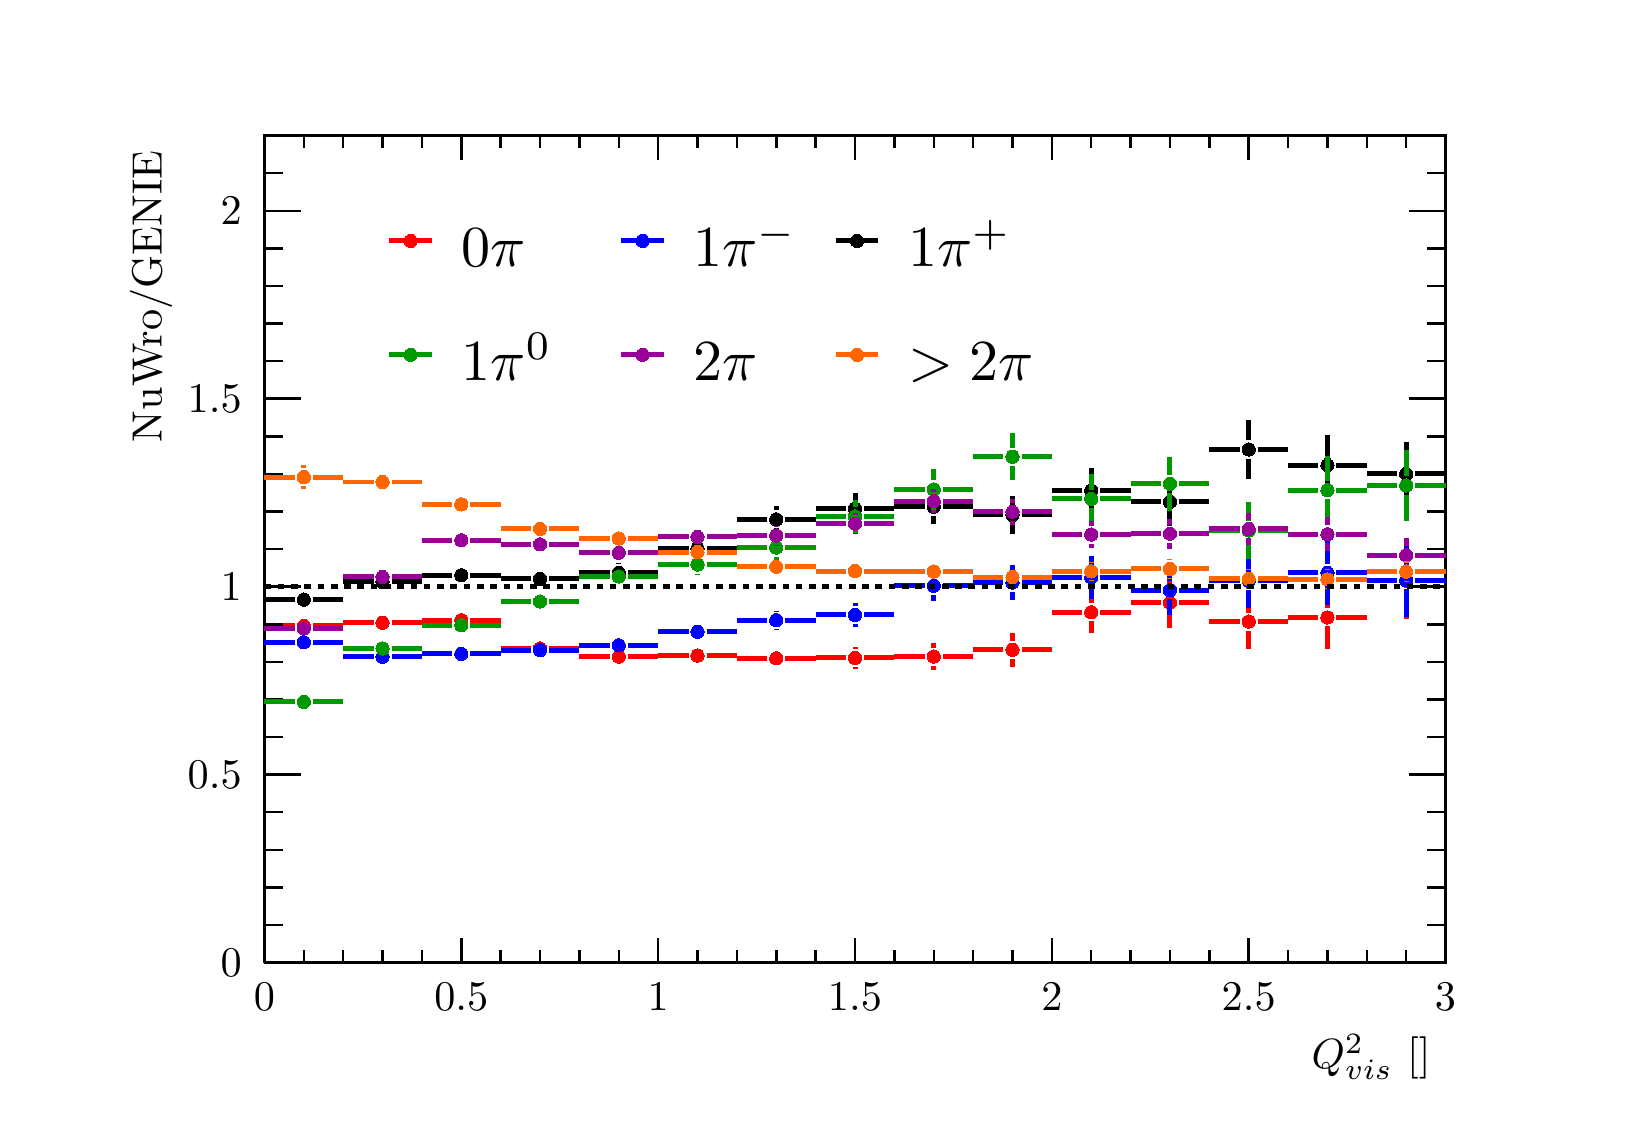
\begin{tikzpicture}
\pgfdeclareplotmark{cross} {
\pgfpathmoveto{\pgfpoint{-0.3\pgfplotmarksize}{\pgfplotmarksize}}
\pgfpathlineto{\pgfpoint{+0.3\pgfplotmarksize}{\pgfplotmarksize}}
\pgfpathlineto{\pgfpoint{+0.3\pgfplotmarksize}{0.3\pgfplotmarksize}}
\pgfpathlineto{\pgfpoint{+1\pgfplotmarksize}{0.3\pgfplotmarksize}}
\pgfpathlineto{\pgfpoint{+1\pgfplotmarksize}{-0.3\pgfplotmarksize}}
\pgfpathlineto{\pgfpoint{+0.3\pgfplotmarksize}{-0.3\pgfplotmarksize}}
\pgfpathlineto{\pgfpoint{+0.3\pgfplotmarksize}{-1.\pgfplotmarksize}}
\pgfpathlineto{\pgfpoint{-0.3\pgfplotmarksize}{-1.\pgfplotmarksize}}
\pgfpathlineto{\pgfpoint{-0.3\pgfplotmarksize}{-0.3\pgfplotmarksize}}
\pgfpathlineto{\pgfpoint{-1.\pgfplotmarksize}{-0.3\pgfplotmarksize}}
\pgfpathlineto{\pgfpoint{-1.\pgfplotmarksize}{0.3\pgfplotmarksize}}
\pgfpathlineto{\pgfpoint{-0.3\pgfplotmarksize}{0.3\pgfplotmarksize}}
\pgfpathclose
\pgfusepathqstroke
}
\pgfdeclareplotmark{cross*} {
\pgfpathmoveto{\pgfpoint{-0.3\pgfplotmarksize}{\pgfplotmarksize}}
\pgfpathlineto{\pgfpoint{+0.3\pgfplotmarksize}{\pgfplotmarksize}}
\pgfpathlineto{\pgfpoint{+0.3\pgfplotmarksize}{0.3\pgfplotmarksize}}
\pgfpathlineto{\pgfpoint{+1\pgfplotmarksize}{0.3\pgfplotmarksize}}
\pgfpathlineto{\pgfpoint{+1\pgfplotmarksize}{-0.3\pgfplotmarksize}}
\pgfpathlineto{\pgfpoint{+0.3\pgfplotmarksize}{-0.3\pgfplotmarksize}}
\pgfpathlineto{\pgfpoint{+0.3\pgfplotmarksize}{-1.\pgfplotmarksize}}
\pgfpathlineto{\pgfpoint{-0.3\pgfplotmarksize}{-1.\pgfplotmarksize}}
\pgfpathlineto{\pgfpoint{-0.3\pgfplotmarksize}{-0.3\pgfplotmarksize}}
\pgfpathlineto{\pgfpoint{-1.\pgfplotmarksize}{-0.3\pgfplotmarksize}}
\pgfpathlineto{\pgfpoint{-1.\pgfplotmarksize}{0.3\pgfplotmarksize}}
\pgfpathlineto{\pgfpoint{-0.3\pgfplotmarksize}{0.3\pgfplotmarksize}}
\pgfpathclose
\pgfusepathqfillstroke
}
\pgfdeclareplotmark{newstar} {
\pgfpathmoveto{\pgfqpoint{0pt}{\pgfplotmarksize}}
\pgfpathlineto{\pgfqpointpolar{44}{0.5\pgfplotmarksize}}
\pgfpathlineto{\pgfqpointpolar{18}{\pgfplotmarksize}}
\pgfpathlineto{\pgfqpointpolar{-20}{0.5\pgfplotmarksize}}
\pgfpathlineto{\pgfqpointpolar{-54}{\pgfplotmarksize}}
\pgfpathlineto{\pgfqpointpolar{-90}{0.5\pgfplotmarksize}}
\pgfpathlineto{\pgfqpointpolar{234}{\pgfplotmarksize}}
\pgfpathlineto{\pgfqpointpolar{198}{0.5\pgfplotmarksize}}
\pgfpathlineto{\pgfqpointpolar{162}{\pgfplotmarksize}}
\pgfpathlineto{\pgfqpointpolar{134}{0.5\pgfplotmarksize}}
\pgfpathclose
\pgfusepathqstroke
}
\pgfdeclareplotmark{newstar*} {
\pgfpathmoveto{\pgfqpoint{0pt}{\pgfplotmarksize}}
\pgfpathlineto{\pgfqpointpolar{44}{0.5\pgfplotmarksize}}
\pgfpathlineto{\pgfqpointpolar{18}{\pgfplotmarksize}}
\pgfpathlineto{\pgfqpointpolar{-20}{0.5\pgfplotmarksize}}
\pgfpathlineto{\pgfqpointpolar{-54}{\pgfplotmarksize}}
\pgfpathlineto{\pgfqpointpolar{-90}{0.5\pgfplotmarksize}}
\pgfpathlineto{\pgfqpointpolar{234}{\pgfplotmarksize}}
\pgfpathlineto{\pgfqpointpolar{198}{0.5\pgfplotmarksize}}
\pgfpathlineto{\pgfqpointpolar{162}{\pgfplotmarksize}}
\pgfpathlineto{\pgfqpointpolar{134}{0.5\pgfplotmarksize}}
\pgfpathclose
\pgfusepathqfillstroke
}
\definecolor{c}{rgb}{1,1,1};
\draw [color=c, fill=c] (0,0) rectangle (20,13.639);
\draw [color=c, fill=c] (3,1.77307) rectangle (18,12.2751);
\definecolor{c}{rgb}{0,0,0};
\draw [c,line width=0.9] (3,1.77307) -- (3,12.2751) -- (18,12.2751) -- (18,1.77307) -- (3,1.77307);
\definecolor{c}{rgb}{1,1,1};
\draw [color=c, fill=c] (3,1.77307) rectangle (18,12.2751);
\definecolor{c}{rgb}{0,0,0};
\draw [c,line width=0.9] (3,1.77307) -- (3,12.2751) -- (18,12.2751) -- (18,1.77307) -- (3,1.77307);
\definecolor{c}{rgb}{1,0,0};
\draw [c,line width=1.8] (3,6.04743) -- (3.38539,6.04743);
\draw [c,line width=1.8] (3.61461,6.04743) -- (4,6.04743);
\foreach \P in {(3.5,6.04743)}{\draw[mark options={color=c,fill=c},mark size=2.402402pt, line width=0.000000pt, mark=*] plot coordinates {\P};}
\draw [c,line width=1.8] (4,6.08852) -- (4.38539,6.08852);
\draw [c,line width=1.8] (4.61461,6.08852) -- (5,6.08852);
\foreach \P in {(4.5,6.08852)}{\draw[mark options={color=c,fill=c},mark size=2.402402pt, line width=0.000000pt, mark=*] plot coordinates {\P};}
\draw [c,line width=1.8] (5,6.12089) -- (5.38539,6.12089);
\draw [c,line width=1.8] (5.61461,6.12089) -- (6,6.12089);
\foreach \P in {(5.5,6.12089)}{\draw[mark options={color=c,fill=c},mark size=2.402402pt, line width=0.000000pt, mark=*] plot coordinates {\P};}
\draw [c,line width=1.8] (6,5.76282) -- (6.38539,5.76282);
\draw [c,line width=1.8] (6.61461,5.76282) -- (7,5.76282);
\foreach \P in {(6.5,5.76282)}{\draw[mark options={color=c,fill=c},mark size=2.402402pt, line width=0.000000pt, mark=*] plot coordinates {\P};}
\draw [c,line width=1.8] (7,5.65759) -- (7.38539,5.65759);
\draw [c,line width=1.8] (7.61461,5.65759) -- (8,5.65759);
\foreach \P in {(7.5,5.65759)}{\draw[mark options={color=c,fill=c},mark size=2.402402pt, line width=0.000000pt, mark=*] plot coordinates {\P};}
\draw [c,line width=1.8] (8,5.6708) -- (8.38539,5.6708);
\draw [c,line width=1.8] (8.61461,5.6708) -- (9,5.6708);
\foreach \P in {(8.5,5.6708)}{\draw[mark options={color=c,fill=c},mark size=2.402402pt, line width=0.000000pt, mark=*] plot coordinates {\P};}
\draw [c,line width=1.8] (9,5.63729) -- (9.38539,5.63729);
\draw [c,line width=1.8] (9.61461,5.63729) -- (10,5.63729);
\foreach \P in {(9.5,5.63729)}{\draw[mark options={color=c,fill=c},mark size=2.402402pt, line width=0.000000pt, mark=*] plot coordinates {\P};}
\draw [c,line width=1.8] (10.5,5.50269) -- (10.5,5.52734);
\draw [c,line width=1.8] (10.5,5.75657) -- (10.5,5.78122);
\draw [c,line width=1.8] (10,5.64196) -- (10.3854,5.64196);
\draw [c,line width=1.8] (10.6146,5.64196) -- (11,5.64196);
\foreach \P in {(10.5,5.64196)}{\draw[mark options={color=c,fill=c},mark size=2.402402pt, line width=0.000000pt, mark=*] plot coordinates {\P};}
\draw [c,line width=1.8] (11.5,5.48713) -- (11.5,5.54456);
\draw [c,line width=1.8] (11.5,5.77379) -- (11.5,5.83122);
\draw [c,line width=1.8] (11,5.65918) -- (11.3854,5.65918);
\draw [c,line width=1.8] (11.6146,5.65918) -- (12,5.65918);
\foreach \P in {(11.5,5.65918)}{\draw[mark options={color=c,fill=c},mark size=2.402402pt, line width=0.000000pt, mark=*] plot coordinates {\P};}
\draw [c,line width=1.8] (12.5,5.53191) -- (12.5,5.63008);
\draw [c,line width=1.8] (12.5,5.8593) -- (12.5,5.95747);
\draw [c,line width=1.8] (12,5.74469) -- (12.3854,5.74469);
\draw [c,line width=1.8] (12.6146,5.74469) -- (13,5.74469);
\foreach \P in {(12.5,5.74469)}{\draw[mark options={color=c,fill=c},mark size=2.402402pt, line width=0.000000pt, mark=*] plot coordinates {\P};}
\draw [c,line width=1.8] (13.5,5.95411) -- (13.5,6.10723);
\draw [c,line width=1.8] (13.5,6.33645) -- (13.5,6.48956);
\draw [c,line width=1.8] (13,6.22184) -- (13.3854,6.22184);
\draw [c,line width=1.8] (13.6146,6.22184) -- (14,6.22184);
\foreach \P in {(13.5,6.22184)}{\draw[mark options={color=c,fill=c},mark size=2.402402pt, line width=0.000000pt, mark=*] plot coordinates {\P};}
\draw [c,line width=1.8] (14.5,6.02788) -- (14.5,6.22779);
\draw [c,line width=1.8] (14.5,6.45701) -- (14.5,6.65692);
\draw [c,line width=1.8] (14,6.3424) -- (14.3854,6.3424);
\draw [c,line width=1.8] (14.6146,6.3424) -- (15,6.3424);
\foreach \P in {(14.5,6.3424)}{\draw[mark options={color=c,fill=c},mark size=2.402402pt, line width=0.000000pt, mark=*] plot coordinates {\P};}
\draw [c,line width=1.8] (15.5,5.75695) -- (15.5,5.98918);
\draw [c,line width=1.8] (15.5,6.21841) -- (15.5,6.45065);
\draw [c,line width=1.8] (15,6.1038) -- (15.3854,6.1038);
\draw [c,line width=1.8] (15.6146,6.1038) -- (16,6.1038);
\foreach \P in {(15.5,6.1038)}{\draw[mark options={color=c,fill=c},mark size=2.402402pt, line width=0.000000pt, mark=*] plot coordinates {\P};}
\draw [c,line width=1.8] (16.5,5.76141) -- (16.5,6.04106);
\draw [c,line width=1.8] (16.5,6.27029) -- (16.5,6.54995);
\draw [c,line width=1.8] (16,6.15568) -- (16.3854,6.15568);
\draw [c,line width=1.8] (16.6146,6.15568) -- (17,6.15568);
\foreach \P in {(16.5,6.15568)}{\draw[mark options={color=c,fill=c},mark size=2.402402pt, line width=0.000000pt, mark=*] plot coordinates {\P};}
\draw [c,line width=1.8] (17.5,6.13333) -- (17.5,6.50904);
\draw [c,line width=1.8] (17.5,6.73827) -- (17.5,7.11399);
\draw [c,line width=1.8] (17,6.62366) -- (17.3854,6.62366);
\draw [c,line width=1.8] (17.6146,6.62366) -- (18,6.62366);
\foreach \P in {(17.5,6.62366)}{\draw[mark options={color=c,fill=c},mark size=2.402402pt, line width=0.000000pt, mark=*] plot coordinates {\P};}
\definecolor{c}{rgb}{0,0,0};
\draw [c,line width=0.9] (3,1.77307) -- (18,1.77307);
\draw [c,line width=0.9] (3,2.07994) -- (3,1.77307);
\draw [c,line width=0.9] (3.5,1.9265) -- (3.5,1.77307);
\draw [c,line width=0.9] (4,1.9265) -- (4,1.77307);
\draw [c,line width=0.9] (4.5,1.9265) -- (4.5,1.77307);
\draw [c,line width=0.9] (5,1.9265) -- (5,1.77307);
\draw [c,line width=0.9] (5.5,2.07994) -- (5.5,1.77307);
\draw [c,line width=0.9] (6,1.9265) -- (6,1.77307);
\draw [c,line width=0.9] (6.5,1.9265) -- (6.5,1.77307);
\draw [c,line width=0.9] (7,1.9265) -- (7,1.77307);
\draw [c,line width=0.9] (7.5,1.9265) -- (7.5,1.77307);
\draw [c,line width=0.9] (8,2.07994) -- (8,1.77307);
\draw [c,line width=0.9] (8.5,1.9265) -- (8.5,1.77307);
\draw [c,line width=0.9] (9,1.9265) -- (9,1.77307);
\draw [c,line width=0.9] (9.5,1.9265) -- (9.5,1.77307);
\draw [c,line width=0.9] (10,1.9265) -- (10,1.77307);
\draw [c,line width=0.9] (10.5,2.07994) -- (10.5,1.77307);
\draw [c,line width=0.9] (11,1.9265) -- (11,1.77307);
\draw [c,line width=0.9] (11.5,1.9265) -- (11.5,1.77307);
\draw [c,line width=0.9] (12,1.9265) -- (12,1.77307);
\draw [c,line width=0.9] (12.5,1.9265) -- (12.5,1.77307);
\draw [c,line width=0.9] (13,2.07994) -- (13,1.77307);
\draw [c,line width=0.9] (13.5,1.9265) -- (13.5,1.77307);
\draw [c,line width=0.9] (14,1.9265) -- (14,1.77307);
\draw [c,line width=0.9] (14.5,1.9265) -- (14.5,1.77307);
\draw [c,line width=0.9] (15,1.9265) -- (15,1.77307);
\draw [c,line width=0.9] (15.5,2.07994) -- (15.5,1.77307);
\draw [c,line width=0.9] (16,1.9265) -- (16,1.77307);
\draw [c,line width=0.9] (16.5,1.9265) -- (16.5,1.77307);
\draw [c,line width=0.9] (17,1.9265) -- (17,1.77307);
\draw [c,line width=0.9] (17.5,1.9265) -- (17.5,1.77307);
\draw [c,line width=0.9] (18,2.07994) -- (18,1.77307);
\draw [c,line width=0.9] (18,2.07994) -- (18,1.77307);
\draw [anchor=base] (3,1.15931) node[scale=1.52731, color=c, rotate=0]{0};
\draw [anchor=base] (5.5,1.15931) node[scale=1.52731, color=c, rotate=0]{0.5};
\draw [anchor=base] (8,1.15931) node[scale=1.52731, color=c, rotate=0]{1};
\draw [anchor=base] (10.5,1.15931) node[scale=1.52731, color=c, rotate=0]{1.5};
\draw [anchor=base] (13,1.15931) node[scale=1.52731, color=c, rotate=0]{2};
\draw [anchor=base] (15.5,1.15931) node[scale=1.52731, color=c, rotate=0]{2.5};
\draw [anchor=base] (18,1.15931) node[scale=1.52731, color=c, rotate=0]{3};
\draw [anchor= east] (18,0.572837) node[scale=1.52731, color=c, rotate=0]{ $Q^{2}_{\text{vis}}$ [\si{\giga\electronvolt\squared}] };
\draw [c,line width=0.9] (3,12.2751) -- (18,12.2751);
\draw [c,line width=0.9] (3,11.9682) -- (3,12.2751);
\draw [c,line width=0.9] (3.5,12.1216) -- (3.5,12.2751);
\draw [c,line width=0.9] (4,12.1216) -- (4,12.2751);
\draw [c,line width=0.9] (4.5,12.1216) -- (4.5,12.2751);
\draw [c,line width=0.9] (5,12.1216) -- (5,12.2751);
\draw [c,line width=0.9] (5.5,11.9682) -- (5.5,12.2751);
\draw [c,line width=0.9] (6,12.1216) -- (6,12.2751);
\draw [c,line width=0.9] (6.5,12.1216) -- (6.5,12.2751);
\draw [c,line width=0.9] (7,12.1216) -- (7,12.2751);
\draw [c,line width=0.9] (7.5,12.1216) -- (7.5,12.2751);
\draw [c,line width=0.9] (8,11.9682) -- (8,12.2751);
\draw [c,line width=0.9] (8.5,12.1216) -- (8.5,12.2751);
\draw [c,line width=0.9] (9,12.1216) -- (9,12.2751);
\draw [c,line width=0.9] (9.5,12.1216) -- (9.5,12.2751);
\draw [c,line width=0.9] (10,12.1216) -- (10,12.2751);
\draw [c,line width=0.9] (10.5,11.9682) -- (10.5,12.2751);
\draw [c,line width=0.9] (11,12.1216) -- (11,12.2751);
\draw [c,line width=0.9] (11.5,12.1216) -- (11.5,12.2751);
\draw [c,line width=0.9] (12,12.1216) -- (12,12.2751);
\draw [c,line width=0.9] (12.5,12.1216) -- (12.5,12.2751);
\draw [c,line width=0.9] (13,11.9682) -- (13,12.2751);
\draw [c,line width=0.9] (13.5,12.1216) -- (13.5,12.2751);
\draw [c,line width=0.9] (14,12.1216) -- (14,12.2751);
\draw [c,line width=0.9] (14.5,12.1216) -- (14.5,12.2751);
\draw [c,line width=0.9] (15,12.1216) -- (15,12.2751);
\draw [c,line width=0.9] (15.5,11.9682) -- (15.5,12.2751);
\draw [c,line width=0.9] (16,12.1216) -- (16,12.2751);
\draw [c,line width=0.9] (16.5,12.1216) -- (16.5,12.2751);
\draw [c,line width=0.9] (17,12.1216) -- (17,12.2751);
\draw [c,line width=0.9] (17.5,12.1216) -- (17.5,12.2751);
\draw [c,line width=0.9] (18,11.9682) -- (18,12.2751);
\draw [c,line width=0.9] (18,11.9682) -- (18,12.2751);
\draw [c,line width=0.9] (3,1.77307) -- (3,12.2751);
\draw [c,line width=0.9] (3.462,1.77307) -- (3,1.77307);
\draw [c,line width=0.9] (3.231,2.25043) -- (3,2.25043);
\draw [c,line width=0.9] (3.231,2.72779) -- (3,2.72779);
\draw [c,line width=0.9] (3.231,3.20516) -- (3,3.20516);
\draw [c,line width=0.9] (3.231,3.68252) -- (3,3.68252);
\draw [c,line width=0.9] (3.462,4.15989) -- (3,4.15989);
\draw [c,line width=0.9] (3.231,4.63725) -- (3,4.63725);
\draw [c,line width=0.9] (3.231,5.11461) -- (3,5.11461);
\draw [c,line width=0.9] (3.231,5.59198) -- (3,5.59198);
\draw [c,line width=0.9] (3.231,6.06934) -- (3,6.06934);
\draw [c,line width=0.9] (3.462,6.5467) -- (3,6.5467);
\draw [c,line width=0.9] (3.231,7.02407) -- (3,7.02407);
\draw [c,line width=0.9] (3.231,7.50143) -- (3,7.50143);
\draw [c,line width=0.9] (3.231,7.9788) -- (3,7.9788);
\draw [c,line width=0.9] (3.231,8.45616) -- (3,8.45616);
\draw [c,line width=0.9] (3.462,8.93352) -- (3,8.93352);
\draw [c,line width=0.9] (3.231,9.41089) -- (3,9.41089);
\draw [c,line width=0.9] (3.231,9.88825) -- (3,9.88825);
\draw [c,line width=0.9] (3.231,10.3656) -- (3,10.3656);
\draw [c,line width=0.9] (3.231,10.843) -- (3,10.843);
\draw [c,line width=0.9] (3.462,11.3203) -- (3,11.3203);
\draw [c,line width=0.9] (3.462,11.3203) -- (3,11.3203);
\draw [c,line width=0.9] (3.231,11.7977) -- (3,11.7977);
\draw [c,line width=0.9] (3.231,12.2751) -- (3,12.2751);
\draw [anchor= east] (2.9,1.77307) node[scale=1.52731, color=c, rotate=0]{0};
\draw [anchor= east] (2.9,4.15989) node[scale=1.52731, color=c, rotate=0]{0.5};
\draw [anchor= east] (2.9,6.5467) node[scale=1.52731, color=c, rotate=0]{1};
\draw [anchor= east] (2.9,8.93352) node[scale=1.52731, color=c, rotate=0]{1.5};
\draw [anchor= east] (2.9,11.3203) node[scale=1.52731, color=c, rotate=0]{2};
\draw [anchor= east] (1.56,12.2751) node[scale=1.52731, color=c, rotate=90]{ NuWro/GENIE};
\draw [c,line width=0.9] (18,1.77307) -- (18,12.2751);
\draw [c,line width=0.9] (17.538,1.77307) -- (18,1.77307);
\draw [c,line width=0.9] (17.769,2.25043) -- (18,2.25043);
\draw [c,line width=0.9] (17.769,2.72779) -- (18,2.72779);
\draw [c,line width=0.9] (17.769,3.20516) -- (18,3.20516);
\draw [c,line width=0.9] (17.769,3.68252) -- (18,3.68252);
\draw [c,line width=0.9] (17.538,4.15989) -- (18,4.15989);
\draw [c,line width=0.9] (17.769,4.63725) -- (18,4.63725);
\draw [c,line width=0.9] (17.769,5.11461) -- (18,5.11461);
\draw [c,line width=0.9] (17.769,5.59198) -- (18,5.59198);
\draw [c,line width=0.9] (17.769,6.06934) -- (18,6.06934);
\draw [c,line width=0.9] (17.538,6.5467) -- (18,6.5467);
\draw [c,line width=0.9] (17.769,7.02407) -- (18,7.02407);
\draw [c,line width=0.9] (17.769,7.50143) -- (18,7.50143);
\draw [c,line width=0.9] (17.769,7.9788) -- (18,7.9788);
\draw [c,line width=0.9] (17.769,8.45616) -- (18,8.45616);
\draw [c,line width=0.9] (17.538,8.93352) -- (18,8.93352);
\draw [c,line width=0.9] (17.769,9.41089) -- (18,9.41089);
\draw [c,line width=0.9] (17.769,9.88825) -- (18,9.88825);
\draw [c,line width=0.9] (17.769,10.3656) -- (18,10.3656);
\draw [c,line width=0.9] (17.769,10.843) -- (18,10.843);
\draw [c,line width=0.9] (17.538,11.3203) -- (18,11.3203);
\draw [c,line width=0.9] (17.538,11.3203) -- (18,11.3203);
\draw [c,line width=0.9] (17.769,11.7977) -- (18,11.7977);
\draw [c,line width=0.9] (17.769,12.2751) -- (18,12.2751);
\definecolor{c}{rgb}{0,0,1};
\draw [c,line width=1.8] (3,5.8411) -- (3.38539,5.8411);
\draw [c,line width=1.8] (3.61461,5.8411) -- (4,5.8411);
\foreach \P in {(3.5,5.8411)}{\draw[mark options={color=c,fill=c},mark size=2.402402pt, line width=0.000000pt, mark=*] plot coordinates {\P};}
\draw [c,line width=1.8] (4,5.65657) -- (4.38539,5.65657);
\draw [c,line width=1.8] (4.61461,5.65657) -- (5,5.65657);
\foreach \P in {(4.5,5.65657)}{\draw[mark options={color=c,fill=c},mark size=2.402402pt, line width=0.000000pt, mark=*] plot coordinates {\P};}
\draw [c,line width=1.8] (5,5.69388) -- (5.38539,5.69388);
\draw [c,line width=1.8] (5.61461,5.69388) -- (6,5.69388);
\foreach \P in {(5.5,5.69388)}{\draw[mark options={color=c,fill=c},mark size=2.402402pt, line width=0.000000pt, mark=*] plot coordinates {\P};}
\draw [c,line width=1.8] (6,5.74041) -- (6.38539,5.74041);
\draw [c,line width=1.8] (6.61461,5.74041) -- (7,5.74041);
\foreach \P in {(6.5,5.74041)}{\draw[mark options={color=c,fill=c},mark size=2.402402pt, line width=0.000000pt, mark=*] plot coordinates {\P};}
\draw [c,line width=1.8] (7,5.80259) -- (7.38539,5.80259);
\draw [c,line width=1.8] (7.61461,5.80259) -- (8,5.80259);
\foreach \P in {(7.5,5.80259)}{\draw[mark options={color=c,fill=c},mark size=2.402402pt, line width=0.000000pt, mark=*] plot coordinates {\P};}
\draw [c,line width=1.8] (8,5.97399) -- (8.38539,5.97399);
\draw [c,line width=1.8] (8.61461,5.97399) -- (9,5.97399);
\foreach \P in {(8.5,5.97399)}{\draw[mark options={color=c,fill=c},mark size=2.402402pt, line width=0.000000pt, mark=*] plot coordinates {\P};}
\draw [c,line width=1.8] (9.5,5.99969) -- (9.5,6.00656);
\draw [c,line width=1.8] (9.5,6.23578) -- (9.5,6.24265);
\draw [c,line width=1.8] (9,6.12117) -- (9.38539,6.12117);
\draw [c,line width=1.8] (9.61461,6.12117) -- (10,6.12117);
\foreach \P in {(9.5,6.12117)}{\draw[mark options={color=c,fill=c},mark size=2.402402pt, line width=0.000000pt, mark=*] plot coordinates {\P};}
\draw [c,line width=1.8] (10.5,6.0396) -- (10.5,6.07429);
\draw [c,line width=1.8] (10.5,6.30352) -- (10.5,6.3382);
\draw [c,line width=1.8] (10,6.1889) -- (10.3854,6.1889);
\draw [c,line width=1.8] (10.6146,6.1889) -- (11,6.1889);
\foreach \P in {(10.5,6.1889)}{\draw[mark options={color=c,fill=c},mark size=2.402402pt, line width=0.000000pt, mark=*] plot coordinates {\P};}
\draw [c,line width=1.8] (11.5,6.36671) -- (11.5,6.44376);
\draw [c,line width=1.8] (11.5,6.67299) -- (11.5,6.75003);
\draw [c,line width=1.8] (11,6.55837) -- (11.3854,6.55837);
\draw [c,line width=1.8] (11.6146,6.55837) -- (12,6.55837);
\foreach \P in {(11.5,6.55837)}{\draw[mark options={color=c,fill=c},mark size=2.402402pt, line width=0.000000pt, mark=*] plot coordinates {\P};}
\draw [c,line width=1.8] (12.5,6.3725) -- (12.5,6.48521);
\draw [c,line width=1.8] (12.5,6.71443) -- (12.5,6.82713);
\draw [c,line width=1.8] (12,6.59982) -- (12.3854,6.59982);
\draw [c,line width=1.8] (12.6146,6.59982) -- (13,6.59982);
\foreach \P in {(12.5,6.59982)}{\draw[mark options={color=c,fill=c},mark size=2.402402pt, line width=0.000000pt, mark=*] plot coordinates {\P};}
\draw [c,line width=1.8] (13.5,6.39344) -- (13.5,6.5512);
\draw [c,line width=1.8] (13.5,6.78043) -- (13.5,6.93819);
\draw [c,line width=1.8] (13,6.66581) -- (13.3854,6.66581);
\draw [c,line width=1.8] (13.6146,6.66581) -- (14,6.66581);
\foreach \P in {(13.5,6.66581)}{\draw[mark options={color=c,fill=c},mark size=2.402402pt, line width=0.000000pt, mark=*] plot coordinates {\P};}
\draw [c,line width=1.8] (14.5,6.19266) -- (14.5,6.38715);
\draw [c,line width=1.8] (14.5,6.61638) -- (14.5,6.81087);
\draw [c,line width=1.8] (14,6.50176) -- (14.3854,6.50176);
\draw [c,line width=1.8] (14.6146,6.50176) -- (15,6.50176);
\foreach \P in {(14.5,6.50176)}{\draw[mark options={color=c,fill=c},mark size=2.402402pt, line width=0.000000pt, mark=*] plot coordinates {\P};}
\draw [c,line width=1.8] (15.5,6.27302) -- (15.5,6.50785);
\draw [c,line width=1.8] (15.5,6.73708) -- (15.5,6.9719);
\draw [c,line width=1.8] (15,6.62246) -- (15.3854,6.62246);
\draw [c,line width=1.8] (15.6146,6.62246) -- (16,6.62246);
\foreach \P in {(15.5,6.62246)}{\draw[mark options={color=c,fill=c},mark size=2.402402pt, line width=0.000000pt, mark=*] plot coordinates {\P};}
\draw [c,line width=1.8] (16.5,6.30891) -- (16.5,6.60758);
\draw [c,line width=1.8] (16.5,6.83681) -- (16.5,7.13549);
\draw [c,line width=1.8] (16,6.7222) -- (16.3854,6.7222);
\draw [c,line width=1.8] (16.6146,6.7222) -- (17,6.7222);
\foreach \P in {(16.5,6.7222)}{\draw[mark options={color=c,fill=c},mark size=2.402402pt, line width=0.000000pt, mark=*] plot coordinates {\P};}
\draw [c,line width=1.8] (17.5,6.16306) -- (17.5,6.51295);
\draw [c,line width=1.8] (17.5,6.74218) -- (17.5,7.09208);
\draw [c,line width=1.8] (17,6.62757) -- (17.3854,6.62757);
\draw [c,line width=1.8] (17.6146,6.62757) -- (18,6.62757);
\foreach \P in {(17.5,6.62757)}{\draw[mark options={color=c,fill=c},mark size=2.402402pt, line width=0.000000pt, mark=*] plot coordinates {\P};}
\definecolor{c}{rgb}{0,0,0};
\draw [c,line width=1.8] (3,6.38243) -- (3.38539,6.38243);
\draw [c,line width=1.8] (3.61461,6.38243) -- (4,6.38243);
\foreach \P in {(3.5,6.38243)}{\draw[mark options={color=c,fill=c},mark size=2.402402pt, line width=0.000000pt, mark=*] plot coordinates {\P};}
\draw [c,line width=1.8] (4,6.60756) -- (4.38539,6.60756);
\draw [c,line width=1.8] (4.61461,6.60756) -- (5,6.60756);
\foreach \P in {(4.5,6.60756)}{\draw[mark options={color=c,fill=c},mark size=2.402402pt, line width=0.000000pt, mark=*] plot coordinates {\P};}
\draw [c,line width=1.8] (5,6.69119) -- (5.38539,6.69119);
\draw [c,line width=1.8] (5.61461,6.69119) -- (6,6.69119);
\foreach \P in {(5.5,6.69119)}{\draw[mark options={color=c,fill=c},mark size=2.402402pt, line width=0.000000pt, mark=*] plot coordinates {\P};}
\draw [c,line width=1.8] (6,6.64474) -- (6.38539,6.64474);
\draw [c,line width=1.8] (6.61461,6.64474) -- (7,6.64474);
\foreach \P in {(6.5,6.64474)}{\draw[mark options={color=c,fill=c},mark size=2.402402pt, line width=0.000000pt, mark=*] plot coordinates {\P};}
\draw [c,line width=1.8] (7.5,6.60047) -- (7.5,6.60934);
\draw [c,line width=1.8] (7.5,6.83857) -- (7.5,6.84744);
\draw [c,line width=1.8] (7,6.72395) -- (7.38539,6.72395);
\draw [c,line width=1.8] (7.61461,6.72395) -- (8,6.72395);
\foreach \P in {(7.5,6.72395)}{\draw[mark options={color=c,fill=c},mark size=2.402402pt, line width=0.000000pt, mark=*] plot coordinates {\P};}
\draw [c,line width=1.8] (8.5,6.88555) -- (8.5,6.91554);
\draw [c,line width=1.8] (8.5,7.14476) -- (8.5,7.17475);
\draw [c,line width=1.8] (8,7.03015) -- (8.38539,7.03015);
\draw [c,line width=1.8] (8.61461,7.03015) -- (9,7.03015);
\foreach \P in {(8.5,7.03015)}{\draw[mark options={color=c,fill=c},mark size=2.402402pt, line width=0.000000pt, mark=*] plot coordinates {\P};}
\draw [c,line width=1.8] (9.5,7.23195) -- (9.5,7.28672);
\draw [c,line width=1.8] (9.5,7.51594) -- (9.5,7.57072);
\draw [c,line width=1.8] (9,7.40133) -- (9.38539,7.40133);
\draw [c,line width=1.8] (9.61461,7.40133) -- (10,7.40133);
\foreach \P in {(9.5,7.40133)}{\draw[mark options={color=c,fill=c},mark size=2.402402pt, line width=0.000000pt, mark=*] plot coordinates {\P};}
\draw [c,line width=1.8] (10.5,7.33699) -- (10.5,7.42229);
\draw [c,line width=1.8] (10.5,7.65151) -- (10.5,7.73682);
\draw [c,line width=1.8] (10,7.5369) -- (10.3854,7.5369);
\draw [c,line width=1.8] (10.6146,7.5369) -- (11,7.5369);
\foreach \P in {(10.5,7.5369)}{\draw[mark options={color=c,fill=c},mark size=2.402402pt, line width=0.000000pt, mark=*] plot coordinates {\P};}
\draw [c,line width=1.8] (11.5,7.33972) -- (11.5,7.44719);
\draw [c,line width=1.8] (11.5,7.67642) -- (11.5,7.78389);
\draw [c,line width=1.8] (11,7.5618) -- (11.3854,7.5618);
\draw [c,line width=1.8] (11.6146,7.5618) -- (12,7.5618);
\foreach \P in {(11.5,7.5618)}{\draw[mark options={color=c,fill=c},mark size=2.402402pt, line width=0.000000pt, mark=*] plot coordinates {\P};}
\draw [c,line width=1.8] (12.5,7.21433) -- (12.5,7.34363);
\draw [c,line width=1.8] (12.5,7.57285) -- (12.5,7.70215);
\draw [c,line width=1.8] (12,7.45824) -- (12.3854,7.45824);
\draw [c,line width=1.8] (12.6146,7.45824) -- (13,7.45824);
\foreach \P in {(12.5,7.45824)}{\draw[mark options={color=c,fill=c},mark size=2.402402pt, line width=0.000000pt, mark=*] plot coordinates {\P};}
\draw [c,line width=1.8] (13.5,7.48431) -- (13.5,7.6524);
\draw [c,line width=1.8] (13.5,7.88163) -- (13.5,8.04972);
\draw [c,line width=1.8] (13,7.76701) -- (13.3854,7.76701);
\draw [c,line width=1.8] (13.6146,7.76701) -- (14,7.76701);
\foreach \P in {(13.5,7.76701)}{\draw[mark options={color=c,fill=c},mark size=2.402402pt, line width=0.000000pt, mark=*] plot coordinates {\P};}
\draw [c,line width=1.8] (14.5,7.31124) -- (14.5,7.50959);
\draw [c,line width=1.8] (14.5,7.73882) -- (14.5,7.93717);
\draw [c,line width=1.8] (14,7.62421) -- (14.3854,7.62421);
\draw [c,line width=1.8] (14.6146,7.62421) -- (15,7.62421);
\foreach \P in {(14.5,7.62421)}{\draw[mark options={color=c,fill=c},mark size=2.402402pt, line width=0.000000pt, mark=*] plot coordinates {\P};}
\draw [c,line width=1.8] (15.5,7.91638) -- (15.5,8.17441);
\draw [c,line width=1.8] (15.5,8.40363) -- (15.5,8.66166);
\draw [c,line width=1.8] (15,8.28902) -- (15.3854,8.28902);
\draw [c,line width=1.8] (15.6146,8.28902) -- (16,8.28902);
\foreach \P in {(15.5,8.28902)}{\draw[mark options={color=c,fill=c},mark size=2.402402pt, line width=0.000000pt, mark=*] plot coordinates {\P};}
\draw [c,line width=1.8] (16.5,7.70917) -- (16.5,7.97604);
\draw [c,line width=1.8] (16.5,8.20526) -- (16.5,8.47213);
\draw [c,line width=1.8] (16,8.09065) -- (16.3854,8.09065);
\draw [c,line width=1.8] (16.6146,8.09065) -- (17,8.09065);
\foreach \P in {(16.5,8.09065)}{\draw[mark options={color=c,fill=c},mark size=2.402402pt, line width=0.000000pt, mark=*] plot coordinates {\P};}
\draw [c,line width=1.8] (17.5,7.57129) -- (17.5,7.86363);
\draw [c,line width=1.8] (17.5,8.09286) -- (17.5,8.3852);
\draw [c,line width=1.8] (17,7.97824) -- (17.3854,7.97824);
\draw [c,line width=1.8] (17.6146,7.97824) -- (18,7.97824);
\foreach \P in {(17.5,7.97824)}{\draw[mark options={color=c,fill=c},mark size=2.402402pt, line width=0.000000pt, mark=*] plot coordinates {\P};}
\definecolor{c}{rgb}{0,0.6,0};
\draw [c,line width=1.8] (3,5.0845) -- (3.38539,5.0845);
\draw [c,line width=1.8] (3.61461,5.0845) -- (4,5.0845);
\foreach \P in {(3.5,5.0845)}{\draw[mark options={color=c,fill=c},mark size=2.402402pt, line width=0.000000pt, mark=*] plot coordinates {\P};}
\draw [c,line width=1.8] (4,5.76187) -- (4.38539,5.76187);
\draw [c,line width=1.8] (4.61461,5.76187) -- (5,5.76187);
\foreach \P in {(4.5,5.76187)}{\draw[mark options={color=c,fill=c},mark size=2.402402pt, line width=0.000000pt, mark=*] plot coordinates {\P};}
\draw [c,line width=1.8] (5,6.05624) -- (5.38539,6.05624);
\draw [c,line width=1.8] (5.61461,6.05624) -- (6,6.05624);
\foreach \P in {(5.5,6.05624)}{\draw[mark options={color=c,fill=c},mark size=2.402402pt, line width=0.000000pt, mark=*] plot coordinates {\P};}
\draw [c,line width=1.8] (6,6.35791) -- (6.38539,6.35791);
\draw [c,line width=1.8] (6.61461,6.35791) -- (7,6.35791);
\foreach \P in {(6.5,6.35791)}{\draw[mark options={color=c,fill=c},mark size=2.402402pt, line width=0.000000pt, mark=*] plot coordinates {\P};}
\draw [c,line width=1.8] (7,6.67594) -- (7.38539,6.67594);
\draw [c,line width=1.8] (7.61461,6.67594) -- (8,6.67594);
\foreach \P in {(7.5,6.67594)}{\draw[mark options={color=c,fill=c},mark size=2.402402pt, line width=0.000000pt, mark=*] plot coordinates {\P};}
\draw [c,line width=1.8] (8.5,6.68893) -- (8.5,6.71382);
\draw [c,line width=1.8] (8.5,6.94304) -- (8.5,6.96793);
\draw [c,line width=1.8] (8,6.82843) -- (8.38539,6.82843);
\draw [c,line width=1.8] (8.61461,6.82843) -- (9,6.82843);
\foreach \P in {(8.5,6.82843)}{\draw[mark options={color=c,fill=c},mark size=2.402402pt, line width=0.000000pt, mark=*] plot coordinates {\P};}
\draw [c,line width=1.8] (9.5,6.87207) -- (9.5,6.92823);
\draw [c,line width=1.8] (9.5,7.15746) -- (9.5,7.21361);
\draw [c,line width=1.8] (9,7.04284) -- (9.38539,7.04284);
\draw [c,line width=1.8] (9.61461,7.04284) -- (10,7.04284);
\foreach \P in {(9.5,7.04284)}{\draw[mark options={color=c,fill=c},mark size=2.402402pt, line width=0.000000pt, mark=*] plot coordinates {\P};}
\draw [c,line width=1.8] (10.5,7.22658) -- (10.5,7.32438);
\draw [c,line width=1.8] (10.5,7.55361) -- (10.5,7.65141);
\draw [c,line width=1.8] (10,7.439) -- (10.3854,7.439);
\draw [c,line width=1.8] (10.6146,7.439) -- (11,7.439);
\foreach \P in {(10.5,7.439)}{\draw[mark options={color=c,fill=c},mark size=2.402402pt, line width=0.000000pt, mark=*] plot coordinates {\P};}
\draw [c,line width=1.8] (11.5,7.52671) -- (11.5,7.66743);
\draw [c,line width=1.8] (11.5,7.89666) -- (11.5,8.03737);
\draw [c,line width=1.8] (11,7.78204) -- (11.3854,7.78204);
\draw [c,line width=1.8] (11.6146,7.78204) -- (12,7.78204);
\foreach \P in {(11.5,7.78204)}{\draw[mark options={color=c,fill=c},mark size=2.402402pt, line width=0.000000pt, mark=*] plot coordinates {\P};}
\draw [c,line width=1.8] (12.5,7.89831) -- (12.5,8.08322);
\draw [c,line width=1.8] (12.5,8.31245) -- (12.5,8.49736);
\draw [c,line width=1.8] (12,8.19783) -- (12.3854,8.19783);
\draw [c,line width=1.8] (12.6146,8.19783) -- (13,8.19783);
\foreach \P in {(12.5,8.19783)}{\draw[mark options={color=c,fill=c},mark size=2.402402pt, line width=0.000000pt, mark=*] plot coordinates {\P};}
\draw [c,line width=1.8] (13.5,7.34692) -- (13.5,7.54667);
\draw [c,line width=1.8] (13.5,7.7759) -- (13.5,7.97565);
\draw [c,line width=1.8] (13,7.66128) -- (13.3854,7.66128);
\draw [c,line width=1.8] (13.6146,7.66128) -- (14,7.66128);
\foreach \P in {(13.5,7.66128)}{\draw[mark options={color=c,fill=c},mark size=2.402402pt, line width=0.000000pt, mark=*] plot coordinates {\P};}
\draw [c,line width=1.8] (14.5,7.51028) -- (14.5,7.73894);
\draw [c,line width=1.8] (14.5,7.96817) -- (14.5,8.19684);
\draw [c,line width=1.8] (14,7.85356) -- (14.3854,7.85356);
\draw [c,line width=1.8] (14.6146,7.85356) -- (15,7.85356);
\foreach \P in {(14.5,7.85356)}{\draw[mark options={color=c,fill=c},mark size=2.402402pt, line width=0.000000pt, mark=*] plot coordinates {\P};}
\draw [c,line width=1.8] (15.5,6.89466) -- (15.5,7.14606);
\draw [c,line width=1.8] (15.5,7.37529) -- (15.5,7.62669);
\draw [c,line width=1.8] (15,7.26068) -- (15.3854,7.26068);
\draw [c,line width=1.8] (15.6146,7.26068) -- (16,7.26068);
\foreach \P in {(15.5,7.26068)}{\draw[mark options={color=c,fill=c},mark size=2.402402pt, line width=0.000000pt, mark=*] plot coordinates {\P};}
\draw [c,line width=1.8] (16.5,7.34328) -- (16.5,7.65794);
\draw [c,line width=1.8] (16.5,7.88716) -- (16.5,8.20182);
\draw [c,line width=1.8] (16,7.77255) -- (16.3854,7.77255);
\draw [c,line width=1.8] (16.6146,7.77255) -- (17,7.77255);
\foreach \P in {(16.5,7.77255)}{\draw[mark options={color=c,fill=c},mark size=2.402402pt, line width=0.000000pt, mark=*] plot coordinates {\P};}
\draw [c,line width=1.8] (17.5,7.37887) -- (17.5,7.71679);
\draw [c,line width=1.8] (17.5,7.94602) -- (17.5,8.28395);
\draw [c,line width=1.8] (17,7.83141) -- (17.3854,7.83141);
\draw [c,line width=1.8] (17.6146,7.83141) -- (18,7.83141);
\foreach \P in {(17.5,7.83141)}{\draw[mark options={color=c,fill=c},mark size=2.402402pt, line width=0.000000pt, mark=*] plot coordinates {\P};}
\definecolor{c}{rgb}{0.6,0,0.6};
\draw [c,line width=1.8] (3,6.01773) -- (3.38539,6.01773);
\draw [c,line width=1.8] (3.61461,6.01773) -- (4,6.01773);
\foreach \P in {(3.5,6.01773)}{\draw[mark options={color=c,fill=c},mark size=2.402402pt, line width=0.000000pt, mark=*] plot coordinates {\P};}
\draw [c,line width=1.8] (4,6.67018) -- (4.38539,6.67018);
\draw [c,line width=1.8] (4.61461,6.67018) -- (5,6.67018);
\foreach \P in {(4.5,6.67018)}{\draw[mark options={color=c,fill=c},mark size=2.402402pt, line width=0.000000pt, mark=*] plot coordinates {\P};}
\draw [c,line width=1.8] (5,7.13666) -- (5.38539,7.13666);
\draw [c,line width=1.8] (5.61461,7.13666) -- (6,7.13666);
\foreach \P in {(5.5,7.13666)}{\draw[mark options={color=c,fill=c},mark size=2.402402pt, line width=0.000000pt, mark=*] plot coordinates {\P};}
\draw [c,line width=1.8] (6,7.08508) -- (6.38539,7.08508);
\draw [c,line width=1.8] (6.61461,7.08508) -- (7,7.08508);
\foreach \P in {(6.5,7.08508)}{\draw[mark options={color=c,fill=c},mark size=2.402402pt, line width=0.000000pt, mark=*] plot coordinates {\P};}
\draw [c,line width=1.8] (7,6.97753) -- (7.38539,6.97753);
\draw [c,line width=1.8] (7.61461,6.97753) -- (8,6.97753);
\foreach \P in {(7.5,6.97753)}{\draw[mark options={color=c,fill=c},mark size=2.402402pt, line width=0.000000pt, mark=*] plot coordinates {\P};}
\draw [c,line width=1.8] (8,7.17875) -- (8.38539,7.17875);
\draw [c,line width=1.8] (8.61461,7.17875) -- (9,7.17875);
\foreach \P in {(8.5,7.17875)}{\draw[mark options={color=c,fill=c},mark size=2.402402pt, line width=0.000000pt, mark=*] plot coordinates {\P};}
\draw [c,line width=1.8] (9.5,7.07924) -- (9.5,7.08128);
\draw [c,line width=1.8] (9.5,7.3105) -- (9.5,7.31254);
\draw [c,line width=1.8] (9,7.19589) -- (9.38539,7.19589);
\draw [c,line width=1.8] (9.61461,7.19589) -- (10,7.19589);
\foreach \P in {(9.5,7.19589)}{\draw[mark options={color=c,fill=c},mark size=2.402402pt, line width=0.000000pt, mark=*] plot coordinates {\P};}
\draw [c,line width=1.8] (10.5,7.21138) -- (10.5,7.23198);
\draw [c,line width=1.8] (10.5,7.46121) -- (10.5,7.48181);
\draw [c,line width=1.8] (10,7.34659) -- (10.3854,7.34659);
\draw [c,line width=1.8] (10.6146,7.34659) -- (11,7.34659);
\foreach \P in {(10.5,7.34659)}{\draw[mark options={color=c,fill=c},mark size=2.402402pt, line width=0.000000pt, mark=*] plot coordinates {\P};}
\draw [c,line width=1.8] (11.5,7.48113) -- (11.5,7.51879);
\draw [c,line width=1.8] (11.5,7.74801) -- (11.5,7.78568);
\draw [c,line width=1.8] (11,7.6334) -- (11.3854,7.6334);
\draw [c,line width=1.8] (11.6146,7.6334) -- (12,7.6334);
\foreach \P in {(11.5,7.6334)}{\draw[mark options={color=c,fill=c},mark size=2.402402pt, line width=0.000000pt, mark=*] plot coordinates {\P};}
\draw [c,line width=1.8] (12.5,7.33162) -- (12.5,7.38234);
\draw [c,line width=1.8] (12.5,7.61157) -- (12.5,7.66228);
\draw [c,line width=1.8] (12,7.49695) -- (12.3854,7.49695);
\draw [c,line width=1.8] (12.6146,7.49695) -- (13,7.49695);
\foreach \P in {(12.5,7.49695)}{\draw[mark options={color=c,fill=c},mark size=2.402402pt, line width=0.000000pt, mark=*] plot coordinates {\P};}
\draw [c,line width=1.8] (13.5,7.03552) -- (13.5,7.09412);
\draw [c,line width=1.8] (13.5,7.32335) -- (13.5,7.38194);
\draw [c,line width=1.8] (13,7.20873) -- (13.3854,7.20873);
\draw [c,line width=1.8] (13.6146,7.20873) -- (14,7.20873);
\foreach \P in {(13.5,7.20873)}{\draw[mark options={color=c,fill=c},mark size=2.402402pt, line width=0.000000pt, mark=*] plot coordinates {\P};}
\draw [c,line width=1.8] (14.5,7.02919) -- (14.5,7.10444);
\draw [c,line width=1.8] (14.5,7.33367) -- (14.5,7.40893);
\draw [c,line width=1.8] (14,7.21906) -- (14.3854,7.21906);
\draw [c,line width=1.8] (14.6146,7.21906) -- (15,7.21906);
\foreach \P in {(14.5,7.21906)}{\draw[mark options={color=c,fill=c},mark size=2.402402pt, line width=0.000000pt, mark=*] plot coordinates {\P};}
\draw [c,line width=1.8] (15.5,7.07526) -- (15.5,7.16585);
\draw [c,line width=1.8] (15.5,7.39508) -- (15.5,7.48567);
\draw [c,line width=1.8] (15,7.28047) -- (15.3854,7.28047);
\draw [c,line width=1.8] (15.6146,7.28047) -- (16,7.28047);
\foreach \P in {(15.5,7.28047)}{\draw[mark options={color=c,fill=c},mark size=2.402402pt, line width=0.000000pt, mark=*] plot coordinates {\P};}
\draw [c,line width=1.8] (16.5,6.99694) -- (16.5,7.09698);
\draw [c,line width=1.8] (16.5,7.3262) -- (16.5,7.42624);
\draw [c,line width=1.8] (16,7.21159) -- (16.3854,7.21159);
\draw [c,line width=1.8] (16.6146,7.21159) -- (17,7.21159);
\foreach \P in {(16.5,7.21159)}{\draw[mark options={color=c,fill=c},mark size=2.402402pt, line width=0.000000pt, mark=*] plot coordinates {\P};}
\draw [c,line width=1.8] (17.5,6.72299) -- (17.5,6.83154);
\draw [c,line width=1.8] (17.5,7.06077) -- (17.5,7.16932);
\draw [c,line width=1.8] (17,6.94615) -- (17.3854,6.94615);
\draw [c,line width=1.8] (17.6146,6.94615) -- (18,6.94615);
\foreach \P in {(17.5,6.94615)}{\draw[mark options={color=c,fill=c},mark size=2.402402pt, line width=0.000000pt, mark=*] plot coordinates {\P};}
\definecolor{c}{rgb}{1,0.4,0};
\draw [c,line width=1.8] (3.5,7.78749) -- (3.5,7.82423);
\draw [c,line width=1.8] (3.5,8.05345) -- (3.5,8.09019);
\draw [c,line width=1.8] (3,7.93884) -- (3.38539,7.93884);
\draw [c,line width=1.8] (3.61461,7.93884) -- (4,7.93884);
\foreach \P in {(3.5,7.93884)}{\draw[mark options={color=c,fill=c},mark size=2.402402pt, line width=0.000000pt, mark=*] plot coordinates {\P};}
\draw [c,line width=1.8] (4,7.87607) -- (4.38539,7.87607);
\draw [c,line width=1.8] (4.61461,7.87607) -- (5,7.87607);
\foreach \P in {(4.5,7.87607)}{\draw[mark options={color=c,fill=c},mark size=2.402402pt, line width=0.000000pt, mark=*] plot coordinates {\P};}
\draw [c,line width=1.8] (5,7.59204) -- (5.38539,7.59204);
\draw [c,line width=1.8] (5.61461,7.59204) -- (6,7.59204);
\foreach \P in {(5.5,7.59204)}{\draw[mark options={color=c,fill=c},mark size=2.402402pt, line width=0.000000pt, mark=*] plot coordinates {\P};}
\draw [c,line width=1.8] (6,7.28163) -- (6.38539,7.28163);
\draw [c,line width=1.8] (6.61461,7.28163) -- (7,7.28163);
\foreach \P in {(6.5,7.28163)}{\draw[mark options={color=c,fill=c},mark size=2.402402pt, line width=0.000000pt, mark=*] plot coordinates {\P};}
\draw [c,line width=1.8] (7,7.15891) -- (7.38539,7.15891);
\draw [c,line width=1.8] (7.61461,7.15891) -- (8,7.15891);
\foreach \P in {(7.5,7.15891)}{\draw[mark options={color=c,fill=c},mark size=2.402402pt, line width=0.000000pt, mark=*] plot coordinates {\P};}
\draw [c,line width=1.8] (8,6.98676) -- (8.38539,6.98676);
\draw [c,line width=1.8] (8.61461,6.98676) -- (9,6.98676);
\foreach \P in {(8.5,6.98676)}{\draw[mark options={color=c,fill=c},mark size=2.402402pt, line width=0.000000pt, mark=*] plot coordinates {\P};}
\draw [c,line width=1.8] (9,6.7994) -- (9.38539,6.7994);
\draw [c,line width=1.8] (9.61461,6.7994) -- (10,6.7994);
\foreach \P in {(9.5,6.7994)}{\draw[mark options={color=c,fill=c},mark size=2.402402pt, line width=0.000000pt, mark=*] plot coordinates {\P};}
\draw [c,line width=1.8] (10,6.74503) -- (10.3854,6.74503);
\draw [c,line width=1.8] (10.6146,6.74503) -- (11,6.74503);
\foreach \P in {(10.5,6.74503)}{\draw[mark options={color=c,fill=c},mark size=2.402402pt, line width=0.000000pt, mark=*] plot coordinates {\P};}
\draw [c,line width=1.8] (11,6.73919) -- (11.3854,6.73919);
\draw [c,line width=1.8] (11.6146,6.73919) -- (12,6.73919);
\foreach \P in {(11.5,6.73919)}{\draw[mark options={color=c,fill=c},mark size=2.402402pt, line width=0.000000pt, mark=*] plot coordinates {\P};}
\draw [c,line width=1.8] (12,6.66898) -- (12.3854,6.66898);
\draw [c,line width=1.8] (12.6146,6.66898) -- (13,6.66898);
\foreach \P in {(12.5,6.66898)}{\draw[mark options={color=c,fill=c},mark size=2.402402pt, line width=0.000000pt, mark=*] plot coordinates {\P};}
\draw [c,line width=1.8] (13.5,6.62536) -- (13.5,6.62657);
\draw [c,line width=1.8] (13.5,6.8558) -- (13.5,6.85702);
\draw [c,line width=1.8] (13,6.74119) -- (13.3854,6.74119);
\draw [c,line width=1.8] (13.6146,6.74119) -- (14,6.74119);
\foreach \P in {(13.5,6.74119)}{\draw[mark options={color=c,fill=c},mark size=2.402402pt, line width=0.000000pt, mark=*] plot coordinates {\P};}
\draw [c,line width=1.8] (14.5,6.65103) -- (14.5,6.6583);
\draw [c,line width=1.8] (14.5,6.88752) -- (14.5,6.89479);
\draw [c,line width=1.8] (14,6.77291) -- (14.3854,6.77291);
\draw [c,line width=1.8] (14.6146,6.77291) -- (15,6.77291);
\foreach \P in {(14.5,6.77291)}{\draw[mark options={color=c,fill=c},mark size=2.402402pt, line width=0.000000pt, mark=*] plot coordinates {\P};}
\draw [c,line width=1.8] (15.5,6.52271) -- (15.5,6.53011);
\draw [c,line width=1.8] (15.5,6.75934) -- (15.5,6.76674);
\draw [c,line width=1.8] (15,6.64473) -- (15.3854,6.64473);
\draw [c,line width=1.8] (15.6146,6.64473) -- (16,6.64473);
\foreach \P in {(15.5,6.64473)}{\draw[mark options={color=c,fill=c},mark size=2.402402pt, line width=0.000000pt, mark=*] plot coordinates {\P};}
\draw [c,line width=1.8] (16.5,6.51195) -- (16.5,6.52436);
\draw [c,line width=1.8] (16.5,6.75359) -- (16.5,6.766);
\draw [c,line width=1.8] (16,6.63897) -- (16.3854,6.63897);
\draw [c,line width=1.8] (16.6146,6.63897) -- (17,6.63897);
\foreach \P in {(16.5,6.63897)}{\draw[mark options={color=c,fill=c},mark size=2.402402pt, line width=0.000000pt, mark=*] plot coordinates {\P};}
\draw [c,line width=1.8] (17.5,6.60401) -- (17.5,6.62301);
\draw [c,line width=1.8] (17.5,6.85223) -- (17.5,6.87123);
\draw [c,line width=1.8] (17,6.73762) -- (17.3854,6.73762);
\draw [c,line width=1.8] (17.6146,6.73762) -- (18,6.73762);
\foreach \P in {(17.5,6.73762)}{\draw[mark options={color=c,fill=c},mark size=2.402402pt, line width=0.000000pt, mark=*] plot coordinates {\P};}
\definecolor{c}{rgb}{0,0,0};
\draw [c,dash pattern=on 2.40pt off 2.40pt ,line width=1.8] (3,6.5467) -- (18,6.5467);
\definecolor{c}{rgb}{1,1,1};
\draw [color=c, fill=c] (2,12.8206) rectangle (18,13.5708);
\definecolor{c}{rgb}{0,0,0};
%\draw (10,13.1957) node[scale=1.40004, color=c, rotate=0]{$0\pi$};
\definecolor{c}{rgb}{1,1,1};
\draw [color=c, fill=c] (4.46991,8.76791) rectangle (13.7536,11.6619);
\definecolor{c}{rgb}{0,0,0};
\draw [anchor=base west] (5.24355,10.6128) node[scale=2.10006, color=c, rotate=0]{$0\pi$};
\definecolor{c}{rgb}{1,1,1};
\draw [c, fill=c] (4.58596,10.4319) -- (5.12751,10.4319) -- (5.12751,11.4448) -- (4.58596,11.4448);
\definecolor{c}{rgb}{1,0,0};
\draw [c,line width=1.8] (4.58596,10.9384) -- (5.12751,10.9384);
\foreach \P in {(4.85673,10.9384)}{\draw[mark options={color=c,fill=c},mark size=2.402402pt, line width=0.000000pt, mark=*] plot coordinates {\P};}
\definecolor{c}{rgb}{0,0,0};
\draw [anchor=base west] (8.18957,10.6128) node[scale=2.10006, color=c, rotate=0]{$1\pi^{-}$};
\definecolor{c}{rgb}{1,1,1};
\draw [c, fill=c] (7.53198,10.4319) -- (8.07352,10.4319) -- (8.07352,11.4448) -- (7.53198,11.4448);
\definecolor{c}{rgb}{0,0,1};
\draw [c,line width=1.8] (7.53198,10.9384) -- (8.07352,10.9384);
\foreach \P in {(7.80275,10.9384)}{\draw[mark options={color=c,fill=c},mark size=2.402402pt, line width=0.000000pt, mark=*] plot coordinates {\P};}
\definecolor{c}{rgb}{0,0,0};
\draw [anchor=base west] (10.9128,10.6128) node[scale=2.10006, color=c, rotate=0]{$1\pi^{+}$};
\definecolor{c}{rgb}{1,1,1};
\draw [c, fill=c] (10.2552,10.4319) -- (10.7967,10.4319) -- (10.7967,11.4448) -- (10.2552,11.4448);
\definecolor{c}{rgb}{0,0,0};
\draw [c,line width=1.8] (10.2552,10.9384) -- (10.7967,10.9384);
\foreach \P in {(10.526,10.9384)}{\draw[mark options={color=c,fill=c},mark size=2.402402pt, line width=0.000000pt, mark=*] plot coordinates {\P};}
\draw [anchor=base west] (5.24355,9.16583) node[scale=2.10006, color=c, rotate=0]{$1\pi^{0}$};
\definecolor{c}{rgb}{1,1,1};
\draw [c, fill=c] (4.58596,8.98496) -- (5.12751,8.98496) -- (5.12751,9.99785) -- (4.58596,9.99785);
\definecolor{c}{rgb}{0,0.6,0};
\draw [c,line width=1.8] (4.58596,9.4914) -- (5.12751,9.4914);
\foreach \P in {(4.85673,9.4914)}{\draw[mark options={color=c,fill=c},mark size=2.402402pt, line width=0.000000pt, mark=*] plot coordinates {\P};}
\definecolor{c}{rgb}{0,0,0};
\draw [anchor=base west] (8.18957,9.16583) node[scale=2.10006, color=c, rotate=0]{$2\pi$};
\definecolor{c}{rgb}{1,1,1};
\draw [c, fill=c] (7.53198,8.98496) -- (8.07352,8.98496) -- (8.07352,9.99785) -- (7.53198,9.99785);
\definecolor{c}{rgb}{0.6,0,0.6};
\draw [c,line width=1.8] (7.53198,9.4914) -- (8.07352,9.4914);
\foreach \P in {(7.80275,9.4914)}{\draw[mark options={color=c,fill=c},mark size=2.402402pt, line width=0.000000pt, mark=*] plot coordinates {\P};}
\definecolor{c}{rgb}{0,0,0};
\draw [anchor=base west] (10.9128,9.16583) node[scale=2.10006, color=c, rotate=0]{$>2\pi$};
\definecolor{c}{rgb}{1,1,1};
\draw [c, fill=c] (10.2552,8.98496) -- (10.7967,8.98496) -- (10.7967,9.99785) -- (10.2552,9.99785);
\definecolor{c}{rgb}{1,0.4,0};
\draw [c,line width=1.8] (10.2552,9.4914) -- (10.7967,9.4914);
\foreach \P in {(10.526,9.4914)}{\draw[mark options={color=c,fill=c},mark size=2.402402pt, line width=0.000000pt, mark=*] plot coordinates {\P};}
\end{tikzpicture}

		\end{adjustbox}
	\end{minipage}
	\caption[Comparison of NuWro and GENIE in $Q^{2}_{\textrm{vis}}$ for RHC]{Ratio of NuWro to GENIE event rates in ND-GAr as a function of $Q^{2}_{\textrm{vis}}$ with the beam in RHC mode. Left: Reconstructed selection. Right: True selection.}
	\label{fig:Q2CompRhc}
\end{figure}

\subsection{Liquid argon}

\section{Near detector-driven reweighting}

\subsection{Choice of variables}

\begin{figure}[h]
	\begin{subfigure}[t]{.5\linewidth}
		\begin{adjustbox}{max totalsize=\linewidth, center}
			\input{files/figures/dune_ndrwt/hq0q3FhcCat7_genie}
		\end{adjustbox}
		\caption{$0\pi$ - 1 proton}
	\end{subfigure}
	\hfill
	\begin{subfigure}[t]{.5\linewidth}
		\begin{adjustbox}{max totalsize=\linewidth, center}
			\input{files/figures/dune_ndrwt/hq0q3FhcCat8_genie}
		\end{adjustbox}
		\caption{$0\pi$ - $>1$ proton}
	\end{subfigure} \\
	\begin{subfigure}[t]{.5\linewidth}
		\begin{adjustbox}{max totalsize=\linewidth, center}
			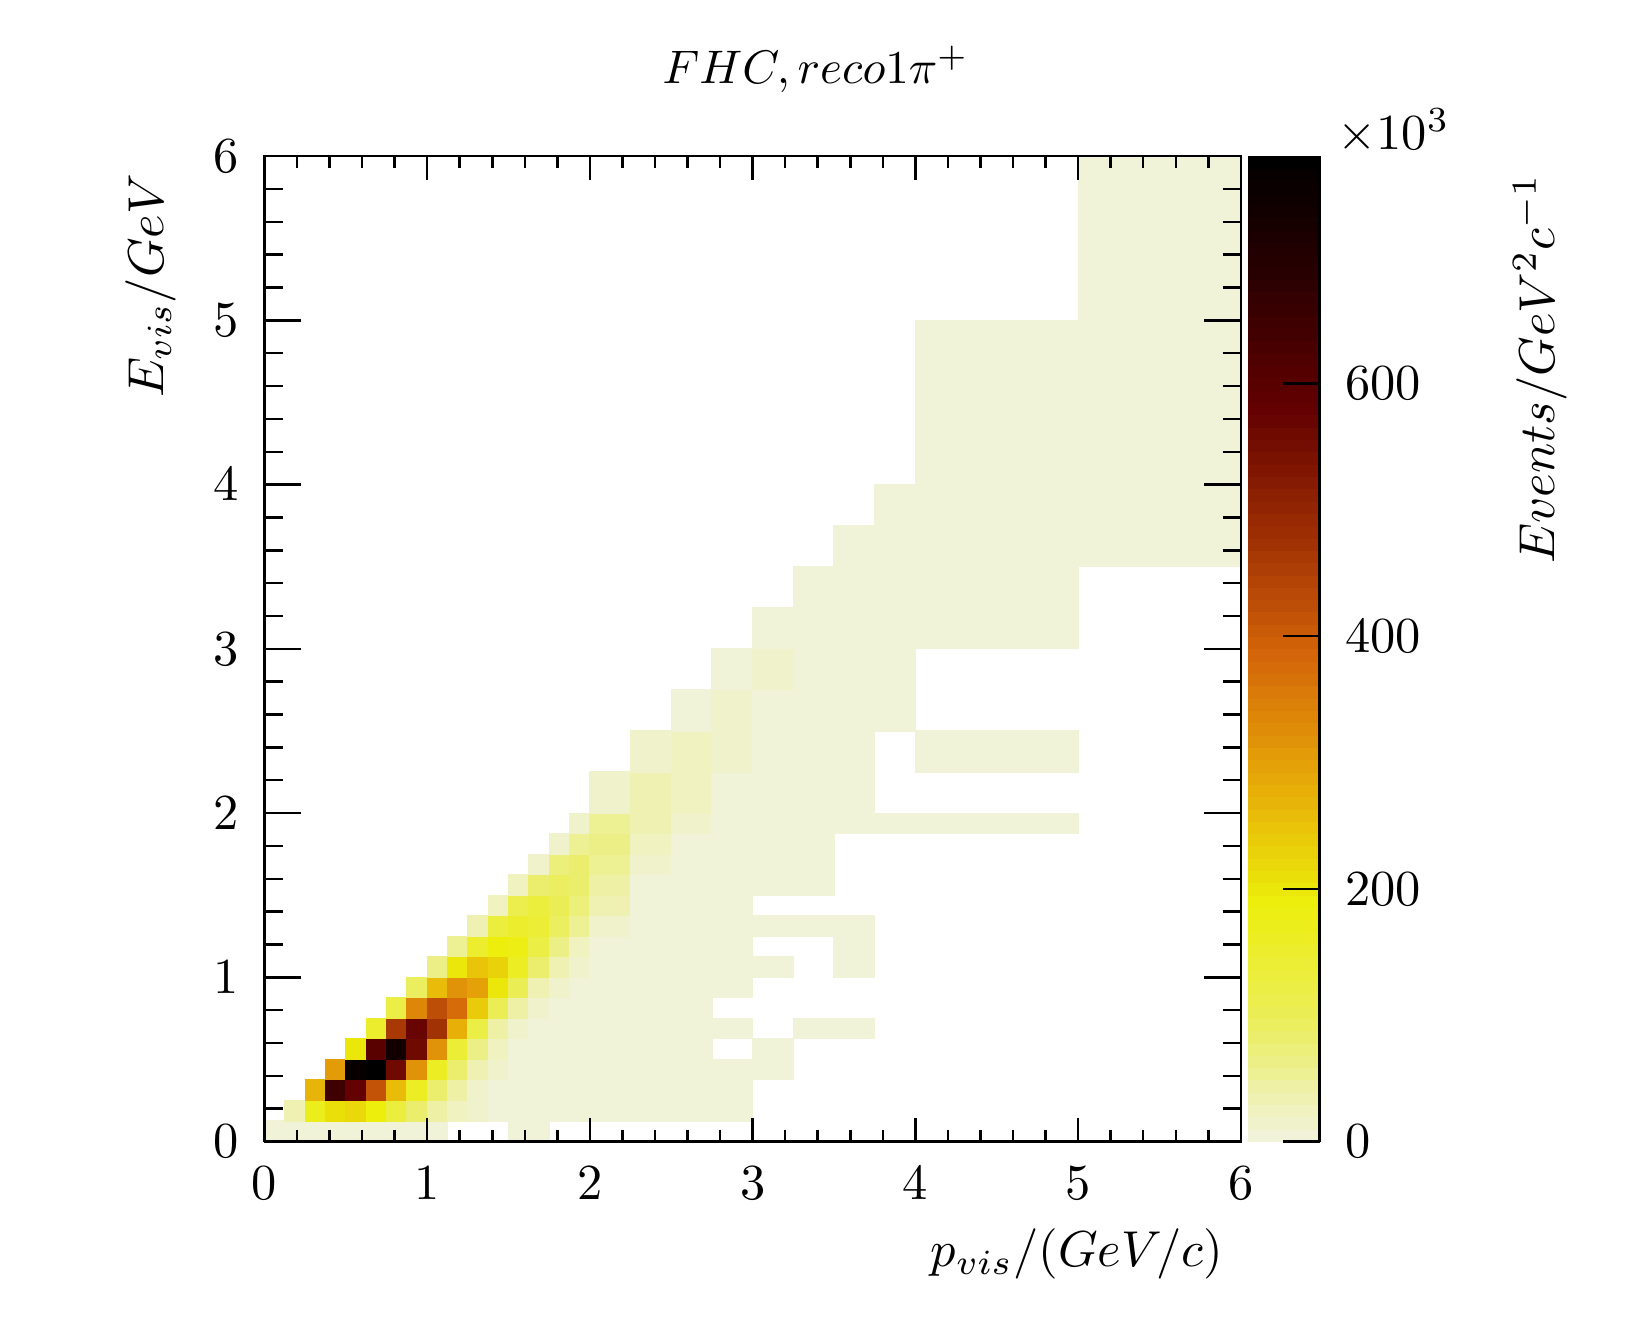
\begin{tikzpicture}
\pgfdeclareplotmark{cross} {
\pgfpathmoveto{\pgfpoint{-0.3\pgfplotmarksize}{\pgfplotmarksize}}
\pgfpathlineto{\pgfpoint{+0.3\pgfplotmarksize}{\pgfplotmarksize}}
\pgfpathlineto{\pgfpoint{+0.3\pgfplotmarksize}{0.3\pgfplotmarksize}}
\pgfpathlineto{\pgfpoint{+1\pgfplotmarksize}{0.3\pgfplotmarksize}}
\pgfpathlineto{\pgfpoint{+1\pgfplotmarksize}{-0.3\pgfplotmarksize}}
\pgfpathlineto{\pgfpoint{+0.3\pgfplotmarksize}{-0.3\pgfplotmarksize}}
\pgfpathlineto{\pgfpoint{+0.3\pgfplotmarksize}{-1.\pgfplotmarksize}}
\pgfpathlineto{\pgfpoint{-0.3\pgfplotmarksize}{-1.\pgfplotmarksize}}
\pgfpathlineto{\pgfpoint{-0.3\pgfplotmarksize}{-0.3\pgfplotmarksize}}
\pgfpathlineto{\pgfpoint{-1.\pgfplotmarksize}{-0.3\pgfplotmarksize}}
\pgfpathlineto{\pgfpoint{-1.\pgfplotmarksize}{0.3\pgfplotmarksize}}
\pgfpathlineto{\pgfpoint{-0.3\pgfplotmarksize}{0.3\pgfplotmarksize}}
\pgfpathclose
\pgfusepathqstroke
}
\pgfdeclareplotmark{cross*} {
\pgfpathmoveto{\pgfpoint{-0.3\pgfplotmarksize}{\pgfplotmarksize}}
\pgfpathlineto{\pgfpoint{+0.3\pgfplotmarksize}{\pgfplotmarksize}}
\pgfpathlineto{\pgfpoint{+0.3\pgfplotmarksize}{0.3\pgfplotmarksize}}
\pgfpathlineto{\pgfpoint{+1\pgfplotmarksize}{0.3\pgfplotmarksize}}
\pgfpathlineto{\pgfpoint{+1\pgfplotmarksize}{-0.3\pgfplotmarksize}}
\pgfpathlineto{\pgfpoint{+0.3\pgfplotmarksize}{-0.3\pgfplotmarksize}}
\pgfpathlineto{\pgfpoint{+0.3\pgfplotmarksize}{-1.\pgfplotmarksize}}
\pgfpathlineto{\pgfpoint{-0.3\pgfplotmarksize}{-1.\pgfplotmarksize}}
\pgfpathlineto{\pgfpoint{-0.3\pgfplotmarksize}{-0.3\pgfplotmarksize}}
\pgfpathlineto{\pgfpoint{-1.\pgfplotmarksize}{-0.3\pgfplotmarksize}}
\pgfpathlineto{\pgfpoint{-1.\pgfplotmarksize}{0.3\pgfplotmarksize}}
\pgfpathlineto{\pgfpoint{-0.3\pgfplotmarksize}{0.3\pgfplotmarksize}}
\pgfpathclose
\pgfusepathqfillstroke
}
\pgfdeclareplotmark{newstar} {
\pgfpathmoveto{\pgfqpoint{0pt}{\pgfplotmarksize}}
\pgfpathlineto{\pgfqpointpolar{44}{0.5\pgfplotmarksize}}
\pgfpathlineto{\pgfqpointpolar{18}{\pgfplotmarksize}}
\pgfpathlineto{\pgfqpointpolar{-20}{0.5\pgfplotmarksize}}
\pgfpathlineto{\pgfqpointpolar{-54}{\pgfplotmarksize}}
\pgfpathlineto{\pgfqpointpolar{-90}{0.5\pgfplotmarksize}}
\pgfpathlineto{\pgfqpointpolar{234}{\pgfplotmarksize}}
\pgfpathlineto{\pgfqpointpolar{198}{0.5\pgfplotmarksize}}
\pgfpathlineto{\pgfqpointpolar{162}{\pgfplotmarksize}}
\pgfpathlineto{\pgfqpointpolar{134}{0.5\pgfplotmarksize}}
\pgfpathclose
\pgfusepathqstroke
}
\pgfdeclareplotmark{newstar*} {
\pgfpathmoveto{\pgfqpoint{0pt}{\pgfplotmarksize}}
\pgfpathlineto{\pgfqpointpolar{44}{0.5\pgfplotmarksize}}
\pgfpathlineto{\pgfqpointpolar{18}{\pgfplotmarksize}}
\pgfpathlineto{\pgfqpointpolar{-20}{0.5\pgfplotmarksize}}
\pgfpathlineto{\pgfqpointpolar{-54}{\pgfplotmarksize}}
\pgfpathlineto{\pgfqpointpolar{-90}{0.5\pgfplotmarksize}}
\pgfpathlineto{\pgfqpointpolar{234}{\pgfplotmarksize}}
\pgfpathlineto{\pgfqpointpolar{198}{0.5\pgfplotmarksize}}
\pgfpathlineto{\pgfqpointpolar{162}{\pgfplotmarksize}}
\pgfpathlineto{\pgfqpointpolar{134}{0.5\pgfplotmarksize}}
\pgfpathclose
\pgfusepathqfillstroke
}
\definecolor{c}{rgb}{1,1,1};
\draw [color=c, fill=c] (0,0) rectangle (20,16.2517);
\draw [color=c, fill=c] (3,2.11272) rectangle (15.4,14.6265);
\definecolor{c}{rgb}{0,0,0};
\draw [c,line width=0.9] (3,2.11272) -- (3,14.6265) -- (15.4,14.6265) -- (15.4,2.11272) -- (3,2.11272);
\definecolor{c}{rgb}{1,1,1};
\draw [color=c, fill=c] (3,2.11272) rectangle (15.4,14.6265);
\definecolor{c}{rgb}{0,0,0};
\draw [c,line width=0.9] (3,2.11272) -- (3,14.6265) -- (15.4,14.6265) -- (15.4,2.11272) -- (3,2.11272);
\definecolor{c}{rgb}{0.945984,0.951044,0.850727};
\draw [color=c, fill=c] (3,2.11272) rectangle (3.25833,2.37343);
\draw [color=c, fill=c] (3.25833,2.11272) rectangle (3.51667,2.37343);
\draw [color=c, fill=c] (3.51667,2.11272) rectangle (3.775,2.37343);
\draw [color=c, fill=c] (3.775,2.11272) rectangle (4.03333,2.37343);
\draw [color=c, fill=c] (4.03333,2.11272) rectangle (4.29167,2.37343);
\draw [color=c, fill=c] (4.29167,2.11272) rectangle (4.55,2.37343);
\draw [color=c, fill=c] (4.55,2.11272) rectangle (4.80833,2.37343);
\draw [color=c, fill=c] (4.80833,2.11272) rectangle (5.06667,2.37343);
\draw [color=c, fill=c] (5.06667,2.11272) rectangle (5.325,2.37343);
\draw [color=c, fill=c] (6.1,2.11272) rectangle (6.35833,2.37343);
\draw [color=c, fill=c] (6.35833,2.11272) rectangle (6.61667,2.37343);
\definecolor{c}{rgb}{0.936875,0.945351,0.697027};
\draw [color=c, fill=c] (3.25833,2.37343) rectangle (3.51667,2.63413);
\definecolor{c}{rgb}{0.927206,0.933333,0.104902};
\draw [color=c, fill=c] (3.51667,2.37343) rectangle (3.775,2.63413);
\definecolor{c}{rgb}{0.923407,0.873284,0.0405637};
\draw [color=c, fill=c] (3.775,2.37343) rectangle (4.03333,2.63413);
\definecolor{c}{rgb}{0.920833,0.847549,0.0394608};
\draw [color=c, fill=c] (4.03333,2.37343) rectangle (4.29167,2.63413);
\definecolor{c}{rgb}{0.929412,0.933333,0.0431373};
\draw [color=c, fill=c] (4.29167,2.37343) rectangle (4.55,2.63413);
\definecolor{c}{rgb}{0.922426,0.933333,0.238725};
\draw [color=c, fill=c] (4.55,2.37343) rectangle (4.80833,2.63413);
\definecolor{c}{rgb}{0.920683,0.935231,0.423782};
\draw [color=c, fill=c] (4.80833,2.37343) rectangle (5.06667,2.63413);
\definecolor{c}{rgb}{0.933839,0.943453,0.645794};
\draw [color=c, fill=c] (5.06667,2.37343) rectangle (5.325,2.63413);
\definecolor{c}{rgb}{0.939911,0.947249,0.748261};
\draw [color=c, fill=c] (5.325,2.37343) rectangle (5.58333,2.63413);
\definecolor{c}{rgb}{0.942948,0.949146,0.799494};
\draw [color=c, fill=c] (5.58333,2.37343) rectangle (5.84167,2.63413);
\definecolor{c}{rgb}{0.945984,0.951044,0.850727};
\draw [color=c, fill=c] (5.84167,2.37343) rectangle (6.1,2.63413);
\draw [color=c, fill=c] (6.1,2.37343) rectangle (6.35833,2.63413);
\draw [color=c, fill=c] (6.35833,2.37343) rectangle (6.61667,2.63413);
\draw [color=c, fill=c] (6.61667,2.37343) rectangle (6.875,2.63413);
\draw [color=c, fill=c] (6.875,2.37343) rectangle (7.13333,2.63413);
\draw [color=c, fill=c] (7.13333,2.37343) rectangle (7.65,2.63413);
\draw [color=c, fill=c] (7.65,2.37343) rectangle (8.16667,2.63413);
\draw [color=c, fill=c] (8.16667,2.37343) rectangle (8.68333,2.63413);
\draw [color=c, fill=c] (8.68333,2.37343) rectangle (9.2,2.63413);
\definecolor{c}{rgb}{0.907108,0.710294,0.0335784};
\draw [color=c, fill=c] (3.51667,2.63413) rectangle (3.775,2.89484);
\definecolor{c}{rgb}{0.242647,0,0.00392157};
\draw [color=c, fill=c] (3.775,2.63413) rectangle (4.03333,2.89484);
\definecolor{c}{rgb}{0.388235,0,0.00392157};
\draw [color=c, fill=c] (4.03333,2.63413) rectangle (4.29167,2.89484);
\definecolor{c}{rgb}{0.762745,0.327451,0.0279412};
\draw [color=c, fill=c] (4.29167,2.63413) rectangle (4.55,2.89484);
\definecolor{c}{rgb}{0.909681,0.736029,0.0346814};
\draw [color=c, fill=c] (4.55,2.63413) rectangle (4.80833,2.89484);
\definecolor{c}{rgb}{0.926103,0.933333,0.135784};
\draw [color=c, fill=c] (4.80833,2.63413) rectangle (5.06667,2.89484);
\definecolor{c}{rgb}{0.920683,0.935231,0.423782};
\draw [color=c, fill=c] (5.06667,2.63413) rectangle (5.325,2.89484);
\definecolor{c}{rgb}{0.933839,0.943453,0.645794};
\draw [color=c, fill=c] (5.325,2.63413) rectangle (5.58333,2.89484);
\definecolor{c}{rgb}{0.942948,0.949146,0.799494};
\draw [color=c, fill=c] (5.58333,2.63413) rectangle (5.84167,2.89484);
\definecolor{c}{rgb}{0.945984,0.951044,0.850727};
\draw [color=c, fill=c] (5.84167,2.63413) rectangle (6.1,2.89484);
\draw [color=c, fill=c] (6.1,2.63413) rectangle (6.35833,2.89484);
\draw [color=c, fill=c] (6.35833,2.63413) rectangle (6.61667,2.89484);
\draw [color=c, fill=c] (6.61667,2.63413) rectangle (6.875,2.89484);
\draw [color=c, fill=c] (6.875,2.63413) rectangle (7.13333,2.89484);
\draw [color=c, fill=c] (7.13333,2.63413) rectangle (7.65,2.89484);
\draw [color=c, fill=c] (7.65,2.63413) rectangle (8.16667,2.89484);
\draw [color=c, fill=c] (8.16667,2.63413) rectangle (8.68333,2.89484);
\draw [color=c, fill=c] (8.68333,2.63413) rectangle (9.2,2.89484);
\definecolor{c}{rgb}{0.888726,0.609559,0.0321078};
\draw [color=c, fill=c] (3.775,2.89484) rectangle (4.03333,3.15554);
\definecolor{c}{rgb}{0.0220588,0,0.000490196};
\draw [color=c, fill=c] (4.03333,2.89484) rectangle (4.29167,3.15554);
\definecolor{c}{rgb}{0.00551471,0,0.000122549};
\draw [color=c, fill=c] (4.29167,2.89484) rectangle (4.55,3.15554);
\definecolor{c}{rgb}{0.437132,0.0386029,0.00563726};
\draw [color=c, fill=c] (4.55,2.89484) rectangle (4.80833,3.15554);
\definecolor{c}{rgb}{0.879902,0.576716,0.032598};
\draw [color=c, fill=c] (4.80833,2.89484) rectangle (5.06667,3.15554);
\definecolor{c}{rgb}{0.926103,0.933333,0.135784};
\draw [color=c, fill=c] (5.06667,2.89484) rectangle (5.325,3.15554);
\definecolor{c}{rgb}{0.920683,0.935231,0.423782};
\draw [color=c, fill=c] (5.325,2.89484) rectangle (5.58333,3.15554);
\definecolor{c}{rgb}{0.936875,0.945351,0.697027};
\draw [color=c, fill=c] (5.58333,2.89484) rectangle (5.84167,3.15554);
\definecolor{c}{rgb}{0.942948,0.949146,0.799494};
\draw [color=c, fill=c] (5.84167,2.89484) rectangle (6.1,3.15554);
\definecolor{c}{rgb}{0.945984,0.951044,0.850727};
\draw [color=c, fill=c] (6.1,2.89484) rectangle (6.35833,3.15554);
\draw [color=c, fill=c] (6.35833,2.89484) rectangle (6.61667,3.15554);
\draw [color=c, fill=c] (6.61667,2.89484) rectangle (6.875,3.15554);
\draw [color=c, fill=c] (6.875,2.89484) rectangle (7.13333,3.15554);
\draw [color=c, fill=c] (7.13333,2.89484) rectangle (7.65,3.15554);
\draw [color=c, fill=c] (7.65,2.89484) rectangle (8.16667,3.15554);
\draw [color=c, fill=c] (8.16667,2.89484) rectangle (8.68333,3.15554);
\draw [color=c, fill=c] (8.68333,2.89484) rectangle (9.2,3.15554);
\draw [color=c, fill=c] (9.2,2.89484) rectangle (9.71667,3.15554);
\definecolor{c}{rgb}{0.926838,0.907598,0.0420343};
\draw [color=c, fill=c] (4.03333,3.15554) rectangle (4.29167,3.41624);
\definecolor{c}{rgb}{0.348529,0,0.00392157};
\draw [color=c, fill=c] (4.29167,3.15554) rectangle (4.55,3.41624);
\definecolor{c}{rgb}{0.0716912,0,0.00159314};
\draw [color=c, fill=c] (4.55,3.15554) rectangle (4.80833,3.41624);
\definecolor{c}{rgb}{0.437132,0.0386029,0.00563726};
\draw [color=c, fill=c] (4.80833,3.15554) rectangle (5.06667,3.41624);
\definecolor{c}{rgb}{0.879902,0.576716,0.032598};
\draw [color=c, fill=c] (5.06667,3.15554) rectangle (5.325,3.41624);
\definecolor{c}{rgb}{0.923529,0.933333,0.207843};
\draw [color=c, fill=c] (5.325,3.15554) rectangle (5.58333,3.41624);
\definecolor{c}{rgb}{0.926755,0.939026,0.526249};
\draw [color=c, fill=c] (5.58333,3.15554) rectangle (5.84167,3.41624);
\definecolor{c}{rgb}{0.939911,0.947249,0.748261};
\draw [color=c, fill=c] (5.84167,3.15554) rectangle (6.1,3.41624);
\definecolor{c}{rgb}{0.945984,0.951044,0.850727};
\draw [color=c, fill=c] (6.1,3.15554) rectangle (6.35833,3.41624);
\draw [color=c, fill=c] (6.35833,3.15554) rectangle (6.61667,3.41624);
\draw [color=c, fill=c] (6.61667,3.15554) rectangle (6.875,3.41624);
\draw [color=c, fill=c] (6.875,3.15554) rectangle (7.13333,3.41624);
\draw [color=c, fill=c] (7.13333,3.15554) rectangle (7.65,3.41624);
\draw [color=c, fill=c] (7.65,3.15554) rectangle (8.16667,3.41624);
\draw [color=c, fill=c] (8.16667,3.15554) rectangle (8.68333,3.41624);
\draw [color=c, fill=c] (9.2,3.15554) rectangle (9.71667,3.41624);
\definecolor{c}{rgb}{0.924632,0.933333,0.176961};
\draw [color=c, fill=c] (4.29167,3.41624) rectangle (4.55,3.67695);
\definecolor{c}{rgb}{0.659804,0.22451,0.0169118};
\draw [color=c, fill=c] (4.55,3.41624) rectangle (4.80833,3.67695);
\definecolor{c}{rgb}{0.409191,0.0165441,0.00465686};
\draw [color=c, fill=c] (4.80833,3.41624) rectangle (5.06667,3.67695);
\definecolor{c}{rgb}{0.632353,0.197059,0.0139706};
\draw [color=c, fill=c] (5.06667,3.41624) rectangle (5.325,3.67695);
\definecolor{c}{rgb}{0.904534,0.684559,0.0324755};
\draw [color=c, fill=c] (5.325,3.41624) rectangle (5.58333,3.67695);
\definecolor{c}{rgb}{0.921324,0.933333,0.269608};
\draw [color=c, fill=c] (5.58333,3.41624) rectangle (5.84167,3.67695);
\definecolor{c}{rgb}{0.933839,0.943453,0.645794};
\draw [color=c, fill=c] (5.84167,3.41624) rectangle (6.1,3.67695);
\definecolor{c}{rgb}{0.942948,0.949146,0.799494};
\draw [color=c, fill=c] (6.1,3.41624) rectangle (6.35833,3.67695);
\definecolor{c}{rgb}{0.945984,0.951044,0.850727};
\draw [color=c, fill=c] (6.35833,3.41624) rectangle (6.61667,3.67695);
\draw [color=c, fill=c] (6.61667,3.41624) rectangle (6.875,3.67695);
\draw [color=c, fill=c] (6.875,3.41624) rectangle (7.13333,3.67695);
\draw [color=c, fill=c] (7.13333,3.41624) rectangle (7.65,3.67695);
\draw [color=c, fill=c] (7.65,3.41624) rectangle (8.16667,3.67695);
\draw [color=c, fill=c] (8.16667,3.41624) rectangle (8.68333,3.67695);
\draw [color=c, fill=c] (8.68333,3.41624) rectangle (9.2,3.67695);
\draw [color=c, fill=c] (9.71667,3.41624) rectangle (10.2333,3.67695);
\draw [color=c, fill=c] (10.2333,3.41624) rectangle (10.75,3.67695);
\definecolor{c}{rgb}{0.921324,0.933333,0.269608};
\draw [color=c, fill=c] (4.55,3.67695) rectangle (4.80833,3.93765);
\definecolor{c}{rgb}{0.866667,0.527451,0.0333333};
\draw [color=c, fill=c] (4.80833,3.67695) rectangle (5.06667,3.93765);
\definecolor{c}{rgb}{0.742157,0.306863,0.0257353};
\draw [color=c, fill=c] (5.06667,3.67695) rectangle (5.325,3.93765);
\definecolor{c}{rgb}{0.83799,0.420711,0.0349265};
\draw [color=c, fill=c] (5.325,3.67695) rectangle (5.58333,3.93765);
\definecolor{c}{rgb}{0.915686,0.796078,0.0372549};
\draw [color=c, fill=c] (5.58333,3.67695) rectangle (5.84167,3.93765);
\definecolor{c}{rgb}{0.919118,0.933333,0.331373};
\draw [color=c, fill=c] (5.84167,3.67695) rectangle (6.1,3.93765);
\definecolor{c}{rgb}{0.933839,0.943453,0.645794};
\draw [color=c, fill=c] (6.1,3.67695) rectangle (6.35833,3.93765);
\definecolor{c}{rgb}{0.942948,0.949146,0.799494};
\draw [color=c, fill=c] (6.35833,3.67695) rectangle (6.61667,3.93765);
\definecolor{c}{rgb}{0.945984,0.951044,0.850727};
\draw [color=c, fill=c] (6.61667,3.67695) rectangle (6.875,3.93765);
\draw [color=c, fill=c] (6.875,3.67695) rectangle (7.13333,3.93765);
\draw [color=c, fill=c] (7.13333,3.67695) rectangle (7.65,3.93765);
\draw [color=c, fill=c] (7.65,3.67695) rectangle (8.16667,3.93765);
\draw [color=c, fill=c] (8.16667,3.67695) rectangle (8.68333,3.93765);
\definecolor{c}{rgb}{0.917647,0.933333,0.372549};
\draw [color=c, fill=c] (4.80833,3.93765) rectangle (5.06667,4.19836);
\definecolor{c}{rgb}{0.909681,0.736029,0.0346814};
\draw [color=c, fill=c] (5.06667,3.93765) rectangle (5.325,4.19836);
\definecolor{c}{rgb}{0.879902,0.576716,0.032598};
\draw [color=c, fill=c] (5.325,3.93765) rectangle (5.58333,4.19836);
\definecolor{c}{rgb}{0.895343,0.634191,0.0317402};
\draw [color=c, fill=c] (5.58333,3.93765) rectangle (5.84167,4.19836);
\definecolor{c}{rgb}{0.926838,0.907598,0.0420343};
\draw [color=c, fill=c] (5.84167,3.93765) rectangle (6.1,4.19836);
\definecolor{c}{rgb}{0.919118,0.933333,0.331373};
\draw [color=c, fill=c] (6.1,3.93765) rectangle (6.35833,4.19836);
\definecolor{c}{rgb}{0.936875,0.945351,0.697027};
\draw [color=c, fill=c] (6.35833,3.93765) rectangle (6.61667,4.19836);
\definecolor{c}{rgb}{0.942948,0.949146,0.799494};
\draw [color=c, fill=c] (6.61667,3.93765) rectangle (6.875,4.19836);
\definecolor{c}{rgb}{0.945984,0.951044,0.850727};
\draw [color=c, fill=c] (6.875,3.93765) rectangle (7.13333,4.19836);
\draw [color=c, fill=c] (7.13333,3.93765) rectangle (7.65,4.19836);
\draw [color=c, fill=c] (7.65,3.93765) rectangle (8.16667,4.19836);
\draw [color=c, fill=c] (8.16667,3.93765) rectangle (8.68333,4.19836);
\draw [color=c, fill=c] (8.68333,3.93765) rectangle (9.2,4.19836);
\definecolor{c}{rgb}{0.926755,0.939026,0.526249};
\draw [color=c, fill=c] (5.06667,4.19836) rectangle (5.325,4.45906);
\definecolor{c}{rgb}{0.926838,0.907598,0.0420343};
\draw [color=c, fill=c] (5.325,4.19836) rectangle (5.58333,4.45906);
\definecolor{c}{rgb}{0.913113,0.770343,0.036152};
\draw [color=c, fill=c] (5.58333,4.19836) rectangle (5.84167,4.45906);
\definecolor{c}{rgb}{0.91826,0.821814,0.0383578};
\draw [color=c, fill=c] (5.84167,4.19836) rectangle (6.1,4.45906);
\definecolor{c}{rgb}{0.926103,0.933333,0.135784};
\draw [color=c, fill=c] (6.1,4.19836) rectangle (6.35833,4.45906);
\definecolor{c}{rgb}{0.920683,0.935231,0.423782};
\draw [color=c, fill=c] (6.35833,4.19836) rectangle (6.61667,4.45906);
\definecolor{c}{rgb}{0.936875,0.945351,0.697027};
\draw [color=c, fill=c] (6.61667,4.19836) rectangle (6.875,4.45906);
\definecolor{c}{rgb}{0.942948,0.949146,0.799494};
\draw [color=c, fill=c] (6.875,4.19836) rectangle (7.13333,4.45906);
\definecolor{c}{rgb}{0.945984,0.951044,0.850727};
\draw [color=c, fill=c] (7.13333,4.19836) rectangle (7.65,4.45906);
\draw [color=c, fill=c] (7.65,4.19836) rectangle (8.16667,4.45906);
\draw [color=c, fill=c] (8.16667,4.19836) rectangle (8.68333,4.45906);
\draw [color=c, fill=c] (8.68333,4.19836) rectangle (9.2,4.45906);
\draw [color=c, fill=c] (9.2,4.19836) rectangle (9.71667,4.45906);
\draw [color=c, fill=c] (10.2333,4.19836) rectangle (10.75,4.45906);
\definecolor{c}{rgb}{0.929791,0.940923,0.577483};
\draw [color=c, fill=c] (5.325,4.45906) rectangle (5.58333,4.71977);
\definecolor{c}{rgb}{0.924632,0.933333,0.176961};
\draw [color=c, fill=c] (5.58333,4.45906) rectangle (5.84167,4.71977);
\definecolor{c}{rgb}{0.929412,0.933333,0.0431373};
\draw [color=c, fill=c] (5.84167,4.45906) rectangle (6.1,4.71977);
\definecolor{c}{rgb}{0.928309,0.933333,0.0740196};
\draw [color=c, fill=c] (6.1,4.45906) rectangle (6.35833,4.71977);
\definecolor{c}{rgb}{0.921324,0.933333,0.269608};
\draw [color=c, fill=c] (6.35833,4.45906) rectangle (6.61667,4.71977);
\definecolor{c}{rgb}{0.926755,0.939026,0.526249};
\draw [color=c, fill=c] (6.61667,4.45906) rectangle (6.875,4.71977);
\definecolor{c}{rgb}{0.939911,0.947249,0.748261};
\draw [color=c, fill=c] (6.875,4.45906) rectangle (7.13333,4.71977);
\definecolor{c}{rgb}{0.945984,0.951044,0.850727};
\draw [color=c, fill=c] (7.13333,4.45906) rectangle (7.65,4.71977);
\draw [color=c, fill=c] (7.65,4.45906) rectangle (8.16667,4.71977);
\draw [color=c, fill=c] (8.16667,4.45906) rectangle (8.68333,4.71977);
\draw [color=c, fill=c] (8.68333,4.45906) rectangle (9.2,4.71977);
\draw [color=c, fill=c] (10.2333,4.45906) rectangle (10.75,4.71977);
\definecolor{c}{rgb}{0.936875,0.945351,0.697027};
\draw [color=c, fill=c] (5.58333,4.71977) rectangle (5.84167,4.98047);
\definecolor{c}{rgb}{0.922426,0.933333,0.238725};
\draw [color=c, fill=c] (5.84167,4.71977) rectangle (6.1,4.98047);
\definecolor{c}{rgb}{0.924632,0.933333,0.176961};
\draw [color=c, fill=c] (6.1,4.71977) rectangle (6.35833,4.98047);
\definecolor{c}{rgb}{0.923529,0.933333,0.207843};
\draw [color=c, fill=c] (6.35833,4.71977) rectangle (6.61667,4.98047);
\definecolor{c}{rgb}{0.917647,0.933333,0.372549};
\draw [color=c, fill=c] (6.61667,4.71977) rectangle (6.875,4.98047);
\definecolor{c}{rgb}{0.929791,0.940923,0.577483};
\draw [color=c, fill=c] (6.875,4.71977) rectangle (7.13333,4.98047);
\definecolor{c}{rgb}{0.942948,0.949146,0.799494};
\draw [color=c, fill=c] (7.13333,4.71977) rectangle (7.65,4.98047);
\definecolor{c}{rgb}{0.945984,0.951044,0.850727};
\draw [color=c, fill=c] (7.65,4.71977) rectangle (8.16667,4.98047);
\draw [color=c, fill=c] (8.16667,4.71977) rectangle (8.68333,4.98047);
\draw [color=c, fill=c] (8.68333,4.71977) rectangle (9.2,4.98047);
\draw [color=c, fill=c] (9.2,4.71977) rectangle (9.71667,4.98047);
\draw [color=c, fill=c] (9.71667,4.71977) rectangle (10.2333,4.98047);
\draw [color=c, fill=c] (10.2333,4.71977) rectangle (10.75,4.98047);
\definecolor{c}{rgb}{0.939911,0.947249,0.748261};
\draw [color=c, fill=c] (5.84167,4.98047) rectangle (6.1,5.24118);
\definecolor{c}{rgb}{0.920221,0.933333,0.30049};
\draw [color=c, fill=c] (6.1,4.98047) rectangle (6.35833,5.24118);
\definecolor{c}{rgb}{0.922426,0.933333,0.238725};
\draw [color=c, fill=c] (6.35833,4.98047) rectangle (6.61667,5.24118);
\definecolor{c}{rgb}{0.919118,0.933333,0.331373};
\draw [color=c, fill=c] (6.61667,4.98047) rectangle (6.875,5.24118);
\definecolor{c}{rgb}{0.923719,0.937128,0.475016};
\draw [color=c, fill=c] (6.875,4.98047) rectangle (7.13333,5.24118);
\definecolor{c}{rgb}{0.936875,0.945351,0.697027};
\draw [color=c, fill=c] (7.13333,4.98047) rectangle (7.65,5.24118);
\definecolor{c}{rgb}{0.945984,0.951044,0.850727};
\draw [color=c, fill=c] (7.65,4.98047) rectangle (8.16667,5.24118);
\draw [color=c, fill=c] (8.16667,4.98047) rectangle (8.68333,5.24118);
\draw [color=c, fill=c] (8.68333,4.98047) rectangle (9.2,5.24118);
\definecolor{c}{rgb}{0.939911,0.947249,0.748261};
\draw [color=c, fill=c] (6.1,5.24118) rectangle (6.35833,5.50188);
\definecolor{c}{rgb}{0.920683,0.935231,0.423782};
\draw [color=c, fill=c] (6.35833,5.24118) rectangle (6.61667,5.50188);
\definecolor{c}{rgb}{0.917647,0.933333,0.372549};
\draw [color=c, fill=c] (6.61667,5.24118) rectangle (6.875,5.50188);
\definecolor{c}{rgb}{0.920683,0.935231,0.423782};
\draw [color=c, fill=c] (6.875,5.24118) rectangle (7.13333,5.50188);
\definecolor{c}{rgb}{0.933839,0.943453,0.645794};
\draw [color=c, fill=c] (7.13333,5.24118) rectangle (7.65,5.50188);
\definecolor{c}{rgb}{0.945984,0.951044,0.850727};
\draw [color=c, fill=c] (7.65,5.24118) rectangle (8.16667,5.50188);
\draw [color=c, fill=c] (8.16667,5.24118) rectangle (8.68333,5.50188);
\draw [color=c, fill=c] (8.68333,5.24118) rectangle (9.2,5.50188);
\draw [color=c, fill=c] (9.2,5.24118) rectangle (9.71667,5.50188);
\draw [color=c, fill=c] (9.71667,5.24118) rectangle (10.2333,5.50188);
\definecolor{c}{rgb}{0.942948,0.949146,0.799494};
\draw [color=c, fill=c] (6.35833,5.50188) rectangle (6.61667,5.76259);
\definecolor{c}{rgb}{0.923719,0.937128,0.475016};
\draw [color=c, fill=c] (6.61667,5.50188) rectangle (6.875,5.76259);
\definecolor{c}{rgb}{0.920683,0.935231,0.423782};
\draw [color=c, fill=c] (6.875,5.50188) rectangle (7.13333,5.76259);
\definecolor{c}{rgb}{0.929791,0.940923,0.577483};
\draw [color=c, fill=c] (7.13333,5.50188) rectangle (7.65,5.76259);
\definecolor{c}{rgb}{0.942948,0.949146,0.799494};
\draw [color=c, fill=c] (7.65,5.50188) rectangle (8.16667,5.76259);
\definecolor{c}{rgb}{0.945984,0.951044,0.850727};
\draw [color=c, fill=c] (8.16667,5.50188) rectangle (8.68333,5.76259);
\draw [color=c, fill=c] (8.68333,5.50188) rectangle (9.2,5.76259);
\draw [color=c, fill=c] (9.2,5.50188) rectangle (9.71667,5.76259);
\draw [color=c, fill=c] (9.71667,5.50188) rectangle (10.2333,5.76259);
\definecolor{c}{rgb}{0.942948,0.949146,0.799494};
\draw [color=c, fill=c] (6.61667,5.76259) rectangle (6.875,6.02329);
\definecolor{c}{rgb}{0.929791,0.940923,0.577483};
\draw [color=c, fill=c] (6.875,5.76259) rectangle (7.13333,6.02329);
\definecolor{c}{rgb}{0.926755,0.939026,0.526249};
\draw [color=c, fill=c] (7.13333,5.76259) rectangle (7.65,6.02329);
\definecolor{c}{rgb}{0.939911,0.947249,0.748261};
\draw [color=c, fill=c] (7.65,5.76259) rectangle (8.16667,6.02329);
\definecolor{c}{rgb}{0.945984,0.951044,0.850727};
\draw [color=c, fill=c] (8.16667,5.76259) rectangle (8.68333,6.02329);
\draw [color=c, fill=c] (8.68333,5.76259) rectangle (9.2,6.02329);
\draw [color=c, fill=c] (9.2,5.76259) rectangle (9.71667,6.02329);
\draw [color=c, fill=c] (9.71667,5.76259) rectangle (10.2333,6.02329);
\definecolor{c}{rgb}{0.942948,0.949146,0.799494};
\draw [color=c, fill=c] (6.875,6.02329) rectangle (7.13333,6.28399);
\definecolor{c}{rgb}{0.929791,0.940923,0.577483};
\draw [color=c, fill=c] (7.13333,6.02329) rectangle (7.65,6.28399);
\definecolor{c}{rgb}{0.936875,0.945351,0.697027};
\draw [color=c, fill=c] (7.65,6.02329) rectangle (8.16667,6.28399);
\definecolor{c}{rgb}{0.942948,0.949146,0.799494};
\draw [color=c, fill=c] (8.16667,6.02329) rectangle (8.68333,6.28399);
\definecolor{c}{rgb}{0.945984,0.951044,0.850727};
\draw [color=c, fill=c] (8.68333,6.02329) rectangle (9.2,6.28399);
\draw [color=c, fill=c] (9.2,6.02329) rectangle (9.71667,6.28399);
\draw [color=c, fill=c] (9.71667,6.02329) rectangle (10.2333,6.28399);
\draw [color=c, fill=c] (10.2333,6.02329) rectangle (10.75,6.28399);
\draw [color=c, fill=c] (10.75,6.02329) rectangle (11.2667,6.28399);
\draw [color=c, fill=c] (11.2667,6.02329) rectangle (13.3333,6.28399);
\definecolor{c}{rgb}{0.942948,0.949146,0.799494};
\draw [color=c, fill=c] (7.13333,6.28399) rectangle (7.65,6.8054);
\definecolor{c}{rgb}{0.936875,0.945351,0.697027};
\draw [color=c, fill=c] (7.65,6.28399) rectangle (8.16667,6.8054);
\definecolor{c}{rgb}{0.939911,0.947249,0.748261};
\draw [color=c, fill=c] (8.16667,6.28399) rectangle (8.68333,6.8054);
\definecolor{c}{rgb}{0.945984,0.951044,0.850727};
\draw [color=c, fill=c] (8.68333,6.28399) rectangle (9.2,6.8054);
\draw [color=c, fill=c] (9.2,6.28399) rectangle (9.71667,6.8054);
\draw [color=c, fill=c] (9.71667,6.28399) rectangle (10.2333,6.8054);
\draw [color=c, fill=c] (10.2333,6.28399) rectangle (10.75,6.8054);
\definecolor{c}{rgb}{0.942948,0.949146,0.799494};
\draw [color=c, fill=c] (7.65,6.8054) rectangle (8.16667,7.32681);
\definecolor{c}{rgb}{0.939911,0.947249,0.748261};
\draw [color=c, fill=c] (8.16667,6.8054) rectangle (8.68333,7.32681);
\definecolor{c}{rgb}{0.942948,0.949146,0.799494};
\draw [color=c, fill=c] (8.68333,6.8054) rectangle (9.2,7.32681);
\definecolor{c}{rgb}{0.945984,0.951044,0.850727};
\draw [color=c, fill=c] (9.2,6.8054) rectangle (9.71667,7.32681);
\draw [color=c, fill=c] (9.71667,6.8054) rectangle (10.2333,7.32681);
\draw [color=c, fill=c] (10.2333,6.8054) rectangle (10.75,7.32681);
\draw [color=c, fill=c] (11.2667,6.8054) rectangle (13.3333,7.32681);
\draw [color=c, fill=c] (8.16667,7.32681) rectangle (8.68333,7.84822);
\definecolor{c}{rgb}{0.942948,0.949146,0.799494};
\draw [color=c, fill=c] (8.68333,7.32681) rectangle (9.2,7.84822);
\definecolor{c}{rgb}{0.945984,0.951044,0.850727};
\draw [color=c, fill=c] (9.2,7.32681) rectangle (9.71667,7.84822);
\draw [color=c, fill=c] (9.71667,7.32681) rectangle (10.2333,7.84822);
\draw [color=c, fill=c] (10.2333,7.32681) rectangle (10.75,7.84822);
\draw [color=c, fill=c] (10.75,7.32681) rectangle (11.2667,7.84822);
\draw [color=c, fill=c] (8.68333,7.84822) rectangle (9.2,8.36963);
\definecolor{c}{rgb}{0.942948,0.949146,0.799494};
\draw [color=c, fill=c] (9.2,7.84822) rectangle (9.71667,8.36963);
\definecolor{c}{rgb}{0.945984,0.951044,0.850727};
\draw [color=c, fill=c] (9.71667,7.84822) rectangle (10.2333,8.36963);
\draw [color=c, fill=c] (10.2333,7.84822) rectangle (10.75,8.36963);
\draw [color=c, fill=c] (10.75,7.84822) rectangle (11.2667,8.36963);
\draw [color=c, fill=c] (9.2,8.36963) rectangle (9.71667,8.89104);
\draw [color=c, fill=c] (9.71667,8.36963) rectangle (10.2333,8.89104);
\draw [color=c, fill=c] (10.2333,8.36963) rectangle (10.75,8.89104);
\draw [color=c, fill=c] (10.75,8.36963) rectangle (11.2667,8.89104);
\draw [color=c, fill=c] (11.2667,8.36963) rectangle (13.3333,8.89104);
\draw [color=c, fill=c] (9.71667,8.89104) rectangle (10.2333,9.41245);
\draw [color=c, fill=c] (10.2333,8.89104) rectangle (10.75,9.41245);
\draw [color=c, fill=c] (10.75,8.89104) rectangle (11.2667,9.41245);
\draw [color=c, fill=c] (11.2667,8.89104) rectangle (13.3333,9.41245);
\draw [color=c, fill=c] (10.2333,9.41245) rectangle (10.75,9.93386);
\draw [color=c, fill=c] (10.75,9.41245) rectangle (11.2667,9.93386);
\draw [color=c, fill=c] (11.2667,9.41245) rectangle (13.3333,9.93386);
\draw [color=c, fill=c] (13.3333,9.41245) rectangle (15.4,9.93386);
\draw [color=c, fill=c] (10.75,9.93386) rectangle (11.2667,10.4553);
\draw [color=c, fill=c] (11.2667,9.93386) rectangle (13.3333,10.4553);
\draw [color=c, fill=c] (13.3333,9.93386) rectangle (15.4,10.4553);
\draw [color=c, fill=c] (11.2667,10.4553) rectangle (13.3333,12.5409);
\draw [color=c, fill=c] (13.3333,10.4553) rectangle (15.4,12.5409);
\draw [color=c, fill=c] (13.3333,12.5409) rectangle (15.4,14.6265);
\definecolor{c}{rgb}{0,0,0};
\draw [c,line width=0.9] (3,2.11272) -- (15.4,2.11272);
\draw [c,line width=0.9] (3,2.415) -- (3,2.11272);
\draw [c,line width=0.9] (3.41333,2.26386) -- (3.41333,2.11272);
\draw [c,line width=0.9] (3.82667,2.26386) -- (3.82667,2.11272);
\draw [c,line width=0.9] (4.24,2.26386) -- (4.24,2.11272);
\draw [c,line width=0.9] (4.65333,2.26386) -- (4.65333,2.11272);
\draw [c,line width=0.9] (5.06667,2.415) -- (5.06667,2.11272);
\draw [c,line width=0.9] (5.48,2.26386) -- (5.48,2.11272);
\draw [c,line width=0.9] (5.89333,2.26386) -- (5.89333,2.11272);
\draw [c,line width=0.9] (6.30667,2.26386) -- (6.30667,2.11272);
\draw [c,line width=0.9] (6.72,2.26386) -- (6.72,2.11272);
\draw [c,line width=0.9] (7.13333,2.415) -- (7.13333,2.11272);
\draw [c,line width=0.9] (7.54667,2.26386) -- (7.54667,2.11272);
\draw [c,line width=0.9] (7.96,2.26386) -- (7.96,2.11272);
\draw [c,line width=0.9] (8.37333,2.26386) -- (8.37333,2.11272);
\draw [c,line width=0.9] (8.78667,2.26386) -- (8.78667,2.11272);
\draw [c,line width=0.9] (9.2,2.415) -- (9.2,2.11272);
\draw [c,line width=0.9] (9.61333,2.26386) -- (9.61333,2.11272);
\draw [c,line width=0.9] (10.0267,2.26386) -- (10.0267,2.11272);
\draw [c,line width=0.9] (10.44,2.26386) -- (10.44,2.11272);
\draw [c,line width=0.9] (10.8533,2.26386) -- (10.8533,2.11272);
\draw [c,line width=0.9] (11.2667,2.415) -- (11.2667,2.11272);
\draw [c,line width=0.9] (11.68,2.26386) -- (11.68,2.11272);
\draw [c,line width=0.9] (12.0933,2.26386) -- (12.0933,2.11272);
\draw [c,line width=0.9] (12.5067,2.26386) -- (12.5067,2.11272);
\draw [c,line width=0.9] (12.92,2.26386) -- (12.92,2.11272);
\draw [c,line width=0.9] (13.3333,2.415) -- (13.3333,2.11272);
\draw [c,line width=0.9] (13.7467,2.26386) -- (13.7467,2.11272);
\draw [c,line width=0.9] (14.16,2.26386) -- (14.16,2.11272);
\draw [c,line width=0.9] (14.5733,2.26386) -- (14.5733,2.11272);
\draw [c,line width=0.9] (14.9867,2.26386) -- (14.9867,2.11272);
\draw [c,line width=0.9] (15.4,2.415) -- (15.4,2.11272);
\draw [anchor=base] (3,1.3814) node[scale=1.82296, color=c, rotate=0]{0};
\draw [anchor=base] (5.06667,1.3814) node[scale=1.82296, color=c, rotate=0]{1};
\draw [anchor=base] (7.13333,1.3814) node[scale=1.82296, color=c, rotate=0]{2};
\draw [anchor=base] (9.2,1.3814) node[scale=1.82296, color=c, rotate=0]{3};
\draw [anchor=base] (11.2667,1.3814) node[scale=1.82296, color=c, rotate=0]{4};
\draw [anchor=base] (13.3333,1.3814) node[scale=1.82296, color=c, rotate=0]{5};
\draw [anchor=base] (15.4,1.3814) node[scale=1.82296, color=c, rotate=0]{6};
\draw [anchor= east] (15.4,0.682572) node[scale=1.82296, color=c, rotate=0]{$ p_{vis} / (GeV/c)$};
\draw [c,line width=0.9] (3,14.6265) -- (15.4,14.6265);
\draw [c,line width=0.9] (3,14.3243) -- (3,14.6265);
\draw [c,line width=0.9] (3.41333,14.4754) -- (3.41333,14.6265);
\draw [c,line width=0.9] (3.82667,14.4754) -- (3.82667,14.6265);
\draw [c,line width=0.9] (4.24,14.4754) -- (4.24,14.6265);
\draw [c,line width=0.9] (4.65333,14.4754) -- (4.65333,14.6265);
\draw [c,line width=0.9] (5.06667,14.3243) -- (5.06667,14.6265);
\draw [c,line width=0.9] (5.48,14.4754) -- (5.48,14.6265);
\draw [c,line width=0.9] (5.89333,14.4754) -- (5.89333,14.6265);
\draw [c,line width=0.9] (6.30667,14.4754) -- (6.30667,14.6265);
\draw [c,line width=0.9] (6.72,14.4754) -- (6.72,14.6265);
\draw [c,line width=0.9] (7.13333,14.3243) -- (7.13333,14.6265);
\draw [c,line width=0.9] (7.54667,14.4754) -- (7.54667,14.6265);
\draw [c,line width=0.9] (7.96,14.4754) -- (7.96,14.6265);
\draw [c,line width=0.9] (8.37333,14.4754) -- (8.37333,14.6265);
\draw [c,line width=0.9] (8.78667,14.4754) -- (8.78667,14.6265);
\draw [c,line width=0.9] (9.2,14.3243) -- (9.2,14.6265);
\draw [c,line width=0.9] (9.61333,14.4754) -- (9.61333,14.6265);
\draw [c,line width=0.9] (10.0267,14.4754) -- (10.0267,14.6265);
\draw [c,line width=0.9] (10.44,14.4754) -- (10.44,14.6265);
\draw [c,line width=0.9] (10.8533,14.4754) -- (10.8533,14.6265);
\draw [c,line width=0.9] (11.2667,14.3243) -- (11.2667,14.6265);
\draw [c,line width=0.9] (11.68,14.4754) -- (11.68,14.6265);
\draw [c,line width=0.9] (12.0933,14.4754) -- (12.0933,14.6265);
\draw [c,line width=0.9] (12.5067,14.4754) -- (12.5067,14.6265);
\draw [c,line width=0.9] (12.92,14.4754) -- (12.92,14.6265);
\draw [c,line width=0.9] (13.3333,14.3243) -- (13.3333,14.6265);
\draw [c,line width=0.9] (13.7467,14.4754) -- (13.7467,14.6265);
\draw [c,line width=0.9] (14.16,14.4754) -- (14.16,14.6265);
\draw [c,line width=0.9] (14.5733,14.4754) -- (14.5733,14.6265);
\draw [c,line width=0.9] (14.9867,14.4754) -- (14.9867,14.6265);
\draw [c,line width=0.9] (15.4,14.3243) -- (15.4,14.6265);
\draw [c,line width=0.9] (3,2.11272) -- (3,14.6265);
\draw [c,line width=0.9] (3.462,2.11272) -- (3,2.11272);
\draw [c,line width=0.9] (3.231,2.52985) -- (3,2.52985);
\draw [c,line width=0.9] (3.231,2.94698) -- (3,2.94698);
\draw [c,line width=0.9] (3.231,3.3641) -- (3,3.3641);
\draw [c,line width=0.9] (3.231,3.78123) -- (3,3.78123);
\draw [c,line width=0.9] (3.462,4.19836) -- (3,4.19836);
\draw [c,line width=0.9] (3.231,4.61549) -- (3,4.61549);
\draw [c,line width=0.9] (3.231,5.03261) -- (3,5.03261);
\draw [c,line width=0.9] (3.231,5.44974) -- (3,5.44974);
\draw [c,line width=0.9] (3.231,5.86687) -- (3,5.86687);
\draw [c,line width=0.9] (3.462,6.28399) -- (3,6.28399);
\draw [c,line width=0.9] (3.231,6.70112) -- (3,6.70112);
\draw [c,line width=0.9] (3.231,7.11825) -- (3,7.11825);
\draw [c,line width=0.9] (3.231,7.53538) -- (3,7.53538);
\draw [c,line width=0.9] (3.231,7.9525) -- (3,7.9525);
\draw [c,line width=0.9] (3.462,8.36963) -- (3,8.36963);
\draw [c,line width=0.9] (3.231,8.78676) -- (3,8.78676);
\draw [c,line width=0.9] (3.231,9.20389) -- (3,9.20389);
\draw [c,line width=0.9] (3.231,9.62101) -- (3,9.62101);
\draw [c,line width=0.9] (3.231,10.0381) -- (3,10.0381);
\draw [c,line width=0.9] (3.462,10.4553) -- (3,10.4553);
\draw [c,line width=0.9] (3.231,10.8724) -- (3,10.8724);
\draw [c,line width=0.9] (3.231,11.2895) -- (3,11.2895);
\draw [c,line width=0.9] (3.231,11.7066) -- (3,11.7066);
\draw [c,line width=0.9] (3.231,12.1238) -- (3,12.1238);
\draw [c,line width=0.9] (3.462,12.5409) -- (3,12.5409);
\draw [c,line width=0.9] (3.231,12.958) -- (3,12.958);
\draw [c,line width=0.9] (3.231,13.3752) -- (3,13.3752);
\draw [c,line width=0.9] (3.231,13.7923) -- (3,13.7923);
\draw [c,line width=0.9] (3.231,14.2094) -- (3,14.2094);
\draw [c,line width=0.9] (3.462,14.6265) -- (3,14.6265);
\draw [anchor= east] (2.9,2.11272) node[scale=1.82296, color=c, rotate=0]{0};
\draw [anchor= east] (2.9,4.19836) node[scale=1.82296, color=c, rotate=0]{1};
\draw [anchor= east] (2.9,6.28399) node[scale=1.82296, color=c, rotate=0]{2};
\draw [anchor= east] (2.9,8.36963) node[scale=1.82296, color=c, rotate=0]{3};
\draw [anchor= east] (2.9,10.4553) node[scale=1.82296, color=c, rotate=0]{4};
\draw [anchor= east] (2.9,12.5409) node[scale=1.82296, color=c, rotate=0]{5};
\draw [anchor= east] (2.9,14.6265) node[scale=1.82296, color=c, rotate=0]{6};
\draw [anchor= east] (1.56,14.6265) node[scale=1.82296, color=c, rotate=90]{$ E_{vis} / GeV$};
\draw [c,line width=0.9] (15.4,2.11272) -- (15.4,14.6265);
\draw [c,line width=0.9] (14.938,2.11272) -- (15.4,2.11272);
\draw [c,line width=0.9] (15.169,2.52985) -- (15.4,2.52985);
\draw [c,line width=0.9] (15.169,2.94698) -- (15.4,2.94698);
\draw [c,line width=0.9] (15.169,3.3641) -- (15.4,3.3641);
\draw [c,line width=0.9] (15.169,3.78123) -- (15.4,3.78123);
\draw [c,line width=0.9] (14.938,4.19836) -- (15.4,4.19836);
\draw [c,line width=0.9] (15.169,4.61549) -- (15.4,4.61549);
\draw [c,line width=0.9] (15.169,5.03261) -- (15.4,5.03261);
\draw [c,line width=0.9] (15.169,5.44974) -- (15.4,5.44974);
\draw [c,line width=0.9] (15.169,5.86687) -- (15.4,5.86687);
\draw [c,line width=0.9] (14.938,6.28399) -- (15.4,6.28399);
\draw [c,line width=0.9] (15.169,6.70112) -- (15.4,6.70112);
\draw [c,line width=0.9] (15.169,7.11825) -- (15.4,7.11825);
\draw [c,line width=0.9] (15.169,7.53538) -- (15.4,7.53538);
\draw [c,line width=0.9] (15.169,7.9525) -- (15.4,7.9525);
\draw [c,line width=0.9] (14.938,8.36963) -- (15.4,8.36963);
\draw [c,line width=0.9] (15.169,8.78676) -- (15.4,8.78676);
\draw [c,line width=0.9] (15.169,9.20389) -- (15.4,9.20389);
\draw [c,line width=0.9] (15.169,9.62101) -- (15.4,9.62101);
\draw [c,line width=0.9] (15.169,10.0381) -- (15.4,10.0381);
\draw [c,line width=0.9] (14.938,10.4553) -- (15.4,10.4553);
\draw [c,line width=0.9] (15.169,10.8724) -- (15.4,10.8724);
\draw [c,line width=0.9] (15.169,11.2895) -- (15.4,11.2895);
\draw [c,line width=0.9] (15.169,11.7066) -- (15.4,11.7066);
\draw [c,line width=0.9] (15.169,12.1238) -- (15.4,12.1238);
\draw [c,line width=0.9] (14.938,12.5409) -- (15.4,12.5409);
\draw [c,line width=0.9] (15.169,12.958) -- (15.4,12.958);
\draw [c,line width=0.9] (15.169,13.3752) -- (15.4,13.3752);
\draw [c,line width=0.9] (15.169,13.7923) -- (15.4,13.7923);
\draw [c,line width=0.9] (15.169,14.2094) -- (15.4,14.2094);
\draw [c,line width=0.9] (14.938,14.6265) -- (15.4,14.6265);
\definecolor{c}{rgb}{0.945984,0.951044,0.850727};
\draw [color=c, fill=c] (15.5,2.11272) rectangle (16.4,2.26915);
\definecolor{c}{rgb}{0.942948,0.949146,0.799494};
\draw [color=c, fill=c] (15.5,2.26915) rectangle (16.4,2.42557);
\definecolor{c}{rgb}{0.939911,0.947249,0.748261};
\draw [color=c, fill=c] (15.5,2.42557) rectangle (16.4,2.58199);
\definecolor{c}{rgb}{0.936875,0.945351,0.697027};
\draw [color=c, fill=c] (15.5,2.58199) rectangle (16.4,2.73841);
\definecolor{c}{rgb}{0.933839,0.943453,0.645794};
\draw [color=c, fill=c] (15.5,2.73841) rectangle (16.4,2.89484);
\definecolor{c}{rgb}{0.929791,0.940923,0.577483};
\draw [color=c, fill=c] (15.5,2.89484) rectangle (16.4,3.05126);
\definecolor{c}{rgb}{0.926755,0.939026,0.526249};
\draw [color=c, fill=c] (15.5,3.05126) rectangle (16.4,3.20768);
\definecolor{c}{rgb}{0.923719,0.937128,0.475016};
\draw [color=c, fill=c] (15.5,3.20768) rectangle (16.4,3.3641);
\definecolor{c}{rgb}{0.920683,0.935231,0.423782};
\draw [color=c, fill=c] (15.5,3.3641) rectangle (16.4,3.52053);
\definecolor{c}{rgb}{0.917647,0.933333,0.372549};
\draw [color=c, fill=c] (15.5,3.52053) rectangle (16.4,3.67695);
\definecolor{c}{rgb}{0.919118,0.933333,0.331373};
\draw [color=c, fill=c] (15.5,3.67695) rectangle (16.4,3.83337);
\definecolor{c}{rgb}{0.920221,0.933333,0.30049};
\draw [color=c, fill=c] (15.5,3.83337) rectangle (16.4,3.98979);
\definecolor{c}{rgb}{0.921324,0.933333,0.269608};
\draw [color=c, fill=c] (15.5,3.98979) rectangle (16.4,4.14622);
\definecolor{c}{rgb}{0.922426,0.933333,0.238725};
\draw [color=c, fill=c] (15.5,4.14622) rectangle (16.4,4.30264);
\definecolor{c}{rgb}{0.923529,0.933333,0.207843};
\draw [color=c, fill=c] (15.5,4.30264) rectangle (16.4,4.45906);
\definecolor{c}{rgb}{0.924632,0.933333,0.176961};
\draw [color=c, fill=c] (15.5,4.45906) rectangle (16.4,4.61549);
\definecolor{c}{rgb}{0.926103,0.933333,0.135784};
\draw [color=c, fill=c] (15.5,4.61549) rectangle (16.4,4.77191);
\definecolor{c}{rgb}{0.927206,0.933333,0.104902};
\draw [color=c, fill=c] (15.5,4.77191) rectangle (16.4,4.92833);
\definecolor{c}{rgb}{0.928309,0.933333,0.0740196};
\draw [color=c, fill=c] (15.5,4.92833) rectangle (16.4,5.08475);
\definecolor{c}{rgb}{0.929412,0.933333,0.0431373};
\draw [color=c, fill=c] (15.5,5.08475) rectangle (16.4,5.24118);
\definecolor{c}{rgb}{0.926838,0.907598,0.0420343};
\draw [color=c, fill=c] (15.5,5.24118) rectangle (16.4,5.3976);
\definecolor{c}{rgb}{0.923407,0.873284,0.0405637};
\draw [color=c, fill=c] (15.5,5.3976) rectangle (16.4,5.55402);
\definecolor{c}{rgb}{0.920833,0.847549,0.0394608};
\draw [color=c, fill=c] (15.5,5.55402) rectangle (16.4,5.71044);
\definecolor{c}{rgb}{0.91826,0.821814,0.0383578};
\draw [color=c, fill=c] (15.5,5.71044) rectangle (16.4,5.86687);
\definecolor{c}{rgb}{0.915686,0.796078,0.0372549};
\draw [color=c, fill=c] (15.5,5.86687) rectangle (16.4,6.02329);
\definecolor{c}{rgb}{0.913113,0.770343,0.036152};
\draw [color=c, fill=c] (15.5,6.02329) rectangle (16.4,6.17971);
\definecolor{c}{rgb}{0.909681,0.736029,0.0346814};
\draw [color=c, fill=c] (15.5,6.17971) rectangle (16.4,6.33614);
\definecolor{c}{rgb}{0.907108,0.710294,0.0335784};
\draw [color=c, fill=c] (15.5,6.33614) rectangle (16.4,6.49256);
\definecolor{c}{rgb}{0.904534,0.684559,0.0324755};
\draw [color=c, fill=c] (15.5,6.49256) rectangle (16.4,6.64898);
\definecolor{c}{rgb}{0.901961,0.658824,0.0313726};
\draw [color=c, fill=c] (15.5,6.64898) rectangle (16.4,6.8054);
\definecolor{c}{rgb}{0.895343,0.634191,0.0317402};
\draw [color=c, fill=c] (15.5,6.8054) rectangle (16.4,6.96183);
\definecolor{c}{rgb}{0.888726,0.609559,0.0321078};
\draw [color=c, fill=c] (15.5,6.96183) rectangle (16.4,7.11825);
\definecolor{c}{rgb}{0.879902,0.576716,0.032598};
\draw [color=c, fill=c] (15.5,7.11825) rectangle (16.4,7.27467);
\definecolor{c}{rgb}{0.873284,0.552083,0.0329657};
\draw [color=c, fill=c] (15.5,7.27467) rectangle (16.4,7.43109);
\definecolor{c}{rgb}{0.866667,0.527451,0.0333333};
\draw [color=c, fill=c] (15.5,7.43109) rectangle (16.4,7.58752);
\definecolor{c}{rgb}{0.860049,0.502819,0.033701};
\draw [color=c, fill=c] (15.5,7.58752) rectangle (16.4,7.74394);
\definecolor{c}{rgb}{0.853431,0.478186,0.0340686};
\draw [color=c, fill=c] (15.5,7.74394) rectangle (16.4,7.90036);
\definecolor{c}{rgb}{0.844608,0.445343,0.0345588};
\draw [color=c, fill=c] (15.5,7.90036) rectangle (16.4,8.05679);
\definecolor{c}{rgb}{0.83799,0.420711,0.0349265};
\draw [color=c, fill=c] (15.5,8.05679) rectangle (16.4,8.21321);
\definecolor{c}{rgb}{0.831373,0.396078,0.0352941};
\draw [color=c, fill=c] (15.5,8.21321) rectangle (16.4,8.36963);
\definecolor{c}{rgb}{0.810784,0.37549,0.0330882};
\draw [color=c, fill=c] (15.5,8.36963) rectangle (16.4,8.52605);
\definecolor{c}{rgb}{0.790196,0.354902,0.0308824};
\draw [color=c, fill=c] (15.5,8.52605) rectangle (16.4,8.68248);
\definecolor{c}{rgb}{0.762745,0.327451,0.0279412};
\draw [color=c, fill=c] (15.5,8.68248) rectangle (16.4,8.8389);
\definecolor{c}{rgb}{0.742157,0.306863,0.0257353};
\draw [color=c, fill=c] (15.5,8.8389) rectangle (16.4,8.99532);
\definecolor{c}{rgb}{0.721569,0.286275,0.0235294};
\draw [color=c, fill=c] (15.5,8.99532) rectangle (16.4,9.15174);
\definecolor{c}{rgb}{0.70098,0.265686,0.0213235};
\draw [color=c, fill=c] (15.5,9.15174) rectangle (16.4,9.30817);
\definecolor{c}{rgb}{0.680392,0.245098,0.0191176};
\draw [color=c, fill=c] (15.5,9.30817) rectangle (16.4,9.46459);
\definecolor{c}{rgb}{0.659804,0.22451,0.0169118};
\draw [color=c, fill=c] (15.5,9.46459) rectangle (16.4,9.62101);
\definecolor{c}{rgb}{0.632353,0.197059,0.0139706};
\draw [color=c, fill=c] (15.5,9.62101) rectangle (16.4,9.77744);
\definecolor{c}{rgb}{0.611765,0.176471,0.0117647};
\draw [color=c, fill=c] (15.5,9.77744) rectangle (16.4,9.93386);
\definecolor{c}{rgb}{0.590809,0.159926,0.0110294};
\draw [color=c, fill=c] (15.5,9.93386) rectangle (16.4,10.0903);
\definecolor{c}{rgb}{0.569853,0.143382,0.0102941};
\draw [color=c, fill=c] (15.5,10.0903) rectangle (16.4,10.2467);
\definecolor{c}{rgb}{0.548897,0.126838,0.00955882};
\draw [color=c, fill=c] (15.5,10.2467) rectangle (16.4,10.4031);
\definecolor{c}{rgb}{0.520956,0.104779,0.00857843};
\draw [color=c, fill=c] (15.5,10.4031) rectangle (16.4,10.5595);
\definecolor{c}{rgb}{0.5,0.0882353,0.00784314};
\draw [color=c, fill=c] (15.5,10.5595) rectangle (16.4,10.716);
\definecolor{c}{rgb}{0.479044,0.0716912,0.00710784};
\draw [color=c, fill=c] (15.5,10.716) rectangle (16.4,10.8724);
\definecolor{c}{rgb}{0.458088,0.0551471,0.00637255};
\draw [color=c, fill=c] (15.5,10.8724) rectangle (16.4,11.0288);
\definecolor{c}{rgb}{0.437132,0.0386029,0.00563726};
\draw [color=c, fill=c] (15.5,11.0288) rectangle (16.4,11.1852);
\definecolor{c}{rgb}{0.409191,0.0165441,0.00465686};
\draw [color=c, fill=c] (15.5,11.1852) rectangle (16.4,11.3417);
\definecolor{c}{rgb}{0.388235,0,0.00392157};
\draw [color=c, fill=c] (15.5,11.3417) rectangle (16.4,11.4981);
\definecolor{c}{rgb}{0.368382,0,0.00392157};
\draw [color=c, fill=c] (15.5,11.4981) rectangle (16.4,11.6545);
\definecolor{c}{rgb}{0.348529,0,0.00392157};
\draw [color=c, fill=c] (15.5,11.6545) rectangle (16.4,11.8109);
\definecolor{c}{rgb}{0.328676,0,0.00392157};
\draw [color=c, fill=c] (15.5,11.8109) rectangle (16.4,11.9674);
\definecolor{c}{rgb}{0.308824,0,0.00392157};
\draw [color=c, fill=c] (15.5,11.9674) rectangle (16.4,12.1238);
\definecolor{c}{rgb}{0.282353,0,0.00392157};
\draw [color=c, fill=c] (15.5,12.1238) rectangle (16.4,12.2802);
\definecolor{c}{rgb}{0.2625,0,0.00392157};
\draw [color=c, fill=c] (15.5,12.2802) rectangle (16.4,12.4366);
\definecolor{c}{rgb}{0.242647,0,0.00392157};
\draw [color=c, fill=c] (15.5,12.4366) rectangle (16.4,12.593);
\definecolor{c}{rgb}{0.222794,0,0.00392157};
\draw [color=c, fill=c] (15.5,12.593) rectangle (16.4,12.7495);
\definecolor{c}{rgb}{0.202941,0,0.00392157};
\draw [color=c, fill=c] (15.5,12.7495) rectangle (16.4,12.9059);
\definecolor{c}{rgb}{0.176471,0,0.00392157};
\draw [color=c, fill=c] (15.5,12.9059) rectangle (16.4,13.0623);
\definecolor{c}{rgb}{0.159926,0,0.00355392};
\draw [color=c, fill=c] (15.5,13.0623) rectangle (16.4,13.2187);
\definecolor{c}{rgb}{0.143382,0,0.00318627};
\draw [color=c, fill=c] (15.5,13.2187) rectangle (16.4,13.3752);
\definecolor{c}{rgb}{0.126838,0,0.00281863};
\draw [color=c, fill=c] (15.5,13.3752) rectangle (16.4,13.5316);
\definecolor{c}{rgb}{0.110294,0,0.00245098};
\draw [color=c, fill=c] (15.5,13.5316) rectangle (16.4,13.688);
\definecolor{c}{rgb}{0.0882353,0,0.00196078};
\draw [color=c, fill=c] (15.5,13.688) rectangle (16.4,13.8444);
\definecolor{c}{rgb}{0.0716912,0,0.00159314};
\draw [color=c, fill=c] (15.5,13.8444) rectangle (16.4,14.0008);
\definecolor{c}{rgb}{0.0551471,0,0.00122549};
\draw [color=c, fill=c] (15.5,14.0008) rectangle (16.4,14.1573);
\definecolor{c}{rgb}{0.0386029,0,0.000857843};
\draw [color=c, fill=c] (15.5,14.1573) rectangle (16.4,14.3137);
\definecolor{c}{rgb}{0.0220588,0,0.000490196};
\draw [color=c, fill=c] (15.5,14.3137) rectangle (16.4,14.4701);
\definecolor{c}{rgb}{0.00551471,0,0.000122549};
\draw [color=c, fill=c] (15.5,14.4701) rectangle (16.4,14.6265);
\definecolor{c}{rgb}{0,0,0};
\draw [c,line width=0.9] (16.4,2.11272) -- (16.4,14.6265);
\draw [c,line width=0.9] (15.938,2.11272) -- (16.4,2.11272);
\draw [c,line width=0.9] (15.938,5.32147) -- (16.4,5.32147);
\draw [c,line width=0.9] (15.938,8.53022) -- (16.4,8.53022);
\draw [c,line width=0.9] (15.938,11.739) -- (16.4,11.739);
\draw [c,line width=0.9] (15.938,11.739) -- (16.4,11.739);
\draw [anchor= west] (16.5,2.11272) node[scale=1.82296, color=c, rotate=0]{0};
\draw [anchor= west] (16.5,5.32147) node[scale=1.82296, color=c, rotate=0]{200};
\draw [anchor= west] (16.5,8.53022) node[scale=1.82296, color=c, rotate=0]{400};
\draw [anchor= west] (16.5,11.739) node[scale=1.82296, color=c, rotate=0]{600};
\draw [anchor=base west] (16.4,14.7078) node[scale=1.82296, color=c, rotate=0]{$\times10^{3}$};
\draw [anchor= east] (19.2,14.6265) node[scale=1.82296, color=c, rotate=90]{$Events / GeV^{2}c^{-1}$};
\definecolor{c}{rgb}{1,1,1};
\draw [color=c, fill=c] (2,15.2766) rectangle (18,16.1705);
\definecolor{c}{rgb}{0,0,0};
\draw (10,15.7235) node[scale=1.70143, color=c, rotate=0]{$FHC, reco 1\pi^{+}$};
\end{tikzpicture}

		\end{adjustbox}
	\end{subfigure}
	\hfill
	\begin{subfigure}[t]{.5\linewidth}
		\begin{adjustbox}{max totalsize=\linewidth, center}
			\input{files/figures/dune_ndrwt/hq0q3FhcCat4_genie}
		\end{adjustbox}
	\end{subfigure} \\
	\begin{subfigure}[t]{.5\linewidth}
		\begin{adjustbox}{max totalsize=\linewidth, center}
			\input{files/figures/dune_ndrwt/hq0q3FhcCat5_genie}
		\end{adjustbox}
	\end{subfigure}
	\hfill
	\begin{subfigure}[t]{.5\linewidth}
		\begin{adjustbox}{max totalsize=\linewidth, center}
			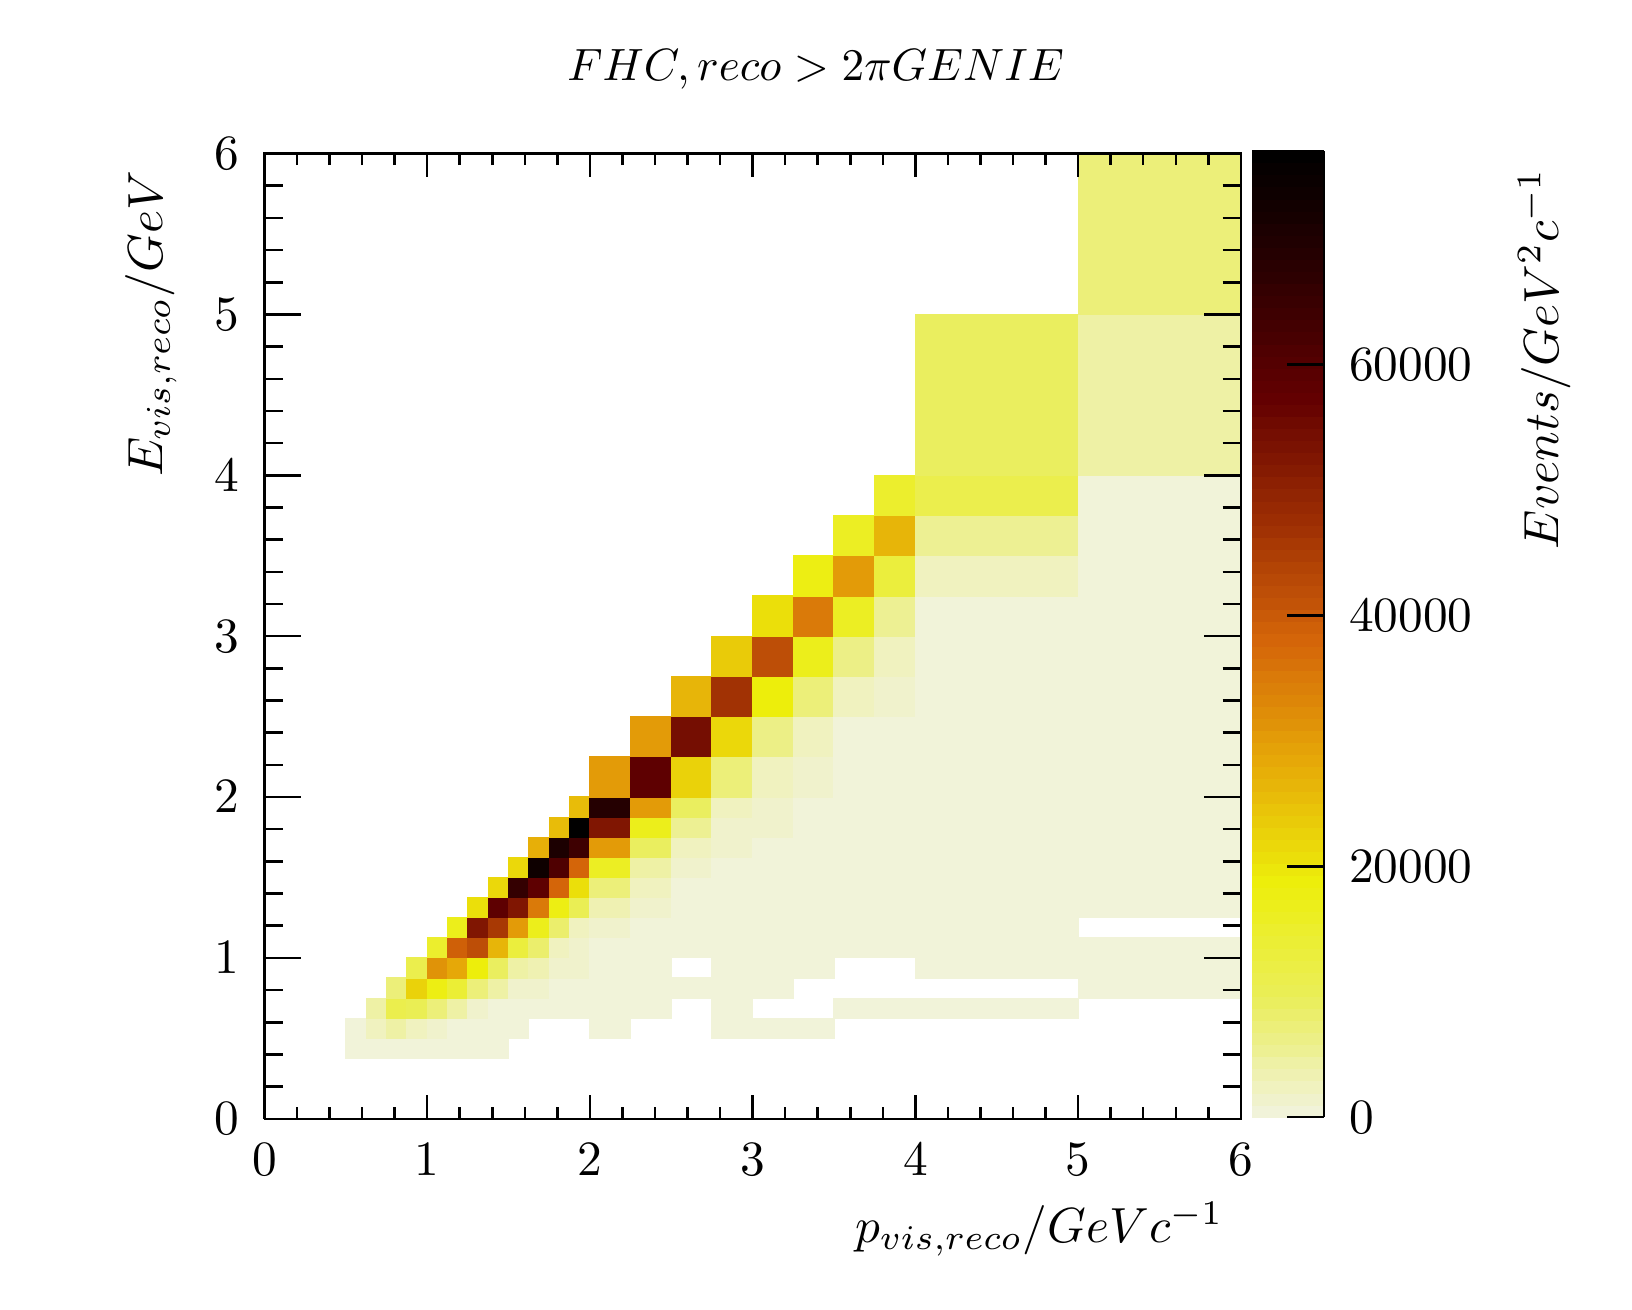
\begin{tikzpicture}
\pgfdeclareplotmark{cross} {
\pgfpathmoveto{\pgfpoint{-0.3\pgfplotmarksize}{\pgfplotmarksize}}
\pgfpathlineto{\pgfpoint{+0.3\pgfplotmarksize}{\pgfplotmarksize}}
\pgfpathlineto{\pgfpoint{+0.3\pgfplotmarksize}{0.3\pgfplotmarksize}}
\pgfpathlineto{\pgfpoint{+1\pgfplotmarksize}{0.3\pgfplotmarksize}}
\pgfpathlineto{\pgfpoint{+1\pgfplotmarksize}{-0.3\pgfplotmarksize}}
\pgfpathlineto{\pgfpoint{+0.3\pgfplotmarksize}{-0.3\pgfplotmarksize}}
\pgfpathlineto{\pgfpoint{+0.3\pgfplotmarksize}{-1.\pgfplotmarksize}}
\pgfpathlineto{\pgfpoint{-0.3\pgfplotmarksize}{-1.\pgfplotmarksize}}
\pgfpathlineto{\pgfpoint{-0.3\pgfplotmarksize}{-0.3\pgfplotmarksize}}
\pgfpathlineto{\pgfpoint{-1.\pgfplotmarksize}{-0.3\pgfplotmarksize}}
\pgfpathlineto{\pgfpoint{-1.\pgfplotmarksize}{0.3\pgfplotmarksize}}
\pgfpathlineto{\pgfpoint{-0.3\pgfplotmarksize}{0.3\pgfplotmarksize}}
\pgfpathclose
\pgfusepathqstroke
}
\pgfdeclareplotmark{cross*} {
\pgfpathmoveto{\pgfpoint{-0.3\pgfplotmarksize}{\pgfplotmarksize}}
\pgfpathlineto{\pgfpoint{+0.3\pgfplotmarksize}{\pgfplotmarksize}}
\pgfpathlineto{\pgfpoint{+0.3\pgfplotmarksize}{0.3\pgfplotmarksize}}
\pgfpathlineto{\pgfpoint{+1\pgfplotmarksize}{0.3\pgfplotmarksize}}
\pgfpathlineto{\pgfpoint{+1\pgfplotmarksize}{-0.3\pgfplotmarksize}}
\pgfpathlineto{\pgfpoint{+0.3\pgfplotmarksize}{-0.3\pgfplotmarksize}}
\pgfpathlineto{\pgfpoint{+0.3\pgfplotmarksize}{-1.\pgfplotmarksize}}
\pgfpathlineto{\pgfpoint{-0.3\pgfplotmarksize}{-1.\pgfplotmarksize}}
\pgfpathlineto{\pgfpoint{-0.3\pgfplotmarksize}{-0.3\pgfplotmarksize}}
\pgfpathlineto{\pgfpoint{-1.\pgfplotmarksize}{-0.3\pgfplotmarksize}}
\pgfpathlineto{\pgfpoint{-1.\pgfplotmarksize}{0.3\pgfplotmarksize}}
\pgfpathlineto{\pgfpoint{-0.3\pgfplotmarksize}{0.3\pgfplotmarksize}}
\pgfpathclose
\pgfusepathqfillstroke
}
\pgfdeclareplotmark{newstar} {
\pgfpathmoveto{\pgfqpoint{0pt}{\pgfplotmarksize}}
\pgfpathlineto{\pgfqpointpolar{44}{0.5\pgfplotmarksize}}
\pgfpathlineto{\pgfqpointpolar{18}{\pgfplotmarksize}}
\pgfpathlineto{\pgfqpointpolar{-20}{0.5\pgfplotmarksize}}
\pgfpathlineto{\pgfqpointpolar{-54}{\pgfplotmarksize}}
\pgfpathlineto{\pgfqpointpolar{-90}{0.5\pgfplotmarksize}}
\pgfpathlineto{\pgfqpointpolar{234}{\pgfplotmarksize}}
\pgfpathlineto{\pgfqpointpolar{198}{0.5\pgfplotmarksize}}
\pgfpathlineto{\pgfqpointpolar{162}{\pgfplotmarksize}}
\pgfpathlineto{\pgfqpointpolar{134}{0.5\pgfplotmarksize}}
\pgfpathclose
\pgfusepathqstroke
}
\pgfdeclareplotmark{newstar*} {
\pgfpathmoveto{\pgfqpoint{0pt}{\pgfplotmarksize}}
\pgfpathlineto{\pgfqpointpolar{44}{0.5\pgfplotmarksize}}
\pgfpathlineto{\pgfqpointpolar{18}{\pgfplotmarksize}}
\pgfpathlineto{\pgfqpointpolar{-20}{0.5\pgfplotmarksize}}
\pgfpathlineto{\pgfqpointpolar{-54}{\pgfplotmarksize}}
\pgfpathlineto{\pgfqpointpolar{-90}{0.5\pgfplotmarksize}}
\pgfpathlineto{\pgfqpointpolar{234}{\pgfplotmarksize}}
\pgfpathlineto{\pgfqpointpolar{198}{0.5\pgfplotmarksize}}
\pgfpathlineto{\pgfqpointpolar{162}{\pgfplotmarksize}}
\pgfpathlineto{\pgfqpointpolar{134}{0.5\pgfplotmarksize}}
\pgfpathclose
\pgfusepathqfillstroke
}
\definecolor{c}{rgb}{1,1,1};
\draw [color=c, fill=c] (0,0) rectangle (20,15.9197);
\draw [color=c, fill=c] (3,2.06957) rectangle (15.4,14.3278);
\definecolor{c}{rgb}{0,0,0};
\draw [c,line width=0.9] (3,2.06957) -- (3,14.3278) -- (15.4,14.3278) -- (15.4,2.06957) -- (3,2.06957);
\definecolor{c}{rgb}{1,1,1};
\draw [color=c, fill=c] (3,2.06957) rectangle (15.4,14.3278);
\definecolor{c}{rgb}{0,0,0};
\draw [c,line width=0.9] (3,2.06957) -- (3,14.3278) -- (15.4,14.3278) -- (15.4,2.06957) -- (3,2.06957);
\definecolor{c}{rgb}{0.945984,0.951044,0.850727};
\draw [color=c, fill=c] (4.03333,2.8357) rectangle (4.29167,3.09108);
\draw [color=c, fill=c] (4.29167,2.8357) rectangle (4.55,3.09108);
\draw [color=c, fill=c] (4.55,2.8357) rectangle (4.80833,3.09108);
\draw [color=c, fill=c] (4.80833,2.8357) rectangle (5.06667,3.09108);
\draw [color=c, fill=c] (5.06667,2.8357) rectangle (5.325,3.09108);
\draw [color=c, fill=c] (5.325,2.8357) rectangle (5.58333,3.09108);
\draw [color=c, fill=c] (5.58333,2.8357) rectangle (5.84167,3.09108);
\draw [color=c, fill=c] (5.84167,2.8357) rectangle (6.1,3.09108);
\draw [color=c, fill=c] (4.03333,3.09108) rectangle (4.29167,3.34646);
\definecolor{c}{rgb}{0.939911,0.947249,0.748261};
\draw [color=c, fill=c] (4.29167,3.09108) rectangle (4.55,3.34646);
\definecolor{c}{rgb}{0.933839,0.943453,0.645794};
\draw [color=c, fill=c] (4.55,3.09108) rectangle (4.80833,3.34646);
\definecolor{c}{rgb}{0.939911,0.947249,0.748261};
\draw [color=c, fill=c] (4.80833,3.09108) rectangle (5.06667,3.34646);
\definecolor{c}{rgb}{0.942948,0.949146,0.799494};
\draw [color=c, fill=c] (5.06667,3.09108) rectangle (5.325,3.34646);
\definecolor{c}{rgb}{0.945984,0.951044,0.850727};
\draw [color=c, fill=c] (5.325,3.09108) rectangle (5.58333,3.34646);
\draw [color=c, fill=c] (5.58333,3.09108) rectangle (5.84167,3.34646);
\draw [color=c, fill=c] (5.84167,3.09108) rectangle (6.1,3.34646);
\draw [color=c, fill=c] (6.1,3.09108) rectangle (6.35833,3.34646);
\draw [color=c, fill=c] (7.13333,3.09108) rectangle (7.65,3.34646);
\draw [color=c, fill=c] (8.68333,3.09108) rectangle (9.2,3.34646);
\draw [color=c, fill=c] (9.2,3.09108) rectangle (9.71667,3.34646);
\draw [color=c, fill=c] (9.71667,3.09108) rectangle (10.2333,3.34646);
\definecolor{c}{rgb}{0.933839,0.943453,0.645794};
\draw [color=c, fill=c] (4.29167,3.34646) rectangle (4.55,3.60184);
\definecolor{c}{rgb}{0.920221,0.933333,0.30049};
\draw [color=c, fill=c] (4.55,3.34646) rectangle (4.80833,3.60184);
\definecolor{c}{rgb}{0.919118,0.933333,0.331373};
\draw [color=c, fill=c] (4.80833,3.34646) rectangle (5.06667,3.60184);
\definecolor{c}{rgb}{0.923719,0.937128,0.475016};
\draw [color=c, fill=c] (5.06667,3.34646) rectangle (5.325,3.60184);
\definecolor{c}{rgb}{0.933839,0.943453,0.645794};
\draw [color=c, fill=c] (5.325,3.34646) rectangle (5.58333,3.60184);
\definecolor{c}{rgb}{0.942948,0.949146,0.799494};
\draw [color=c, fill=c] (5.58333,3.34646) rectangle (5.84167,3.60184);
\definecolor{c}{rgb}{0.945984,0.951044,0.850727};
\draw [color=c, fill=c] (5.84167,3.34646) rectangle (6.1,3.60184);
\draw [color=c, fill=c] (6.1,3.34646) rectangle (6.35833,3.60184);
\draw [color=c, fill=c] (6.35833,3.34646) rectangle (6.61667,3.60184);
\draw [color=c, fill=c] (6.61667,3.34646) rectangle (6.875,3.60184);
\draw [color=c, fill=c] (6.875,3.34646) rectangle (7.13333,3.60184);
\draw [color=c, fill=c] (7.13333,3.34646) rectangle (7.65,3.60184);
\draw [color=c, fill=c] (7.65,3.34646) rectangle (8.16667,3.60184);
\draw [color=c, fill=c] (8.68333,3.34646) rectangle (9.2,3.60184);
\draw [color=c, fill=c] (10.2333,3.34646) rectangle (10.75,3.60184);
\draw [color=c, fill=c] (10.75,3.34646) rectangle (11.2667,3.60184);
\draw [color=c, fill=c] (11.2667,3.34646) rectangle (13.3333,3.60184);
\definecolor{c}{rgb}{0.923719,0.937128,0.475016};
\draw [color=c, fill=c] (4.55,3.60184) rectangle (4.80833,3.85722);
\definecolor{c}{rgb}{0.91826,0.821814,0.0383578};
\draw [color=c, fill=c] (4.80833,3.60184) rectangle (5.06667,3.85722);
\definecolor{c}{rgb}{0.928309,0.933333,0.0740196};
\draw [color=c, fill=c] (5.06667,3.60184) rectangle (5.325,3.85722);
\definecolor{c}{rgb}{0.923529,0.933333,0.207843};
\draw [color=c, fill=c] (5.325,3.60184) rectangle (5.58333,3.85722);
\definecolor{c}{rgb}{0.923719,0.937128,0.475016};
\draw [color=c, fill=c] (5.58333,3.60184) rectangle (5.84167,3.85722);
\definecolor{c}{rgb}{0.933839,0.943453,0.645794};
\draw [color=c, fill=c] (5.84167,3.60184) rectangle (6.1,3.85722);
\definecolor{c}{rgb}{0.942948,0.949146,0.799494};
\draw [color=c, fill=c] (6.1,3.60184) rectangle (6.35833,3.85722);
\draw [color=c, fill=c] (6.35833,3.60184) rectangle (6.61667,3.85722);
\definecolor{c}{rgb}{0.945984,0.951044,0.850727};
\draw [color=c, fill=c] (6.61667,3.60184) rectangle (6.875,3.85722);
\draw [color=c, fill=c] (6.875,3.60184) rectangle (7.13333,3.85722);
\draw [color=c, fill=c] (7.13333,3.60184) rectangle (7.65,3.85722);
\draw [color=c, fill=c] (7.65,3.60184) rectangle (8.16667,3.85722);
\draw [color=c, fill=c] (8.16667,3.60184) rectangle (8.68333,3.85722);
\draw [color=c, fill=c] (8.68333,3.60184) rectangle (9.2,3.85722);
\draw [color=c, fill=c] (9.2,3.60184) rectangle (9.71667,3.85722);
\draw [color=c, fill=c] (13.3333,3.60184) rectangle (15.4,3.85722);
\definecolor{c}{rgb}{0.920221,0.933333,0.30049};
\draw [color=c, fill=c] (4.80833,3.85722) rectangle (5.06667,4.1126);
\definecolor{c}{rgb}{0.879902,0.576716,0.032598};
\draw [color=c, fill=c] (5.06667,3.85722) rectangle (5.325,4.1126);
\definecolor{c}{rgb}{0.901961,0.658824,0.0313726};
\draw [color=c, fill=c] (5.325,3.85722) rectangle (5.58333,4.1126);
\definecolor{c}{rgb}{0.929412,0.933333,0.0431373};
\draw [color=c, fill=c] (5.58333,3.85722) rectangle (5.84167,4.1126);
\definecolor{c}{rgb}{0.917647,0.933333,0.372549};
\draw [color=c, fill=c] (5.84167,3.85722) rectangle (6.1,4.1126);
\definecolor{c}{rgb}{0.933839,0.943453,0.645794};
\draw [color=c, fill=c] (6.1,3.85722) rectangle (6.35833,4.1126);
\definecolor{c}{rgb}{0.936875,0.945351,0.697027};
\draw [color=c, fill=c] (6.35833,3.85722) rectangle (6.61667,4.1126);
\definecolor{c}{rgb}{0.942948,0.949146,0.799494};
\draw [color=c, fill=c] (6.61667,3.85722) rectangle (6.875,4.1126);
\draw [color=c, fill=c] (6.875,3.85722) rectangle (7.13333,4.1126);
\definecolor{c}{rgb}{0.945984,0.951044,0.850727};
\draw [color=c, fill=c] (7.13333,3.85722) rectangle (7.65,4.1126);
\draw [color=c, fill=c] (7.65,3.85722) rectangle (8.16667,4.1126);
\draw [color=c, fill=c] (8.68333,3.85722) rectangle (9.2,4.1126);
\draw [color=c, fill=c] (9.2,3.85722) rectangle (9.71667,4.1126);
\draw [color=c, fill=c] (9.71667,3.85722) rectangle (10.2333,4.1126);
\draw [color=c, fill=c] (11.2667,3.85722) rectangle (13.3333,4.1126);
\draw [color=c, fill=c] (13.3333,3.85722) rectangle (15.4,4.1126);
\definecolor{c}{rgb}{0.924632,0.933333,0.176961};
\draw [color=c, fill=c] (5.06667,4.1126) rectangle (5.325,4.36798);
\definecolor{c}{rgb}{0.810784,0.37549,0.0330882};
\draw [color=c, fill=c] (5.325,4.1126) rectangle (5.58333,4.36798);
\definecolor{c}{rgb}{0.742157,0.306863,0.0257353};
\draw [color=c, fill=c] (5.58333,4.1126) rectangle (5.84167,4.36798);
\definecolor{c}{rgb}{0.907108,0.710294,0.0335784};
\draw [color=c, fill=c] (5.84167,4.1126) rectangle (6.1,4.36798);
\definecolor{c}{rgb}{0.922426,0.933333,0.238725};
\draw [color=c, fill=c] (6.1,4.1126) rectangle (6.35833,4.36798);
\definecolor{c}{rgb}{0.920683,0.935231,0.423782};
\draw [color=c, fill=c] (6.35833,4.1126) rectangle (6.61667,4.36798);
\definecolor{c}{rgb}{0.939911,0.947249,0.748261};
\draw [color=c, fill=c] (6.61667,4.1126) rectangle (6.875,4.36798);
\definecolor{c}{rgb}{0.942948,0.949146,0.799494};
\draw [color=c, fill=c] (6.875,4.1126) rectangle (7.13333,4.36798);
\definecolor{c}{rgb}{0.945984,0.951044,0.850727};
\draw [color=c, fill=c] (7.13333,4.1126) rectangle (7.65,4.36798);
\draw [color=c, fill=c] (7.65,4.1126) rectangle (8.16667,4.36798);
\draw [color=c, fill=c] (8.16667,4.1126) rectangle (8.68333,4.36798);
\draw [color=c, fill=c] (8.68333,4.1126) rectangle (9.2,4.36798);
\draw [color=c, fill=c] (9.2,4.1126) rectangle (9.71667,4.36798);
\draw [color=c, fill=c] (9.71667,4.1126) rectangle (10.2333,4.36798);
\draw [color=c, fill=c] (10.2333,4.1126) rectangle (10.75,4.36798);
\draw [color=c, fill=c] (10.75,4.1126) rectangle (11.2667,4.36798);
\draw [color=c, fill=c] (11.2667,4.1126) rectangle (13.3333,4.36798);
\draw [color=c, fill=c] (13.3333,4.1126) rectangle (15.4,4.36798);
\definecolor{c}{rgb}{0.927206,0.933333,0.104902};
\draw [color=c, fill=c] (5.325,4.36798) rectangle (5.58333,4.62336);
\definecolor{c}{rgb}{0.5,0.0882353,0.00784314};
\draw [color=c, fill=c] (5.58333,4.36798) rectangle (5.84167,4.62336);
\definecolor{c}{rgb}{0.659804,0.22451,0.0169118};
\draw [color=c, fill=c] (5.84167,4.36798) rectangle (6.1,4.62336);
\definecolor{c}{rgb}{0.888726,0.609559,0.0321078};
\draw [color=c, fill=c] (6.1,4.36798) rectangle (6.35833,4.62336);
\definecolor{c}{rgb}{0.927206,0.933333,0.104902};
\draw [color=c, fill=c] (6.35833,4.36798) rectangle (6.61667,4.62336);
\definecolor{c}{rgb}{0.920683,0.935231,0.423782};
\draw [color=c, fill=c] (6.61667,4.36798) rectangle (6.875,4.62336);
\definecolor{c}{rgb}{0.939911,0.947249,0.748261};
\draw [color=c, fill=c] (6.875,4.36798) rectangle (7.13333,4.62336);
\definecolor{c}{rgb}{0.942948,0.949146,0.799494};
\draw [color=c, fill=c] (7.13333,4.36798) rectangle (7.65,4.62336);
\definecolor{c}{rgb}{0.945984,0.951044,0.850727};
\draw [color=c, fill=c] (7.65,4.36798) rectangle (8.16667,4.62336);
\draw [color=c, fill=c] (8.16667,4.36798) rectangle (8.68333,4.62336);
\draw [color=c, fill=c] (8.68333,4.36798) rectangle (9.2,4.62336);
\draw [color=c, fill=c] (9.2,4.36798) rectangle (9.71667,4.62336);
\draw [color=c, fill=c] (9.71667,4.36798) rectangle (10.2333,4.62336);
\draw [color=c, fill=c] (10.2333,4.36798) rectangle (10.75,4.62336);
\draw [color=c, fill=c] (10.75,4.36798) rectangle (11.2667,4.62336);
\draw [color=c, fill=c] (11.2667,4.36798) rectangle (13.3333,4.62336);
\definecolor{c}{rgb}{0.923407,0.873284,0.0405637};
\draw [color=c, fill=c] (5.58333,4.62336) rectangle (5.84167,4.87873);
\definecolor{c}{rgb}{0.368382,0,0.00392157};
\draw [color=c, fill=c] (5.84167,4.62336) rectangle (6.1,4.87873);
\definecolor{c}{rgb}{0.5,0.0882353,0.00784314};
\draw [color=c, fill=c] (6.1,4.62336) rectangle (6.35833,4.87873);
\definecolor{c}{rgb}{0.853431,0.478186,0.0340686};
\draw [color=c, fill=c] (6.35833,4.62336) rectangle (6.61667,4.87873);
\definecolor{c}{rgb}{0.928309,0.933333,0.0740196};
\draw [color=c, fill=c] (6.61667,4.62336) rectangle (6.875,4.87873);
\definecolor{c}{rgb}{0.919118,0.933333,0.331373};
\draw [color=c, fill=c] (6.875,4.62336) rectangle (7.13333,4.87873);
\definecolor{c}{rgb}{0.936875,0.945351,0.697027};
\draw [color=c, fill=c] (7.13333,4.62336) rectangle (7.65,4.87873);
\definecolor{c}{rgb}{0.942948,0.949146,0.799494};
\draw [color=c, fill=c] (7.65,4.62336) rectangle (8.16667,4.87873);
\definecolor{c}{rgb}{0.945984,0.951044,0.850727};
\draw [color=c, fill=c] (8.16667,4.62336) rectangle (8.68333,4.87873);
\draw [color=c, fill=c] (8.68333,4.62336) rectangle (9.2,4.87873);
\draw [color=c, fill=c] (9.2,4.62336) rectangle (9.71667,4.87873);
\draw [color=c, fill=c] (9.71667,4.62336) rectangle (10.2333,4.87873);
\draw [color=c, fill=c] (10.2333,4.62336) rectangle (10.75,4.87873);
\draw [color=c, fill=c] (10.75,4.62336) rectangle (11.2667,4.87873);
\draw [color=c, fill=c] (11.2667,4.62336) rectangle (13.3333,4.87873);
\draw [color=c, fill=c] (13.3333,4.62336) rectangle (15.4,4.87873);
\definecolor{c}{rgb}{0.920833,0.847549,0.0394608};
\draw [color=c, fill=c] (5.84167,4.87873) rectangle (6.1,5.13411);
\definecolor{c}{rgb}{0.202941,0,0.00392157};
\draw [color=c, fill=c] (6.1,4.87873) rectangle (6.35833,5.13411);
\definecolor{c}{rgb}{0.368382,0,0.00392157};
\draw [color=c, fill=c] (6.35833,4.87873) rectangle (6.61667,5.13411);
\definecolor{c}{rgb}{0.831373,0.396078,0.0352941};
\draw [color=c, fill=c] (6.61667,4.87873) rectangle (6.875,5.13411);
\definecolor{c}{rgb}{0.923407,0.873284,0.0405637};
\draw [color=c, fill=c] (6.875,4.87873) rectangle (7.13333,5.13411);
\definecolor{c}{rgb}{0.923719,0.937128,0.475016};
\draw [color=c, fill=c] (7.13333,4.87873) rectangle (7.65,5.13411);
\definecolor{c}{rgb}{0.939911,0.947249,0.748261};
\draw [color=c, fill=c] (7.65,4.87873) rectangle (8.16667,5.13411);
\definecolor{c}{rgb}{0.945984,0.951044,0.850727};
\draw [color=c, fill=c] (8.16667,4.87873) rectangle (8.68333,5.13411);
\draw [color=c, fill=c] (8.68333,4.87873) rectangle (9.2,5.13411);
\draw [color=c, fill=c] (9.2,4.87873) rectangle (9.71667,5.13411);
\draw [color=c, fill=c] (9.71667,4.87873) rectangle (10.2333,5.13411);
\draw [color=c, fill=c] (10.2333,4.87873) rectangle (10.75,5.13411);
\draw [color=c, fill=c] (10.75,4.87873) rectangle (11.2667,5.13411);
\draw [color=c, fill=c] (11.2667,4.87873) rectangle (13.3333,5.13411);
\draw [color=c, fill=c] (13.3333,4.87873) rectangle (15.4,5.13411);
\definecolor{c}{rgb}{0.920833,0.847549,0.0394608};
\draw [color=c, fill=c] (6.1,5.13411) rectangle (6.35833,5.38949);
\definecolor{c}{rgb}{0.0551471,0,0.00122549};
\draw [color=c, fill=c] (6.35833,5.13411) rectangle (6.61667,5.38949);
\definecolor{c}{rgb}{0.308824,0,0.00392157};
\draw [color=c, fill=c] (6.61667,5.13411) rectangle (6.875,5.38949);
\definecolor{c}{rgb}{0.831373,0.396078,0.0352941};
\draw [color=c, fill=c] (6.875,5.13411) rectangle (7.13333,5.38949);
\definecolor{c}{rgb}{0.926103,0.933333,0.135784};
\draw [color=c, fill=c] (7.13333,5.13411) rectangle (7.65,5.38949);
\definecolor{c}{rgb}{0.933839,0.943453,0.645794};
\draw [color=c, fill=c] (7.65,5.13411) rectangle (8.16667,5.38949);
\definecolor{c}{rgb}{0.942948,0.949146,0.799494};
\draw [color=c, fill=c] (8.16667,5.13411) rectangle (8.68333,5.38949);
\definecolor{c}{rgb}{0.945984,0.951044,0.850727};
\draw [color=c, fill=c] (8.68333,5.13411) rectangle (9.2,5.38949);
\draw [color=c, fill=c] (9.2,5.13411) rectangle (9.71667,5.38949);
\draw [color=c, fill=c] (9.71667,5.13411) rectangle (10.2333,5.38949);
\draw [color=c, fill=c] (10.2333,5.13411) rectangle (10.75,5.38949);
\draw [color=c, fill=c] (10.75,5.13411) rectangle (11.2667,5.38949);
\draw [color=c, fill=c] (11.2667,5.13411) rectangle (13.3333,5.38949);
\draw [color=c, fill=c] (13.3333,5.13411) rectangle (15.4,5.38949);
\definecolor{c}{rgb}{0.904534,0.684559,0.0324755};
\draw [color=c, fill=c] (6.35833,5.38949) rectangle (6.61667,5.64487);
\definecolor{c}{rgb}{0.110294,0,0.00245098};
\draw [color=c, fill=c] (6.61667,5.38949) rectangle (6.875,5.64487);
\definecolor{c}{rgb}{0.242647,0,0.00392157};
\draw [color=c, fill=c] (6.875,5.38949) rectangle (7.13333,5.64487);
\definecolor{c}{rgb}{0.888726,0.609559,0.0321078};
\draw [color=c, fill=c] (7.13333,5.38949) rectangle (7.65,5.64487);
\definecolor{c}{rgb}{0.917647,0.933333,0.372549};
\draw [color=c, fill=c] (7.65,5.38949) rectangle (8.16667,5.64487);
\definecolor{c}{rgb}{0.939911,0.947249,0.748261};
\draw [color=c, fill=c] (8.16667,5.38949) rectangle (8.68333,5.64487);
\definecolor{c}{rgb}{0.942948,0.949146,0.799494};
\draw [color=c, fill=c] (8.68333,5.38949) rectangle (9.2,5.64487);
\definecolor{c}{rgb}{0.945984,0.951044,0.850727};
\draw [color=c, fill=c] (9.2,5.38949) rectangle (9.71667,5.64487);
\draw [color=c, fill=c] (9.71667,5.38949) rectangle (10.2333,5.64487);
\draw [color=c, fill=c] (10.2333,5.38949) rectangle (10.75,5.64487);
\draw [color=c, fill=c] (10.75,5.38949) rectangle (11.2667,5.64487);
\draw [color=c, fill=c] (11.2667,5.38949) rectangle (13.3333,5.64487);
\draw [color=c, fill=c] (13.3333,5.38949) rectangle (15.4,5.64487);
\definecolor{c}{rgb}{0.909681,0.736029,0.0346814};
\draw [color=c, fill=c] (6.61667,5.64487) rectangle (6.875,5.90025);
\definecolor{c}{rgb}{0.00551471,0,0.000122549};
\draw [color=c, fill=c] (6.875,5.64487) rectangle (7.13333,5.90025);
\definecolor{c}{rgb}{0.5,0.0882353,0.00784314};
\draw [color=c, fill=c] (7.13333,5.64487) rectangle (7.65,5.90025);
\definecolor{c}{rgb}{0.927206,0.933333,0.104902};
\draw [color=c, fill=c] (7.65,5.64487) rectangle (8.16667,5.90025);
\definecolor{c}{rgb}{0.929791,0.940923,0.577483};
\draw [color=c, fill=c] (8.16667,5.64487) rectangle (8.68333,5.90025);
\definecolor{c}{rgb}{0.942948,0.949146,0.799494};
\draw [color=c, fill=c] (8.68333,5.64487) rectangle (9.2,5.90025);
\draw [color=c, fill=c] (9.2,5.64487) rectangle (9.71667,5.90025);
\definecolor{c}{rgb}{0.945984,0.951044,0.850727};
\draw [color=c, fill=c] (9.71667,5.64487) rectangle (10.2333,5.90025);
\draw [color=c, fill=c] (10.2333,5.64487) rectangle (10.75,5.90025);
\draw [color=c, fill=c] (10.75,5.64487) rectangle (11.2667,5.90025);
\draw [color=c, fill=c] (11.2667,5.64487) rectangle (13.3333,5.90025);
\draw [color=c, fill=c] (13.3333,5.64487) rectangle (15.4,5.90025);
\definecolor{c}{rgb}{0.909681,0.736029,0.0346814};
\draw [color=c, fill=c] (6.875,5.90025) rectangle (7.13333,6.15563);
\definecolor{c}{rgb}{0.143382,0,0.00318627};
\draw [color=c, fill=c] (7.13333,5.90025) rectangle (7.65,6.15563);
\definecolor{c}{rgb}{0.888726,0.609559,0.0321078};
\draw [color=c, fill=c] (7.65,5.90025) rectangle (8.16667,6.15563);
\definecolor{c}{rgb}{0.917647,0.933333,0.372549};
\draw [color=c, fill=c] (8.16667,5.90025) rectangle (8.68333,6.15563);
\definecolor{c}{rgb}{0.939911,0.947249,0.748261};
\draw [color=c, fill=c] (8.68333,5.90025) rectangle (9.2,6.15563);
\definecolor{c}{rgb}{0.942948,0.949146,0.799494};
\draw [color=c, fill=c] (9.2,5.90025) rectangle (9.71667,6.15563);
\definecolor{c}{rgb}{0.945984,0.951044,0.850727};
\draw [color=c, fill=c] (9.71667,5.90025) rectangle (10.2333,6.15563);
\draw [color=c, fill=c] (10.2333,5.90025) rectangle (10.75,6.15563);
\draw [color=c, fill=c] (10.75,5.90025) rectangle (11.2667,6.15563);
\draw [color=c, fill=c] (11.2667,5.90025) rectangle (13.3333,6.15563);
\draw [color=c, fill=c] (13.3333,5.90025) rectangle (15.4,6.15563);
\definecolor{c}{rgb}{0.888726,0.609559,0.0321078};
\draw [color=c, fill=c] (7.13333,6.15563) rectangle (7.65,6.66639);
\definecolor{c}{rgb}{0.368382,0,0.00392157};
\draw [color=c, fill=c] (7.65,6.15563) rectangle (8.16667,6.66639);
\definecolor{c}{rgb}{0.91826,0.821814,0.0383578};
\draw [color=c, fill=c] (8.16667,6.15563) rectangle (8.68333,6.66639);
\definecolor{c}{rgb}{0.923719,0.937128,0.475016};
\draw [color=c, fill=c] (8.68333,6.15563) rectangle (9.2,6.66639);
\definecolor{c}{rgb}{0.939911,0.947249,0.748261};
\draw [color=c, fill=c] (9.2,6.15563) rectangle (9.71667,6.66639);
\definecolor{c}{rgb}{0.942948,0.949146,0.799494};
\draw [color=c, fill=c] (9.71667,6.15563) rectangle (10.2333,6.66639);
\definecolor{c}{rgb}{0.945984,0.951044,0.850727};
\draw [color=c, fill=c] (10.2333,6.15563) rectangle (10.75,6.66639);
\draw [color=c, fill=c] (10.75,6.15563) rectangle (11.2667,6.66639);
\draw [color=c, fill=c] (11.2667,6.15563) rectangle (13.3333,6.66639);
\draw [color=c, fill=c] (13.3333,6.15563) rectangle (15.4,6.66639);
\definecolor{c}{rgb}{0.888726,0.609559,0.0321078};
\draw [color=c, fill=c] (7.65,6.66639) rectangle (8.16667,7.17715);
\definecolor{c}{rgb}{0.458088,0.0551471,0.00637255};
\draw [color=c, fill=c] (8.16667,6.66639) rectangle (8.68333,7.17715);
\definecolor{c}{rgb}{0.920833,0.847549,0.0394608};
\draw [color=c, fill=c] (8.68333,6.66639) rectangle (9.2,7.17715);
\definecolor{c}{rgb}{0.926755,0.939026,0.526249};
\draw [color=c, fill=c] (9.2,6.66639) rectangle (9.71667,7.17715);
\definecolor{c}{rgb}{0.939911,0.947249,0.748261};
\draw [color=c, fill=c] (9.71667,6.66639) rectangle (10.2333,7.17715);
\definecolor{c}{rgb}{0.945984,0.951044,0.850727};
\draw [color=c, fill=c] (10.2333,6.66639) rectangle (10.75,7.17715);
\draw [color=c, fill=c] (10.75,6.66639) rectangle (11.2667,7.17715);
\draw [color=c, fill=c] (11.2667,6.66639) rectangle (13.3333,7.17715);
\draw [color=c, fill=c] (13.3333,6.66639) rectangle (15.4,7.17715);
\definecolor{c}{rgb}{0.907108,0.710294,0.0335784};
\draw [color=c, fill=c] (8.16667,7.17715) rectangle (8.68333,7.6879);
\definecolor{c}{rgb}{0.632353,0.197059,0.0139706};
\draw [color=c, fill=c] (8.68333,7.17715) rectangle (9.2,7.6879);
\definecolor{c}{rgb}{0.929412,0.933333,0.0431373};
\draw [color=c, fill=c] (9.2,7.17715) rectangle (9.71667,7.6879);
\definecolor{c}{rgb}{0.923719,0.937128,0.475016};
\draw [color=c, fill=c] (9.71667,7.17715) rectangle (10.2333,7.6879);
\definecolor{c}{rgb}{0.939911,0.947249,0.748261};
\draw [color=c, fill=c] (10.2333,7.17715) rectangle (10.75,7.6879);
\definecolor{c}{rgb}{0.942948,0.949146,0.799494};
\draw [color=c, fill=c] (10.75,7.17715) rectangle (11.2667,7.6879);
\definecolor{c}{rgb}{0.945984,0.951044,0.850727};
\draw [color=c, fill=c] (11.2667,7.17715) rectangle (13.3333,7.6879);
\draw [color=c, fill=c] (13.3333,7.17715) rectangle (15.4,7.6879);
\definecolor{c}{rgb}{0.915686,0.796078,0.0372549};
\draw [color=c, fill=c] (8.68333,7.6879) rectangle (9.2,8.19866);
\definecolor{c}{rgb}{0.742157,0.306863,0.0257353};
\draw [color=c, fill=c] (9.2,7.6879) rectangle (9.71667,8.19866);
\definecolor{c}{rgb}{0.927206,0.933333,0.104902};
\draw [color=c, fill=c] (9.71667,7.6879) rectangle (10.2333,8.19866);
\definecolor{c}{rgb}{0.926755,0.939026,0.526249};
\draw [color=c, fill=c] (10.2333,7.6879) rectangle (10.75,8.19866);
\definecolor{c}{rgb}{0.939911,0.947249,0.748261};
\draw [color=c, fill=c] (10.75,7.6879) rectangle (11.2667,8.19866);
\definecolor{c}{rgb}{0.945984,0.951044,0.850727};
\draw [color=c, fill=c] (11.2667,7.6879) rectangle (13.3333,8.19866);
\draw [color=c, fill=c] (13.3333,7.6879) rectangle (15.4,8.19866);
\definecolor{c}{rgb}{0.923407,0.873284,0.0405637};
\draw [color=c, fill=c] (9.2,8.19866) rectangle (9.71667,8.70942);
\definecolor{c}{rgb}{0.853431,0.478186,0.0340686};
\draw [color=c, fill=c] (9.71667,8.19866) rectangle (10.2333,8.70942);
\definecolor{c}{rgb}{0.926103,0.933333,0.135784};
\draw [color=c, fill=c] (10.2333,8.19866) rectangle (10.75,8.70942);
\definecolor{c}{rgb}{0.929791,0.940923,0.577483};
\draw [color=c, fill=c] (10.75,8.19866) rectangle (11.2667,8.70942);
\definecolor{c}{rgb}{0.945984,0.951044,0.850727};
\draw [color=c, fill=c] (11.2667,8.19866) rectangle (13.3333,8.70942);
\draw [color=c, fill=c] (13.3333,8.19866) rectangle (15.4,8.70942);
\definecolor{c}{rgb}{0.928309,0.933333,0.0740196};
\draw [color=c, fill=c] (9.71667,8.70942) rectangle (10.2333,9.22018);
\definecolor{c}{rgb}{0.888726,0.609559,0.0321078};
\draw [color=c, fill=c] (10.2333,8.70942) rectangle (10.75,9.22018);
\definecolor{c}{rgb}{0.922426,0.933333,0.238725};
\draw [color=c, fill=c] (10.75,8.70942) rectangle (11.2667,9.22018);
\definecolor{c}{rgb}{0.939911,0.947249,0.748261};
\draw [color=c, fill=c] (11.2667,8.70942) rectangle (13.3333,9.22018);
\definecolor{c}{rgb}{0.945984,0.951044,0.850727};
\draw [color=c, fill=c] (13.3333,8.70942) rectangle (15.4,9.22018);
\definecolor{c}{rgb}{0.926103,0.933333,0.135784};
\draw [color=c, fill=c] (10.2333,9.22018) rectangle (10.75,9.73094);
\definecolor{c}{rgb}{0.907108,0.710294,0.0335784};
\draw [color=c, fill=c] (10.75,9.22018) rectangle (11.2667,9.73094);
\definecolor{c}{rgb}{0.929791,0.940923,0.577483};
\draw [color=c, fill=c] (11.2667,9.22018) rectangle (13.3333,9.73094);
\definecolor{c}{rgb}{0.945984,0.951044,0.850727};
\draw [color=c, fill=c] (13.3333,9.22018) rectangle (15.4,9.73094);
\definecolor{c}{rgb}{0.924632,0.933333,0.176961};
\draw [color=c, fill=c] (10.75,9.73094) rectangle (11.2667,10.2417);
\definecolor{c}{rgb}{0.920221,0.933333,0.30049};
\draw [color=c, fill=c] (11.2667,9.73094) rectangle (13.3333,10.2417);
\definecolor{c}{rgb}{0.945984,0.951044,0.850727};
\draw [color=c, fill=c] (13.3333,9.73094) rectangle (15.4,10.2417);
\definecolor{c}{rgb}{0.917647,0.933333,0.372549};
\draw [color=c, fill=c] (11.2667,10.2417) rectangle (13.3333,12.2847);
\definecolor{c}{rgb}{0.933839,0.943453,0.645794};
\draw [color=c, fill=c] (13.3333,10.2417) rectangle (15.4,12.2847);
\definecolor{c}{rgb}{0.923719,0.937128,0.475016};
\draw [color=c, fill=c] (13.3333,12.2847) rectangle (15.4,14.3278);
\definecolor{c}{rgb}{0,0,0};
\draw [c,line width=0.9] (3,2.06957) -- (15.4,2.06957);
\draw [c,line width=0.9] (3,2.36567) -- (3,2.06957);
\draw [c,line width=0.9] (3.41333,2.21762) -- (3.41333,2.06957);
\draw [c,line width=0.9] (3.82667,2.21762) -- (3.82667,2.06957);
\draw [c,line width=0.9] (4.24,2.21762) -- (4.24,2.06957);
\draw [c,line width=0.9] (4.65333,2.21762) -- (4.65333,2.06957);
\draw [c,line width=0.9] (5.06667,2.36567) -- (5.06667,2.06957);
\draw [c,line width=0.9] (5.48,2.21762) -- (5.48,2.06957);
\draw [c,line width=0.9] (5.89333,2.21762) -- (5.89333,2.06957);
\draw [c,line width=0.9] (6.30667,2.21762) -- (6.30667,2.06957);
\draw [c,line width=0.9] (6.72,2.21762) -- (6.72,2.06957);
\draw [c,line width=0.9] (7.13333,2.36567) -- (7.13333,2.06957);
\draw [c,line width=0.9] (7.54667,2.21762) -- (7.54667,2.06957);
\draw [c,line width=0.9] (7.96,2.21762) -- (7.96,2.06957);
\draw [c,line width=0.9] (8.37333,2.21762) -- (8.37333,2.06957);
\draw [c,line width=0.9] (8.78667,2.21762) -- (8.78667,2.06957);
\draw [c,line width=0.9] (9.2,2.36567) -- (9.2,2.06957);
\draw [c,line width=0.9] (9.61333,2.21762) -- (9.61333,2.06957);
\draw [c,line width=0.9] (10.0267,2.21762) -- (10.0267,2.06957);
\draw [c,line width=0.9] (10.44,2.21762) -- (10.44,2.06957);
\draw [c,line width=0.9] (10.8533,2.21762) -- (10.8533,2.06957);
\draw [c,line width=0.9] (11.2667,2.36567) -- (11.2667,2.06957);
\draw [c,line width=0.9] (11.68,2.21762) -- (11.68,2.06957);
\draw [c,line width=0.9] (12.0933,2.21762) -- (12.0933,2.06957);
\draw [c,line width=0.9] (12.5067,2.21762) -- (12.5067,2.06957);
\draw [c,line width=0.9] (12.92,2.21762) -- (12.92,2.06957);
\draw [c,line width=0.9] (13.3333,2.36567) -- (13.3333,2.06957);
\draw [c,line width=0.9] (13.7467,2.21762) -- (13.7467,2.06957);
\draw [c,line width=0.9] (14.16,2.21762) -- (14.16,2.06957);
\draw [c,line width=0.9] (14.5733,2.21762) -- (14.5733,2.06957);
\draw [c,line width=0.9] (14.9867,2.21762) -- (14.9867,2.06957);
\draw [c,line width=0.9] (15.4,2.36567) -- (15.4,2.06957);
\draw [anchor=base] (3,1.35318) node[scale=1.78272, color=c, rotate=0]{0};
\draw [anchor=base] (5.06667,1.35318) node[scale=1.78272, color=c, rotate=0]{1};
\draw [anchor=base] (7.13333,1.35318) node[scale=1.78272, color=c, rotate=0]{2};
\draw [anchor=base] (9.2,1.35318) node[scale=1.78272, color=c, rotate=0]{3};
\draw [anchor=base] (11.2667,1.35318) node[scale=1.78272, color=c, rotate=0]{4};
\draw [anchor=base] (13.3333,1.35318) node[scale=1.78272, color=c, rotate=0]{5};
\draw [anchor=base] (15.4,1.35318) node[scale=1.78272, color=c, rotate=0]{6};
\draw [anchor= east] (15.4,0.668629) node[scale=1.78272, color=c, rotate=0]{$ p_{vis, reco} / GeV c^{-1}$};
\draw [c,line width=0.9] (3,14.3278) -- (15.4,14.3278);
\draw [c,line width=0.9] (3,14.0317) -- (3,14.3278);
\draw [c,line width=0.9] (3.41333,14.1797) -- (3.41333,14.3278);
\draw [c,line width=0.9] (3.82667,14.1797) -- (3.82667,14.3278);
\draw [c,line width=0.9] (4.24,14.1797) -- (4.24,14.3278);
\draw [c,line width=0.9] (4.65333,14.1797) -- (4.65333,14.3278);
\draw [c,line width=0.9] (5.06667,14.0317) -- (5.06667,14.3278);
\draw [c,line width=0.9] (5.48,14.1797) -- (5.48,14.3278);
\draw [c,line width=0.9] (5.89333,14.1797) -- (5.89333,14.3278);
\draw [c,line width=0.9] (6.30667,14.1797) -- (6.30667,14.3278);
\draw [c,line width=0.9] (6.72,14.1797) -- (6.72,14.3278);
\draw [c,line width=0.9] (7.13333,14.0317) -- (7.13333,14.3278);
\draw [c,line width=0.9] (7.54667,14.1797) -- (7.54667,14.3278);
\draw [c,line width=0.9] (7.96,14.1797) -- (7.96,14.3278);
\draw [c,line width=0.9] (8.37333,14.1797) -- (8.37333,14.3278);
\draw [c,line width=0.9] (8.78667,14.1797) -- (8.78667,14.3278);
\draw [c,line width=0.9] (9.2,14.0317) -- (9.2,14.3278);
\draw [c,line width=0.9] (9.61333,14.1797) -- (9.61333,14.3278);
\draw [c,line width=0.9] (10.0267,14.1797) -- (10.0267,14.3278);
\draw [c,line width=0.9] (10.44,14.1797) -- (10.44,14.3278);
\draw [c,line width=0.9] (10.8533,14.1797) -- (10.8533,14.3278);
\draw [c,line width=0.9] (11.2667,14.0317) -- (11.2667,14.3278);
\draw [c,line width=0.9] (11.68,14.1797) -- (11.68,14.3278);
\draw [c,line width=0.9] (12.0933,14.1797) -- (12.0933,14.3278);
\draw [c,line width=0.9] (12.5067,14.1797) -- (12.5067,14.3278);
\draw [c,line width=0.9] (12.92,14.1797) -- (12.92,14.3278);
\draw [c,line width=0.9] (13.3333,14.0317) -- (13.3333,14.3278);
\draw [c,line width=0.9] (13.7467,14.1797) -- (13.7467,14.3278);
\draw [c,line width=0.9] (14.16,14.1797) -- (14.16,14.3278);
\draw [c,line width=0.9] (14.5733,14.1797) -- (14.5733,14.3278);
\draw [c,line width=0.9] (14.9867,14.1797) -- (14.9867,14.3278);
\draw [c,line width=0.9] (15.4,14.0317) -- (15.4,14.3278);
\draw [c,line width=0.9] (3,2.06957) -- (3,14.3278);
\draw [c,line width=0.9] (3.462,2.06957) -- (3,2.06957);
\draw [c,line width=0.9] (3.231,2.47817) -- (3,2.47817);
\draw [c,line width=0.9] (3.231,2.88678) -- (3,2.88678);
\draw [c,line width=0.9] (3.231,3.29538) -- (3,3.29538);
\draw [c,line width=0.9] (3.231,3.70399) -- (3,3.70399);
\draw [c,line width=0.9] (3.462,4.1126) -- (3,4.1126);
\draw [c,line width=0.9] (3.231,4.5212) -- (3,4.5212);
\draw [c,line width=0.9] (3.231,4.92981) -- (3,4.92981);
\draw [c,line width=0.9] (3.231,5.33842) -- (3,5.33842);
\draw [c,line width=0.9] (3.231,5.74702) -- (3,5.74702);
\draw [c,line width=0.9] (3.462,6.15563) -- (3,6.15563);
\draw [c,line width=0.9] (3.231,6.56424) -- (3,6.56424);
\draw [c,line width=0.9] (3.231,6.97284) -- (3,6.97284);
\draw [c,line width=0.9] (3.231,7.38145) -- (3,7.38145);
\draw [c,line width=0.9] (3.231,7.79006) -- (3,7.79006);
\draw [c,line width=0.9] (3.462,8.19866) -- (3,8.19866);
\draw [c,line width=0.9] (3.231,8.60727) -- (3,8.60727);
\draw [c,line width=0.9] (3.231,9.01587) -- (3,9.01587);
\draw [c,line width=0.9] (3.231,9.42448) -- (3,9.42448);
\draw [c,line width=0.9] (3.231,9.83309) -- (3,9.83309);
\draw [c,line width=0.9] (3.462,10.2417) -- (3,10.2417);
\draw [c,line width=0.9] (3.231,10.6503) -- (3,10.6503);
\draw [c,line width=0.9] (3.231,11.0589) -- (3,11.0589);
\draw [c,line width=0.9] (3.231,11.4675) -- (3,11.4675);
\draw [c,line width=0.9] (3.231,11.8761) -- (3,11.8761);
\draw [c,line width=0.9] (3.462,12.2847) -- (3,12.2847);
\draw [c,line width=0.9] (3.231,12.6933) -- (3,12.6933);
\draw [c,line width=0.9] (3.231,13.1019) -- (3,13.1019);
\draw [c,line width=0.9] (3.231,13.5105) -- (3,13.5105);
\draw [c,line width=0.9] (3.231,13.9192) -- (3,13.9192);
\draw [c,line width=0.9] (3.462,14.3278) -- (3,14.3278);
\draw [anchor= east] (2.9,2.06957) node[scale=1.78272, color=c, rotate=0]{0};
\draw [anchor= east] (2.9,4.1126) node[scale=1.78272, color=c, rotate=0]{1};
\draw [anchor= east] (2.9,6.15563) node[scale=1.78272, color=c, rotate=0]{2};
\draw [anchor= east] (2.9,8.19866) node[scale=1.78272, color=c, rotate=0]{3};
\draw [anchor= east] (2.9,10.2417) node[scale=1.78272, color=c, rotate=0]{4};
\draw [anchor= east] (2.9,12.2847) node[scale=1.78272, color=c, rotate=0]{5};
\draw [anchor= east] (2.9,14.3278) node[scale=1.78272, color=c, rotate=0]{6};
\draw [anchor= east] (1.56,14.3278) node[scale=1.78272, color=c, rotate=90]{$ E_{vis, reco} / GeV$};
\draw [c,line width=0.9] (15.4,2.06957) -- (15.4,14.3278);
\draw [c,line width=0.9] (14.938,2.06957) -- (15.4,2.06957);
\draw [c,line width=0.9] (15.169,2.47817) -- (15.4,2.47817);
\draw [c,line width=0.9] (15.169,2.88678) -- (15.4,2.88678);
\draw [c,line width=0.9] (15.169,3.29538) -- (15.4,3.29538);
\draw [c,line width=0.9] (15.169,3.70399) -- (15.4,3.70399);
\draw [c,line width=0.9] (14.938,4.1126) -- (15.4,4.1126);
\draw [c,line width=0.9] (15.169,4.5212) -- (15.4,4.5212);
\draw [c,line width=0.9] (15.169,4.92981) -- (15.4,4.92981);
\draw [c,line width=0.9] (15.169,5.33842) -- (15.4,5.33842);
\draw [c,line width=0.9] (15.169,5.74702) -- (15.4,5.74702);
\draw [c,line width=0.9] (14.938,6.15563) -- (15.4,6.15563);
\draw [c,line width=0.9] (15.169,6.56424) -- (15.4,6.56424);
\draw [c,line width=0.9] (15.169,6.97284) -- (15.4,6.97284);
\draw [c,line width=0.9] (15.169,7.38145) -- (15.4,7.38145);
\draw [c,line width=0.9] (15.169,7.79006) -- (15.4,7.79006);
\draw [c,line width=0.9] (14.938,8.19866) -- (15.4,8.19866);
\draw [c,line width=0.9] (15.169,8.60727) -- (15.4,8.60727);
\draw [c,line width=0.9] (15.169,9.01587) -- (15.4,9.01587);
\draw [c,line width=0.9] (15.169,9.42448) -- (15.4,9.42448);
\draw [c,line width=0.9] (15.169,9.83309) -- (15.4,9.83309);
\draw [c,line width=0.9] (14.938,10.2417) -- (15.4,10.2417);
\draw [c,line width=0.9] (15.169,10.6503) -- (15.4,10.6503);
\draw [c,line width=0.9] (15.169,11.0589) -- (15.4,11.0589);
\draw [c,line width=0.9] (15.169,11.4675) -- (15.4,11.4675);
\draw [c,line width=0.9] (15.169,11.8761) -- (15.4,11.8761);
\draw [c,line width=0.9] (14.938,12.2847) -- (15.4,12.2847);
\draw [c,line width=0.9] (15.169,12.6933) -- (15.4,12.6933);
\draw [c,line width=0.9] (15.169,13.1019) -- (15.4,13.1019);
\draw [c,line width=0.9] (15.169,13.5105) -- (15.4,13.5105);
\draw [c,line width=0.9] (15.169,13.9192) -- (15.4,13.9192);
\draw [c,line width=0.9] (14.938,14.3278) -- (15.4,14.3278);
\definecolor{c}{rgb}{0.945984,0.951044,0.850727};
\draw [color=c, fill=c] (15.5518,2.0903) rectangle (16.4548,2.24373);
\definecolor{c}{rgb}{0.942948,0.949146,0.799494};
\draw [color=c, fill=c] (15.5518,2.24373) rectangle (16.4548,2.39716);
\definecolor{c}{rgb}{0.939911,0.947249,0.748261};
\draw [color=c, fill=c] (15.5518,2.39716) rectangle (16.4548,2.55059);
\definecolor{c}{rgb}{0.936875,0.945351,0.697027};
\draw [color=c, fill=c] (15.5518,2.55059) rectangle (16.4548,2.70401);
\definecolor{c}{rgb}{0.933839,0.943453,0.645794};
\draw [color=c, fill=c] (15.5518,2.70401) rectangle (16.4548,2.85744);
\definecolor{c}{rgb}{0.929791,0.940923,0.577483};
\draw [color=c, fill=c] (15.5518,2.85744) rectangle (16.4548,3.01087);
\definecolor{c}{rgb}{0.926755,0.939026,0.526249};
\draw [color=c, fill=c] (15.5518,3.01087) rectangle (16.4548,3.1643);
\definecolor{c}{rgb}{0.923719,0.937128,0.475016};
\draw [color=c, fill=c] (15.5518,3.1643) rectangle (16.4548,3.31773);
\definecolor{c}{rgb}{0.920683,0.935231,0.423782};
\draw [color=c, fill=c] (15.5518,3.31773) rectangle (16.4548,3.47115);
\definecolor{c}{rgb}{0.917647,0.933333,0.372549};
\draw [color=c, fill=c] (15.5518,3.47115) rectangle (16.4548,3.62458);
\definecolor{c}{rgb}{0.919118,0.933333,0.331373};
\draw [color=c, fill=c] (15.5518,3.62458) rectangle (16.4548,3.77801);
\definecolor{c}{rgb}{0.920221,0.933333,0.30049};
\draw [color=c, fill=c] (15.5518,3.77801) rectangle (16.4548,3.93144);
\definecolor{c}{rgb}{0.921324,0.933333,0.269608};
\draw [color=c, fill=c] (15.5518,3.93144) rectangle (16.4548,4.08487);
\definecolor{c}{rgb}{0.922426,0.933333,0.238725};
\draw [color=c, fill=c] (15.5518,4.08487) rectangle (16.4548,4.23829);
\definecolor{c}{rgb}{0.923529,0.933333,0.207843};
\draw [color=c, fill=c] (15.5518,4.23829) rectangle (16.4548,4.39172);
\definecolor{c}{rgb}{0.924632,0.933333,0.176961};
\draw [color=c, fill=c] (15.5518,4.39172) rectangle (16.4548,4.54515);
\definecolor{c}{rgb}{0.926103,0.933333,0.135784};
\draw [color=c, fill=c] (15.5518,4.54515) rectangle (16.4548,4.69858);
\definecolor{c}{rgb}{0.927206,0.933333,0.104902};
\draw [color=c, fill=c] (15.5518,4.69858) rectangle (16.4548,4.85201);
\definecolor{c}{rgb}{0.928309,0.933333,0.0740196};
\draw [color=c, fill=c] (15.5518,4.85201) rectangle (16.4548,5.00543);
\definecolor{c}{rgb}{0.929412,0.933333,0.0431373};
\draw [color=c, fill=c] (15.5518,5.00543) rectangle (16.4548,5.15886);
\definecolor{c}{rgb}{0.926838,0.907598,0.0420343};
\draw [color=c, fill=c] (15.5518,5.15886) rectangle (16.4548,5.31229);
\definecolor{c}{rgb}{0.923407,0.873284,0.0405637};
\draw [color=c, fill=c] (15.5518,5.31229) rectangle (16.4548,5.46572);
\definecolor{c}{rgb}{0.920833,0.847549,0.0394608};
\draw [color=c, fill=c] (15.5518,5.46572) rectangle (16.4548,5.61915);
\definecolor{c}{rgb}{0.91826,0.821814,0.0383578};
\draw [color=c, fill=c] (15.5518,5.61915) rectangle (16.4548,5.77257);
\definecolor{c}{rgb}{0.915686,0.796078,0.0372549};
\draw [color=c, fill=c] (15.5518,5.77257) rectangle (16.4548,5.926);
\definecolor{c}{rgb}{0.913113,0.770343,0.036152};
\draw [color=c, fill=c] (15.5518,5.926) rectangle (16.4548,6.07943);
\definecolor{c}{rgb}{0.909681,0.736029,0.0346814};
\draw [color=c, fill=c] (15.5518,6.07943) rectangle (16.4548,6.23286);
\definecolor{c}{rgb}{0.907108,0.710294,0.0335784};
\draw [color=c, fill=c] (15.5518,6.23286) rectangle (16.4548,6.38629);
\definecolor{c}{rgb}{0.904534,0.684559,0.0324755};
\draw [color=c, fill=c] (15.5518,6.38629) rectangle (16.4548,6.53972);
\definecolor{c}{rgb}{0.901961,0.658824,0.0313726};
\draw [color=c, fill=c] (15.5518,6.53972) rectangle (16.4548,6.69314);
\definecolor{c}{rgb}{0.895343,0.634191,0.0317402};
\draw [color=c, fill=c] (15.5518,6.69314) rectangle (16.4548,6.84657);
\definecolor{c}{rgb}{0.888726,0.609559,0.0321078};
\draw [color=c, fill=c] (15.5518,6.84657) rectangle (16.4548,7);
\definecolor{c}{rgb}{0.879902,0.576716,0.032598};
\draw [color=c, fill=c] (15.5518,7) rectangle (16.4548,7.15343);
\definecolor{c}{rgb}{0.873284,0.552083,0.0329657};
\draw [color=c, fill=c] (15.5518,7.15343) rectangle (16.4548,7.30686);
\definecolor{c}{rgb}{0.866667,0.527451,0.0333333};
\draw [color=c, fill=c] (15.5518,7.30686) rectangle (16.4548,7.46028);
\definecolor{c}{rgb}{0.860049,0.502819,0.033701};
\draw [color=c, fill=c] (15.5518,7.46028) rectangle (16.4548,7.61371);
\definecolor{c}{rgb}{0.853431,0.478186,0.0340686};
\draw [color=c, fill=c] (15.5518,7.61371) rectangle (16.4548,7.76714);
\definecolor{c}{rgb}{0.844608,0.445343,0.0345588};
\draw [color=c, fill=c] (15.5518,7.76714) rectangle (16.4548,7.92057);
\definecolor{c}{rgb}{0.83799,0.420711,0.0349265};
\draw [color=c, fill=c] (15.5518,7.92057) rectangle (16.4548,8.074);
\definecolor{c}{rgb}{0.831373,0.396078,0.0352941};
\draw [color=c, fill=c] (15.5518,8.074) rectangle (16.4548,8.22742);
\definecolor{c}{rgb}{0.810784,0.37549,0.0330882};
\draw [color=c, fill=c] (15.5518,8.22742) rectangle (16.4548,8.38085);
\definecolor{c}{rgb}{0.790196,0.354902,0.0308824};
\draw [color=c, fill=c] (15.5518,8.38085) rectangle (16.4548,8.53428);
\definecolor{c}{rgb}{0.762745,0.327451,0.0279412};
\draw [color=c, fill=c] (15.5518,8.53428) rectangle (16.4548,8.68771);
\definecolor{c}{rgb}{0.742157,0.306863,0.0257353};
\draw [color=c, fill=c] (15.5518,8.68771) rectangle (16.4548,8.84114);
\definecolor{c}{rgb}{0.721569,0.286275,0.0235294};
\draw [color=c, fill=c] (15.5518,8.84114) rectangle (16.4548,8.99457);
\definecolor{c}{rgb}{0.70098,0.265686,0.0213235};
\draw [color=c, fill=c] (15.5518,8.99457) rectangle (16.4548,9.14799);
\definecolor{c}{rgb}{0.680392,0.245098,0.0191176};
\draw [color=c, fill=c] (15.5518,9.14799) rectangle (16.4548,9.30142);
\definecolor{c}{rgb}{0.659804,0.22451,0.0169118};
\draw [color=c, fill=c] (15.5518,9.30142) rectangle (16.4548,9.45485);
\definecolor{c}{rgb}{0.632353,0.197059,0.0139706};
\draw [color=c, fill=c] (15.5518,9.45485) rectangle (16.4548,9.60828);
\definecolor{c}{rgb}{0.611765,0.176471,0.0117647};
\draw [color=c, fill=c] (15.5518,9.60828) rectangle (16.4548,9.76171);
\definecolor{c}{rgb}{0.590809,0.159926,0.0110294};
\draw [color=c, fill=c] (15.5518,9.76171) rectangle (16.4548,9.91513);
\definecolor{c}{rgb}{0.569853,0.143382,0.0102941};
\draw [color=c, fill=c] (15.5518,9.91513) rectangle (16.4548,10.0686);
\definecolor{c}{rgb}{0.548897,0.126838,0.00955882};
\draw [color=c, fill=c] (15.5518,10.0686) rectangle (16.4548,10.222);
\definecolor{c}{rgb}{0.520956,0.104779,0.00857843};
\draw [color=c, fill=c] (15.5518,10.222) rectangle (16.4548,10.3754);
\definecolor{c}{rgb}{0.5,0.0882353,0.00784314};
\draw [color=c, fill=c] (15.5518,10.3754) rectangle (16.4548,10.5288);
\definecolor{c}{rgb}{0.479044,0.0716912,0.00710784};
\draw [color=c, fill=c] (15.5518,10.5288) rectangle (16.4548,10.6823);
\definecolor{c}{rgb}{0.458088,0.0551471,0.00637255};
\draw [color=c, fill=c] (15.5518,10.6823) rectangle (16.4548,10.8357);
\definecolor{c}{rgb}{0.437132,0.0386029,0.00563726};
\draw [color=c, fill=c] (15.5518,10.8357) rectangle (16.4548,10.9891);
\definecolor{c}{rgb}{0.409191,0.0165441,0.00465686};
\draw [color=c, fill=c] (15.5518,10.9891) rectangle (16.4548,11.1426);
\definecolor{c}{rgb}{0.388235,0,0.00392157};
\draw [color=c, fill=c] (15.5518,11.1426) rectangle (16.4548,11.296);
\definecolor{c}{rgb}{0.368382,0,0.00392157};
\draw [color=c, fill=c] (15.5518,11.296) rectangle (16.4548,11.4494);
\definecolor{c}{rgb}{0.348529,0,0.00392157};
\draw [color=c, fill=c] (15.5518,11.4494) rectangle (16.4548,11.6028);
\definecolor{c}{rgb}{0.328676,0,0.00392157};
\draw [color=c, fill=c] (15.5518,11.6028) rectangle (16.4548,11.7563);
\definecolor{c}{rgb}{0.308824,0,0.00392157};
\draw [color=c, fill=c] (15.5518,11.7563) rectangle (16.4548,11.9097);
\definecolor{c}{rgb}{0.282353,0,0.00392157};
\draw [color=c, fill=c] (15.5518,11.9097) rectangle (16.4548,12.0631);
\definecolor{c}{rgb}{0.2625,0,0.00392157};
\draw [color=c, fill=c] (15.5518,12.0631) rectangle (16.4548,12.2166);
\definecolor{c}{rgb}{0.242647,0,0.00392157};
\draw [color=c, fill=c] (15.5518,12.2166) rectangle (16.4548,12.37);
\definecolor{c}{rgb}{0.222794,0,0.00392157};
\draw [color=c, fill=c] (15.5518,12.37) rectangle (16.4548,12.5234);
\definecolor{c}{rgb}{0.202941,0,0.00392157};
\draw [color=c, fill=c] (15.5518,12.5234) rectangle (16.4548,12.6768);
\definecolor{c}{rgb}{0.176471,0,0.00392157};
\draw [color=c, fill=c] (15.5518,12.6768) rectangle (16.4548,12.8303);
\definecolor{c}{rgb}{0.159926,0,0.00355392};
\draw [color=c, fill=c] (15.5518,12.8303) rectangle (16.4548,12.9837);
\definecolor{c}{rgb}{0.143382,0,0.00318627};
\draw [color=c, fill=c] (15.5518,12.9837) rectangle (16.4548,13.1371);
\definecolor{c}{rgb}{0.126838,0,0.00281863};
\draw [color=c, fill=c] (15.5518,13.1371) rectangle (16.4548,13.2906);
\definecolor{c}{rgb}{0.110294,0,0.00245098};
\draw [color=c, fill=c] (15.5518,13.2906) rectangle (16.4548,13.444);
\definecolor{c}{rgb}{0.0882353,0,0.00196078};
\draw [color=c, fill=c] (15.5518,13.444) rectangle (16.4548,13.5974);
\definecolor{c}{rgb}{0.0716912,0,0.00159314};
\draw [color=c, fill=c] (15.5518,13.5974) rectangle (16.4548,13.7508);
\definecolor{c}{rgb}{0.0551471,0,0.00122549};
\draw [color=c, fill=c] (15.5518,13.7508) rectangle (16.4548,13.9043);
\definecolor{c}{rgb}{0.0386029,0,0.000857843};
\draw [color=c, fill=c] (15.5518,13.9043) rectangle (16.4548,14.0577);
\definecolor{c}{rgb}{0.0220588,0,0.000490196};
\draw [color=c, fill=c] (15.5518,14.0577) rectangle (16.4548,14.2111);
\definecolor{c}{rgb}{0.00551471,0,0.000122549};
\draw [color=c, fill=c] (15.5518,14.2111) rectangle (16.4548,14.3645);
\definecolor{c}{rgb}{0,0,0};
\draw [c,line width=0.9] (16.4548,2.0903) -- (16.4548,14.3645);
\draw [c,line width=0.9] (15.9922,2.0903) -- (16.4548,2.0903);
\draw [c,line width=0.9] (15.9922,5.2757) -- (16.4548,5.2757);
\draw [c,line width=0.9] (15.9922,8.4611) -- (16.4548,8.4611);
\draw [c,line width=0.9] (15.9922,11.6465) -- (16.4548,11.6465);
\draw [c,line width=0.9] (15.9922,11.6465) -- (16.4548,11.6465);
\draw [anchor= west] (16.5548,2.0903) node[scale=1.78272, color=c, rotate=0]{0};
\draw [anchor= west] (16.5548,5.2757) node[scale=1.78272, color=c, rotate=0]{20000};
\draw [anchor= west] (16.5548,8.4611) node[scale=1.78272, color=c, rotate=0]{40000};
\draw [anchor= west] (16.5548,11.6465) node[scale=1.78272, color=c, rotate=0]{60000};
\draw [anchor= east] (19.2549,14.3645) node[scale=1.78272, color=c, rotate=90]{$Events / GeV^{2}c^{-1}$};
\definecolor{c}{rgb}{1,1,1};
\draw [color=c, fill=c] (2,14.9645) rectangle (18,15.8401);
\definecolor{c}{rgb}{0,0,0};
\draw (10,15.4023) node[scale=1.63416, color=c, rotate=0]{$FHC, reco >2\pi GENIE$};
\end{tikzpicture}

		\end{adjustbox}
	\end{subfigure}
\end{figure}
